%\documentclass[a4paper,12pt,twoside]{book}
\documentclass[listof=nochaptergap,12pt,times,authoryear]{report}
\usepackage{mathptmx}%This package supersedes times and mathptm
\usepackage[a4paper,right=2.54cm,left=2.54cm,top=2.54cm,bottom=2.54cm]{geometry}
\usepackage{array}
\usepackage{listings}
\usepackage{pdflscape}
\usepackage{longtable}
\usepackage{enumitem}
\usepackage{newclude}
\usepackage{float}
\usepackage{comment}
\usepackage[export]{adjustbox}
\usepackage{algorithm}
\usepackage{algpseudocode}

\floatname{algorithm}{Algoritmo}

\newcolumntype{C}[1]{>{\centering\arraybackslash}p{#1}}
\newcolumntype{N}{@{}m{0pt}@{}}
\newcommand\fillin[1][3cm]{\makebox[#1]{\dotfill}}

%%Paquete para ocultar indices de tabla de contenidos
%% Numeración continua en figuras y tablas
\setcounter{equation}{0}
\usepackage{chngcntr}
\counterwithout{figure}{chapter}
\counterwithout{table}{chapter}
\counterwithout{equation}{chapter}
\renewcommand{\thefigure}{\arabic{figure}}
\renewcommand{\thetable}{\arabic{table}}
\renewcommand{\theequation}{\arabic{equation}}

% Parche para eliminar espacios por capítulos en lista de figuras y tablas
\usepackage{etoolbox}% http://ctan.org/pkg/etoolbox
\makeatletter
% \patchcmd{<cmd>}{<search>}{<replace>}{<succes>}{<failure>}
\patchcmd{\@chapter}{\addtocontents{lof}{\protect\addvspace{10\p@}}}{}{}{}% LoF
\patchcmd{\@chapter}{\addtocontents{lot}{\protect\addvspace{10\p@}}}{}{}{}% LoT
\makeatother


%%%%paquete para usar citas de diferentes formatos
%%%%%%%%%%%%%%%%%%%%%%%%%%%%%%%%%
%%add al indice
%\usepackage[nottoc,numbib]{tocbibind}
%\usepackage[authoryear,round]{natbib}
\usepackage[utf8]{inputenc}
\usepackage{csquotes}
\usepackage[spanish,es-lcroman]{babel}
\decimalpoint
%% Citas y bibliografía formato APA
\usepackage[backend=biber,style=apa,natbib=true]{biblatex}
%\DeclareLanguageMapping{australian}{australian-apa}
\DeclareLanguageMapping{spanish}{spanish-apa}
\addbibresource{biblio/references.bib}

%% Formato DOI
\DeclareFieldFormat{doi}{%
	doi\addcolon\space
	\ifhyperref
	{\lowercase{\href{https://doi.org/#1}{\nolinkurl{#1}}}}
	{\lowercase{\nolinkurl{#1}}}}

%% Formato de URL en referencias
\DeclareFieldFormat{url}{{Recuperado de}\space\url{#1}}

%% Convertir comando cita por textcite para que tenga formato APA
\let\cite\textcite

%% Para que texto de figuras y tablas tenga formato APA
\usepackage{multirow,booktabs,setspace,caption}
\DeclareCaptionLabelSeparator*{spaced}{\\[2ex]}
\captionsetup[table]{labelfont=normalfont,textfont=it,format=plain,justification=justified,singlelinecheck=false,labelsep=newline,skip=2pt}
\captionsetup[figure]{labelsep=period,labelfont={it,bf},justification=justified,singlelinecheck=false,font=doublespacing}
\captionsetup[subfigure]{justification=centering}

%%%Editar formato y tamaño de capítulos y secciones
\usepackage{titlesec}
\titleformat{\chapter}
{\centering\normalfont\large\bfseries}{Capítulo \thechapter:}{1em}{}
\titlespacing*{\chapter}{0pt}{-4ex}{1ex}

\titleformat{\section}
{\normalfont\large\bfseries}{\thesection}{1em}{}
\titlespacing*{\section}{0pt}{0pt}{0pt}

\titleformat{\subsection}
{\normalfont\large\bfseries}{\thesubsection}{1em}{}
\titlespacing*{\subsection}{0pt}{0pt}{0pt}

%\usepackage{biblatex}
%paquete para hiperlinks entre citas e imagenes
%%%%%%%%%%%%%%%%%%%%%%%%%%%%%%%%%
\usepackage[colorlinks=true,
citecolor=black,
urlcolor=black,
bookmarks=true,
linkcolor=black,
pdftitle={Tesis-nombre-alumno},
pdfauthor={autor nombres}]{hyperref}

\usepackage{amssymb}
\usepackage{graphicx} % for improved inclusion of graphics
%\usepackage{wrapfig} % to include figure with text wrapping around it
\usepackage[margin=10pt,font=small,labelfont=bf]{caption} % for improved layout of figure captions with extra margin, smaller font than text
\usepackage{subcaption}
\usepackage{eucal}
\usepackage[usenames, dvipsnames]{color}
\usepackage[perpage]{footmisc}
%\usepackage[round, sort]{natbib}
\usepackage{ifthen}
\usepackage{multicol} % for pages with multiple text columns, e.g. References
\setlength{\columnsep}{20pt} % space between columns; default 10pt quite narrow
%% Para no mostrar índices de figuras ni tablas en el índice general
\usepackage[nottoc,notlot,notlof]{tocbibind}
%\usepackage{appendix}
\usepackage[titletoc,title]{appendix} 

%%%----Modificar encabezado y pie de pagina
%%%%%%%%%%%%%%%%%%%%%%%%%%%%%%%%%%%%%%%%%%%%%%%%%%%%%%%%%%%%%%%%%%%%%
\usepackage{fancyhdr} % for better header layout
\newcommand{\changefont}{%
	\fontsize{9pt}{1.5pt}\selectfont
}

\pagestyle{fancy}
%%Para borrar fancy por default (incluye numeracion)
\fancyhf{} % sets both header and footer to nothing
%%Para borrar linea de encabezado
\renewcommand{\headrulewidth}{0pt}
%%Encabezados solo con numero de pagina
\fancypagestyle{normal}{%
	\fancyhead{} % clear all header fields
	\fancyhead[R]{\thepage}}
%%Encabezados con titulo de tesis y numero de pagina
\fancypagestyle{special}{%
	\fancyhead[L]{\changefont Propuesta de modelo de clasificación automatizada de deterioros en pavimentos de Lima
	Metropolitana, Perú utilizando Redes Neuronales Convolucionales}
	\fancyhead[R]{\thepage}}


%\fancyhf{} %% delete default configuration of page
%%\setlength\headheight{15pt}

%%%%%%%%%%%%%%%%%%%%%%%%%%%%%5
%%%% Configuracion de los parrafos
%\usepackage{setspace}
%\onehalfspacing
%\linespread{1.25} 
\setlength{\parindent}{0.5in} %%sangria
\setlength{\parskip}{3mm}  %%espacio entre parrafos
\linespread{1.3} %This equals 1.5 linespacing in Word
%%%% nuevo parrafo
%%%%%%%%%%%%%%%%%%%%%%%%%%%%%5
%%%% Centrar valores de una tabla
\usepackage{array}
%%CENTRADO HORIZONTAL
\newcolumntype{P}[1]{>{\centering\arraybackslash}p{#1}}
%%CENTRADO VERTICAL
\newcolumntype{M}[1]{>{\centering\arraybackslash}m{#1}}

%%%%%%%%%%%%%%%%%%%%%%%%%%%%%5
%%%%Paquete para alinear texto
\usepackage{ragged2e}
\usepackage{multirow}
\usepackage{makecell}
\usepackage{rotating}
\usepackage{siunitx} % To align the numbers later on
\usepackage[table,xcdraw]{xcolor}
\usepackage{color, colortbl}
\definecolor{Gray}{gray}{0.9}
\definecolor{orange}{rgb}{1,0.647,0}
\definecolor{turq3}{rgb}{0.54, 0.81, 0.94}
\definecolor{turq}{rgb}{0.63, 0.79, 0.95}
\definecolor{bluejean}{rgb}{0.03, 0.27, 0.49}

%%%%%%%%%%%%%%%%%%%%%%%%%
\usepackage{xparse}
\usepackage{expl3}
%%%%funcion de reemplazar regex
\ExplSyntaxOn
\NewDocumentCommand{\replace}{mmm}
{
	\marian_replace:nnn {#1} {#2} {#3}
}

\tl_new:N \l_marian_input_text_tl
\tl_new:N \l_marian_search_tl
\tl_new:N \l_marian_replace_tl

\cs_new_protected:Npn \marian_replace:nnn #1 #2 #3
{
	\tl_set:Nn \l_marian_input_text_tl { #1 }
	\tl_set:Nn \l_marian_search_tl { #2 }
	\tl_set:Nn \l_marian_replace_tl { #3 }
	\regex_replace_all:nnN { \b\u{l_marian_search_tl}\b } { \u{l_marian_replace_tl} } \l_marian_input_text_tl
	\tl_use:N \l_marian_input_text_tl
}
\ExplSyntaxOff

%%%%%%%%%%%%%%%%%%%%%%%%%%%%%%%%%%%%%%
\usepackage{amsmath}
%\setcounter{equation}{0}
%\numberwithin{equation}{chapter} %%enumerar ecuaciones
%\renewcommand{\theequation}{Ecuación \arabic{equation}}   
\usepackage{mathtools, nccmath, cool}
%%%Configuraciones de biblatex

%%%hel
%%%%\citeauthor
\makeatletter

%%%%%%%%%%%%
\DeclareCiteCommand{\citeauthor}
{\boolfalse{citetracker}%
	\boolfalse{pagetracker}%
	\usebibmacro{prenote}}
{\ifciteindex
	{\indexnames{labelname}}
	{}%
	\printtext[bibhyperref]{\printnames{labelname}}}
{\multicitedelim}
{\usebibmacro{postnote}}


\DeclareCiteCommand{\citetitle}
{\boolfalse{citetracker}%
	\boolfalse{pagetracker}%
	\usebibmacro{prenote}}
{\ifciteindex
	{\indexfield{indextitle}}
	{}%
	\printtext[bibhyperref]{\printfield[citetitle]{labeltitle}}}
{\multicitedelim}
{\usebibmacro{postnote}}

\DeclareCiteCommand{\cite}
{\usebibmacro{prenote}}
{\usebibmacro{citeindex}%
	\printtext[bibhyperref]{\usebibmacro{cite}}}
{\multicitedelim}
{\usebibmacro{postnote}}

\DeclareCiteCommand*{\cite}
{\usebibmacro{prenote}}
{\usebibmacro{citeindex}%
	\printtext[bibhyperref]{\usebibmacro{citeyear}}}
{\multicitedelim}
{\usebibmacro{postnote}}

\DeclareCiteCommand{\parencite}[\mkbibparens]
{\usebibmacro{prenote}}
{\usebibmacro{citeindex}%
	\printtext[bibhyperref]{\usebibmacro{cite}}}
{\multicitedelim}
{\usebibmacro{postnote}}

\DeclareCiteCommand*{\parencite}[\mkbibparens]
{\usebibmacro{prenote}}
{\usebibmacro{citeindex}%
	\printtext[bibhyperref]{\usebibmacro{citeyear}}}
{\multicitedelim}
{\usebibmacro{postnote}}

\DeclareCiteCommand{\footcite}[\mkbibfootnote]
{\usebibmacro{prenote}}
{\usebibmacro{citeindex}%
	\printtext[bibhyperref]{ \usebibmacro{cite}}}
{\multicitedelim}
{\usebibmacro{postnote}}

\DeclareCiteCommand{\footcitetext}[\mkbibfootnotetext]
{\usebibmacro{prenote}}
{\usebibmacro{citeindex}%
	\printtext[bibhyperref]{\usebibmacro{cite}}}
{\multicitedelim}
{\usebibmacro{postnote}}

\DeclareCiteCommand{\textcite}
{\boolfalse{cbx:parens}}
{\usebibmacro{citeindex}%
	\printtext[bibhyperref]{\usebibmacro{textcite}}}
{\ifbool{cbx:parens}
	{\bibcloseparen\global\boolfalse{cbx:parens}}
	{}%
	\multicitedelim}
{\usebibmacro{textcite:postnote}}
\makeatother
\makeatletter
\let\abx@macro@citeOrig\abx@macro@cite
\renewbibmacro{cite}{%
	\bibhyperref{%
		\let\bibhyperref\relax\relax%
		\abx@macro@citeOrig%
	}%
}
\let\abx@macro@textciteOrig\abx@macro@textcite
\renewbibmacro{textcite}{%
	\bibhyperref{%
		\let\bibhyperref\relax\relax%
		\abx@macro@textciteOrig%
	}%
}%

\makeatother

%%%%%%%%%%%%%%%%%%%%%%%%%%%%%%%%%%%%%%%%%%%
% Agregando librerias para que aparezca texto debajo de las ecuaciones.
\usepackage[titles]{tocloft}

%% Para agregar palabra "CAPÍTULO" en 
\newlength\mynewlength
\let\oldcftchappresnum\cftchappresnum
\renewcommand*\cftchappresnum{Capítulo \oldcftchappresnum}
\renewcommand\cftchapaftersnum{:}
\settowidth\mynewlength{\cftchappresnum\cftchapaftersnum\quad}
\addtolength\cftchapnumwidth{\mynewlength}

\usepackage{xpatch}
\usepackage{caption}
\DeclareCaptionType{equcaption}[Ecuación][Índice de Ecuaciones]

\newenvironment{conditions}
{\par\vspace{\abovedisplayskip}\noindent\begin{tabular}{>{$}l<{$} @{${}={}$} l}}
	{\end{tabular}\par\vspace{\belowdisplayskip}}

% Para agregar linea de puntos en la tabla de contenidos
\renewcommand{\cftpartleader}{\cftdotfill{\cftdotsep}} % for parts
\renewcommand{\cftchapleader}{\cftdotfill{\cftdotsep}} % for chapters

% Para eliminar linea de puntos de la tabla de contenidos
%\renewcommand{\cftdot}{}

% Para alinear párrafo en indice de figuras y tablas
\cftsetindents{figure}{0em}{2.5em}
\renewcommand\cftfigpresnum{\figurename~}
\renewcommand{\cftfigaftersnum}{.} % Goes after figure number
\newlength\mylength
\settowidth\mylength{\cftfigpresnum}
\addtolength\cftfignumwidth{\mylength}
\cftsetindents{table}{0em}{2.5em}
\renewcommand\cfttabpresnum{Tabla }
\renewcommand{\cfttabaftersnum}{.} % Goes after figure number
\settowidth\mylength{\cfttabpresnum}
\addtolength\cfttabnumwidth{\mylength}

\DefineBibliographyExtras{spanish}{%
	\savecommand\sptext
	\renewcommand*{\sptext}{\textsuperscript}}

\UndefineBibliographyExtras{spanish}{%
	\restorecommand\sptext}

%%Formato APA (No funciona en biblatex)
\usepackage{apalike}
%\bibliographystyle{apalike}

\begin{document}
% Se añade esto para agregar la lista de ecuaciones en el indice del documento	

\newcommand{\listequationsname}{Índice de Ecuaciones}
\newlistof{myequations}{equ}{\listequationsname}
\newcommand{\myequations}[1]{%
	\addcontentsline{equ}{myequations}{Ecuación \protect\numberline{\theequation}#1}\par}
%\addcontentsline{toc}{section}{Índice de Ecuaciones}

%%Numeros de pagina en romano (minuscula)
%\pagenumbering{roman}
\renewcommand{\thepage}{\roman{page}}

% Beginning of hack...
%\let\oldthispagestyle=\thispagestyle % If we want to see a page number.
%\def\thispagestyle#1{} % If we want to see a page number.
%\let\oldsetcounter=\setcounter
%\def\setcounter#1#2{}
% End of hack...

\begin{titlepage}

	\begin{center}
		%%%cargar imagen
	    
\includegraphics[width=0.20\textwidth]{images_repo/esanlogomin}
		\vspace*{2cm} \\
		UNIVERSIDAD ESAN \vspace*{1ex} \\
		FACULTAD DE INGENIERÍA \vspace*{1ex} \\
		INGENIERÍA DE TECNOLOGÍAS DE INFORMACIÓN Y SISTEMAS
		\vspace*{8ex} \\
		%\textbf
		{Propuesta de modelo de clasificación automatizada de deterioros en pavimentos de Lima Metropolitana, Perú utilizando Redes Neuronales Convolucionales}
		\vspace*{8ex}\\	
		Tesis de investigación para el curso Trabajo de Tesis I 
		\vspace*{8ex} \\	
		Hernan  Marecos  \\
		Asesor: Marks Calderón		
		\vfill
		Lima, \today 
		
	\end{center}
\end{titlepage}
%%Permite mostrar encabezado y numeracion en primera pagina de capitulos - indices
\fancypagestyle{plain}{}
%%cambiar nombres de objetos para el indice y otros
\renewcommand{\listfigurename}{Índice de Figuras}
\renewcommand{\tablename}{Tabla}
\renewcommand{\listtablename}{Índice de Tablas}
\renewcommand{\listalgorithmname}{Índice de Algoritmos}

%%Permite empezar conteo de paginas de forma personalizada
\addtocounter{page}{1}
\pagestyle{normal}
%\thispagestyle{plain}
%\vspace{0.5cm}
\leftline{Esta tesis denominada:}
\begin{center}
	%\vspace*{10cm}
	{PROPUESTA DE MODELO DE CLASIFICACIÓN AUTOMATIZADA DE DETERIOROS EN PAVIMENTOS DE LIMA METROPOLITANA, PERÚ UTILIZANDO REDES NEURONALES CONVOLUCIONALES}
\end{center}

\leftline{ha sido aprobada.}
\vspace{3cm}

%\dotfill
\rightline{\fillin[9cm]}
\rightline{Jurado 1}
\vspace{3cm}

%\dotfill
\rightline{\fillin[9cm]}
\rightline{Jurado 2}
\vspace{3cm}

%\dotfill
\rightline{\fillin[9cm]}
\rightline{Jurado 3}
\vspace{3cm}

\centerline{Universidad ESAN}
\centerline{2024}
%\thispagestyle{plain}
\begin{center}
	\vspace*{10cm}
	{PROPUESTA DE MODELO DE CLASIFICACIÓN AUTOMATIZADA DE DETERIOROS EN PAVIMENTOS DE LIMA METROPOLITANA, PERÚ UTILIZANDO REDES NEURONALES CONVOLUCIONALES}
\end{center}

%\thispagestyle{plain}
\begin{center}
	%\vspace*{1.5cm}
	{\large \bfseries  Dedicatoria}
\end{center}
\vspace{0.5cm}

A mi madre.

Sin ti nada de esto hubiera sido posible te debo todo.
\newline



% outline
\tableofcontents            % print the table of contents

%: ----------------------- contents ------------------------

\setcounter{secnumdepth}{3} % organisational level that receives a numbers
\setcounter{tocdepth}{3}    % print table of contents for level 3

% levels are: 0 - chapter, 1 - section, 2 - subsection, 3 - subsection


%: ----------------------- list of figures/tables ------------------------
\clearpage
\listoffigures
\clearpage
\listoftables  % print list of tables
\clearpage
\phantomsection
%\listofequcaptions % print list of equations
\listofmyequations
\clearpage
\listofalgorithms
\clearpage
%% Numeros de pagina en arabic (si se desea continuar la numeración)
%\renewcommand{\thepage}{\arabic{page}}
%% Para reiniciar la numeración
\pagenumbering{arabic}
%%Encabezado con titulo de tesis y numeracion
\pagestyle{special}
%La línea de abajo es para quitar encabezado
%\thispagestyle{plain}

\chapter*{Resumen}
\markboth{Resumen}{Resumen}
\addcontentsline{toc}{chapter}{Resumen}
\begin{comment}
    

Con los casos de cáncer de tiroides incrementando cada año en todo el mundo, los especialistas en el área y diversos investigadores se han visto en la necesidad de encontrar un método probado o herramienta eficaz que ayude a los médicos y radiólogos, con distintos niveles de experiencia, a realizar detecciones y diagnósticos de nódulos tiroideos de forma más rápida y con menos errores, incluso con la capacidad de llegar a ser una opción factible en el contexto de las clínicas u hospitales de bajos recursos y poco personal especializado para realizar un diagnóstico temprano de este mal y así evitar futuras complicaciones de cáncer avanzado, ya que existe un porcentaje nada despreciable que un nódulo llegue a convertirse con el paso del tiempo, y sin tratamiento, en un problema mucho más grave difícil de sobrellevar. 

Por estos motivos, y tomando en cuenta el grado de desarrollo actual del extenso campo de la Inteligencia Artificial y junto con el fácil acceso al gran poder computacional, en la presente investigación se plantea desarrollar un modelo de Deep Learning que sirva como herramienta de soporte en el diagnóstico de nódulos tiroideos para mejorar la eficacia y eficiencia del diagnóstico a través de imágenes de ultrasonido.

Se utilizaron las modernas técnicas del Deep Learning para desarrollar los distintos modelos de clasificación de imágenes de ultrasonido de nódulos tiroideos. Las arquitecturas empleadas en esta investigaciób fueron las basadas en Redes Neuronales Convolucionales y los Vision Transformers, además de distintos modelos híbridos (CNN + ViT). También se hicieron pruebas con una nueva forma de Aumento de Datos empleando la red DCGAN. Todos las métricas obtenidas de los modelos fueron analizadas para lograr determinar el de mejor desempeño. Es así que se obtuvo un modelo con arquitectura híbrida con un valor de 77.20\% de Accuracy, 77.97\% de Recall y 67.65\% de Precision, siendo este el modelo de mejor desempeño frente a los demás entrenados.
\newline

\textbf{Palabras claves: } Aprendizaje profundo, Redes Neuronales Convolucionales, Vision Transfomers, imágenes, ultrasonido, tiroides.

\clearpage
%\vspace{0.5cm}
\chapter*{Abstract}
\markboth{Abstract}{Abstract}
With thyroid cancer cases increasing every year around the world,  specialists and researchers have found it necessary to find a proven method or effective tool to help physicians and radiologists, with different levels of experience, to detect and diagnose thyroid nodules more quickly and with fewer errors, Even with the ability to become a feasible option in the context of clinics or hospitals with low resources and few specialized personnel to make an early diagnosis of this disease and thus avoid future complications of advanced cancer, since there is a not insignificant percentage that a nodule becomes with the passage of time, and without treatment, a much more serious problem difficult to cope with. 

For these reasons, and taking into account the current degree of development of the extensive field of Artificial Intelligence and the easy access to great computational power, this research proposes to develop a Deep Learning model that serves as a support tool in the diagnosis of thyroid nodules to improve the effectiveness and efficiency of diagnosis through ultrasound images.

Modern Deep Learning techniques were used to develop the different classification models for ultrasound images of thyroid nodules. The architectures used in this research were based on Convolutional Neural Networks and Vision Transformers, as well different hybrid models (CNN + ViT). A new form of Data Augmentation using the DCGAN network was also tested. All the metrics obtained from the models were analyzed to determine the best performing model. Thus, a model with hybrid architecture was obtained with a value of 77.20\% in Accuracy, 77.97\% in Recall and 67.65\% in Precision, being this the best performing model compared to the others trained.
\newline

\textbf{Keywords: } Deep Learning, Convolutional Neural Networks, Vision Transfomers, images, ultrasound, thyroid.

\end{comment}
%La línea de abajo es para quitar encabezado
%\thispagestyle{plain}

\chapter*{Introducción}
\markboth{Introducción}{Introducción}
\addcontentsline{toc}{chapter}{Introducción}
\begin{comment}
    

La presente investigación tiene como principal objetivo el desarrollo y propuesta de un modelo de inteligencia para pre-diagnosticar de manera correcta y rápida la naturaleza de un nódulo en la glándula de la tiroides, esto a través de la clasificación de este en benigno o maligno. Se plantea utilizar recursos y algoritmos que brinda el extenso campo de estudio de la Inteligencia Artificial. En particular, se usarán los extensamente desarrollados algoritmos de Deep Learning como las Redes Neuronales Convolucionales y Vision Transfomers para lograr encontrar patrones en imágenes de ultrasonido de la glándula de tiroides, y así lograr correctos pre-diagnósticos en nuevos casos que se presenten al modelo. Las imágenes de ultrasonido de la glándula de tiroides que se usará para el entrenamiento y prueba de los distintos modelos a entrenar procederán de un repositorio en línea debidamente validado.	

El proceso que se seguirá para desarrollar un modelo eficaz, capaz de reducir el tiempo que le toma a un médico o radiólogo en detectar y diagnosticar un nódulo tiroideo consiste en una parte inicial de análisis y filtrado de las imágenes, esto con el objetivo de obtener un buen conjunto de datos para el siguiente paso que es el modelado. Se usarán distintos modelos y técnicas dentro del área del Deep Learning. Finalmente, se usarán métricas para evaluar cada uno de estos modelos, con el objetivo final de determinar aquel de mejor desempeño. Esto se mostrará a más detalle en la descripción de la metodología de la implementación.

Esta herramienta de Inteligencia Artificial no pretende ser un sustituto al diagnóstico de un profesional especializado en este tipo de casos. Como se verá más adelante, en las investigaciones presentadas como antecedentes donde se desarrollan modelos capaces de clasificar nódulos en la glándula de tiroides a través de imágenes, el objetivo final es brindar una herramienta eficaz y eficiente que permita a los profesionales del sector a realizar diagnósticos más rápidos. Esto es importante debido a la naturaleza de desarrollo de esta enfermedad, pues con una detección temprana y correcta del tipo de nódulo con el que el especialista se enfrenta, se puede acelerar tratamientos eficaces y evitar aquellos que son totalmente innecesarios para el paciente.

El problema a abordar, y principal incentivo de la investigación, radica en el proceso prolongado y de no tan alta precisión que, de manera general, los médicos o radiólogos han ido desarrollando en el diagnóstico de nódulos tiroidales, además de las escasas herramientas basadas en Inteligencia Artificial en este campo. También observar que los casos de cáncer en esta glándula van en aumento en el Perú y el mundo, genera una preocupación y alta necesidad de desarrollar nuevos y mejores métodos o herramientas junto con los grandes avances tecnológicos como la Inteligencia Artificial que ha desmotrado ser capaz de reducir los índices de errores y mejorar los tiempos en el diagnóstico o clasificación de un nódulo benigno o maligno.
\end{comment}
%\newcommand\chap[1]{%
%	\chapter*{#1}%
%	\addcontentsline{toc}{chapter}{#1}}


%%Num. de capitulos en romano y el resto en arabic
\renewcommand{\thechapter}{\Roman{chapter}}
\renewcommand{\thesection}{\arabic{chapter}.\arabic{section}}
\renewcommand{\thesubsection}{\arabic{chapter}.\arabic{section}.\arabic{subsection}}

% Este es el comando que funciona para las ecuaciones
\renewcommand{\theequcaption}{\arabic{equcaption}}

%%Para insertar los capítulos y agregando nueva página al terminar
%	\chapter{Planteamiento del Problema}
	\section{Descripción de la Realidad Problemática}

	Lima Metropolitana, con una población superior a los 10 millones de habitantes, enfrenta un grave problema de deterioro en sus pavimentos debido al tráfico vehicular intenso y las condiciones climáticas. La falta de un sistema de monitoreo eficiente ha resultado en un elevado costo de mantenimiento y en la proliferación de daños en las vías, como grietas y baches. Estos deterioros, no gestionados de manera adecuada, afectan la movilidad, la seguridad vial y la calidad de vida de los ciudadanos. A pesar de los esfuerzos del Ministerio de Transportes y Comunicaciones (MTC) para destinar fondos al mantenimiento, las intervenciones no son suficientes ni oportunas.  \parencite{ws_oms2022cancert}

	A continuación, se presentan la Figura \ref{1:fig} y la Figura \ref{1:fig2} que muestran los distintos índices de incidencia y mortalidad de cáncer de tiroides en mujeres, donde se puede resaltar la presencia de Perú en los rangos más altos de cada uno de estos. 
	\begin{comment}
	\begin{figure}[H]
		\begin{center}
			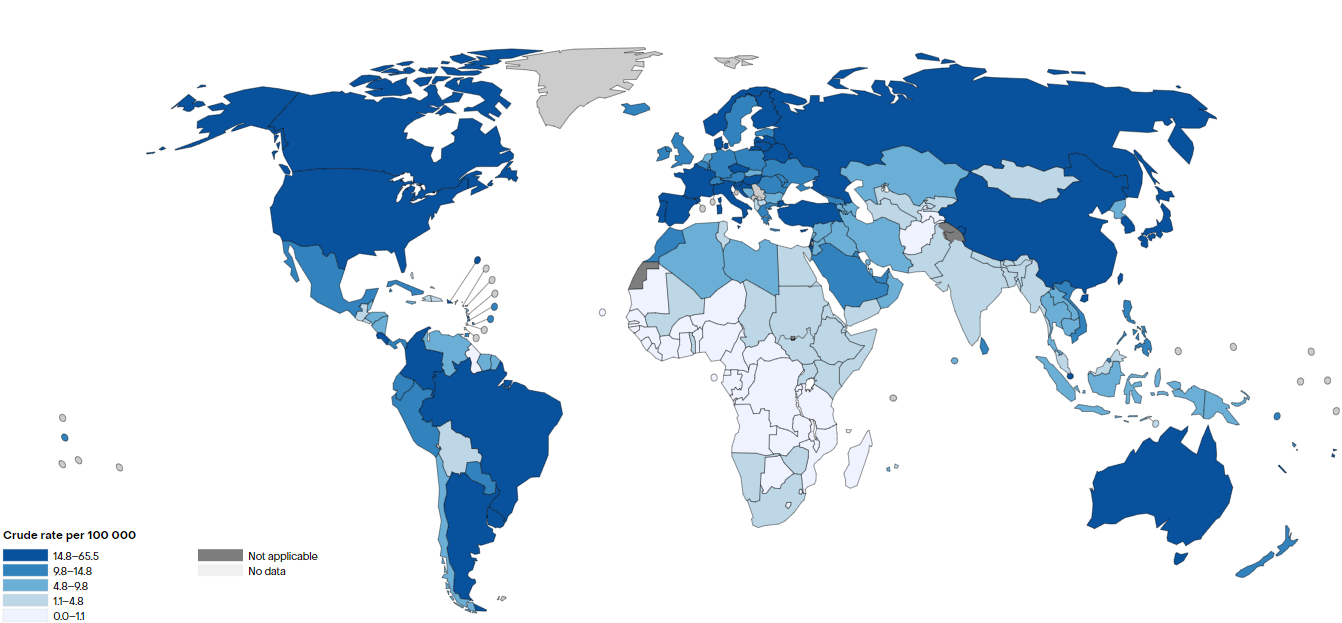
\includegraphics[width=1.00 \textwidth]{1/figures/tb_inc_ct_mujeres.png}
			\caption[Tasa bruta de incidencia de cáncer de tiroides en mujeres por 100 000 personas]{Tasa bruta de incidencia de cáncer de tiroides en mujeres por 100 000 personas. \\
			Fuente: \cite{ws_oms2022cancert}. \textit{Cancer Today}.}
			\label{1:fig}
		\end{center}
	\end{figure}


	\begin{figure}[H]
		\begin{center}
			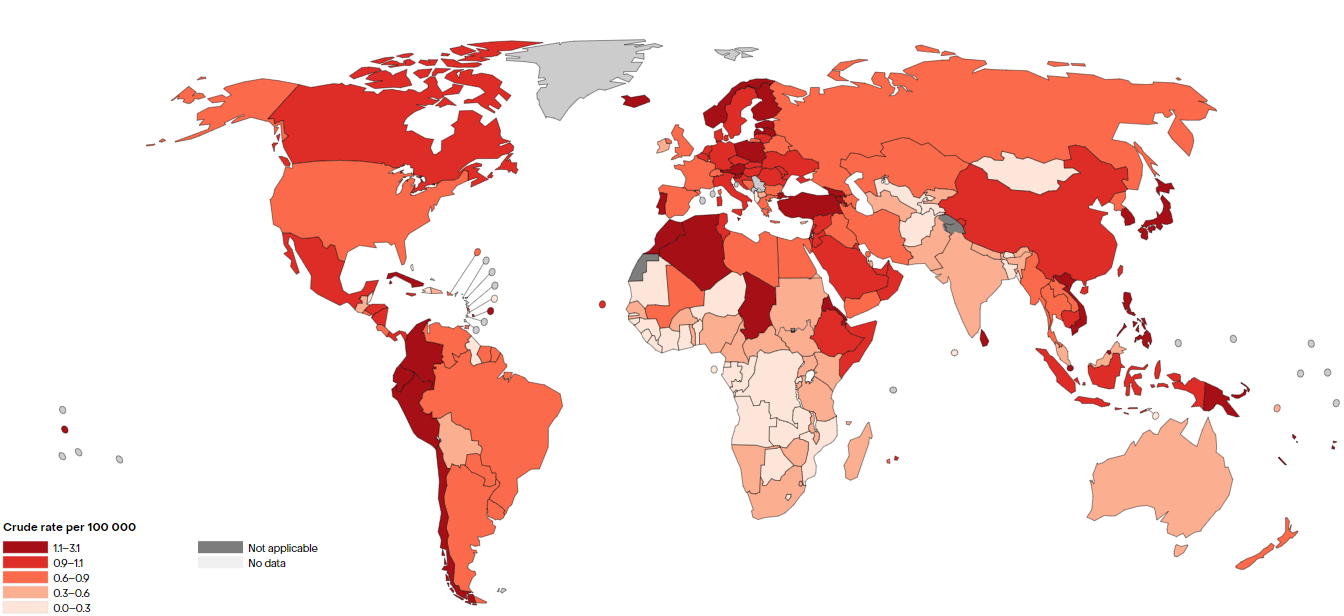
\includegraphics[width=1.00 \textwidth]{1/figures/tb_mor_ct_mujeres.png}
			\caption[Tasa bruta de mortalidad de cáncer de tiroides en mujeres por 100 000 personas]{Tasa bruta de mortalidad de cáncer de tiroides en mujeres por 100 000 personas. \\
			Fuente: \cite{ws_oms2022cancert}. \textit{Cancer Today}.}
			\label{1:fig2}
		\end{center}
	\end{figure}

	De igual forma, en el caso de los varones, el Perú también se encuentra entre los rangos más altos de incidencia y mortalidad. A continuación, se muestran estos datos en la Figura \ref{1:fig3} y Figura \ref{1:fig4}.

	\begin{figure}[H]
		\begin{center}
			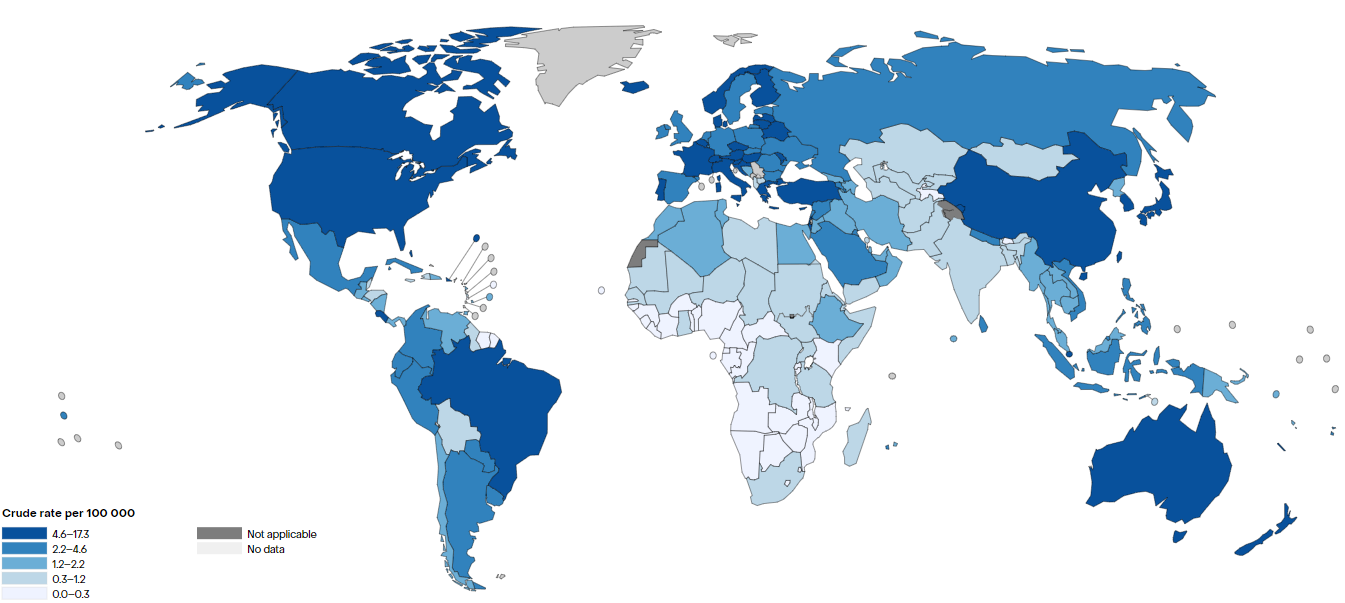
\includegraphics[width=1.00 \textwidth]{1/figures/tb_inc_ct_varones.png}
			\caption[Tasa bruta de incidencia de cáncer de tiroides en varones por 100 000 personas]{Tasa bruta de incidencia de cáncer de tiroides en varones por 100 000 personas. \\
			Fuente: \cite{ws_oms2022cancert}. \textit{Cancer Today}.}
			\label{1:fig3}
		\end{center}
	\end{figure}

	\begin{figure}[H]
		\begin{center}
			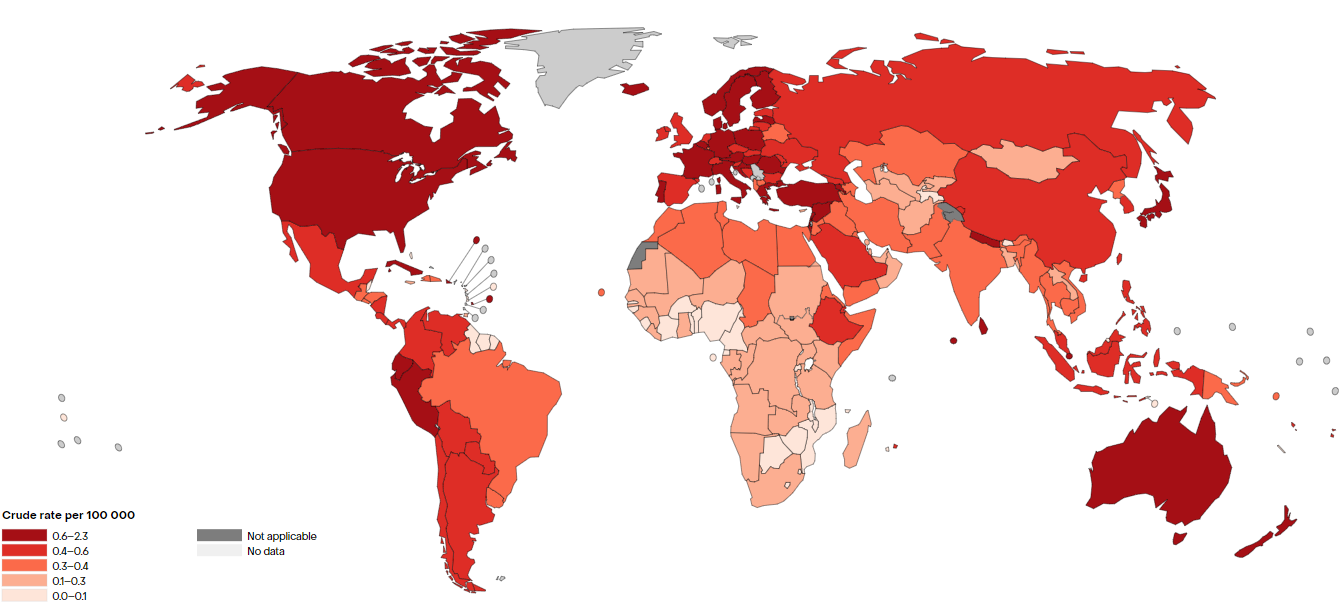
\includegraphics[width=1.00 \textwidth]{1/figures/tb_mor_ct_varones.png}
			\caption[Tasa bruta de mortalidad de cáncer de tiroides en varones por 100 000 personas]{Tasa bruta de mortalidad de cáncer de tiroides en varones por 100 000 personas. \\
			Fuente: \cite{ws_oms2022cancert}. \textit{Cancer Today}.}
			\label{1:fig4}
		\end{center}
	\end{figure}

	Con la Figura \ref{1:fig5} que muestra los mismos índices distribuidos por género y regiones del mundo, es fácil notar la alta incidencia de este tipo de cáncer en las mujeres, siendo la región con mayor incidencia América del Norte, mientras que la de mayor mortalidad es Oceanía. La región de Latino América y el Caribe supera a Norte América en mortalidad, aunque se encuentra por debajo de Oceanía y Europa.

	\begin{figure}[H]
		\begin{center}
			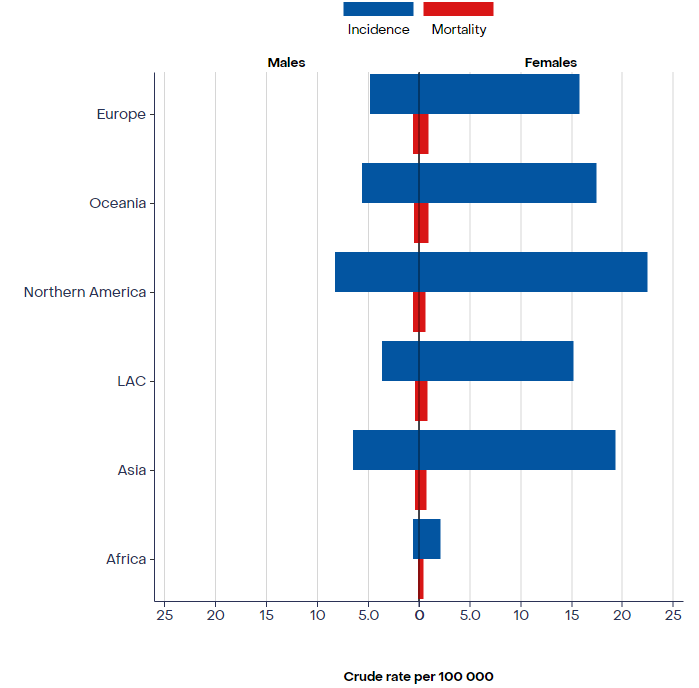
\includegraphics[width=0.60 \textwidth]{1/figures/tb_inc_mor_gen_y_reg.png}
			\caption[Tasa bruta de incidencia y mortalidad de cáncer de tiroides por género y región]{Tasa bruta de incidencia y mortalidad de cáncer de tiroides por género y región. \\
			Fuente: \cite{ws_oms2022cancert}. \textit{Cancer Today}.}
			\label{1:fig5}
		\end{center}
	\end{figure}
	\end{comment}
	El avance de la inteligencia artificial (IA) y la visión por computadora ofrecen la posibilidad de desarrollar sistemas de monitoreo automatizados que puedan detectar daños en tiempo real, optimizando el mantenimiento de las carreteras y disminuyendo los costos asociados a la rehabilitación vial.\parencite{pr_haugen2016amethy}.

	%Para la detección temprana de este tipo de cáncer o desarrollo de tumores, depende en gran medida de la experiencia y la capacidad cognitiva de un experto en radiología, y muchos de estos se ven en la necesidad de utilizar no muy avanzados sistemas de pre-diagnóstico por computadora, mejor conocido como CAD por sus siglas en inglés \parencite{pr_zhu2021agendlframew}. Ante grandes limitaciones de sistemas CAD básicos, y aprovechando el extenso uso de la Inteligencia Artificial, el Deep Learning y sus algoritmos son capaces de incorporar mayor eficacia a dichos sistemas.

	%El Deep Learning ha sido usado ampliamente como herramienta para el procesamiento de imágenes médicas, no solo para detectar diferentes tipos de cáncer o nódulos como los relacionados a los pulmones, sino también para la retinopatía diabética y localización de feto en ecografías, e inclusive en la detección del COVID-19 \parencite{pr_bhatta2021medimage}. Además, el aumento de la calidad de imágenes de ultrasonido que se fue desarrollando en los últimos 30 años, aumentando cada vez más resolución de las imágenes y reduciendo el tiempo de adquisición, ha permitido una mejora en términos de detección de enfermedad; sin embargo, aún se requiere de un médico especializado y debidamente entrenado para lograr un realizar un correcto análisis de las imágenes, por ello se vio en la necesidad de encontrar métodos de clasificación automatizada, pero dichos métodos antiguos consumían bastante tiempo, gran poder computacional y poca capacidad de generalización de resultados, es así que en este contexto, apareció una novedosa arquitectura de Deep Learning que actualmente es usado en diferentes áreas el día de hoy: las Redes Neuronales Convolucionales o CNN, quitando en gran medida los problemas de las antigua técnicas \parencite{pr_signgh20203ddl}. Sin embargo, es importante mencionar que estos últimos años han ido apareciendo nuevas arquitecturas capaces incluso de superar a los ya altamente difundidos CNN. Y es que a pesar del dominio actual de estas redes, las arquitecturas basadas en Transformer han ido tomando cada vez más mayor importancia dentro del mundo de la Inteligencia Artificial, y esto incluye también el área de procesamiento de imágenes médicas gracias a los Vision Transformers o ViT, una versión de los Transformers originales orientados al procesamiento de imágenes.
	
	%El desarrollo de estas nuevas tecnologías basadas en distintos algoritmos de Inteligencia Artificial, ya sea en CNN, ViT o incluso ambos, podrían mejorar aún más los tiempos de pre-diagnóstico de nódulos tiroideos y, además, aumentar los porcentajes de aciertos de los especialistas en estas tareas de diagnóstico a través de un trabajo conjunto con estas tecnologías de alto potencial.



	\section{Formulación del Problema}
	Con el objetivo de formular los objetivos de esta investigación, se propusieron las siguientes preguntas.
	\subsection{Problema General}
	PG: \newcommand{\ProblemaGeneral}{
	¿Cómo se podría detectar y gestionar de manera automatizada y eficiente el desgaste y deterioro de los pavimentos en Lima Metropolitana para reducir los costos de mantenimiento y mejorar la seguridad vial?
	}
	\ProblemaGeneral
	\subsection{Problemas Específicos}
	\newcommand{\Pbone}{
	¿Cómo podría implementarse un sistema automatizado para monitorear y clasificar en tiempo real el deterioro de los pavimentos?
	}
	\newcommand{\Pbtwo}{
	¿De qué manera podría reducirse el costo económico derivado de la rehabilitación tardía de carreteras en mal estado?
	}
	\newcommand{\Pbthree}{
	¿Cómo se podría minimizar el riesgo de accidentes de tránsito ocasionados por el mal estado de las vías urbanas?
	}
	\newcommand{\Pbfour}{
	¿Qué estrategias permitirían priorizar la reparación de las áreas más deterioradas para optimizar la distribución de los recursos?
	}

	\begin{itemize}
		\item PE1: {\Pbone}
		\item PE2: {\Pbtwo}
		\item PE3: {\Pbthree}
		\item PE4: {\Pbfour}
	\end{itemize}

	\section{Objetivos de la Investigación}
	A continuación, se presentan el objetivo general y los objetivos específicos.
	\subsection{Objetivo General}
	OG: \newcommand{\ObjetivoGeneral}{
	Desarrollar un modelo de clasificación automatizada utilizando redes neuronales convolucionales (CNN) para detectar y clasificar el deterioro de los pavimentos en Lima Metropolitana, optimizando el mantenimiento y mejorando la seguridad vial.
	}
	\ObjetivoGeneral
	\subsection{Objetivos Específicos}
	\newcommand{\Objone}{
	Implementar un sistema de monitoreo y clasificación basado en IA y visión por computadora para la identificación de grietas y baches en tiempo real.
	}
	\newcommand{\Objtwo}{
	Analizar el impacto económico de la detección temprana de daños en la infraestructura vial de Lima.
	}
	\newcommand{\Objthree}{
	Priorizar áreas críticas de deterioro para optimizar el uso de los recursos en las intervenciones de mantenimiento.
	}
	\newcommand{\Objfour}{
	Evaluar la precisión y eficiencia del modelo propuesto frente a métodos tradicionales de inspección vial.
	}

	\begin{itemize}
		\item OE1: {\Objone}
		\item OE2: {\Objtwo}
		\item OE3: {\Objthree}
		\item OE4: {\Objfour}
	\end{itemize}

	\section{Hipótesis}
	
	\subsection{Hipótesis General}
	La implementación de un modelo automatizado de clasificación de deterioros en pavimentos, basado en redes neuronales convolucionales, mejorará la detección y el mantenimiento de las vías en Lima Metropolitana, reduciendo costos y aumentando la seguridad vial.
	\subsection{Hipótesis Específicos}

	\newcommand{\Hione}{
	El uso de redes neuronales convolucionales permitirá una clasificación más precisa del estado de los pavimentos respecto a métodos tradicionales.}
	\newcommand{\Hitwo}{
	La detección automatizada y en tiempo real reducirá el tiempo de respuesta para las reparaciones, minimizando los costos a largo plazo.}
	\newcommand{\Hithree}{
	La priorización de las zonas más deterioradas mejorará la eficiencia en la asignación de recursos.}
	

	\begin{itemize}
		\item H1: {\Hione}
		\item H2: {\Hitwo}
		\item H3: {\Hithree}
	\end{itemize}


	\section{Justificación de la Investigación}

	\subsection{Teórica}
	La investigación aportará al campo de la inteligencia artificial aplicada a la infraestructura urbana, ampliando el conocimiento sobre el uso de redes neuronales convolucionales para la clasificación de imágenes en un contexto de mantenimiento vial.
	\subsection{Práctica}
	La implementación del sistema propuesto contribuirá a mejorar la gestión del mantenimiento de carreteras en Lima Metropolitana, reduciendo los costos asociados a reparaciones y mejorando la seguridad de los ciudadanos.
	\subsection{Metodológica}
	El estudio aplicará metodologías de redes neuronales convolucionales y técnicas de visión por computadora, lo que permitirá validar la efectividad de modelos de IA para tareas de clasificación en escenarios reales de infraestructura vial.
	\section{Delimitación del Estudio}
	A continuación, se presentará la delimitación espacial, temporal y conceptual.

	\subsection{Espacial}
	El estudio se llevará a cabo en las principales vías urbanas de Lima Metropolitana, donde se concentra el mayor flujo vehicular y deterioro de pavimentos.
	\subsection{Temporal}
	La investigación se desarrollará durante el período de 2024, con recolección de datos de campo y pruebas en un entorno controlado para evaluar el rendimiento del modelo propuesto.
	\subsection{Conceptual}
	El estudio se centrará en la aplicación de redes neuronales convolucionales para la clasificación de imágenes de pavimentos en estado de deterioro, considerando las variables clave de desgaste, como grietas y baches.
%\chapter{Marco Teórico}
\section{Antecedentes de la investigación}
En esta parte de la investigación se presentan algunos antecedentes relacionados a la detección y pre-diagnóstico de nódulos en distintos órganos y a través de diversas metodologías. Estos ayudarán a entender el enfoque y obtener bases para un correcto desarrollo del proyecto en cuestión.

\begin{comment}

\cite{pr_moreira2021deteclung} presenta una investigación relacionada a la elaboración de un sistema CAD (Computer-aided Detection) para la detección y segmentación de nódulos presentes en los pulmones.

Para realizar esta investigación, se tuvo en consideración la realidad que se atraviesa a nivel mundial sobre el cáncer de pulmón, y como este afecta a las personas sin importan su género, convirtiéndolo uno de los tipos de cáncer más mortales según la investigación mencionada. 

La presencia de nuevas formas de detectarlo como el uso de tomografías computarizadas tuvo un gran impacto para la detección temprana de los nódulos en estos órganos, ya que estos pueden significar un futuro desarrollo de cáncer. Sin embargo, realizar un análisis de este tipo de imágenes médicos no era nada trivial debido al complejo proceso de análisis con estas tecnologías. Ante esto, el Deep Learning apareció con una herramienta eficaz para ayudar a los médicos en el análisis de estas imágenes; sin embargo, pese a sus grandes ventajas, su aplicabilidad es muy limitada. Por tal motivo, esta tesis incluye modernos enfoques y técnicas para una detección automática de nódulos pulmonares.

De forma general, el algoritmo presentado en esta investigación consiste en dos bloques. El primero de estos se encarga de la detección de nódulo a través de técnicas de detección de objetos, mientras que el segundo se encarga de la segmentación de este. Los resultados obtenidos fueron del 79\% en recall; sin embargo, esto no fue suficiente para poder considerar al modelo como robusto, por ello, posteriormente, se utilizaron técnicas innovadoras en colaboración expertos en el área. Las anotaciones de los especialistas, junto con los resultados del sistema, mejoraron el desempeño general de la detección.

Para aumentar aún más las capacidades del sistema, se desarrolló en la parte final de la investigación un modelo de Deep Learning para la detección automática y la segmentación de nódulos pulmonares a través de imágenes tomográficas. Este también consistió en dos bloques, uno encargado de la segmentación automática y otro que corrige el anterior en base a dos puntos en los límites del nódulo. El modelo consiguió demostrar su capacidad para corregir la segmentación de nódulos pequeños, además de segmentar los nódulos no sólidos, los cuales presentaban un reto para el sistema.

\cite{pr_felgueiras20193dlungnod} reafirman la importancia de construir este tipo de sistemas mencionando al cáncer de pulmón como el principal tipo de cáncer en causar muertes en todo el mundo.

El sistema desarrollado en esta investigación fue basado en el diagnóstico a través de imágenes tomográficas que comúnmente es realizado por un médico experto; sin embargo, se menciona que este análisis siempre está sujeto a errores ya que existe mucha subjetividad en este tipo de diagnóstico, lo que conlleva muchas veces errores de detección. Además de la existencia de la tendencia al rechazo hacia esto tipo de sistemas CADx (Computer-aided Diagnosis) por parte de los médicos, esto debido a la fata de comprensión del cómo se realiza este tipo de pre-diagnóstico.

Para afrontar esta desconfianza a este tipo de sistemas, se menciona la existencia del Deep Hierarchical Semantic Convolutional Neural Network (HSCNN) que añadía a la capacidad de predecir si un nódulo era maligno o benigno, la función de otorgar evidencia visual del pre-diagnóstico a través de la predicción de las características del nódulo. Sin embargo, el conjunto de datos usado en esta investigación difería de las evaluaciones de los propios médicos. Por tal motivo, en la presente investigación se puso como un objetivo probar si la disminución de esta varianza en los datos podría mejorar los resultados del modelo HSCNN.

A través de un análisis de los datos, se logró mejorar la descripción de características. Este nuevo conjunto de datos fue revisado por especialista para comprobar su validez antes de ser ingresado al modelo HSCNN para predecir si un nódulo era maligno o benigno. Este proceso se hizo a través de un k-folds igual a 4 junto con cross-validation.

Los resultados fueron comparados con el modelo inicial, y se obtuvo que el nuevo HSCNN era mejor solo cuando se trataba de predecir si un nódulo era maligno. Las métricas del nuevo modelo fueron de 0.78 en accuracy, el AUC de la curva ROC es de 0.74, una sensibilidad 0.83 y una especificidad de 0.89, frente a las métricas de modelo original que obtuvo un accuracy de 0.84, un AUC de la curva ROC de 0.86, sensibilidad de 0.71 y una especificidad de 0.89. Esto significó que el modelo se equivocaba más cuando los nódulos a analizar eran pequeños. En general, los resultados distaron de los propios del modelo inicial, esto es debido a la reducción considerable de imágenes del conjunto de datos original. 

\cite{pr_supanta2021desalgdetec} menciona la incidencia de cáncer de pulmón en el Perú en el periodo 2010-2012 con un gran número de 3 121 casos diagnosticados, convirtiéndolo en el tercer tipo de cáncer más común en el país, y ocupa el segundo lugar en mortalidad con un número de 2 591 de muertes en el mismo periodo, esto debido al tardío diagnóstico de este mal. Por este motivo, es obvia la necesidad de realizar un examen de detección temprana donde es posible un tratamiento y, posteriormente, una posible cura a esta enfermedad. 

La investigación presenta una forma de realizar detección de nódulos pulmonares a través de imágenes radiográficas digitales que comúnmente presentan problemas como baja claridad y resaltado de las características, por ende, generan dificultades para realizar un correcto análisis de este tipo de imágenes. Las técnicas usadas son corrección gamma, análisis de proyecciones, erosión, filtros geométricos, dilatación, filtro de convergencia y la umbralización por el método Otsu, esto aplicado a un conjunto de datos de 50 radiografías de tórax.

Los resultamos muestran una sensibilidad del 0.91, especificidad de 0.96 y precisión de 0.94. 

Otra investigación relacionada a detectar alguna enfermedad a través de técnicas de Deep Learning y visión por computadora es la presentada por \cite{pr_monroy2021disvc} donde toma a la enfermedad de Parkinson como mal a detectar, esto a través del análisis de la escritura de una persona. Para tal objetivo, en la investigación se desarrolló un modelo de visión computacional para el pre-diagnóstico de esta enfermedad.

La metodología empieza con la adquisición y preprocesamiento de los datos, para posteriormente usar técnicas de extracción de características como SIFT, SURF, ORB y HOG. Estos serán ingresados a un modelo de Machine Learning (SVM, RF, KNN) que finalmente realizará una clasificación. Además, se usaron diferente arquitectura de Redes Neuronales Convolucionales como Inception, VGG16, VGG19, LeNet y ResNet50.

Los resultados finales fueron un 0.99 en accuracy, 0.99 en precisión, 0.99 en recall, 0.98 en F1-score y AUC.

\cite{pr_kang2022thysegclass} muestran la frecuencia de nódulos tiroideos en los diagnósticos, estando presente en el rango de 19\% y 68\% de todos los casos clínicos recopilados de personas adultas. El cáncer de tiroides es el número 9 en incidencia, mientras que es el número 6 en mortalidad, esto a nivel mundial según datos del 2018.

Se menciona que es importante tener métodos menos invasivos para determinar el cáncer de tiroides, teniendo en cuenta además que es necesario la detección a tiempo, pues esto aumenta la probabilidad de ser curado. El análisis de imágenes de ultrasonido es una buena opción a el análisis de, por ejemplo, cirugías. Sin embargo, esta forma de diagnóstico depende mucho de la experiencia del médico especialista, lo cual vuelve a este tipo de análisis muy subjetivo.

La segmentación y clasificación son herramientas claves dentro de un sistema de diagnóstico asistido, siendo ambos muy relacionados entre sí, pues comparten ciertas características de las imágenes (bordes de las imágenes pueden ser usados para la clasificación y segmentación). Afrontar ambas tareas al mismo tiempo en un solo modelo podría ser más robusto.

La red MTL propuesta en uno de los antecedentes es similar a una red de segmentación multiclases que genera como salida mapa de segmentación y predicciones categóricas.

La investigación presentada en este antecedente se centra también en una red MTL que también realizará procesos de segmentación y clasificación.

La metodología empieza con la data. Esta fue recolectada del West China Hospital. Se tuvieron 4 493 imágenes de ultrasonido, cada uno de un paciente. En específico, 2 576 imágenes pertenecen a nódulos benignos, mientras que 1 917 son malignos. Las anotaciones fueron verificadas por especialistas.

Para la evaluación de la clasificación se usó el accuracy, f1-score, ROC, área bajo la curva ROC (AUC). En el caso de la segmentación, se usó Dice coefficient y Intersection of Union (IoU).

Además, se definieron 3 medidas para cuantificar la inconsistencia al nivel de las tareas. El primero de estos evalúa a la clasificación, el segundo por la tarea de segmentación de segunda clase, y el tercero es para la segmentación de tercera clase.

El modelo construido en esta investigación se basó en MSL (Multi Stage Learning) y MTL (Multi Task Learning). Se diseño una red MS-MTL. Además, se determinó diferentes tipos de consistencia de tareas: intra e inter task consistency.

Los resultados fueron extraídos de 3 modelos CIsNet, MS-MTL y MS-MTL con intra e inter task consistency. La medida AUC obtenida para cada modelo es 0.9277, 0.9523 y 0.9608, respectivamente. Además, se determinó que el intra task cosistency y el MSL aumenta el desempeño de la segmentación. El caso de inter task consistency con MTL mejora el desempeño de las tareas de clasificación y segmentación. Con la combinación de ambas tareas de consistencias también se demuestra su efectividad.

El método usado en esta investigación se muestra en la Figura \ref{2:fig101}.

\begin{figure}[H]
	\begin{center}
		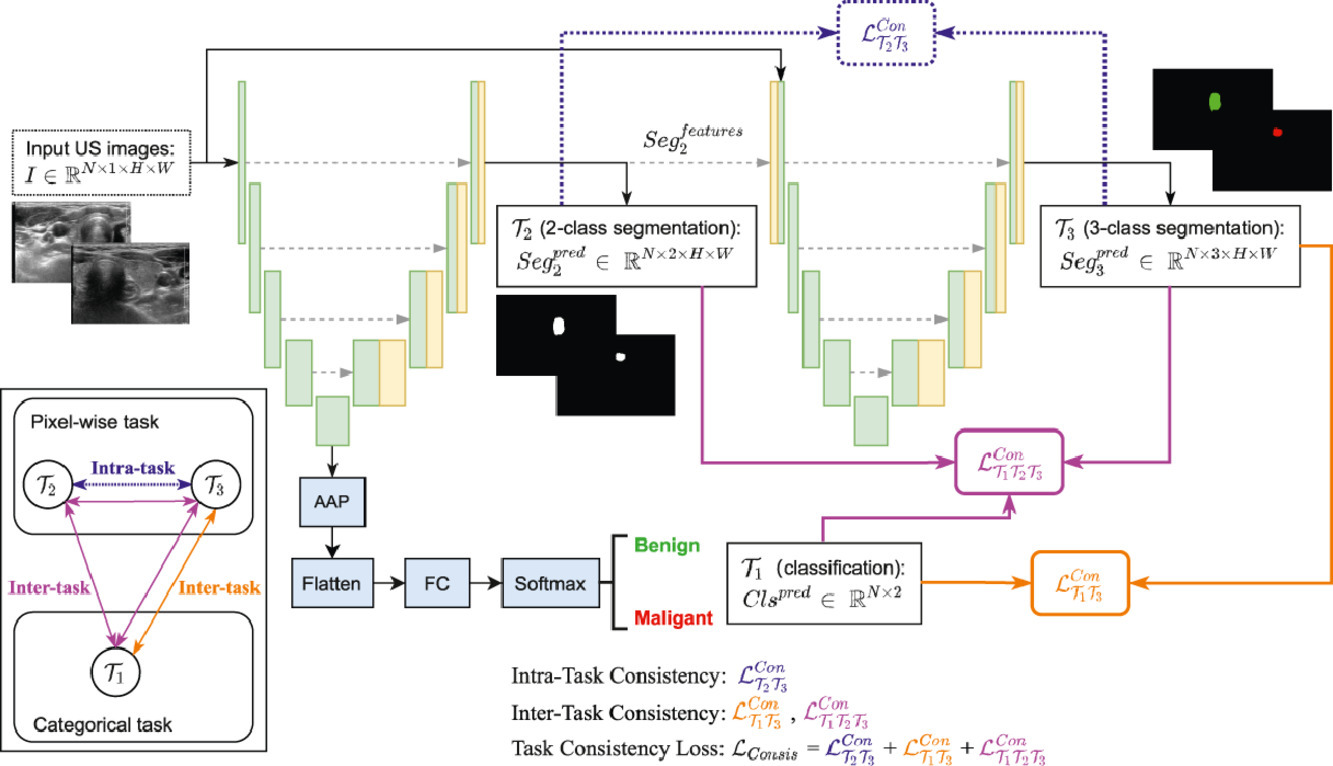
\includegraphics[width=1.00\textwidth]{2/figures/antecedente_4.jpg}
		\caption[Representación del método desarrollado]{Representación del método desarrollado. \\
		Fuente: \cite{pr_kang2022thysegclass}. \textit{Thyroid nodule segmentation and classification in ultrasound images through intra- and inter-task consistent learning}.}
		\label{2:fig101}
	\end{center}
\end{figure}


\cite{pr_sun2023classthynvit} presenta el problema de clasificar nódulos tiroideos nivel 3 debido a pocas características representativas que diferencien a los nódulos benignos de nivel 3 con los nódulos malignos, esto conlleva a obtener bajas precisiones en el pre-diagnóstico. Ante esto, en el artículo se presenta un modelo clasificador de nódulos tiroideos con ViT (Vision-Transformer-based) y el contrast learning. Estas técnicas ayudaron a minimizar la distancia de características en nódulos de una misma clase, lo cual mejora la capacidad predictiva del modelo. Finalmente, en la fase de testeo del modelo se logró un accuracy de 0.869, mientras que las demás métricas indican la superioridad frente a otros modelos clásicos de Deep Learning que también son usados para clasificar.

En la Figura \ref{2:fig102} se presenta la arquitectura de Vison Transformer desarrollada.

\begin{figure}[H]
	\begin{center}
		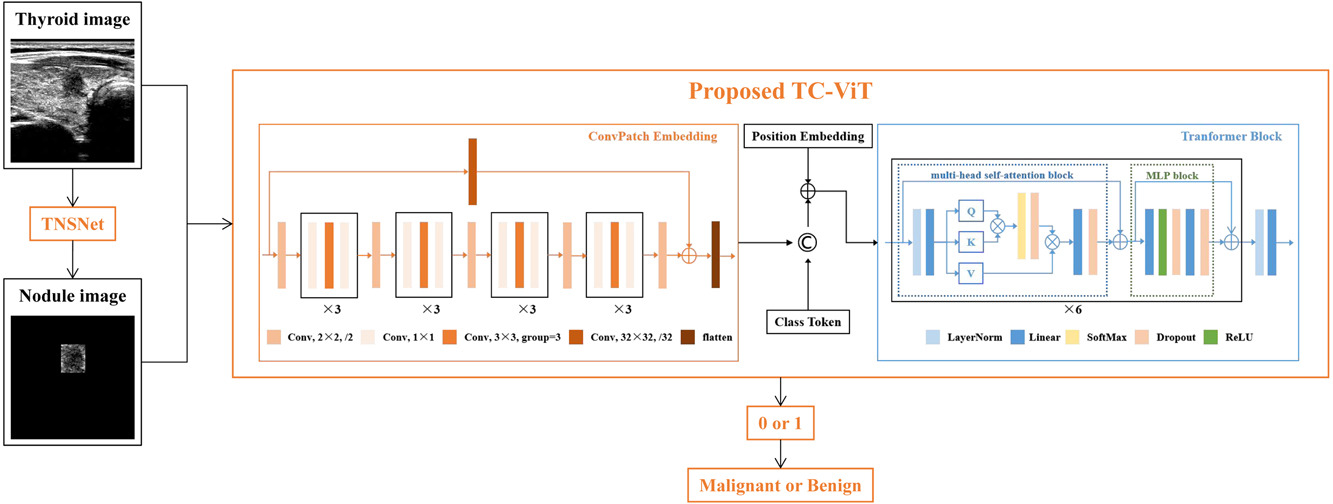
\includegraphics[width=1.00\textwidth]{2/figures/antecedente_5.jpg}
		\caption[Arquitectura de modelo TC-ViT]{Arquitectura de modelo TC-ViT. \\
		Fuente: \cite{pr_sun2023classthynvit}. \textit{Classification for thyroid nodule using ViT with contrastive learning in ultrasound images}.}
		\label{2:fig102}
	\end{center}
\end{figure}


\cite{pr_zhang2023madlap} presenta el nivel de importancia de poseer una buena base de datos etiquetada correctamente para lograr entrenar un buen modelo de Machine Learning. En este artículo se desarrolla y presenta a la herramienta Multistep Automated Data Labelling Procedure (MADLaP) que facilita y automatiza el proceso de etiquetado de datos relacionados a nódulos tiroideos. Este incluye el procesamiento de leguaje natural basado en reglas, el Deep Learning para segmentación de imágenes y el reconocimiento óptico de caracteres. MADLaP fue desarrollado en la fase de entrenamiento con datos de 378 pacientes, mientras que en la fase de prueba se usaron datos de 93. Este obtuvo finalmente un accuracy de 0.83.

\cite{pr_deng2022autclass} ponen al cáncer de tiroides como el que más ha prevalecido en las últimas 3 décadas. Existen diversos sistemas que ayudan a la detección de los nódulos en esta glándula; sin embargo, muchos de estos solo se limitan a determinar si un nódulo es maligno o benigno, y no muestran el porqué de la toma de esa decisión por parte del sistema, lo cual genera desconfianza entre los especialistas al momento de usarlos. Para afrontar esto, se desarrolla primeramente una estratificación de riesgo basada en el léxico estandarizado ACR TI-RADS. Posteriormente, se realiza la clasificación entre benigno y maligno. De formar general, el método realizará una caracterización del nódulo basado en ACR TI-RADS para detectar su nivel de riesgo y la clase al que pertenece (benigno o maligno). Los resultados muestran en la evaluación un accuracy de 0.9355, un sensitivity de 0.9386 y una specificity de 0.9314. 

Se realizó la notación de las imágenes de nódulos con los indicadores del diccionario de ACR TI-RADS. Para afrontar el desbalanceo de la data, se realizó un proceso de mejora de la data creando imágenes a través de giros, recortes y mezclas. Se extrajeron las áreas de interés de las imágenes a través de una red en cascada. Se quitaron las anotaciones manuales en las imágenes (limpieza de imagen). Una vez concluido con el procesamiento de las imágenes, se realizó la construcción y ejecución del modelo de Deep Learning Multi-Task Learning (MLT). Finalmente, el modelo obtenido fue comparado con otros a través de los siguientes indicadores: accuracy, sensitivity, specificity y el área bajo la curva. 

\cite{pr_wang2020autodiag} mencionan que los nódulos tiroideos son uno de los primeros síntomas que podrían conllevar a un cáncer en la tiroides. Este tipo de cáncer es uno de los que tiene mayor incidencia y que esta tendencia ha ido en crecimiento durando los últimos 30 años.

Además, se menciona que, para ayudar a esta detección, se han propuesto anteriormente varios sistemas de diagnóstico asistido; sin embargo, estos solo realizan dicho proceso a través de solo una imagen de ultrasonido en vez de usar todas aquellas que se obtienen de un examen. Por esto, en este artículo, se desarrolla un modelo de Deep Learning para el pre-diagnóstico de tiroides a través de varias imágenes de ultrasonido. Esto a través de una integración de todas las características de las imágenes realizadas en un examen. 

La base de datos usada fue construida, y se obtuvieron resultados perfectamente comparables con los resultados de los antecedentes revisados en este artículo.

La metodología consistía en la construcción de tres redes distintas: feature extraction network, attenntion-based feature aggregation network, classification network. Estas tres redes juntas forman el modelo objetivo desarrollado en este artículo.

En general, la metodología consistía en, primero, la construcción del conjunto de datos que se conforma de imágenes de ultrasonido procedentes de un hospital. Se recolectaron cerca de 7 800 imágenes de 1 046 exámenes de entre los años 2015 y 2018. En segundos lugar, se realizó el etiquetado de los datos. Estas anotaciones se realizaron de acuerdo con los exámenes en general, y no a cada una de las imágenes que la conforman. Luego, se realizó la separación de la data en entrenamiento, prueba y validación. En la parte final de experimentación, se realizó un preprocesamiento con Data Augmentation y se definió 100 épocas para la fase de entrenamiento. El modelo ganador de la fase de validación fue probado con la data de prueba. Las métricas usadas para la evaluación fueron el accuracy, sensitivity (true positive rate) y el área bajo la curva (AUC ROC).

La Figura \ref{2:fig103} muestra la arquitectura propuesta en esta investigación.

\begin{figure}[H]
	\begin{center}
		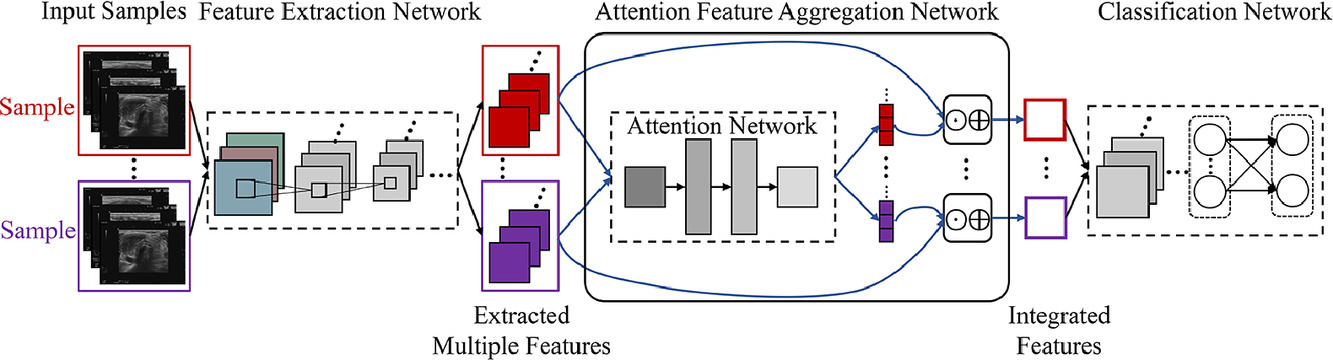
\includegraphics[width=1.00\textwidth]{2/figures/antecedente_8.jpg}
		\caption[Arquitecura de la red desarrollada]{Arquitecura de la red desarrollada. \\
		Fuente: \cite{pr_sun2023classthynvit}. \textit{Automatic diagnosis for thyroid nodules in ultrasound images by deep neural networks}.}
		\label{2:fig103}
	\end{center}
\end{figure}


\cite{pr_sun2022tnsnet} mencionan que, en el sistema endocrino, un problema muy común son los nódulos tiroideos. Normalmente estos pueden ser sólidos o de otras variadas texturas. La incidencia de esta enfermedad se ha ido incrementando a través de los años. Comúnmente se usan las imágenes de ultrasonido para detectar estos nódulos, esto lo hacen en tiempo real, tiene bajo costo y no es invasivo, por cual es una buena opción. Estas imágenes pueden otorgar información valiosa de los nódulos como los márgenes, ecogenicidad, calcificación, composición, etc. Además, existe el Thyroid Image Reporting y el sistema de datos TI-RADS que pueden cuantificar las características otorgadas por las imágenes de ultrasonido y evaluar si es benigno o maligno. Sin embargo, estas imágenes pueden traer problemas como bajo contraste y ruido de moteado, lo cual genera retos para extraer sus características. Este problema puede superarse a través de una correcta segmentación de los nódulos tiroideos. Así, la segmentación es un paso importante para realizar un pre-diagnóstico correcto. Esto puede ser aplicado a la evaluación automática en TI-RADS para facilitar la clasificación de los nódulos. Se añadió un shape-supervised path para mejorar la identificación de la forma, y así lograr una mejor segmentación.

La data que usaron se obtuvo de diversos escáneres disponibles comercialmente, juntando 3 786 imágenes de ultrasonido de nódulos tiroideos. Posteriormente, se realiza un preprocesamiento para estandarizar la data. Se realizó un proceso de limpieza de las imágenes para quitar los datos privados de los pacientes, y borrar imágenes erróneas. Se propuso TNSNet para asegurar una mejor detección y segmentación. Este modelo es un dual-path network que contiene dos partes region path y shape path. Ambos caminos se enfocan en las características de bordes y texturas (cada uno de estos para cada camino).

Se diseñó un dual-path loss function para el entramiento de ambos caminos del modelo. Para el camino de región, se usó el binary cross-entropy loss y el generalized Dice loss, ambos para entrenar la región de segmentación de los nódulos tiroideos. En el caso del segundo camino (camino de la forma) se combinó el Hausdoff distance loss y un modificado active contour loss. Esto fue construido para el entrenamiento del contorno de segmentación.

Las métricas usadas para evaluar la segmentación del modelo son Dice simialrity coefficient (DSC), sensitivity, specificity y el accuracy.

Los resultados muestran que en el caso de los nódulos benignos todos los modelos (el construido en el artículo y los de referencia) logran buenos resultados, esto debido a la buena calidad de las imágenes. En el caso de los nódulos malignos, el modelo TNSNet superó por completo a los otros modelos de referencia. Hubo otros experimentos, en los cuales, el modelo presentado en este artículo, de manera general, obtuvo mejores resultados.

La investigación realizada por \cite{pr_yang2023novelViTscc} se centra en la problemática del cáncer de piel, específicamente en el grave problema de los melanomas y la alta necesidad de una detección temprana para mejorar las posibilidades de supervivencia de los pacientes con este mal.

Además, se menciona que aunque la técnica más usada para la detección de melanomas es la dermatoscopia, su precisión es muy variada dependiendo el tipo de cáncer de piel con el que se está tratando. En este contexto, las técnicas de Deep Learning han demostrado ser un herramienta capaz de mejorar la precisión en las tareas relacionadas a clasificar el cáncer de piel, incluso superando al desempeño de los propios dermatólogos.

A pesar de estos logros del desarrollo de Deep Learning en esta área, se menciona que aún hay dificultad para la clasificación de algunos tipos de cáncer de piel como el melanoma. Por este motivo se propone una nueva arquitectura de red basada en los transformadores con el objetivo de mejorar la capacidad de los algoritmos de clasificación de cáncer de piel.

La metodología seguida por los autores inicia con la preparación de los datos. En este caso se usó el conjunto de datos HAM10000 que consta de 7 clases distintas de cáncer de piel. Las imágenes tuvieron que ser redimensionadas para los 4 distintos modelos a entrenar: Inception ResNet con Soft Attention (IRv2 + SA), ResNet50 con Soft Attention (ResNet50 + SA), ViTfSCD-Large y ViTfSCD-Base. Los parámetros de estos dos últimos modelos se muestran en la siguiente figura.

Además, se aplicó a las imágenes una limpieza, eliminando los duplicados. También pasó por un proceso de balanceo de las clases donde se intentó igualar la cantidad de imágenes en cada una de estas. Se realizó el proceso de Aumento de Datos a través de modificaciones en las imágenes como alterar la saturación de forma aleatoria, cambiar el contraste y el brillo. Finalmente, se definió los porcentajes de división para el conjunto de datos, siendo 85\% para el entrenamiento y 15\% para la prueba. 

Para la evaluación de los modelos se utilizaron las métricas de accuracy, precision, recall (sensitivity), specificity y F1 score. Los resultados de evaluar su capacidad de clasificación de los 4 modelos se muestran en la Tabla \ref{2:table1}, Tabla \ref{2:table2}, Tabla \ref{2:table3} y Tabla \ref{2:table4}.

\begin{table}[H]
	\caption[Comparación de resultados de los modelos (precision)]{Comparación de resultados de los modelos (precision).}
	\label{2:table1}
	\centering
	\small
	\begin{tabular}{ccccc}
		\specialrule{.1em}{.05em}{.05em}
		\multirow{2}{3cm}{Tipo de cáncer de piel} & \multicolumn{4}{l}{Precision} \\
		{} &{IRv2+SA} & {ResNet50+SA} & {ViTfSCD-B} & {ViTfSCD-L} \\
		\specialrule{.1em}{.05em}{.05em}
		{AKIEC} & {0.81} & {0.67} & {0.82} & {0.66} \\
		{BCC} & {0.95} & {0.90} & {1.00} & {0.89} \\
		{BKL} & {0.73} & {0.72} & {0.81} & {0.86} \\
		{DF} & {0.62} & {0.62} & {0.67} & {0.60} \\
		{MEL} & {0.70} & {0.62} & {0.60} & {0.79} \\
		{NV} & {0.95} & {0.96} & {0.94} & {0.97} \\
		{VASC} & {0.91} & {0.83} & {0.83} & {1.00} \\
		\specialrule{.1em}{.05em}{.05em}
	\end{tabular}
	\begin{flushleft}	
		\small Fuente: \cite{pr_yang2023novelViTscc}. \textit{A Novel Vision Transformer Model for Skin Cancer Classification}.
	\end{flushleft}
\end{table}

\begin{table}[H]
	\caption[Comparación de resultados de los modelos (sensitivity)]{Comparación de resultados de los modelos (sensitivity).}
	\label{2:table2}
	\centering
	\small
	\begin{tabular}{ccccc}
		\specialrule{.1em}{.05em}{.05em}
		\multirow{2}{3cm}{Tipo de cáncer de piel} & \multicolumn{4}{l}{Sensitivity} \\
		{} &{IRv2+SA} & {ResNet50+SA} & {ViTfSCD-B} & {ViTfSCD-L} \\
		\specialrule{.1em}{.05em}{.05em}
		{AKIEC} & {0.57} & {0.52} & {0.61} & {0.83} \\
		{BCC} & {0.73} & {0.69} & {0.54} & {0.65} \\
		{BKL} & {0.79} & {0.70} & {0.65} & {0.76} \\
		{DF} & {0.83} & {0.83} & {1.00} & {1.00} \\
		{MEL} & {0.47} & {0.59} & {0.53} & {0.68} \\
		{NV} & {0.97} & {0.98} & {0.98} & {0.99} \\
		{VASC} & {1.00} & {1.00} & {1.00} & {1.00} \\
		\specialrule{.1em}{.05em}{.05em}
	\end{tabular}
	\begin{flushleft}	
		\small Fuente: \cite{pr_yang2023novelViTscc}. \textit{A Novel Vision Transformer Model for Skin Cancer Classification}.
	\end{flushleft}
\end{table}

\begin{table}[H]
	\caption[Comparación de resultados de los modelos (f1-score)]{Comparación de resultados de los modelos (f1-score).}
	\label{2:table3}
	\centering
	\small
	\begin{tabular}{ccccc}
		\specialrule{.1em}{.05em}{.05em}
		\multirow{2}{3cm}{Tipo de cáncer de piel} & \multicolumn{4}{l}{F1-score} \\
		{} &{IRv2+SA} & {ResNet50+SA} & {ViTfSCD-B} & {ViTfSCD-L} \\
		\specialrule{.1em}{.05em}{.05em}
		{AKIEC} & {0.67} & {0.59} & {0.70} & {0.73} \\
		{BCC} & {0.83} & {0.78} & {0.70} & {0.76} \\
		{BKL} & {0.76} & {0.71} & {0.72} & {0.81} \\
		{DF} & {0.71} & {0.71} & {0.80} & {0.75} \\
		{MEL} & {0.56} & {0.61} & {0.56} & {0.73} \\
		{NV} & {0.96} & {0.97} & {0.96} & {0.98} \\
		{VASC} & {0.95} & {0.91} & {0.91} & {1.00} \\
		\specialrule{.1em}{.05em}{.05em}
	\end{tabular}
	\begin{flushleft}	
		\small Fuente: \cite{pr_yang2023novelViTscc}. \textit{A Novel Vision Transformer Model for Skin Cancer Classification}.
	\end{flushleft}
\end{table}

\begin{table}[H]
	\caption[Comparación de resultados de los modelos (specificity)]{Comparación de resultados de los modelos (specificity).}
	\label{2:table4}
	\centering
	\small
	\begin{tabular}{ccccc}
		\specialrule{.1em}{.05em}{.05em}
		\multirow{2}{3cm}{Tipo de cáncer de piel} & \multicolumn{4}{l}{Specificity} \\
		{} &{IRv2+SA} & {ResNet50+SA} & {ViTfSCD-B} & {ViTfSCD-L} \\
		\specialrule{.1em}{.05em}{.05em}
		{AKIEC} & {1.00} & {0.99} & {1.00} & {0.99} \\
		{BCC} & {1.00} & {1.00} & {1.00} & {1.00} \\
		{BKL} & {0.98} & {0.98} & {0.99} & {0.99} \\
		{DF} & {1.00} & {1.00} & {1.00} & {1.00} \\
		{MEL} & {0.99} & {0.99} & {0.99} & {0.99} \\
		{NV} & {0.80} & {0.84} & {0.76} & {0.88} \\
		{VASC} & {1.00} & {1.00} & {1.00} & {1.00} \\
		\specialrule{.1em}{.05em}{.05em}
	\end{tabular}
	\begin{flushleft}	
		\small Fuente: \cite{pr_yang2023novelViTscc}. \textit{A Novel Vision Transformer Model for Skin Cancer Classification}.
	\end{flushleft}
\end{table}

De los resultados, se observó que el modelo ViTfSCD-Large obtuvo el más alto precision, recall, y F1 scores. Además, el mismo modelo obtuvo un accuracy de 94.1\%, siendo el valor más alto, mientras que el modelo ViTfSCD-Base obtuvo 91.4\%.

Finalmente, se realizó una comparación de los modelos a través de su accuracy. En esta última sección, se comparó con otros modelos del estado de arte desarrollados con el conjunto de datos HAM10000. El primero de estos, implementado en 2020 y denominado Efficient-Net logró un accuracy de 92.6\%. También, en el año 2021, se desarrolló un método semi supervisado para la clasificación de imágenes médicas que obtuvo un accuracy de 92.5\%. 

Para esta comparación final, también se consideraron los resultados originales de los modelos IRv2, IRv2 + SA, ResNet50 y ResNet50 + SA junto con los resultados obtenidos en esta investigación. Además, también se realizaron experimentos con los modelos ViT originales (ViT-Base 16 y ViT-Large 16). Los resultados finales presentados en la Tabla \ref{2:table5} muestran que los modelos ViTfSCD-Base y ViTSCD-Large son superiores a sus versiones originales.

\begin{table}[H]
	\caption[Comparación de resultados según accuracy con el conjunto de datos HAM10000]{Comparación de resultados según accuracy con el conjunto de datos HAM10000.}
	\label{2:table5}
	\centering
	\small
	\begin{tabular}{llm{3cm}m{3cm}}
		\specialrule{.1em}{.05em}{.05em}
		{Métodos} & {Año} & {Accuracy general en sus paper} & {Accuracy general en propios experimentos} \\
		\specialrule{.1em}{.05em}{.05em}
		{Loss balancing y ensemble} & {2020} & {92.6\%} & {-} \\
		{Semi-supervised} & {2021} & {92.54\%} & {-} \\
		{ResNet50} & {2021} & {90.5\%} & {-} \\
		{IRv2} & {2021} & {91.2\%} & {-} \\
		{ResNet50 con Soft Attention} & {2021} & {91.5\%} & {91.5\%} \\
		{Inception ResNet con Soft Attention} & {2021} & {93.4\%} & {91.9\%} \\
		{Vision Transformer (ViT)-Base16} & {2021} & {-} & {91.1\%} \\
		{ViT-Large16} & {2021} & {-} & {93.7\%} \\
		{ViT para detección de cáncer de piel-Base} & {2022} & {-} & {91.4\%} \\
		{ViT para detección de cáncer de piel-Largo} & {2022} & {-} & {94.1\%} \\
		\specialrule{.1em}{.05em}{.05em}
	\end{tabular}
	\begin{flushleft}	
		\small Fuente: \cite{pr_yang2023novelViTscc}. \textit{A Novel Vision Transformer Model for Skin Cancer Classification}.
	\end{flushleft}
\end{table}

También se realizaron experimentos con el conjunto de datos DERMOFIT que consta de imágenes de lesiones clínicas de la piel divididas en 10 clases distintas. Los resultados originales con este conjunto de datos muestran que el modelo ResNet50 tuvo mejor desempeño que el modelo de árbol de decisión y KNN. 

Los nuevos experimentos con este conjunto de datos se llevaron a cabo con los modelos ResNet50, IRv2 y ViTfSCD-Base. Los resultados presentados en la Tabla \ref{2:table6} muestran el desempeño superior del modelo ViTfSCD frente a los demás.

\begin{table}[H]
	\caption[Comparación de resultados según accuracy con el conjunto de datos DERMOFIT]{Comparación de resultados según accuracy con el conjunto de datos DERMOFIT.}
	\label{2:table6}
	\centering
	\small
	\begin{tabular}{m{6cm}lm{3cm}m{3cm}}
		\specialrule{.1em}{.05em}{.05em}
		{Métodos} & {Año} & {Accuracy general en sus paper} & {Accuracy general en propios experimentos} \\
		\specialrule{.1em}{.05em}{.05em}
		{Decision Tree} & {2020} & {78.1\%} & {-} \\
		{Flat ResNet50} & {2020} & {78.7\%} & {-} \\
		{ResNet50} & {2022} & {-} & {71.2\%} \\
		{Inception ResNet (IRv2)} & {2022} & {-} & {71.9\%} \\
		{IRv2 + Soft Attention} & {2022} & {-} & {75.0\%} \\
		{Vision Transformer para la detección de cáncer de piel-Base} & {2021} & {-} & {80.5\%} \\
		\specialrule{.1em}{.05em}{.05em}
	\end{tabular}
	\begin{flushleft}	
		\small Fuente: \cite{pr_yang2023novelViTscc}. \textit{A Novel Vision Transformer Model for Skin Cancer Classification}.
	\end{flushleft}
\end{table}

La investigación presentada por \cite{pr_ayana2023ViTtrasnferLMC} se enfoca en el cáncer más común de las mujeres en los Estados Unidos: el cáncer de mama. Se dice que la tasa de incidencia de este mal ha ido en aumento en 0.5\% cada año; sin embargo, la tasa de mortalidad ha caído a un 45\% considerando datos desde el año 1989 hasta el 2020, esto debido a las mejoras constantes de los tratamientos y a las detecciones a tiempo, siendo la mamografía una técnica crucial en este último.

A pesar del importante papel de las mamografías en la detección a tiempo del cáncer de mama, existen casos de diagnósticos erróneos que muchas veces conllevan a procedimientos y gastos innecesarios para un paciente.

Ante este problema, se dice que se han desarrollado diversos sistema de detección asistida por computadora o CAD por sus siglas en inglés que tiene el principal objetivo de reducir los errores en la detección de este cáncer. 

Existen varios tipos de sistema CAD. Algunos no usan la Inteligencia Artificial, mientras otros utilizan las técnicas altamente difundidas del Deep Learning. Específicamente los modelos basados en las Redes Neuronales Convolucionales (CNN) han sido consideradas como prometedoras para las tareas detección de tumores de mama, llevándolos incluso a ser capaces de reducir la probabilidad de error humano. Sin embargo, esta clase de modelos también tienen sus dificultades. 

Los modelos CNN son computacionalmente caros debido a la complejidad y cantidad de convoluciones que se realizan. Además, en el contexto del cáncer de mama, estos modelos tienen dificultades en la localización de tumores, y una alta necesidad en el pre procesamiento, pues es necesario mejorar la calidad y reducir el ruido de las imágenes.

Otro problema a considerar es la falta de conjuntos de datos para el análisis de imágenes médicas. Para abordar esto, es necesario aplicar Transfer Learning y el Aumento de Datos.

En esta investigación se desarrolló un modelo de Deep Learning basado en los Vision Transformers y el Transfer Learning para la detección de cáncer de mama a través de mamografías. Para lograr esto, primero se abordó el problema de desbalanceo de las dos clases (benigno y maligno) en el conjunto de datos de mamografías, posteriormente, se desarrolló un método de Transfer Learning basado en los Vision Transformer con el objetivo de mejorar las deficiencias de los métodos de Transfer Learning basados en CNN.

El conjunto de datos usado para entrenar y probar el modelo fue el Digital Database for Screening Mammography (DDSM). Este consiste (hasta el último acceso del 12 de septiembre del 2022) de 13 128 imágenes mamográficas de las cuales 5 970 son benignas y 7 158 son malignas. Esto presentaba un claro desbalance con un ratio de 0.65:0.35. Esta distribución entre las clases podría generar errores en la etapa de aprendizaje del modelo, por este motivo, se desarrolló un nuevo método para el balanceo de datos a través de la técnica de Aumento de Datos, específicamente, se aplicó variaciones en la fluctuaciones de color de las imágenes, correción gamma, giro horizontal, sal y pimientas, y afilado o sharpening. El objetivo fue balancear el conjunto de datos para realizar validación cruzada de 5 pliegues, para lograr esto, se dividió al conjunto de datos en 5 partes o pliegues. Para las primeras 4 partes, se colocaron 1 145 imágenes de tumores malignos en cada una, mientras que para el quinto pliegue se tenían  1 146. Además, en los primeros 4 pliegues se tuvieron 955 imágenes de tumores benignos, a la vez que en el quinto pliegue se tuvieron 956. Para el lograr el balanceo de clases, se sometió a  imágenes de tumores benignos al proceso de aumento de imágenes 5 veces, mientras que para al grupo de imágenes de tumores malignos solo se aplicó una vez. Así, finalmente se obtuvo 1 146 imágenes para ambas clases presentes en cada pliegue. Este proceso se muestra en la Figura \ref{2:fig108}.

\begin{figure}[H]
	\begin{center}
		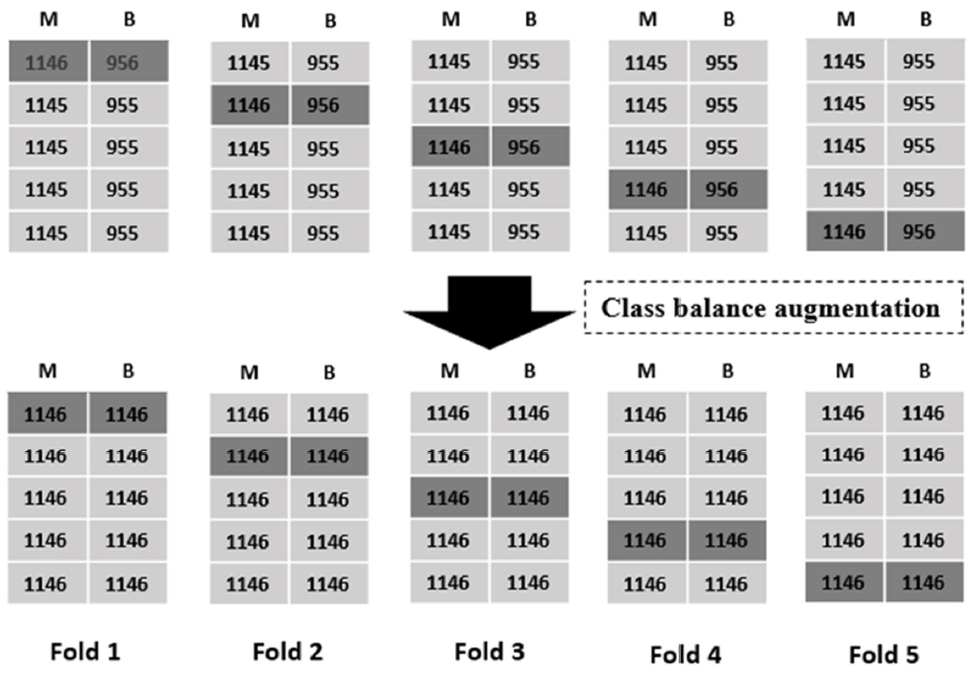
\includegraphics[width=0.90\textwidth]{2/figures/vitpaper2_part1.png}
		\caption[Balanceo de clases usando Aumento de Datos]{Balanceo de clases usando Aumento de Datos. \\
		Fuente: \cite{pr_ayana2023ViTtrasnferLMC}. \textit{Vision-Transformer-Based Transfer Learning for Mammogram Classification}.}
		\label{2:fig108}
	\end{center}
\end{figure}

Una vez obtenida la data ya balanceada, se realizó el preprocesamiento a las imágenes, específicamente, se redimensionó a las imágenes a 244 x 244 pixeles, esto debido a que el tamaño de las imágenes del conjunto de datos era variable. 

El diseño del modelo consiste inicialmente de la arquitectura de Vision Transformer. Se explica que siendo un modelo derivado de los convencionales transformer usados para el proceso del lenguaje natural o NLP donde las entradas son de una sola dimensión, los Vision Transformer se adaptaron para recibir entradas de dos dimensiones (imágenes). 

Específicamente, el modelo se encarga de dividir las entradas en pequeñas partes, también de dos dimensiones,conocidas como patches que finalmente servirán como entrada y serán pasada como word tokens, de igual forma que en un modelo transformer NLP. Aunque antes de proveer estos patches, se realizan los procesos de flattening, sequence imbedding, learnable embedding y patch embedding.

Además del bloque transformer, se tiene una parte de MLP encargada de la tarea de clasificación. Este posee una sola capa oculta y utiliza la función de activación GELU.

En el Figura \ref{2:fig109} se muestra la estructura del modelo implementado en la investigación.

\begin{figure}[H]
	\begin{center}
		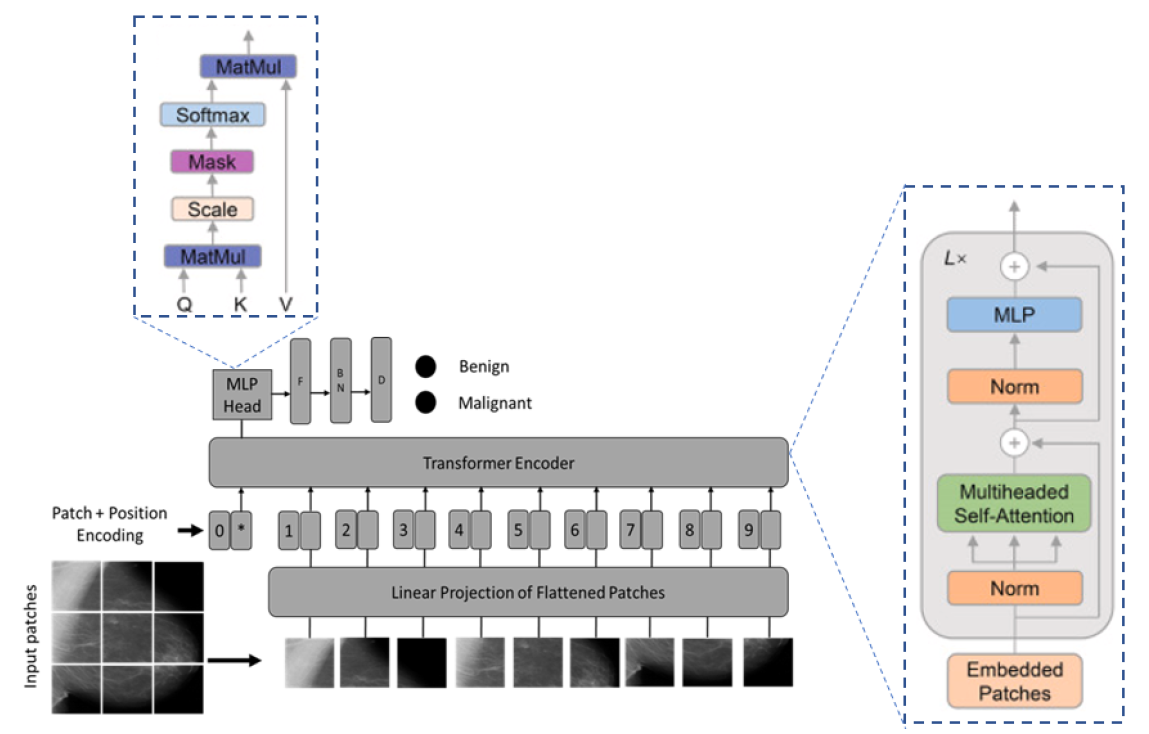
\includegraphics[width=1.00\textwidth]{2/figures/vitpaper2_part2.png}
		\caption[Estructura de ViT implementado]{Estructura de ViT implementado. \\
		Fuente: \cite{pr_ayana2023ViTtrasnferLMC}. \textit{Vision-Transformer-Based Transfer Learning for Mammogram Classification}.}
		\label{2:fig109}
	\end{center}
\end{figure}

El Transfer Learning fue aplicado en la investigación a través del uso de modelos de Vision Transformer pre-entrenados con el extenso conjunto de datos ImageNet, y posteriormente utilizados para entrenar el conjunto de datos de imágenes mamográficas. Es decir que se aprovechó el conocimiento de dichos modelos para la tarea final de clasificación de mamografías en benigno y maligno. Los modelos usados para este proceso fueron el Vision Transformer (ViT), Swin Transformer (Swin-T) y el Pyramid Vision Transformer (PVT).

El modelo Swin-T posee cuatro distintas versiones: Swin-base, Swin-tiny, Swin-small y Swin-large. Las variantes usadas en esta investigación fueron el Swin-small y Swin-base. Mientras que de las 4 versiones de PVT (PVT-tiny, PVT-small, PVT-medium y PVT-large), se usaron solo el PVT-medium y PVT-large.

Los modelos fueron entrenados con 50 épocas, una tasa de aprendizaje de 0.0001, optimizador Adam y un tamaño de lote de 64. Además, se dividió el conjunto de datos en 80\% para entrenamiento y 20\% para prueba.

Los Vision Transformer usaron GELU como función de activación, mientras que los CNN usaron ReLu. Ambos usaron el regularizador L2.

También se aplicó validación cruzada de 5 para lograr una mejor comparación en el rendimiento de los modelos.

Las métricas usadas para el proceso de evaluación de los modelos fueron el accuracy, AUC, F1-score, preicision, recall, el coeficiente de correlación de Matthew y el kappa score.

Se evaluó el método propuesto a través de 5 formas distintas: comparación de desempeño de los 3 modelos con Transfer Learning, comparación de los modelos Vision Transformer entrenados desde cero con el conjunto de datos de mamografías, comparación de Transfer Learning de Vision Transformer con los CNN, comparación de costo computacional de cada modelo Vision Transformer y, finalmente, se comparó el desempeño de los métodos desarrollados en esta investigación con otros que usaron el mismo conjunto de datos.

Como se muestra en la Tabla \ref{2:table7}, Tabla \ref{2:table8} y Tabla \ref{2:table9}, los 6 modelos Transfer Learning basados en arquitectura de Vision Transformer y entrenados con el conjunto de datos DDSM tuvieron un desempeño uniforme a través de todas la métricas.

\begin{table}[H]
	\caption[Resultado de los modelo ViT basados en Transfer Learning en el conjunto de datos DDSM (accuracy, AUC, f1-score)]{Resultado de los modelo ViT basados en Transfer Learning en el conjunto de datos DDSM (accuracy, AUC, f1-score).}
	\label{2:table7}
	\centering
	\small
	\begin{tabular}{m{3cm}m{3cm}m{2.4cm}m{2.5cm}m{2.5cm}}
		\specialrule{.1em}{.05em}{.05em}
		{Arquitectura} & {Modelo} & {Accuracy (95\%)} & {AUC (95\%)} & {F1 Score (95\%)}  \\
		\specialrule{.1em}{.05em}{.05em}
		\multirow{2}{3cm}{Vision Transformer} & {ViT-Base} & {$1 \pm 0$} & {$1 \pm 0$} & {$1 \pm 0$}  \\
		{} & {ViT-Large} & {$1 \pm 0$} & {$1 \pm 0$} & {$1 \pm 0$} \\
		\multirow{2}{3cm}{Swin Transformer} & {Swin-Small} & {$1 \pm 0$} & {$1 \pm 0$} & {$1 \pm 0$} \\
		{} & {Swim-Base} & {$1 \pm 0$} & {$1 \pm 0$} & {$1 \pm 0$} \\
		\multirow{2}{3cm}{Pyramid Vision Transformer} & {PVT-Medium} & {$1 \pm 0$} & {$1 \pm 0$} & {$1 \pm 0$} \\
		{} & {PVT-Large} & {$1 \pm 0$} & {$1 \pm 0$} & {$1 \pm 0$} \\
		\specialrule{.1em}{.05em}{.05em}
	\end{tabular}
	\begin{flushleft}	
		\small Fuente: \cite{pr_ayana2023ViTtrasnferLMC}. \textit{Vision-Transformer-Based Transfer Learning for Mammogram Classification}.
	\end{flushleft}
\end{table}

\begin{table}[H]
	\caption[Resultado de los modelo ViT basados en Transfer Learning en el conjunto de datos DDSM (precision, recall, MCC)]{Resultado de los modelo ViT basados en Transfer Learning en el conjunto de datos DDSM (precision, recall, MCC).}
	\label{2:table8}
	\centering
	\small
	\begin{tabular}{m{3cm}m{3cm}m{2.4cm}m{2.5cm}m{2.5cm}}
		\specialrule{.1em}{.05em}{.05em}
		{Arquitectura} & {Modelo} & {Precision (95\%)} & {Recall (95\%)} & {MCC (95\%)}  \\
		\specialrule{.1em}{.05em}{.05em}
		\multirow{2}{3cm}{Vision Transformer} & {ViT-Base} & {$1 \pm 0$} & {$1 \pm 0$} & {$1 \pm 0$}  \\
		{} & {ViT-Large} & {$1 \pm 0$} & {$1 \pm 0$} & {$1 \pm 0$} \\
		\multirow{2}{3cm}{Swin Transformer} & {Swin-Small} & {$1 \pm 0$} & {$1 \pm 0$} & {$1 \pm 0$} \\
		{} & {Swim-Base} & {$1 \pm 0$} & {$1 \pm 0$} & {$1 \pm 0$} \\
		\multirow{2}{3cm}{Pyramid Vision Transformer} & {PVT-Medium} & {$1 \pm 0$} & {$1 \pm 0$} & {$1 \pm 0$} \\
		{} & {PVT-Large} & {$1 \pm 0$} & {$1 \pm 0$} & {$1 \pm 0$} \\
		\specialrule{.1em}{.05em}{.05em}
	\end{tabular}
	\begin{flushleft}	
		\small Fuente: \cite{pr_ayana2023ViTtrasnferLMC}. \textit{Vision-Transformer-Based Transfer Learning for Mammogram Classification}.
	\end{flushleft}
\end{table}

\begin{table}[H]
	\caption[Resultado de los modelo ViT basados en Transfer Learning en el conjunto de datos DDSM (kappa)]{Resultado de los modelo ViT basados en Transfer Learning en el conjunto de datos DDSM (kappa).}
	\label{2:table9}
	\centering
	\small
	\begin{tabular}{m{3cm}m{3cm}m{2.4cm}}
		\specialrule{.1em}{.05em}{.05em}
		{Arquitectura} & {Modelo} & {Kappa (95\%)} \\
		\specialrule{.1em}{.05em}{.05em}
		\multirow{2}{3cm}{Vision Transformer} & {ViT-Base} & {$1 \pm 0$} \\
		{} & {ViT-Large} & {$1 \pm 0$} \\
		\multirow{2}{3cm}{Swin Transformer} & {Swin-Small} & {$1 \pm 0$}\\
		{} & {Swim-Base} & {$1 \pm 0$} \\
		\multirow{2}{3cm}{Pyramid Vision Transformer} & {PVT-Medium} & {$1 \pm 0$}\\
		{} & {PVT-Large} & {$1 \pm 0$}  \\
		\specialrule{.1em}{.05em}{.05em}
	\end{tabular}
	\begin{flushleft}	
		\small Fuente: \cite{pr_ayana2023ViTtrasnferLMC}. \textit{Vision-Transformer-Based Transfer Learning for Mammogram Classification}.
	\end{flushleft}
\end{table}

La Tabla \ref{2:table10}, Tabla \ref{2:table11} y Tabla \ref{2:table12} muestran los resultados de los modelos Vision Transformer inplementados desde cero y entrenados con el conjunto de datos DDSM.

\begin{table}[H]
	\caption[Resultado de los modelo ViT entrenados desde cero en el conjunto de datos DDSM (accuracy, AUC, f1-score)]{Resultado de los modelo ViT entrenados desde cero en el conjunto de datos DDSM (accuracy, AUC, f1-score).}
	\label{2:table10}
	\centering
	\small
	\begin{tabular}{m{3cm}m{3cm}m{2.4cm}m{2.5cm}m{2.5cm}}
		\specialrule{.1em}{.05em}{.05em}
		{Arquitectura} & {Modelo} & {Accuracy (95\%)} & {AUC (95\%)} & {F1 Score (95\%)}  \\
		\specialrule{.1em}{.05em}{.05em}
		\multirow{2}{3cm}{Vision Transformer} & {ViT-Base} & {$0.74 \pm 0.02$} & {$0.73 \pm 0.03$} & {$0.74 \pm 0.01$}  \\
		{} & {ViT-Large} & {$0.72 \pm 0.04$} & {$0.72 \pm 0.02$} & {$0.72 \pm 0.03$} \\
		\multirow{2}{3cm}{Swin Transformer} & {Swin-Small} & {$0.75 \pm 0.02$} & {$0.75 \pm 0.03$} & {$0.75 \pm 0.01$} \\
		{} & {Swim-Base} & {$0.76 \pm 0.01$} & {$0.75 \pm 0.02$} & {$0.75 \pm 0.02$} \\
		\multirow{2}{3cm}{Pyramid Vision Transformer} & {PVT-Medium} & {$0.78 \pm 0.02$} & {$0.77 \pm 0.02$} & {$0.78 \pm 0.01$} \\
		{} & {PVT-Large} & {$0.77 \pm 0.03$} & {$0.77 \pm 0.01$} & {$0.77 \pm 0.02$} \\
		\specialrule{.1em}{.05em}{.05em}
	\end{tabular}
	\begin{flushleft}	
		\small Fuente: \cite{pr_ayana2023ViTtrasnferLMC}. \textit{Vision-Transformer-Based Transfer Learning for Mammogram Classification}.
	\end{flushleft}
\end{table}

\begin{table}[H]
	\caption[Resultado de los modelo ViT entrenados desde cero en el conjunto de datos DDSM (precision, recall, MCC)]{Resultado de los modelo ViT entrenados desde cero en el conjunto de datos DDSM (precision, recall, MCC).}
	\label{2:table11}
	\centering
	\small
	\begin{tabular}{m{3cm}m{3cm}m{2.4cm}m{2.5cm}m{2.5cm}}
		\specialrule{.1em}{.05em}{.05em}
		{Arquitectura} & {Modelo} & {Precision (95\%)} & {Recall (95\%)} & {MCC (95\%)}  \\
		\specialrule{.1em}{.05em}{.05em}
		\multirow{2}{3cm}{Vision Transformer} & {ViT-Base} & {$0.74 \pm 0.01$} & {$0.74 \pm 0.01$} & {$0.73 \pm 0.03$}  \\
		{} & {ViT-Large} & {$0.72 \pm 0.04$} & {$0.72 \pm 0.03$} & {$0.71 \pm 0.02$} \\
		\multirow{2}{3cm}{Swin Transformer} & {Swin-Small} & {$0.75 \pm 0.02$} & {$0.75 \pm 0.02$} & {$0.74 \pm 0.03$} \\
		{} & {Swim-Base} & {$0.75 \pm 0.01$} & {$0.76 \pm 0.01$} & {$0.75 \pm 0.01$} \\
		\multirow{2}{3cm}{Pyramid Vision Transformer} & {PVT-Medium} & {$0.78 \pm 0.02$} & {$0.78 \pm 0.02$} & {$0.77 \pm 0.01$} \\
		{} & {PVT-Large} & {$0.77 \pm 0.02$} & {$0.77 \pm 0.02$} & {$0.77 \pm 0.01$} \\
		\specialrule{.1em}{.05em}{.05em}
	\end{tabular}
	\begin{flushleft}	
		\small Fuente: \cite{pr_ayana2023ViTtrasnferLMC}. \textit{Vision-Transformer-Based Transfer Learning for Mammogram Classification}.
	\end{flushleft}
\end{table}

\begin{table}[H]
	\caption[Resultado de los modelo ViT entrenados desde cero en el conjunto de datos DDSM (kappa)]{Resultado de los modelo ViT entrenados desde cero en el conjunto de datos DDSM (kappa).}
	\label{2:table12}
	\centering
	\small
	\begin{tabular}{m{3cm}m{3cm}m{2.4cm}}
		\specialrule{.1em}{.05em}{.05em}
		{Arquitectura} & {Modelo} & {Kappa (95\%)} \\
		\specialrule{.1em}{.05em}{.05em}
		\multirow{2}{3cm}{Vision Transformer} & {ViT-Base} & {$0.73 \pm 0.02$} \\
		{} & {ViT-Large} & {$0.72 \pm 0.01$} \\
		\multirow{2}{3cm}{Swin Transformer} & {Swin-Small} & {$0.74 \pm 0.02$}\\
		{} & {Swim-Base} & {$0.75 \pm 0.02$} \\
		\multirow{2}{3cm}{Pyramid Vision Transformer} & {PVT-Medium} & {$0.77 \pm 0.02$}\\
		{} & {PVT-Large} & {$0.77 \pm 0.01$}  \\
		\specialrule{.1em}{.05em}{.05em}
	\end{tabular}
	\begin{flushleft}	
		\small Fuente: \cite{pr_ayana2023ViTtrasnferLMC}. \textit{Vision-Transformer-Based Transfer Learning for Mammogram Classification}.
	\end{flushleft}
\end{table}

Se puede observar que el modelo PVT-medium obtuvo un mejor desempeño comparado a los demás modelos. Sin embargo, estos resultados se mantienen muy por debajo de los presentados anteriormente.

Finalmente, también se obtuvieron resultados de los experimentos de Transfer Learning con modelos CNN y el conjunto de datos DDSM. Estos se muestran en la Tabla \ref{2:table13}, Tabla \ref{2:table14} y Tabla \ref{2:table15}.

\begin{table}[H]
	\caption[Resultado de los modelos CNN basados en Transfer Learning en el conjunto de datos DDSM (accuracy, AUC, f1-score)]{Resultado de los modelos CNN basados en Transfer Learning en el conjunto de datos DDSM (accuracy, AUC, f1-score).}
	\label{2:table13}
	\centering
	\small
	\begin{tabular}{m{3cm}m{3cm}m{2.4cm}m{2.5cm}m{2.5cm}}
		\specialrule{.1em}{.05em}{.05em}
		{Arquitectura} & {Modelo} & {Accuracy (95\%)} & {AUC (95\%)} & {F1 Score (95\%)}  \\
		\specialrule{.1em}{.05em}{.05em}
		\multirow{2}{3cm}{ResNet} & {ResNet50} & {$0.95 \pm 0.01$} & {$0.96 \pm 0.01$} & {$0.95 \pm 0.01$}  \\
		{} & {ResNet101} & {$0.95 \pm 0.01$} & {$0.95 \pm 0.02$} & {$0.95 \pm 0.01$} \\
		\multirow{2}{3cm}{EfficientNet} & {EfficientNetB0} & {$0.94 \pm 0.02$} & {$0.94 \pm 0.01$} & {$0.94 \pm 0.01$} \\
		{} & {EfficientNetB2} & {$0.95 \pm 0.01$} & {$0.95 \pm 0.01$} & {$0.95 \pm 0.01$} \\
		\multirow{2}{3cm}{InceptionNet} & {InceptionNetV2} & {$0.93 \pm 0.02$} & {$0.93 \pm 0.01$} & {$0.93 \pm 0.02$} \\
		{} & {InceptionNetV3} & {$0.94 \pm 0.01$} & {$0.94 \pm 0.01$} & {$0.94 \pm 0.01$} \\
		\specialrule{.1em}{.05em}{.05em}
	\end{tabular}
	\begin{flushleft}	
		\small Fuente: \cite{pr_ayana2023ViTtrasnferLMC}. \textit{Vision-Transformer-Based Transfer Learning for Mammogram Classification}.
	\end{flushleft}
\end{table}

\begin{table}[H]
	\caption[Resultado de los modelos CNN basados en Transfer Learning en el conjunto de datos DDSM (precision, recall, MCC)]{Resultado de los modelos CNN basados en Transfer Learning en el conjunto de datos DDSM (precision, recall, MCC).}
	\label{2:table14}
	\centering
	\small
	\begin{tabular}{m{3cm}m{3cm}m{2.4cm}m{2.5cm}m{2.5cm}}
		\specialrule{.1em}{.05em}{.05em}
		{Arquitectura} & {Modelo} & {Precision (95\%)} & {Recall (95\%)} & {MCC (95\%)}  \\
		\specialrule{.1em}{.05em}{.05em}
		\multirow{2}{3cm}{ResNet} & {ResNet50} & {$0.95 \pm 0.01$} & {$0.95 \pm 0.01$} & {$0.94 \pm 0.01$}  \\
		{} & {ResNet101} & {$0.95 \pm 0.01$} & {$0.95 \pm 0.01$} & {$0.94 \pm 0.02$} \\
		\multirow{2}{3cm}{EfficientNet} & {EfficientNetB0} & {$0.94 \pm 0.01$} & {$0.94 \pm 0.01$} & {$0.93 \pm 0.03$} \\
		{} & {EfficientNetB2} & {$0.95 \pm 0.01$} & {$0.95 \pm 0.01$} & {$0.95 \pm 0.01$} \\
		\multirow{2}{3cm}{InceptionNet} & {InceptionNetV2} & {$0.93 \pm 0.02$} & {$0.93 \pm 0.02$} & {$0.93 \pm 0.03$} \\
		{} & {InceptionNetV3} & {$0.94 \pm 0.01$} & {$0.94 \pm 0.01$} & {$0.93 \pm 0.02$} \\
		\specialrule{.1em}{.05em}{.05em}
	\end{tabular}
	\begin{flushleft}	
		\small Fuente: \cite{pr_ayana2023ViTtrasnferLMC}. \textit{Vision-Transformer-Based Transfer Learning for Mammogram Classification}.
	\end{flushleft}
\end{table}

\begin{table}[H]
	\caption[Resultado de los modelos CNN basados en Transfer Learning en el conjunto de datos DDSM (kappa)]{Resultado de los modelos CNN basados en Transfer Learning en el conjunto de datos DDSM (kappa).}
	\label{2:table15}
	\centering
	\small
	\begin{tabular}{m{3cm}m{3cm}m{2.4cm}}
		\specialrule{.1em}{.05em}{.05em}
		{Arquitectura} & {Modelo} & {Kappa (95\%)} \\
		\specialrule{.1em}{.05em}{.05em}
		\multirow{2}{3cm}{ResNet} & {ResNet50} & {$0.94 \pm 0.02$} \\
		{} & {ResNet101} & {$0.94 \pm 0.02$} \\
		\multirow{2}{3cm}{EfficientNet} & {EfficientNetB0} & {$0.93 \pm 0.02$}\\
		{} & {EfficientNetB2} & {$0.95 \pm 0.01$} \\
		\multirow{2}{3cm}{InceptionNet} & {InceptionNetV2} & {$0.92 \pm 0.02$}\\
		{} & {InceptionNetV3} & {$0.93 \pm 0.02$}  \\
		\specialrule{.1em}{.05em}{.05em}
	\end{tabular}
	\begin{flushleft}	
		\small Fuente: \cite{pr_ayana2023ViTtrasnferLMC}. \textit{Vision-Transformer-Based Transfer Learning for Mammogram Classification}.
	\end{flushleft}
\end{table}


El desempeño de los modelos CNN también se encuentran por debajo de los Vision Transformer presentados inicialmente. 

\cite{pr_manzari2023MedViTGMIC} nos menciona que dentro del análisis de imágenes médicas, la tarea de clasificación es crucial. Por ello, este se ha visto beneficiado constantemente de novedosos sistemas de diagnóstico asistido, siendo los de mayor desempeño aquellos basados en Redes Neuronales Convolucionales (CNN), pues ofrecen predicciones cada vez más precisas incluso comparándose con los médicos. Sin embargo, estos también tienen algunas desventajas o dificultades, principalmente lo relacionado a su capacidad de aprendizaje de dependencias a largo alcance en conjuntos de datos visuales, esto debido al conocido sesgo local de las CNN.

En este contexto, las arquitecturas basadas en transformers y su mecanismo de autoatención, han demostrado ser capaces de solucionar estas desventajas de las CNN. Esto debido a su capacidad de modelar las dependencias a largo alcance de los datos, convirtiéndolos así en modelos superiores a las arquitectura de CNN, aunque con mayor necesidad en cantidad de datos de entrenamiento, recursos computacionales y tiempo.

A pesar de los beneficios que pueden traer las arquitecturas transformer frente a los CNN, estos están muy limitadas en su uso en las tareas de análisis de imágenes médicas. Esto es debido principalmente a sus desventajas ya mencionadas (alta necesidad de recursos computacionales y tiempo), pues en el entorno clínico, la eficiencia y la velocidad es de suma importancia para realizar pre-diagnósticos satisfactorios.

Los altos requerimientos de los transformer traen consigo grandes dificultades, impidiendo que estos puedan ser usados en situaciones clínicas reales. Además, también existe el problema de la suposición de una distribución similar en los datos que se van a ingresar al modelo; sin embargo, se sabe que esto no siempre se cumple en el entorno real, debido a que las imágenes médicas son capturadas a través de distintos dispositivos, diversos protocolos y diferentes lugares. Esta discrepancia en los datos puede generar que el rendimiento del modelo caiga considerablemente.

Ante este problema, la investigación propone un nueva arquitectura basada en transformer con capacidad de generalización de distintos tipos de imágenes médicas como las tomografías computarizadas, rayos X y ultrasonido. Su estructura se caracteriza por ser híbrida jerárquica, poseer patch embedding y poseer convoluciones y bloques de transformer. Además, se incluyó en la arquitectura del transformer un bloque de atención convolucional multi-cabezal con el fin de mejorar la capacidad de aprendizaje de representación local, incluso este permitió reducir la complejidad computacional comparado con un modelo transformer convencional.

Comparándolo con los CNN, el modelo desarrollado también demostró una capacidad superior en la tarea de predicción, al mismo tiempo que poseía menor complejidad.

De forma generar el modelo MedViT, propuesto en esta investigación, tiene como objetivo lograr una arquitectura híbrida capaz de desempeñarse en la tarea de clasificación de imágenes médicas, a través de la combinación de bloques de convolución y transformer, además de estar también compuesto por capas de path embedding, siguiendo así una tradicional arquitectura piramidal jerárquica.

Los bloques principales de modelo son el Efficient Convolution Block (ECB) y el Local Transformer Block (LTB). Estos se encargan de capturar las dependencias de los datos de entrada a largo y corto plazo.

También se propuso una nueva técnica de Aumento de Datos denominada Patch Momentum Charge (PMC) con el objetivo de mejorar el rendimiento del modelo.

Los experimentos se realizaron con 12 distintos conjuntos de datos de la categoría imágenes médicas. Todos estos se encontraron en MedMINIST, y conforman imágenes de tomografías computarizadas, rayos X, ultrasonido y tomografías de coherencia óptica (OCT). Esta variedad de datos permiten el entrenamiento de modelos en tareas de clasificación.

De forma específica, los conjuntos de datos usados fueron el PathMNIST (posee 100 000 image patches categorizadas en 9 clases distintas relacionadas a patologías en el colon), ChestMNIST (posee 112 120 imágenes frontales de rayos X de 32 717 pacientes dividida en 14 clases distintas de enfermedades de tórax), DermaMNIST (posee 10 015 imágenes dermatoscópicas recopiladas de distintas fuentes y divididas en 7 clases relacionadas a enfermedades de la piel), OCTMNIST (consta de 109 309 imágenes de OCT recopiladas de pacientes con enfermedades de la retina y dividida en 4 clases distintas), PneumoniaMNIST (recopila 5 856 imágenes radiográficas pediátricas de tórax categorizadas en 2 clases que indican presencia o no de neumonía), RetinaMNIST (provee 1 600 imágenes de fondo de retina de 628 pacientes y se divide en 5 clases que indican la gravedad de la enfermedad de retinopatía diabética), TissueMNIST (dividida en 8 clases, este conjunto de datos está compuesto de 236 386 imágenes segmentadas de tejidos de corteza renal), BloodMNIST (consta de 17 092 imágenes de células sanguíneas categorizadas en 8 clases), BreastMNIST (categorizada en las clases de benigno, maligno y normal, este conjunto de datos posee 780 ecografías mamarias) y OrganMNIST (consta de imágenes de tomografías computarizadas abdominales divididas en 11 clases en sus 3 versiones: Axial, Coronal y Sagital).

En la etapa de entrenamiento del modelo con los 12 conjuntos de datos descritos anteriormente, se siguieron los mismos ajustes de entrenamiento de MedMNISTv2. Se usaron 100 épocas con un tamaño de lote de 128 y se aplicó el redimensionado a las imágenes para obtener la forma de 224 x 224 pixeles. Además, se usó el optimizar AdamW con una tasa de aprendizaje de 0.0001.

MedViT consiste en 3 distintas arquitecturas definidas por su tamaño: MedViT-T, MedViT-S y MedViT-L. Estas fueron entrenadas de forma separada con cada uno de los conjuntos de datos. También se incluyó el Aumento de Datos a través de PMC.en la etapa de entrenamiento.

Las métricas usadas para evaluar las 3 versiones del modelo MedViT fueron el accuracy y la curva ROC. Esta elección fue debido a que el experimento se llevó a cabo en varios conjuntos de datos distintos entre sí. 

De los resultados mostrados en la Tabla \ref{2:table16}, Tabla \ref{2:table17}, Tabla \ref{2:table18} y Tabla \ref{2:table19}, los modelos MedViT superan, de forma general, en gran medida a los modelos basados en CNN en la misma tarea. Esto lleva a concluir que el modelo demuestra una alta capacidad de generalización en imágenes médicas.

\begin{table}[H]
	\caption[Comparación de resultados de los modelos MedViT con los CNN y AutoML (PathMNIST, ChestMNIST y DermaMNIST)]{Comparación de resultados de los modelos MedViT con los CNN y AutoML (PathMNIST, ChestMNIST y DermaMNIST).}
	\label{2:table16}
	\centering
	\small
	\begin{tabular}{lcccccc}
		\specialrule{.1em}{.05em}{.05em}
		\multirow{2}{3cm}{Métodos} & \multicolumn{2}{l}{PathMNIST} & \multicolumn{2}{l}{ChestMNIST} & \multicolumn{2}{l}{DermaMNIST} \\
		{} & {AUC} & {ACC} & {AUC} & {ACC} & {AUC} & {ACC} \\
		\specialrule{.1em}{.05em}{.05em}
		{ResNet-18 (28)} & {0.983} & {0.907} & {0.768} & {0.947} & {0.917} & {0.735} \\
		{RestNet-18 (224)} & {0.989} & {0.909} & {0.773} & {0.947} & {0.920} & {0.754} \\
		{ResNet-50 (28)} & {0.990} & {0.911} & {0.769} & {0.947} & {0.913} & {0.735} \\
		{RestNet-50 (224)} & {0.989} & {0.892} & {0.773} & {0.948} & {0.912} & {0.731} \\
		{auto-sklearn} & {0.934} & {0.716} & {0.649} & {0.779} & {0.902} & {0.719} \\
		{AutoKeras} & {0.959} & {0.834} & {0.742} & {0.937} & {0.915} & {0.749} \\
		{Google AutoML} & {0.944} & {0.728} & {0.778} & {0.948} & {0.914} & {0.768} \\
		{MedVIT-T (224)} & {0.994} & {0.938} & {0.786} & {0.956} & {0.914} & {0.768} \\
		{MedVIT-S (224)} & {0.993} & {0.942} & {0.791} & {0.954} & {0.937} & {0.780} \\
		{MedVIT-L (224)} & {0.984} & {0.933} & {0.805} & {0.959} & {0.920} & {0.773} \\
		\specialrule{.1em}{.05em}{.05em}
	\end{tabular}
	\begin{flushleft}	
		\small Fuente: \cite{pr_manzari2023MedViTGMIC}. \textit{MedViT: A robust vision transformer for generalized medical image classification}.
	\end{flushleft}
\end{table}

\begin{table}[H]
	\caption[Comparación de resultados de los modelos MedViT con los CNN y AutoML (OCTMNIST, PneumoniaMNIST y RetinaMNIST)]{Comparación de resultados de los modelos MedViT con los CNN y AutoML (OCTMNIST, PneumoniaMNIST y RetinaMNIST).}
	\label{2:table17}
	\centering
	\small
	\begin{tabular}{lcccccc}
		\specialrule{.1em}{.05em}{.05em}
		\multirow{2}{3cm}{Métodos} & \multicolumn{2}{l}{OCTMNIST} & \multicolumn{2}{l}{PneumoniaMNIST} & \multicolumn{2}{l}{RetinaMNIST} \\
		{} & {AUC} & {ACC} & {AUC} & {ACC} & {AUC} & {ACC} \\
		\specialrule{.1em}{.05em}{.05em}
		{ResNet-18 (28)} & {0.943} & {0.743} & {0.944} & {0.854} & {0.717} & {0.524} \\
		{RestNet-18 (224)} & {0.958} & {0.763} & {0.956} & {0.864} & {0.710} & {0.493} \\
		{ResNet-50 (28)} & {0.952} & {0.762} & {0.948} & {0.954} & {0.726} & {0.528} \\
		{RestNet-50 (224)} & {0.958} & {0.776} & {0.962} & {0.884} & {0.716} & {0.511} \\
		{auto-sklearn} & {0.887} & {0.601} & {0.942} & {0.855} & {0.690} & {0.515} \\
		{AutoKeras} & {0.955} & {0.763} & {0.947} & {0.878} & {0.719} & {0.503} \\
		{Google AutoML} & {0.963} & {0.771} & {0.991} & {0.946} & {0.750} & {0.531} \\
		{MedVIT-T (224)} & {0.961} & {0.767} & {0.993} & {0.949} & {0.752} & {0.534} \\
		{MedVIT-S (224)} & {0.960} & {0.982} & {0.995} & {0.961} & {0.773} & {0.561} \\
		{MedVIT-L (224)} & {0.945} & {0.761} & {0.991} & {0.921} & {0.754} & {0.552} \\
		\specialrule{.1em}{.05em}{.05em}
	\end{tabular}
	\begin{flushleft}	
		\small Fuente: \cite{pr_manzari2023MedViTGMIC}. \textit{MedViT: A robust vision transformer for generalized medical image classification}.
	\end{flushleft}
\end{table}

\begin{table}[H]
	\caption[Comparación de resultados de los modelos MedViT con los CNN y AutoML (BreastMNIST, BloodMNIST y TissueMNIST)]{Comparación de resultados de los modelos MedViT con los CNN y AutoML (BreastMNIST, BloodMNIST y TissueMNIST).}
	\label{2:table18}
	\centering
	\small
	\begin{tabular}{lcccccc}
		\specialrule{.1em}{.05em}{.05em}
		\multirow{2}{3cm}{Métodos} & \multicolumn{2}{l}{BreastMNIST} & \multicolumn{2}{l}{BloodMNIST} & \multicolumn{2}{l}{TissueMNIST} \\
		{} & {AUC} & {ACC} & {AUC} & {ACC} & {AUC} & {ACC} \\
		\specialrule{.1em}{.05em}{.05em}
		{ResNet-18 (28)} & {0.901} & {0.863} & {0.998} & {0.958} & {0.930} & {0.676} \\
		{RestNet-18 (224)} & {0.891} & {0.833} & {0.998} & {0.963} & {0.933} & {0.681} \\
		{ResNet-50 (28)} & {0.857} & {0.812} & {0.997} & {0.956} & {0.931} & {0.680} \\
		{RestNet-50 (224)} & {0.866} & {0.842} & {0.997} & {0.950} & {0.932} & {0.680} \\
		{auto-sklearn} & {0.836} & {0.803} & {0.984} & {0.878} & {0.828} & {0.532} \\
		{AutoKeras} & {0.871} & {0.831} & {0.998} & {0.961} & {0.941} & {0.703} \\
		{Google AutoML} & {0.919} & {0.861} & {0.998} & {0.966} & {0.924} & {0.673} \\
		{MedVIT-T (224)} & {0.934} & {0.896} & {0.996} & {0.950} & {0.943} & {0.703} \\
		{MedVIT-S (224)} & {0.938} & {0.897} & {0.997} & {0.951} & {0.952} & {0.731} \\
		{MedVIT-L (224)} & {0.929} & {0.883} & {0.996} & {0.954} & {0.935} & {0.699} \\
		\specialrule{.1em}{.05em}{.05em}
	\end{tabular}
	\begin{flushleft}	
		\small Fuente: \cite{pr_manzari2023MedViTGMIC}. \textit{MedViT: A robust vision transformer for generalized medical image classification}.
	\end{flushleft}
\end{table}

\begin{table}[H]
	\caption[Comparación de resultados de los modelos MedViT con los CNN y AutoML (OrganMNIST, OrganCMNIST y OrganSMNIST)]{Comparación de resultados de los modelos MedViT con los CNN y AutoML (OrganMNIST, OrganCMNIST y OrganSMNIST).}
	\label{2:table19}
	\centering
	\small
	\begin{tabular}{lcccccc}
		\specialrule{.1em}{.05em}{.05em}
		\multirow{2}{3cm}{Métodos} & \multicolumn{2}{l}{OrganMNIST} & \multicolumn{2}{l}{OrganCMNIST} & \multicolumn{2}{l}{OrganSMNIST} \\
		{} & {AUC} & {ACC} & {AUC} & {ACC} & {AUC} & {ACC} \\
		\specialrule{.1em}{.05em}{.05em}
		{ResNet-18 (28)} & {0.997} & {0.935} & {0.992} & {0.900} & {0.972} & {0.782} \\
		{RestNet-18 (224)} & {0.998} & {0.951} & {0.994} & {0.920} & {0.974} & {0.778} \\
		{ResNet-50 (28)} & {0.997} & {0.935} & {0.992} & {0.905} & {0.972} & {0.770} \\
		{RestNet-50 (224)} & {0.998} & {0.947} & {0.993} & {0.911} & {0.975} & {0.785} \\
		{auto-sklearn} & {0.963} & {0.762} & {0.976} & {0.829} & {0.845} & {0.672} \\
		{AutoKeras} & {0.994} & {0.905} & {0.990} & {0.879} & {0.974} & {0.813} \\
		{Google AutoML} & {0.990} & {0.886} & {0.988} & {0.877} & {0.964} & {0.749} \\
		{MedVIT-T (224)} & {0.995} & {0.931} & {0.991} & {0.901} & {0.972} & {0.789} \\
		{MedVIT-S (224)} & {0.996} & {0.928} & {0.993} & {0.916} & {0.987} & {0.805} \\
		{MedVIT-L (224)} & {0.997} & {0.943} & {0.994} & {0.922} & {0.973} & {0.806} \\
		\specialrule{.1em}{.05em}{.05em}
	\end{tabular}
	\begin{flushleft}	
		\small Fuente: \cite{pr_manzari2023MedViTGMIC}. \textit{MedViT: A robust vision transformer for generalized medical image classification}.
	\end{flushleft}
\end{table}

\cite{pr_regmi2023ViTChestXray} nos menciona la gran importancia que tiene el análisis de imágenes médicas para la detección a tiempo de enfermedades potencialmente mortales. Los radiólogos y personal clínico realizan esta importante tarea en la gran mayoría de los casos; sin embargo, sus interpretaciones de las imágenes no siempre están en lo correcto debido a que su análisis muchas veces está condicionado por el mismo observador, llevando a que los niveles de precisión para interpretar este tipo de datos no sean tan altos.

Esta tarea de interpretación de imágenes médicas es aun más importante en los casos de una alta necesidad de detectar a tiempo alguna enfermedad; por ejemplo, las relacionadas a los pulmones o las enfermedades gastrointestinales que pueden no causar daño como el reflujo ácido u otras de grave impacto como el cáncer de colon. Una detección a tiempo de estos permite aplicar los tratamientos debidos y así, consecuentemente, mejorar la calidad de vida de los pacientes. En este contexto, los sistemas de diagnóstico asistido por computadora (CAD por sus siglas en inglés) han demostrado ser de gran ayuda para los médicos y expertos clínicos en la tarea de realizar diagnósticos tempranos.

La capacidad de las Redes Neuronales Convolucionales (CNN) de poder adaptarse en detectar distintas característica de un conjunto de datos han permitido su desarrollo en el campo médico, específicamente en las tareas de segmentación, clasificación, registro y reconstrucción de imágenes médicas.

Otra técnica popular que va tomando cada vez más mayor importancia son los Vision Transformer (ViT) capaces también de desempeñarse satisfactoriamente en las tareas de clasificación de imágenes, a pesar de ser basados en los originales transformers especializados en tareas relacionadas a texto.

Otro tipo de arquitectura basada en transformer son los Data-Efficient Image Transformer (DeiT), una versión de nuevos de los ViT caracterizados por su baja dependencia a los datos a través de su enfoque maestro-estudiante.

En esta investigación se presentan distintas arquitecturas basadas en CNN y Transformer para la clasificación de radiografías de tórax en distintos tipos de enfermedades relacionadas. Específicamente, se usaron los modelos DeiT, ViT y Ensemble, este último basado en otros modelos CNN. También se aplicó Transfer Learning junto a modelos CNN previamente entrenados. Finalmente todos los modelos fueron comparados en la misma tarea de clasificación de imágenes.

Se usaron distintas versiones de ViT (ViT-B/16, ViT-L/16, ViT-L/32) pre-entrenados con el conjunto de datos ImageNet-21k. 

La diferencia principal entre ViT-L/16 y ViT-L/32 radica en el tamaño de los patch de entrada que permiten, siendo para el primer caso un patch de tamaño 16x16, mientras que el segundo un patch de 32 x 32. Todos estos modelos pasaron por un proceso de fine-tuning con 3 conjuntos de datos.

El primer conjunto de datos usado fue el Chest X-ray dataset que consistía en 7 135 imágenes, divididas en 4 clases (COVID-19, neumonía, tuberculosis y normal).

El conjunto de datos Kvasir consiste de 1 000 imágenes en cada una de las 8 clases existentes.

El último conjunto de datos, Kvasir-Capsule dataset consiste de 44 228 imágenes de endoscopía divididas en 13 clases. La cantidad de imágenes varía en cada clase del conjunto de datos, lo cual lo vuelve altamente imbalanceado.

En la Tabla \ref{2:table20} se resumen las características de los 3 conjuntos de datos.


\begin{table}[H]
	\caption[Resumen de características de los conjuntos de datos]{Resumen de características de los conjuntos de datos.}
	\label{2:table20}
	\centering
	\small
	\begin{tabular}{m{2.5cm}m{1.5cm}m{2.5cm}m{1.5cm}m{1.5cm}m{1.5cm}m{2.5cm}}
		\specialrule{.1em}{.05em}{.05em}
		{Dataset} & {N° de Imágenes} & {Tamaño de entrada} & {Entren.} & {Val.} & {Prue.} & {Aplicación} \\
		\specialrule{.1em}{.05em}{.05em}
		{Chest X-ray dataset} & {7135} & {variable} & {5693} & {671} & {771} & {Enfermedad pulmonar} \\
		{Kvasir dataset} & {8000} & {720 x 556} & {6400} & {800} & {800} & {Endoscopía} \\
		{Kvasir-Capsule} & {44152} & {336 x 336} & {19280} & {4820} & {23061} & {Enfermedad intestinal} \\
		\specialrule{.1em}{.05em}{.05em}
	\end{tabular}
	\begin{flushleft}	
		\small Fuente: \cite{pr_regmi2023ViTChestXray}. \textit{Vision transformer for efficient chest X-ray and gastrointestinal image classification}.
	\end{flushleft}
\end{table}


El modelo ViT base (ViT-B) está compuesto por 12 bloques transformer con módulos de autoatención de 12 cabezas, permitiendo un total de 86 millones de parámetros entrenables.

El modelo ViT large (ViT-L) consiste de 24 bloques transformer con módulos de autoatención de 16 cabezas, formando así 307 millones de parámetros entrenables.

Las imágenes del conjunto de datos Chest X-ray fueron redimensionadas a 224 x 224 pixeles. Esto también se aplicó al conjunto de datos Kvasir. 

En el caso de las imágenes de Kvasir-Capsule, estas tuvieron que ser redimensionadas a 64 x 64 pixeles.

Se usaron dos modelos de DeiT: DeiT-Ti y DeiT-B 384. El primero de estos permitía imágenes de 224 x 224 de resolución; mientras que el segundo, 384 x 384.

Todos los conjuntos de datos fueron divididos en data de entrenamiento, validación y prueba.

Además, se aplicaron distintas técnicas de Aumento de Datos para cada uno de los conjuntos de datos. En el caso de Chest X-ray se aplicó el reescalado, cambio de brillo, desplazamiento vertical y vertical, y zoom de forma aleatoria. Para el conjunto de datos Kvasir, se alteró el brillo de las imágenes, se rotaron y se dieron vuelta de manera vertical. Finalmente, para Kvasir-Capsule, se aplicó rotación, se dio vuelta a las imágenes de manera horizontal y vertical.

Los modelos CNN pre-entrenados que se usaron fueron el DenseNet201, DenseNet121, InceptionRestNetV2, Xception, MovileNetV2 y el Ensemble que combinaba DenseNet201 y DenseNet121.

Se probaron varios hiper-parámetros a través de prueba y error. Además, en el caso del conjunto de datos de Chest X-ray y Kvasir, se usó la función de pérdida categorical cross-entropy. Con Kvasir-Capsule, se usó el Focal Loss debido al desbalance de los datos en cada clase.

Las métricas usadas para evaluar la capacidad de clasificación de los modelos fueron el Matthews Correlation Coefficient (MCC), Frames Per Second (FPS), precision, F1-score, recall y accuracy.

El precision utilizado fue la media ponderada, esto pues es un método que asigna pesos de acuerdo a la cantidad de observaciones en cada clase, volviéndolo ideal para conjuntos de datos desbalanceados. Además, también se obtiene la desviación estándar del Recall, F1-score y Precision con el fin de verificar la variabilidad de los resultados.

Se realizó la prueba t por pares para comparar los resultados con la métrica MCC del modelo con mejor rendimiento.

Los resultados de los experimentos se muestran en la Tabla \ref{2:table21}, Tabla \ref{2:table22} y Tabla \ref{2:table23}.

\begin{table}[H]
	\caption[Resultados con el conjunto de datos Chest X-ray]{Resultados con el conjunto de datos Chest X-ray.}
	\label{2:table21}
	\centering
	\small
	\begin{tabular}{m{2.5cm}m{1.5cm}m{1.5cm}m{1.5cm}m{1.5cm}m{1.5cm}m{1.5cm}m{1.5cm}}
		\specialrule{.1em}{.05em}{.05em}
		{Método} & {Precision} & {Recall} & {F1-score} & {Acc.} & {MCC} & {P-val.} & {FPS}  \\
		\specialrule{.1em}{.05em}{.05em}
		{DenseNet201 + DenseNet121} & {$0.9345 \pm 0.0324$} & {$0.9326 \pm 0.0584$} & {$0.9319 \pm 0.0236$} & {0.9326} & {0.8931} & {1.24e-03} & {16.08} \\
		{DenseNet201} & {$0.9169 \pm 0.0358$} & {$0.9157 \pm 0.0538$} & {$0.9150 \pm 0.0195$} & {0.9157} & {0.8658} & {8.41e-05} & {22.47} \\
		{DenseNet121} & {$0.9314 \pm 0.0358$} & {$0.9287 \pm 0.0678$} & {$0.9277 \pm 0.0370$} & {0.9287} & {0.8878} & {3.37e-04} & {26.15} \\
		{Incep.RestNetV2} & {$0.9415\pm 0.0358$} & {$0.9403 \pm 0.0678$} & {$0.9400 \pm 0.0370$} & {0.9287} & {0.9052} & {1.18e-04} & {20.48} \\
		{Xception} & {$0.9380 \pm 0.0324$} & {$0.9377 \pm 0.0461$} & {$0.9375 \pm 0.0358$} & {0.9377} & {0.9010} & {4.80e-05} & {21.34} \\
		{MobileNetV2} & {$0.9133 \pm 0.0625$} & {$0.9092 \pm 0.0508$} & {$0.9099 \pm 0.0401$} & {0.9092} & {0.8567} & {8.96e-04} & {21.85} \\
		{DeiT-Ti} & {$0.9266 \pm 0.0453$} & {$0.9261 \pm 0.0326$} & {$0.9262 \pm 0.0368$} & {0.9261} & {0.8821} & {3.37e-04} & {25.84} \\
		{DeiT-B 384} & {$0.9332 \pm 0.0592$} & {$0.9300 \pm 0.0728$} & {$0.9291 \pm 0.0272$} & {0.9300} & {0.8899} & {1.10e-03} & {16.75} \\
		{ViT-L/32} & {$0.9527 \pm 0.0362$} & {$0.9520 \pm 0.0301$} & {$0.9521 \pm 0.0277$} & {0.9520} & {0.9236} & {3.83e-02} & {11.49} \\
		{ViT-L/16} & {$0.9533 \pm 0.0202$} & {$0.9533 \pm 0.0301$} & {$0.9532 \pm 0.0225$} & {0.9533} & {0.9259} & {-} & {11.20} \\
		{ViT-B/16} & {$0.9291 \pm 0.0592$} & {$0.9248 \pm 0.0728$} & {$0.9248 \pm 0.0272$} & {0.9248} & {0.8813} & {3.77e-04} & {20.74} \\
		\specialrule{.1em}{.05em}{.05em}
	\end{tabular}
	\begin{flushleft}	
		\small Fuente: \cite{pr_regmi2023ViTChestXray}. \textit{Vision transformer for efficient chest X-ray and gastrointestinal image classification}.
	\end{flushleft}
\end{table}

\begin{table}[H]
	\caption[Resultados con el conjunto de datos Kvasir]{Resultados con el conjunto de datos Kvasir.}
	\label{2:table22}
	\centering
	\small
	\begin{tabular}{m{2.5cm}m{1.5cm}m{1.5cm}m{1.5cm}m{1.5cm}m{1.5cm}m{1.5cm}m{1.5cm}}
		\specialrule{.1em}{.05em}{.05em}
		{Método} & {Precision} & {Recall} & {F1-score} & {Acc.} & {MCC} & {P-val.} & {FPS}  \\
		\specialrule{.1em}{.05em}{.05em}
		{DenseNet201 + DenseNet121} & {$0.9284 \pm 0.0559$} & {$0.9263 \pm 0.0711$} & {$0.9258 \pm 0.0538$} & {0.9263} & {0.9161} & {2.60e-01} & {12.32} \\
		{DenseNet201} & {$0.9262 \pm 0.0467$} & {$0.9250 \pm 0.0628$} & {$0.9246 \pm 0.0472$} & {0.9250} & {0.9146} & {1.52e-01} & {21.59} \\
		{DenseNet121} & {$0.9136 \pm 0.0523$} & {$0.9112 \pm 0.0749$} & {$0.9105 \pm 0.0515$} & {0.9113} & {0.8991} & {6.63e-02} & {24.35} \\
		{Incep.RestNetV2} & {$0.8877\pm 0.0619$} & {$0.8875 \pm 0.0753$} & {$0.8870 \pm 0.0648$} & {0.8875} & {0.8716} & {1.90e-02} & {21.18} \\
		{Xception} & {$0.9032 \pm 0.0611$} & {$0.9025 \pm 0.0761$} & {$0.9020 \pm 0.0639$} & {0.9025} & {0.8888} & {4.64e-02} & {43.12} \\
		{MobileNetV2} & {$0.8789 \pm 0.0689$} & {$0.8775 \pm 0.0826$} & {$0.8769 \pm 0.0691$} & {0.8775} & {0.8603} & {1.42e-02} & {43.97} \\
		{DeiT-Ti} & {$0.9353 \pm 0.0337$} & {$0.9350 \pm 0.0394$} & {$0.9349 \pm 0.0338$} & {0.9350} & {0.9258} & {5.82e-01} & {25.80} \\
		{DeiT-B 384} & {$0.9408 \pm 0.0401$} & {$0.9401 \pm 0.0466$} & {$0.9399 \pm 0.0370$} & {0.9401} & {0.9319} & {3.73e-01} & {15.81} \\
		{ViT-L/32} & {$0.9375 \pm 0.0532$} & {$0.9337 \pm 0.0698$} & {$0.9333 \pm 0.0458$} & {0.9337} & {0.9249} & {4.55e-01} & {13.35} \\
		{ViT-L/16} & {$0.9454 \pm 0.0400$} & {$0.9437 \pm 0.0487$} & {$0.9436 \pm 0.0345$} & {0.9437} & {0.9360} & {-} & {11.34} \\
		{ViT-B/16} & {$0.9433 \pm 0.0427$} & {$0.9400 \pm 0.0532$} & {$0.9398 \pm 0.0260$} & {0.9400} & {0.9316} & {5.53e-01} & {21.50} \\
		\specialrule{.1em}{.05em}{.05em}
	\end{tabular}
	\begin{flushleft}	
		\small Fuente: \cite{pr_regmi2023ViTChestXray}. \textit{Vision transformer for efficient chest X-ray and gastrointestinal image classification}.
	\end{flushleft}
\end{table}

\begin{table}[H]
	\caption[Resultados con el conjunto de datos Kvasir-Capsule]{Resultados con el conjunto de datos Kvasir-Capsule.}
	\label{2:table23}
	\centering
	\small
	\begin{tabular}{m{2.5cm}m{1.5cm}m{1.5cm}m{1.5cm}m{1.5cm}m{1.5cm}m{1.5cm}m{1.5cm}}
		\specialrule{.1em}{.05em}{.05em}
		{Método} & {Precision} & {Recall} & {F1-score} & {Acc.} & {MCC} & {P-val.} & {FPS}  \\
		\specialrule{.1em}{.05em}{.05em}
		{DenseNet201 + DenseNet121} & {$0.6633 \pm 0.2485$} & {$0.7230 \pm 0.2859$} & {$0.6737 \pm 0.2594$} & {0.7230} & {0.3560} & {9.63e-03} & {578.15} \\
		{DenseNet201} & {$0.6606 \pm 0.2522$} & {$0.7198 \pm 0.2820$} & {$0.6737 \pm 0.2583$} & {0.7198} & {0.3585} & {8.88e-03} & {1142.90} \\
		{DenseNet121} & {$0.6564 \pm 0.2660$} & {$0.7187 \pm 0.2848$} & {$0.6720 \pm 0.2621$} & {0.7187} & {0.3500} & {4.28e-03} & {1143.35} \\
		{Incep.RestNetV2} & {$0.6059\pm 0.2647$} & {$0.6900 \pm 0.2742$} & {$0.6548 \pm 0.0336$} & {0.6203} & {0.2277} & {3.06e-04} & {544.81} \\
		{Xception} & {$0.6159 \pm 0.2484$} & {$0.6895 \pm 0.2710$} & {$0.6310 \pm 0.2431$} & {0.6895} & {0.2544} & {3.34e-04} & {1223.44} \\
		{MobileNetV2} & {$0.5903 \pm 0.2645$} & {$0.6800 \pm 0.2732$} & {$0.5925 \pm 0.2342$} & {0.6800} & {0.1637} & {7.041e-04} & {3555.12} \\
		{DeiT-Ti} & {$0.6100 \pm 0.2603$} & {$0.6839 \pm 0.2669$} & {$0.6203 \pm 0.2431$} & {0.6839} & {0.2212} & {5.06e-05} & {281.24} \\
		{DeiT-B 384} & {$0.6496 \pm 0.3020$} & {$0.7180 \pm 0.2770$} & {$0.6657 \pm 0.3010$} & {0.7185} & {0.3422} & {6.10e-04} & {520.21} \\
		{ViT-L/32} & {$0.6483 \pm 0.2922$} & {$0.7182 \pm 0.2985$} & {$0.6631 \pm 0.2760$} & {0.7182} & {0.3377} & {3.11e-02} & {343.60} \\
		{ViT-L/16} & {$0.6425 \pm 0.2806$} & {$0.6751 \pm 0.2725$} & {$0.6405 \pm 0.2581$} & {0.6751} & {0.2637} & {1.69e-03} & {262.09} \\
		{ViT-B/16} & {$0.6841 \pm 0.2985$} & {$0.7156 \pm 0.2899$} & {$0.7156 \pm 0.2779$} & {0.7156} & {0.3705} & {-} & {570.53} \\
		\specialrule{.1em}{.05em}{.05em}
	\end{tabular}
	\begin{flushleft}	
		\small Fuente: \cite{pr_regmi2023ViTChestXray}. \textit{Vision transformer for efficient chest X-ray and gastrointestinal image classification}.
	\end{flushleft}
\end{table}

\cite{pr_tampu2023diseasedthyOCT} nos menciona que las tomografías de coherencia óptica (OCT) son un tipo de técnica de imágenes médicas que permiten la visualización de la microestructura de tejidos. Este ha sido altamente utilizado en distintas situaciones de análisis de imágenes médicas; por ejemplo, para las imágenes de arterias coronarias, el diagnóstico de cáncer, la gastroenterología y la odontología.

Debido a la capacidad de proporcionar imágenes de alta calidad, esta técnica es usada para la toma de decisiones en situaciones quirúrgicas a través de su implementación con dispositivos. Por ejemplo, esto es de gran ayuda en los casos de cirugías en la tiroides donde se necesita distinguir entre distintos tipos de tejidos y no dañar partes críticas del organismo, reduciendo así la morbilidad de los pacientes.

A pesar de estas grandes ventajas y aplicaciones de las imágenes OCT, su uso e interpretabilidad está limitado a un pequeño número de profesionales clínicos. Por este motivo, se han ido desarrollando distintos métodos de análisis de imágenes médicas con el fin de facilitar su interpretación; sin embargo, estos están comúnmente basados en las técnicas tradicionales de procesamiento de imágenes que poseen dos grandes limitaciones: procesamiento lento y necesidad de intervención manual.

En este contexto, se han desarrollado nuevos métodos para sobrellevar las desventajas de los OCT. Los más conocidos son los basados en las Redes Neuronales Convolucionales (CNN) que han ido demostrando los últimos años su capacidad de obtener un alto rendimiento en tareas de clasificación, segmentación y detección de objetivos en imágenes.

Existe una gran variedad de arquitecturas de Deep Learning basadas en CNN desarrolladas para la clasificación de imágenes. Las más conocidas son ResNet, AlexNet e Inception. Todas entrenadas con el conjunto de datos ImageNet que consta de imágenes naturales. Sin embargo, las imágenes médicas tienen un comportamiento distinto, y es que estas tienen toda la información dispersa en la imagen y no solo enfocada en una región. Además, se ha ido experimentando con redes poco profundas con este tipo de imágenes y los resultados muestran un desempeño similar a las grandes pre-entrenadas arquitecturas.

Otro tipo de redes, aparte de los CNN, desarrolladas en el campo del análisis de imágenes médicas son los Capsule Networks y Transformer.

Las redes de Deep Learning se han desarrollado en distintos campos de la medicina para la clasificación de tejidos enfermos a través de imágenes dadas por la técnica OCT. Esto ha llevado a que se tengan buenos desempeños en esta tarea, superando en la mayoría de los casos el 85\% en precisión.

El objetivo de esta investigación fue el desarrollo, evaluación y explicación de distintos modelos de Deep Learning en la tarea de clasificación de tejidos en las categorías de normal y enfermo en dos tipos de conjuntos de datos (2D y 3D OCT). Para lograr esto, se evaluaron los modelos actualmente disponibles para tareas con OCT, se implementó un Vision Transformer y se desarrollaron 2 modelos basados en CNN.

Para esta investigación se tuvieron dos tipos de conjuntos de datos.

El primer tipo, OCT 2D, consistía inicialmente de 66 988 2D b-scan (imágenes obtenidas a través de la técnica OCT) de la tiroides. Sin embargo, para una mejor investigación del impacto de resolución anisotrópica de los pixeles, se crearon dos conjuntos de datos. El primero estaba compuesto de imágenes anisotrópicas, mientras que el segundo se construyó a base de aplicar un remuestreo de las imágenes a una resolución isotrópica. Ambos conjuntos de datos tuvieron que ser recortadas a 200 x 200 píxeles. Finalmente, se seleccionó el modelo LightOCT y la tarea de clasificación de densidad folicular (alta o baja) para la evaluación del impacto de este cambio en las imágenes.

Para la creación de conjunto de datos 3D, se tuvo el reto de superar las limitaciones de la capacidad de memoria del hardware gráfico, y es que el volumen original de los datos era demasiado grande para que los modelos pueden entrenar. De este modo, se realizó un proceso de extracción de 15 b-scan no consecutivos. Además, se pasó por un proceso de remuestreo para que tuvieran dimensiones isotrópicas y se aplicó un recorte para obtener un tamaño de 200 x 200 píxeles.

En la etapa de división de datos en entrenamiento y prueba, se empleó la técnica de división por volume/subject con el fin de evitar la evaluación errónea de los modelos debido al tipo de imágenes de OCT que comúnmente generan filtración de datos entre los conjuntos de entrenamiento y prueba.

Todas las tareas de clasificación tuvieron un conjunto de datos de prueba compuesta por 1000 imágenes 2D en cada una de las clases.

El conjunto de datos 3D fue dividido en 250 muestras para cada clase en la tarea de clasificación por enfermedad.

Los experimentos se desarrollaron con 5 distintos tipos de clasificación. El primer tipo de clasificación fue la distinción entre tejidos normales y anormales. El segundo tuvo el objetivo de categorizar según la estructura folicular (normal, agrandada o encogida). El tercero consistía en clasificar según la densidad folicular (alta o baja densidad). El cuarto tipo de clasificación determinaba si una estructura folicular era normal o agrandada. El último tuvo el objetivo de clasificar las muestras por enfermedad (6 clases).

Además de los mencionados anteriormente, también se evaluó el rendimiento de los modelos con dos conjuntos de datos de OCT de acceso abierto: Kermany versión 2 de oftalmología y AIIMS de tejidos mamarios cancerígenos. Esto con el objetivo de demostrar la capacidad de generalización de los modelos desarrollados.

Los modelos entrenados desde cero con los conjuntos de datos 2D fueron RestNet50, LightOCT, Custom Mk-CNN (multikernel CNN), Custom sResNet4 (shallow-ResNet) y Vision Transformer. En el caso del conjunto de datos 3D, se usaron dos modelos: 3D-LightOCT y 3D-ViT.

Para el entrenamiento de los modelos se tuvieron distintas configuraciones. El modelo LightOCT se optimizó a través del algoritmo de descenso por gradiente estocástico con el objetivo de reducir la pérdida definida por el categorical cross-entropy. Los demás modelos usaron la función de pérdida weighted categorical cross-entropy con el optimizador Lookahead y el optimizador interno ADAM. Además, también se calcularon los pesos para el balanceo de clases del conjunto de datos de entrenamiento.

El entrenamiento de los modelos 2D fue con la técnica de validación cruzada 5-folds con 250 épocas. Además, para el conjunto de datos de estos modelos, se aplicó Aumento de Datos sobre la marcha (giro horizontal y vertical aleatorios, rotación aleatoria de 30 grados y zoom aleatorio de 10\%).

Para evaluar el rendimiento de los modelos se usó la matriz de confusión multiclases. También se calculó el Matthew’s Correlation Coefficient (MCC), accuracy, precision, recall, F1-score y AUC para cada modelo.

En la Tabla \ref{2:table24}, Tabla \ref{2:table25}, Tabla \ref{2:table26} y Tabla \ref{2:table27} se muestran los resultados finales.

\begin{table}[H]
	\caption[Resultados de los modelos entrenados con el conjunto de datos 2D (MCC, accuracy y f1-score)]{Resultados de los modelos entrenados con el conjunto de datos 2D (MCC, accuracy y f1-score).}
	\label{2:table24}
	\centering
	\small
	\begin{tabular}{ccccc}
		\specialrule{.1em}{.05em}{.05em}
		{Data 2D} & {Modelo} & {MCC} & {Accuracy} & {F1-scpre} \\
		\specialrule{.1em}{.05em}{.05em}
		\multirow{5}{3cm}{Task 1 normal vs abnormal (2 clases)} & {LightOCT} & {$0.23 \pm 0.07$} & {$0.58 \pm 0.03$} & {$0.49 \pm 0.05$} \\
		{} & {ResNet50} & {$0.31 \pm 0.09$} & {$0.61 \pm 0.06$} & {$0.54 \pm 0.09$} \\
		{} & {Mk-CNN} & {$0.04 \pm 0.09$} & {$0.51 \pm 0.02$} & {$0.40 \pm 0.04$} \\
		{} & {sResNet4} & {$0.45 \pm 0.07$} & {$0.68 \pm 0.03$} & {$0.66 \pm 0.04$} \\
		{} & {ViT} & {$0.37 \pm 0.06$} & {$0.68 \pm 0.03$} & {$0.68 \pm 0.03$} \\

		\multirow{5}{3cm}{Task 2 Basado en estructura (3 clases)} & {LightOCT} & {$0.36 \pm 0.10$} & {$0.57 \pm 0.07$} & {$0.55 \pm 0.07$} \\
		{} & {ResNet50} & {$0.48 \pm 0.11$} & {$0.64 \pm 0.08$} & {$0.64 \pm 0.08$} \\
		{} & {Mk-CNN} & {$0.47 \pm 0.13$} & {$0.62 \pm 0.10$} & {$0.55 \pm 0.14$} \\
		{} & {sResNet4} & {$0.47 \pm 0.06$} & {$0.63 \pm 0.04$} & {$0.62 \pm 0.04$} \\
		{} & {ViT} & {$0.41 \pm 0.05$} & {$0.58 \pm 0.03$} & {$0.54 \pm 0.04$} \\

		\multirow{5}{3cm}{Task 5 Por enfermedad (6 clases)} & {LightOCT} & {$0.33 \pm 0.08$} & {$0.43 \pm 0.07$} & {$0.42 \pm 0.06$} \\
		{} & {ResNet50} & {$0.31 \pm 0.67$} & {$0.41 \pm 0.05$} & {$0.39 \pm 0.07$} \\
		{} & {Mk-CNN} & {$0.40 \pm 0.03$} & {$0.47 \pm 0.02$} & {$0.45 \pm 0.04$} \\
		{} & {sResNet4} & {$0.34 \pm 0.08$} & {$0.43 \pm 0.07$} & {$0.37 \pm 0.08$} \\
		{} & {ViT} & {$0.38 \pm 0.08$} & {$0.47 \pm 0.07$} & {$0.45 \pm 0.06$} \\
		\specialrule{.1em}{.05em}{.05em}
	\end{tabular}
	\begin{flushleft}	
		\small Fuente: \cite{pr_tampu2023diseasedthyOCT}. \textit{Diseased thyroid tissue classification in OCT images using deep learning: Towards surgical decision support}.
	\end{flushleft}
\end{table}

\begin{table}[H]
	\caption[Resultados de los modelos entrenados con el conjunto de datos 2D (AUC, precision y recall)]{Resultados de los modelos entrenados con el conjunto de datos 2D (AUC, precision y recall).}
	\label{2:table25}
	\centering
	\small
	\begin{tabular}{ccccc}
		\specialrule{.1em}{.05em}{.05em}
		{Data 2D} & {Modelo} & {AUC} & {Precision} & {Recall} \\
		\specialrule{.1em}{.05em}{.05em}
		\multirow{5}{3cm}{Task 1 normal vs abnormal (2 clases)} & {LightOCT} & {$0.74 \pm 0.09$} & {$0.72 \pm 0.09$} & {$0.58 \pm 0.03$} \\
		{} & {ResNet50} & {$0.75 \pm 0.10$} & {$0.74 \pm 0.10$} & {$0.61 \pm 0.06$} \\
		{} & {Mk-CNN} & {$0.70 \pm 0.15$} & {$0.70 \pm 0.12$} & {$0.51 \pm 0.02$} \\
		{} & {sResNet4} & {$0.80 \pm 0.04$} & {$0.77 \pm 0.04$} & {$0.68 \pm 0.03$} \\
		{} & {ViT} & {$0.74 \pm 0.02$} & {$0.73 \pm 0.02$} & {$0.68 \pm 0.03$} \\

		\multirow{5}{3cm}{Task 2 Basado en estructura (3 clases)} & {LightOCT} & {$0.76 \pm 0.05$} & {$0.61 \pm 0.08$} & {$0.57 \pm 0.07$} \\
		{} & {ResNet50} & {$0.84 \pm 0.06$} & {$0.74 \pm 0.08$} & {$0.64 \pm 0.08$} \\
		{} & {Mk-CNN} & {$0.83 \pm 0.04$} & {$0.68 \pm 0.06$} & {$0.62 \pm 0.10$} \\
		{} & {sResNet4} & {$0.82 \pm 0.04$} & {$0.70 \pm 0.06$} & {$0.63 \pm 0.04$} \\
		{} & {ViT} & {$0.78 \pm 0.02$} & {$0.59 \pm 0.03$} & {$0.58 \pm 0.03$} \\

		\multirow{5}{3cm}{Task 5 Por enfermedad (6 clases)} & {LightOCT} & {$0.81 \pm 0.05$} & {$0.50 \pm 0.08$} & {$0.43 \pm 0.07$} \\
		{} & {ResNet50} & {$0.79 \pm 0.06$} & {$0.46 \pm 0.09$} & {$0.41 \pm 0.05$} \\
		{} & {Mk-CNN} & {$0.86 \pm 0.03$} & {$0.59 \pm 0.05$} & {$0.47 \pm 0.02$} \\
		{} & {sResNet4} & {$0.83 \pm 0.07$} & {$0.51 \pm 0.10$} & {$0.43 \pm 0.07$} \\
		{} & {ViT} & {$0.82 \pm 0.06$} & {$0.53 \pm 0.08$} & {$0.47 \pm 0.07$} \\
		\specialrule{.1em}{.05em}{.05em}
	\end{tabular}
	\begin{flushleft}	
		\small Fuente: \cite{pr_tampu2023diseasedthyOCT}. \textit{Diseased thyroid tissue classification in OCT images using deep learning: Towards surgical decision support}.
	\end{flushleft}
\end{table}

\begin{table}[H]
	\caption[Resultados de los modelos entrenados con el conjunto de datos 3D (MCC, accuracy y f1-score)]{Resultados de los modelos entrenados con el conjunto de datos 3D (MCC, accuracy y f1-score).}
	\label{2:table26}
	\centering
	\small
	\begin{tabular}{ccccc}
		\specialrule{.1em}{.05em}{.05em}
		{Data 3D} & {Modelo} & {MCC} & {Accuracy} & {F1-score} \\
		\specialrule{.1em}{.05em}{.05em}
		\multirow{2}{4cm}{Normal vs abnormal (2 clases)} & {LightOCT} & {$0.26 \pm 0.07$} & {$0.58 \pm 0.03$} & {$0.49 \pm 0.05$} \\
		{} & {ViT} & {$0.37 \pm 0.06$} & {$0.68 \pm 0.03$} & {$0.68 \pm 0.03$} \\

		\multirow{2}{4cm}{Basado en estructura (3 clases)} & {LightOCT} & {$0.36 \pm 0.10$} & {$0.57 \pm 0.07$} & {$0.55 \pm 0.07$} \\
		{} & {ViT} & {$0.41 \pm 0.05$} & {$0.58 \pm 0.03$} & {$0.54 \pm 0.04$} \\

		\multirow{2}{4cm}{Por enfermedad (6 clases)} & {LightOCT} & {$0.33 \pm 0.08$} & {$0.43 \pm 0.07$} & {$0.42 \pm 0.06$} \\
		{} & {ViT} & {$0.38 \pm 0.08$} & {$0.47 \pm 0.07$} & {$0.45 \pm 0.06$} \\
		\specialrule{.1em}{.05em}{.05em}
	\end{tabular}
	\begin{flushleft}	
		\small Fuente: \cite{pr_tampu2023diseasedthyOCT}. \textit{Diseased thyroid tissue classification in OCT images using deep learning: Towards surgical decision support}.
	\end{flushleft}
\end{table}

\begin{table}[H]
	\caption[Resultados de los modelos entrenados con el conjunto de datos 3D (AUC, precision y recall)]{Resultados de los modelos entrenados con el conjunto de datos 3D (AUC, precision y recall).}
	\label{2:table27}
	\centering
	\small
	\begin{tabular}{ccccc}
		\specialrule{.1em}{.05em}{.05em}
		{Data 3D} & {Modelo} & {AUC} & {Precision} & {Recall} \\
		\specialrule{.1em}{.05em}{.05em}
		\multirow{2}{4cm}{Normal vs abnormal (2 clases)} & {LightOCT} & {$0.74 \pm 0.09$} & {$0.72 \pm 0.09$} & {$0.58 \pm 0.03$} \\
		{} & {ViT} & {$0.74 \pm 0.02$} & {$0.73 \pm 0.02$} & {$0.68 \pm 0.03$} \\

		\multirow{2}{4cm}{Basado en estructura (3 clases)} & {LightOCT} & {$0.76 \pm 0.05$} & {$0.61 \pm 0.08$} & {$0.57 \pm 0.07$} \\
		{} & {ViT} & {$0.78 \pm 0.02$} & {$0.59 \pm 0.03$} & {$0.58 \pm 0.03$} \\

		\multirow{2}{4cm}{Por enfermedad (6 clases)} & {LightOCT} & {$0.81 \pm 0.05$} & {$0.50 \pm 0.08$} & {$0.43 \pm 0.07$} \\
		{} & {ViT} & {$0.82 \pm 0.06$} & {$0.53 \pm 0.08$} & {$0.47 \pm 0.07$} \\
		\specialrule{.1em}{.05em}{.05em}
	\end{tabular}
	\begin{flushleft}	
		\small Fuente: \cite{pr_tampu2023diseasedthyOCT}. \textit{Diseased thyroid tissue classification in OCT images using deep learning: Towards surgical decision support}.
	\end{flushleft}
\end{table}

Según \cite{pr_JERBI2023autoclassViTGAN} el análisis de imágenes médicas ha tomado gran importancia las últimas décadas en los procesos de diagnóstico de enfermedades. Sin embargo, la complejidad y variedad de este tipo de imágenes conlleva a buscar nuevos métodos de análisis.

Específicamente las tareas de clasificación de imágenes médicas de tiroides conlleva grandes retos que requiere nuevas formas de análisis.

Existen distintos tipos de imágenes médicas para la tiroides. Se tiene a las imágenes de resonancia magnética (MRI) que usa las ondas de radio para crear las imágenes, las tomografías computarizadas (CT) que usan rayos X, tomografías por emisión de positrones (PET) que emplea una serie de fármacos radioactivo o trazadores además de una máquina de escaneo, finalmente, se tiene a las imágenes de ultrasonido, los cuales usan ondas sonoras de alta frecuencia. Este último es considerado como el proveedor de mayor información (estructura, forma y cantidad) de los nódulos en la glándula de la tiroides.

La decisión final en los diagnósticos de este tipo de casos es subjetiva. Esto debido a que se depende de la propia experiencia de los médicos y su mismo entorno.

Es por esto que se halla la necesidad de usar tecnologías, como las basadas en Inteligencia Artificial, que ayuden a los médicos a realizar diagnósticos más acertados. Por esto, se menciona que existen varios tipos de software aprobados y usados en varias situaciones médicas. Uno de los de mayor desempeño son los sistema de diagnósticos asistido por computadora (CAD), unos de los software con Inteligencia Artificial más usados. Este tipo de programas de computadora son capaces de analizar imágenes médicas y otorgar un pre-diagnóstico capaz de ayudar en la toma de decisiones. 

A pesar de la capacidad de los actuales sistemas CAD capaces de realizar tareas de clasificación de imágenes médicas, hay una necesidad de mejores métodos y técnicas capaces de procesar grandes cantidades de datos.

En ese contexto, los últimos años se han ido desarrollando modelos basados en Redes Neuronales Convolucionales, como VGG16, EffecientNet y ResNet50, capaces de manejar grandes cantidades de datos.

El rendimiento de este tipo de modelos también se ve beneficiado por técnicas de Aumento de Datos donde se generan nuevas imágenes a través de; por ejemplo, su rotación, cambio de saturación o realce. Sin embargo, también existen técnicas más avanzadas de Aumento de Datos como el uso de Deep Convolutional Generative Adversarial Networks (DCGAN) que tiene la capacidad de generar imágenes a través de tomar como entrada algunas imágenes reales. Este tipo de procesos tienen el objetivo de solucionar el desbalance o baja cantidad de datos.

Se menciona que otra técnica que ha ido tomando gran importancia estos años son los Vision Transformers (ViT), basadas en los modelos transformer originales diseñadas para tareas de Procesamiento de Lenguaje Natural (NLP).

En esta investigación se desarrolló un modelo híbrido entre ViT y CNN con el objetivo de obtener una arquitectura capaz de otorgar predicciones más acertadas que los convencionales modelo de Deep Learning en la tareas de clasificación de nódulos tiroideos en la glándula de tiroides a través de imágenes de ultrasonido.

El conjunto de datos usado fue el de CIM@LAB de la Universidad Nacional de Colombia y el Instituto de Diagnóstico Médico. Este consiste en 472 imágenes de ultrasonido de la glándula tiroides donde 397 eran de carácter maligno, y 75 de carácter benigno. Las imágenes poseen distintos tamaños, por ello se procedió con su redimensionamiento a 128 x 128 píxeles.

Debido a la baja cantidad de muestras del conjunto de datos, se realizó un Aumento de Datos a través del modelo DCGAN, el cual generó 10 000 imágenes, repartidas homogéneamente en cada clase.

Algunas imágenes generadas se muestran en la Figura \ref{2:fig122}.

\begin{figure}[H]
	\begin{center}
		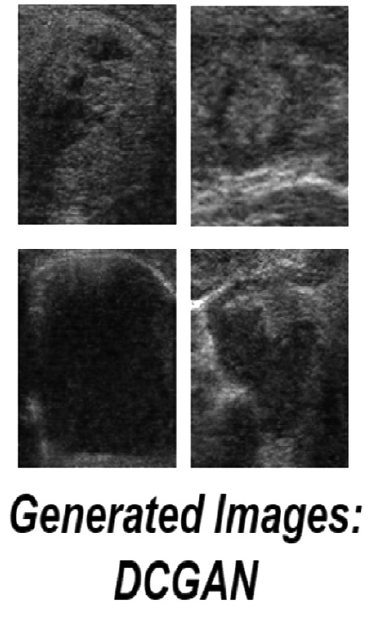
\includegraphics[width=0.35\textwidth]{2/figures/vitpaper6_part1.png}
		\caption[Imágenes de ultrasonido de la tiroides generadas]{Imágenes de ultrasonido de la tiroides generadas. \\
		Fuente: \cite{pr_JERBI2023autoclassViTGAN}. \textit{Automatic classification of ultrasound thyroids images using vision transformers and generative adversarial networks}.}
		\label{2:fig122}
	\end{center}
\end{figure}

La arquitectura del modelo generador consta de una entrada que es ruido generado aleatoriamente a través de una distribución normal estándar, luego se pasa a través de seis convoluciones 2D transpuestas (fractionally-strided convolution) con tamaño de kernel 4 x 4 con el fin de hacer up-sampling hasta llegar al tamaño de 128 x 128. Todas las capas convolucionales excepto la primera tienen un stride de 2. La primera tiene el stride definido en 1 pixel. Finalmente, se usa ReLU en todas las capas convolucionales a excepción del a última. 

La parte de la arquitectura encargada de discriminar tiene una entrada de tamaño 3 x 128 x 128. Este parte del modelo también incluye 6 capas de convolución 2D con un kernel de 4 x 4 y un stride de 2 para todas la capas a excepción de la capa final. Se usó Leaky ReLU con pendiente negativa de 0.2 como función de activación en todas la capas sin contar la capa final que se definió la función sigmoide.

Para la división del conjunto de datos, se usaron dos métodos distintos. El primero consistía en dividir el toda la data en 80\% para el entrenamiento (4 000 imágenes de nódulos benignos y 4 000 imágenes de nódulos malignos), 10\% (500 benignos y 500 malignos) para la validación y 10\% (500 benignos y 500 malignos) para la prueba. El segundo método fue el cross-validation con k-fold de tamaño de 10; es decir, se tomaron 9 000 imágenes para el entrenamiento y 1 000 para la prueba.

Las Redes Neuronales Convolucionales VGG16, EffecientNetB0 y ResNet50 se probaron con el conjunto de datos (dividido por los dos métodos mencionados) utilizando Transfer Learning. En la parte del clasificador se usó Softmax y SVM con un kernel igual a l2. Esta parte sirvió para definir cuál modelo CNN será usado para la implementación de la arquitectura híbrida.

La arquitectura de ViT usada fue el ViTB16. Este modelo recibe patches de 16 x 16. Es decir, las imágenes de ultrasonido se dividirán, de acuerdo a su tamaño, en patches de tamaño 16 x 16. Luego, cada uno de estos es aplanado y mapeado a través de una proyección lineal.

A la secuencia de embedded patches se le añade un nuevo tipo de embedding a la posición 0. Además, se añade otros embeddings 1D a cada embedded patch que indiquen sus respectivas posiciones. Esto finalmente será usado en el encoder del transformer.

El Transformer Encoder consta de un Multi-Head Self Attention (MSA) y un Perceptrón Multicapa (MLP) (dos capas con función GELU), donde la salida del MSA es alimentada al MLP.

La investigación propone que en lugar de alimentar con patches al modelo transformer, se use las salidas de un modelo CNN (ResNet50) como entrada. Esto se logra a través de pasar por un proceso de patching a los tensores resultantes del modelo CNN.

Los modelos CNN y ViT fueron entrenados con los mismos hiper-parámetros (optimizador SGD, tasa de aprendizaje de 0.0001, tamaño de lote de 32, 20 épocas e imágenes de 128 x 128).

En el caso específico de los modelos ViT se usó la función de activación Softmax con la función de pérdida Binary-Cross Entropy. En el caso del clasificador SVM, se usó el kernel l2, función de activación lineal y función de pérdida hinge.

Las métricas usadas para evaluar los modelos entrenados fueron el Accuracy, Precision, Recall y F1-score.

Los resultados se muestran en la Tabla \ref{2:table28}.

\begin{table}[H]
	\caption[Comparación de los modelos entrenados]{Comparación de los modelos entrenados.}
	\label{2:table28}
	\centering
	\small
	\begin{tabular}{ccccccc}
		\specialrule{.1em}{.05em}{.05em}
		{} & {Modelo} & {División de datos} & {F1-score} & {Recall} & {Precision} & {Accuracy} \\
		\specialrule{.1em}{.05em}{.05em}
		\multirow{10}{4cm}{Softmax Classifier} & {VGG16} & {División clásica} & {93.06\%} & {93.06\%} & {93.06\%} & {92.90\%} \\
		{} & {EffecientNetB0} & {División clásica} & {86.42\%} & {86.42\%} & {86.42\%} & {86.40\%} \\
		{} & {RestNet50} & {División clásica} & {96.67\%} & {96.67\%} & {96.67\%} & {96.60\%} \\
		{} & {ViT-B16} & {División clásica} & {92.28\%} & {92.28\%} & {92.28\%} & {92.10\%} \\
		{} & {Hybrid ViT} & {División clásica} & {97.87\%} & {97.87\%} & {97.87\%} & {97.50\%} \\

		{} & {VGG16} & {10-Folds} & {93.24\%} & {93.24\%} & {93.24\%} & {93.42\%} \\
		{} & {EffecientNetB0} & {10-Folds} & {87.09\%} & {87.09\%} & {87.09\%} & {87.16\%} \\
		{} & {RestNet50} & {10-Folds} & {96.66\%} & {96.66\%} & {96.66\%} & {96.71\%} \\
		{} & {ViT-B16} & {10-Folds} & {96.10\%} & {96.10\%} & {96.10\%} & {95.98\%} \\
		{} & {Hybrid ViT} & {10-Folds} & {96.96\%} & {96.96\%} & {96.96\%} & {97.10\%} \\

		\multirow{10}{4cm}{SVM Classifier} & {VGG16} & {División clásica} & {92.78\%} & {90.82\%} & {94.96\%} & {93.69\%} \\
		{} & {EffecientNetB0} & {División clásica} & {85.38\%} & {76.85\%} & {96.42\%} & {90.79\%} \\
		{} & {RestNet50} & {División clásica} & {95.98\%} & {94.14\%} & {98.03\%} & {97.20} \\
		{} & {ViT-B16} & {División clásica} & {94.55\%} & {92.08\%} & {97.23\%} & {95.09\%} \\
		{} & {Hybrid ViT} & {División clásica} & {96.42\%} & {94.82\%} & {98.24\%} & {96.80\%} \\

		{} & {VGG16} & {10-Folds} & {92.29\%} & {90.86\%} & {93.98\%} & {93.44\%} \\
		{} & {EffecientNetB0} & {10-Folds} & {83.95\%} & {75.38\%} & {95.46\%} & {90.51\%} \\
		{} & {RestNet50} & {10-Folds} & {96.46\%} & {94.96\%} & {98.16\%} & {97.32\%} \\
		{} & {ViT-B16} & {10-Folds} & {96.12\%} & {95.14\%} & {97.18\%} & {96.17\%} \\
		{} & {Hybrid ViT} & {10-Folds} & {96.67\%} & {95.01\%} & {98.51\%} & {97.63\%} \\

		\specialrule{.1em}{.05em}{.05em}
	\end{tabular}
	\begin{flushleft}	
		\small Fuente: \cite{pr_JERBI2023autoclassViTGAN}. \textit{Automatic classification of ultrasound thyroids images using vision transformers and generative adversarial networks}.
	\end{flushleft}
\end{table}

En relación a los modelos CNN, se pudo observar que el de mayor desempeño fue el RestNet50 con el clasificador SVM, alcanzando un accuracy de 97.32\%. Este hallazgo permitió determinar el CNN a usar en el modelo híbrido propuesto (ResNet50-ViTB16) que obtuvo finalmente el mejor desempeño general con un accuracy de 97.63\%.

Según \cite{pr_gong2022ACL} encontrar un nódulo tiroideo es relativamente común en varios casos clínicos, pues tiene una tasa de incidencia del 19\% al 68\%, de los cuales un 5\% al 15\% son malignos. Además, existe una gran variedad de imágenes médicas que puede pueden ser usadas para su diagnóstico, siendo las imágenes de ultrasonido la de mayor uso al momento de diagnósticas si un nódulo tiroideo es benigno o maligno. Sin embargo, este tipo de imágenes tiene un gran problema, es que no existe un estándar definido para tomar este tipo de imágenes a diferencia de otros tipos de imágenes como lo son las imágenes tomográficas. Esto conlleva a que las imágenes de ultrasonido sean muy variantes, de distintas resoluciones y con diferentes niveles de ruido. Es por todo esto que se menciona la alta necesidad de desarrollar un siste CAD capaz de aumentar la precisión en el proceso de diagóstico de nódulo tiroideos.

Para el desarrollo de este tipo de sistema, en la investigación se propuso el uso de un nuevo marco de trabajo denominado Adaptative Curriculum Learning (ACL), utilizado en el proceso de entrenamiento y que es capaz de abordar el problema de etiquetas inconsistentes presente en la tarea de clasificación de nódulos tiroideos.

El framework ACL tiene la capacidad de forzar al modelo entrenado a enfocarse en primera instancia en las imágenes más fácilas de clasificar y, posteriormente, en las más difíciles de forma gradual. Aquellas imágenes con etiquetas inconsistentes son descartadas del proceso de entrenamiento otorgándoles una pérdida de cero.

En el proceso de entrenamiento, con cada mini lote de imágenes, el modelo realiza predicciones y el nivel de confianza sobre cada una de las muestras. Luego, en la cola de muestras difíciles, se añaden aquellas muestras que el modelo clasificó de forma incorrecta, mientras que en la cola de certeza, se añaden las confianzas máximas calculadas de cada predicción realizada en el lote. Ya con estas dos colas pobladas, se procede a calcular el umbral adaptativo (T-ada) a través de ambas colas. Este umbral es usado para determinar la forma de cálculo de las pérdidas: si la confianza de predicción es superior al umbral, se calcula la pérdida a través de la entropía cruzada, en caso contrario, la muestra es descartada y se le asigna una pérdida de cero. Finalmente, la pérdida total del lote es calculada a través de la suma de todas las pérdidas de aquellas muestras que no han sido descartadas. Esta pérdida total calculada es usada para el proceso de retropropagación del modelo.

Todo este proceso de entrenamiento con el ACL se puede observar en la Figura \ref{2:fig123}.

\begin{figure}[H]
	\begin{center}
		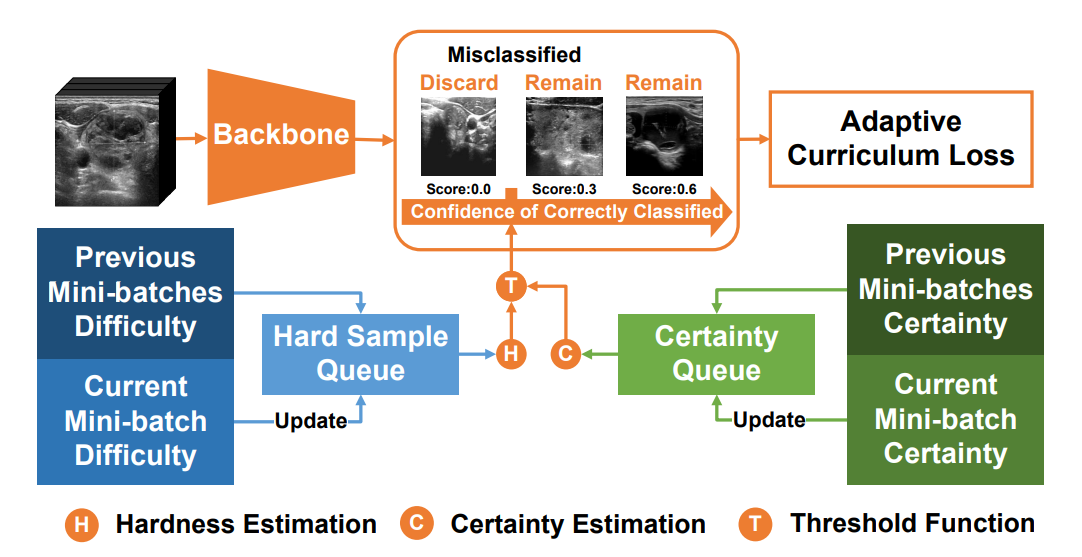
\includegraphics[width=0.80\textwidth]{2/figures/acl_process.png}
		\caption[Proceso de entrenamiento con ACL]{Proceso de entrenamiento con ACL. \\
		Fuente: \cite{pr_gong2022ACL}. \textit{Less is More: Adaptive Curriculum Learning for Thyroid Nodule Diagnosis}.}
		\label{2:fig123}
	\end{center}
\end{figure}

Para realizar el entrenamiento de sus modelos con ACL, en la investigación se propone el uso del conjunto de datos TNCD (Thyroid Nodule Classification Dataset) que consiste de 3 493 imágenes de ultrasonido de nódulos tiroideos de 2 421 pacientes, y dividido en subconjuntos de entrenamiento y prueba, con el primero que consta de 2 879 imágenes (1 905 benignos y 974 malignos) y el segundo de 614 imágenes (378 benignos y 236 malignos). Este conjunto de datos es otorgado por el mismo repositorio online y de acceso libre de los investigadores, con el fin de facilitar futuras investigaciones en el área.

Los backbone utilizados para el proceso de entrenamiento junto con el ACL fueron las arquitecturas de ResNet18, DenseNet121 y ConvNeXt-Tiny. Estos modelos fueron comparados con otras funciones de pérdida basadas en el aprendizaje curricular avanzado (Curriculum Loss y SuperLoss) y aplicadas con los mismos backbone.

Todos los modelos fueron entrenados con el NVIDIA 3090 GPU y Pytorch. Los pesos iniciales fueron fueron sacados de las arquitecturas preentrenadas con ImageNet. El optimizador fue el Stochastic Gradient Descent (SGD) y una tasa de aprendizaje de 0.001. Las imágenes fueron redimensionadas a 224 x 224 píxeles, y se aplicó un aumento a través de un giro horizontal. Este proceso de Aumento de datos se aplicó a la clase minoritaria (imágenes de nódulos benignos). Finalmente, se definió a 16 el tamaño de lote y cantidad de épocas.

Los resultados del entrenamiento se presentan en la Tabla \ref{2:table29}.

\begin{table}[H]
	\caption[Resultados del entrenamiento de los modelos con ACL]{Resultados del entrenamiento de los modelos con ACL.}
	\label{2:table29}
	\centering
	\small
	\begin{tabular}{p{2.8cm}cccccc}
		\specialrule{.1em}{.05em}{.05em}
		{Est. de Aprendizaje} & {Backbone} & {Accuracy} & {Precision} & {Recall} & {F1-score} & {AUC} \\
		\specialrule{.1em}{.05em}{.05em}
		\multirow{3}{4cm}{Cross Entropy} & {ResNet18} & {70.75\%} & {61.71\%} & {68.05\%} & {64.47\%} & {77.31\%} \\
		{} & {DenseNet121} & {70.36\%} & {63.92\%} & {63.31\%} & {63.31\%} & {78.05\%} \\
		{} & {ConvNeXt-Tiny} & {72.29\%} & {62.94\%} & {71.19\%} & {66.36\%} & {78.38\%} \\
		\hline
		\multirow{3}{4cm}{CL} & {ResNet18} & {70.54\%} & {62.87\%} & {65.85\%} & {64.04\%} & {76.98\%} \\
		{} & {DenseNet121} & {70.03\%} & {62.44\%} & {65.25\%} & {63.31\%} & {77.27\%} \\
		{} & {ConvNeXt-Tiny} & {72.14\%} & {60.21\%} & {75.76\%} & {67.00\%} & {74.37\%} \\
		\hline
		\multirow{3}{4cm}{SL} & {ResNet18} & {71.26\%} & {64.97\%} & {64.15\%} & {64.46\%} & {78.50\%} \\
		{} & {DenseNet121} & {71.82\%} & {64.38\%} & {66.86\%} & {65.42\%} & {78.98\%} \\
		{} & {ConvNeXt-Tiny} & {71.47\%} & {62.66\%} & {68.39\%} & {65.36\%} & {77.87\%} \\
		\hline
		\multirow{3}{4cm}{ACL} & {ResNet18} & {73.28\%} & {63.02\%} & {73.64\%} & {67.87\%} & {79.89\%} \\
		{} & {DenseNet121} & {72.92\%} & {60.74\%} & {77.80\%} & {67.99\%} & {79.84\%} \\
		{} & {ConvNeXt-Tiny} & {72.50\%} & {61.19\%} & {74.75\%} & {67.21\%} & {78.85\%} \\
		\specialrule{.1em}{.05em}{.05em}
	\end{tabular}
	\begin{flushleft}	
		\small Fuente: \cite{pr_gong2022ACL}. \textit{Less is More: Adaptive Curriculum Learning for Thyroid Nodule Diagnosis}.
	\end{flushleft}
\end{table}

Los resultados muestran la superioridad de la estrategia de aprendizaje con ACL en comparación con las otras estrategias de aprendizaje, superando en las métricas de Accuracy, F1-score y AUC a los demás modelos.

\end{comment}

\cite{bicbic2023automated} En este estudio, Jasmin Bicbic, Thomas Emmanuel Gabriel Macatangay y su equipo desarrollaron un sistema de detección automática de daños en pavimentos para Filipinas, empleando el modelo YOLOv5n6 junto con un dispositivo Jetson Nano. Este enfoque permite la detección en tiempo real de daños como grietas, fisuras de cocodrilo y baches, eliminando la necesidad de inspecciones manuales en carreteras de alto tráfico y condiciones ambientales variables.

La selección del modelo YOLOv5n6 responde a su capacidad para equilibrar precisión y velocidad en el procesamiento, mientras que Jetson Nano permite una implementación eficiente de YOLOv5n6, proporcionando un sistema ágil y adaptable. Durante las pruebas, el modelo alcanzó una precisión superior al 90\% en la clasificación de daños, mostrando una notable robustez ante variaciones en la luz y el clima. La adaptabilidad del sistema, unida a su precisión en clasificación, representa un avance considerable para países con redes viales extensas y recursos limitados.

Resultados y Rendimiento: El modelo YOLOv5n6 en Jetson Nano demostró altas tasas de precisión, superando el 90\% en pruebas controladas de campo. Su capacidad de análisis en tiempo real permite identificar y clasificar rápidamente daños en el pavimento, facilitando la priorización de mantenimiento.

Conclusiones y Futuras Aplicaciones: Este sistema contribuye significativamente a la eficiencia en el mantenimiento vial, minimizando costos y mejorando la seguridad. Los autores proponen mejoras futuras para maximizar la precisión y extender su uso a otros tipos de pavimento y áreas rurales, anticipando su utilidad para un mantenimiento preventivo de alcance nacional.
\cite{ren2024annotated} Este trabajo, liderado por Miao Ren y su equipo, desarrolla un recurso robusto para la detección automática de daños en pavimentos llamado SVRDD (Street View Road Damage Dataset), un conjunto de datos de imágenes de calle en Beijing. SVRDD fue creado para mejorar el rendimiento de modelos de detección de objetos mediante el entrenamiento en datos reales de grietas longitudinales, transversales, fisuras de cocodrilo y baches. Utilizando imágenes georreferenciadas y anotadas de Baidu Maps, SVRDD abarca más de 20,000 instancias de daños, proporcionando una base sólida para el desarrollo de algoritmos precisos.

Al evaluar el conjunto SVRDD, se utilizaron modelos de detección de objetos como YOLOv5, YOLOX y Cascade R-CNN. YOLOv5 se destacó en términos de velocidad y precisión, alcanzando una precisión promedio (mAP@0.5) de 0.733 y un F1-Score de 0.709, lo que lo convierte en una elección óptima para la clasificación de daños en múltiples condiciones ambientales.

Resultados y Rendimiento: El rendimiento de YOLOv5 en el conjunto de datos SVRDD superó las expectativas en términos de precisión y eficiencia, destacando su potencial en la identificación de diferentes tipos de daños de pavimento en entornos variados.

Conclusiones y Futuras Aplicaciones: El SVRDD facilita avances en la visión por computadora aplicada al mantenimiento vial. La disponibilidad pública del dataset fomenta investigaciones futuras en diversas áreas urbanas y climas, ampliando la aplicabilidad de modelos de detección en imágenes de vista callejera y promoviendo la gestión eficiente de infraestructuras viales.

\cite{crackseverity2023dl} La investigación realizada por este equipo se centra en el uso de segmentación basada en aprendizaje profundo para evaluar la severidad de grietas en pavimentos, utilizando modelos de segmentación que combinan redes neuronales convolucionales (CNN) con técnicas avanzadas de detección. El enfoque está diseñado para detectar y clasificar daños de pavimento en diferentes categorías de severidad, proporcionando una evaluación detallada y precisa.

El estudio evaluó varios modelos de segmentación en diferentes condiciones de luz y resolución, y la implementación de CNN mostró ser particularmente eficaz para identificar grietas, baches y otros tipos de daños, alcanzando niveles de precisión superiores al 90\% en la segmentación de daños severos y leves. Este modelo demostró ser capaz de clasificar eficientemente grietas en tiempo real, facilitando la priorización de las reparaciones de acuerdo con la severidad.

Resultados y Rendimiento: Las pruebas controladas mostraron que el modelo CNN podía clasificar y segmentar daños con una precisión superior al 90\%, adaptándose a diversas condiciones y resoluciones de imagen, lo que facilita su implementación en sistemas de monitoreo vial.

Conclusiones y Futuras Aplicaciones: Este enfoque de segmentación profunda permite una evaluación proactiva de los daños en pavimentos, optimizando el mantenimiento al categorizar la severidad de los daños. Los autores planean integrar más datos y mejorar la precisión para implementar esta solución en redes viales más amplias, aportando a la conservación preventiva de infraestructura vial en diversas condiciones urbanas y rurales.


\cite{romangaray2023segformer} La investigación de Mario Alberto Roman-Garay, Luis Alberto Morales-Rosales, Héctor Rodríguez-Rangel y Sofía Isabel Fernández-Gregorio se centra en un enfoque automatizado para la detección de deterioros superficiales en pavimentos, empleando redes neuronales avanzadas de tipo Transformer. La necesidad de identificar de manera temprana y precisa grietas y baches en pavimentos flexibles es crítica para la seguridad vial y la eficiencia en el mantenimiento, permitiendo acciones preventivas que pueden reducir costos y evitar deterioros graves en infraestructuras clave. El modelo utilizado, llamado Segformer, aborda el problema mediante segmentación semántica, adaptándose a condiciones ambientales diversas gracias a la robustez de esta arquitectura de red.

Para entrenar el modelo, los autores crearon un conjunto de datos inicial de 245 imágenes tomadas en diversas calles de Culiacán, México, bajo diferentes condiciones de iluminación y presencia de sombras. Con el fin de mejorar el rendimiento y la precisión del modelo, el conjunto se expandió mediante técnicas de aumento de datos, como el contraste y la rotación, alcanzando un total de 2052 imágenes. Estas imágenes fueron etiquetadas y preprocesadas, utilizando una cámara GoPro 8 Black a una altura de 1.20 metros para capturar de manera óptima la superficie de los pavimentos.

Modelo y Metodología: La arquitectura Segformer está diseñada específicamente para tareas de segmentación y detección en entornos no controlados. Utiliza un codificador que extrae características gruesas y finas de las imágenes, seguido de un decodificador que combina estas características para generar una máscara de segmentación precisa. Esto permite al modelo identificar de forma confiable daños específicos, como grietas y baches, independientemente de variaciones en las condiciones de luz o sombras. Además, se implementaron técnicas de preprocesamiento de imágenes, como el estiramiento de contraste y la conversión a escala de grises, con el objetivo de resaltar detalles críticos en las imágenes y reducir el impacto de elementos externos que pudieran interferir en el análisis.

Resultados y Rendimiento: Los resultados del modelo Segformer fueron evaluados en términos de precisión, recall y F1 Score, alcanzando métricas significativas: una precisión del 82.35\%, un F1 Score de 88.89\% y un recall de 96.55\%. Esto indica que el modelo logró detectar correctamente la mayoría de los daños superficiales en pavimentos, con un mínimo de falsos positivos, superando a otros métodos de procesamiento de imágenes y redes convolucionales en situaciones similares. El modelo mostró una alta efectividad al identificar grietas y baches incluso en condiciones desafiantes, lo que demuestra su robustez en entornos reales.

Conclusiones y Futuras Aplicaciones: Esta investigación contribuye con una metodología eficaz y aplicable para la conservación de infraestructuras viales, donde el uso de redes Transformer permite un análisis de alta precisión en diferentes tipos de pavimentos y condiciones ambientales. La implementación de este modelo en el ámbito de la gestión vial podría facilitar una monitorización continua y detallada del estado de los pavimentos, optimizando la planificación de reparaciones y asignación de recursos. Los autores sugieren ampliar el conjunto de datos y explorar mejoras en el modelo para incluir medidas de severidad en el análisis, como la longitud, anchura y profundidad de las grietas, para una evaluación más exhaustiva de los daños y su impacto en la infraestructura vial.

\begin{comment}
faltan citas en bibtex	

Goodfellow, I., Bengio, Y., & Courville, A. (2016). Deep Learning. MIT Press.
Redmon, J., Divvala, S., Girshick, R., & Farhadi, A. (2016). You Only Look Once: Unified, Real-Time Object Detection. In Proceedings of the IEEE Conference on Computer Vision and Pattern Recognition (CVPR).
Carion, N., Massa, F., Synnaeve, G., et al. (2020). End-to-End Object Detection with Transformers. European Conference on Computer Vision (ECCV).
\end{comment}

\section{Bases Teóricas}
\subsection{Deep Learning}

El Deep Learning o Aprendizaje Profundo es una rama del Machine Learning que conforma varios tipos de algoritmos y enfoques mucho más amplios. Este involucra tratar a los problemas que requiere mayor generalización como lo es la visión por computadora y el reconocimiento de voz. Es decir, estos problemas generales se refieren a problemas que los humanos pueden resolver con facilidad. El Deep Learning involucra al Aprendizaje Supervisado, No Supervisado y el Aprendizaje por Refuerzo. El concepto de “profundidad” se refiere a la característica de sus enfoques en usar muchas capas de redes neuronales artificiales, donde cada una de estas realiza una operación especial, para que en conjunto su complejidad y potencia de resolución de problemas sea mayor. \parencite{bk_hurbans2020grokking}


El aprendizaje profundo (Deep Learning) ha revolucionado el campo de la inteligencia artificial y, en particular, el de la visión por computadora. Se basa en el uso de redes neuronales artificiales con múltiples capas, que permiten aprender representaciones jerárquicas de datos. Este enfoque ha demostrado ser particularmente efectivo en tareas de clasificación y detección de objetos debido a su capacidad para procesar grandes volúmenes de datos y extraer características complejas de imágenes.


El aprendizaje profundo se inspira en la estructura y funcionamiento del cerebro humano, donde las neuronas procesan información y transmiten señales. Las redes neuronales profundas (DNNs, por sus siglas en inglés) se componen de capas de neuronas, donde cada capa transforma la entrada en una representación más abstracta. Por ejemplo, en una red convolucional, las capas iniciales pueden detectar bordes y texturas, mientras que las capas más profundas pueden reconocer formas y objetos completos.

Un modelo popular en el campo de la detección de objetos es la red neuronal convolucional (CNN), que utiliza operaciones de convolución para extraer características espaciales de las imágenes. Según Goodfellow, Bengio y Courville (2016), "las redes neuronales convolucionales han sido utilizadas exitosamente para el reconocimiento de imágenes, superando a otros enfoques anteriores en términos de precisión y eficiencia" (Goodfellow et al., 2016).

En la detección de objetos, los modelos de aprendizaje profundo han permitido avances significativos. Por ejemplo, la arquitectura YOLO (You Only Look Once) es un modelo de detección en tiempo real que divide la imagen en una cuadrícula y predice las cajas delimitadoras y las clases de los objetos simultáneamente. Este enfoque ha demostrado ser rápido y preciso, lo que lo hace ideal para aplicaciones en tiempo real.

Un estudio de Redmon et al. (2016) sobre YOLO destaca que "la capacidad de YOLO para procesar imágenes en tiempo real sin sacrificar la precisión lo convierte en una herramienta valiosa para tareas de detección de objetos en diversas aplicaciones, desde vehículos autónomos hasta monitoreo de infraestructuras" (Redmon et al., 2016).

Con el auge de arquitecturas más avanzadas, como las redes Transformer, el aprendizaje profundo ha continuado evolucionando. Modelos como DETR (DEtection TRansformer) han mostrado un enfoque novedoso al tratar la detección de objetos como un problema de secuencia a secuencia, mejorando la precisión en tareas complejas de detección y localización.

Investigaciones recientes han demostrado que las arquitecturas basadas en Transformers, combinadas con técnicas de aprendizaje profundo, ofrecen mejoras en la precisión y capacidad de generalización en comparación con las redes convolucionales tradicionales. Según Carion et al. (2020), "DETR logra una alta precisión en la detección de objetos al abordar el problema como una tarea de atención, permitiendo una mejor captura de relaciones espaciales en las imágenes" (Carion et al., 2020).

El aprendizaje profundo ha transformado la manera en que se aborda la detección de objetos, proporcionando herramientas poderosas para la automatización y el análisis en diversos dominios. La continua evolución de las arquitecturas de redes neuronales promete aún más avances en la precisión y eficiencia de estas tecnologías, lo que es fundamental para aplicaciones críticas como el mantenimiento de infraestructuras viales y la seguridad pública.
\begin{comment}
	

\begin{figure}[H]
	\begin{center}
		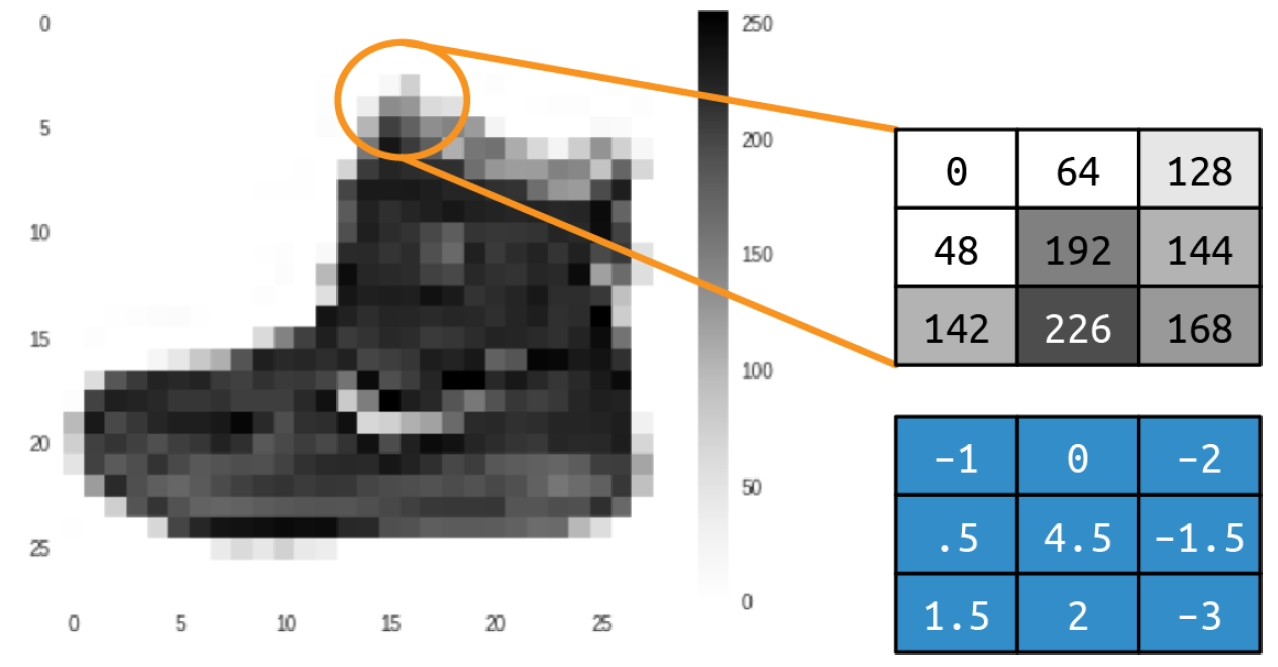
\includegraphics[width=0.80\textwidth]{2/figures/cnn_fash_mnist.png}
		\caption[Convolución de imagen de Fashion MNIST]{Convolución de imagen de Fashion MNIST. \\
		Fuente: \cite{bk_moroney2020aiandml}. \textit{AI and Machine Learning for Coders}.}
		\label{2:fig201}
	\end{center}
\end{figure}

Con un filtro de 3x3 como se muestra en la imagen, se puede modificar el valor del pixel. Este proceso se repite con cada pixel en imagen. Finalmente, se obtiene una imagen nueva conocida como una imagen filtrada. \parencite{bk_moroney2020aiandml} En el ejemplo anterior, el nuevo valor del pixel original 192 será 577, pues este es el resultado de multiplicar, y posteriormente sumar, los pesos del filtro con el valor del pixel y sus vecinos.

Existen distintos tipos de filtros que modifican y otorgan distintos tipos de resultados. Como ejemplo se presenta la Figura \ref{2:fig202} y la Figura \ref{2:fig203}.

\begin{figure}[H]
	\begin{center}
		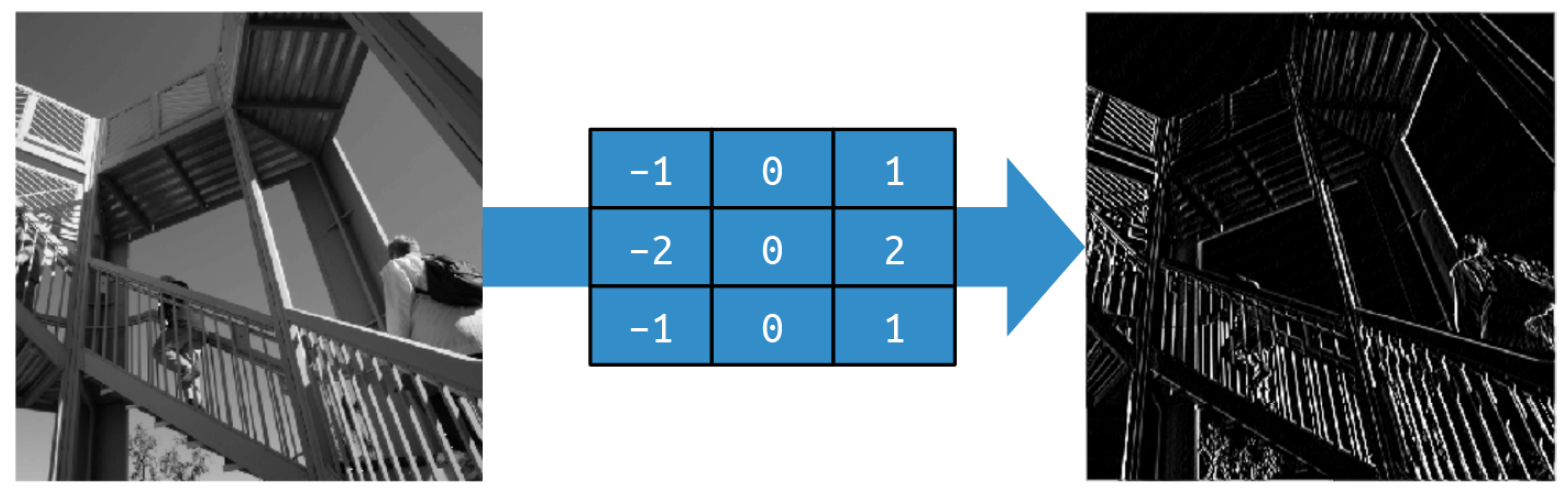
\includegraphics[width=1.00\textwidth]{2/figures/cnn_filtro_vert.png}
		\caption[Convolución de imagen con filtro de líneas verticales]{Convolución de imagen con filtro de líneas verticales. \\
		Fuente: \cite{bk_moroney2020aiandml}. \textit{AI and Machine Learning for Coders}.}
		\label{2:fig202}
	\end{center}
\end{figure}

\begin{figure}[H]
	\begin{center}
		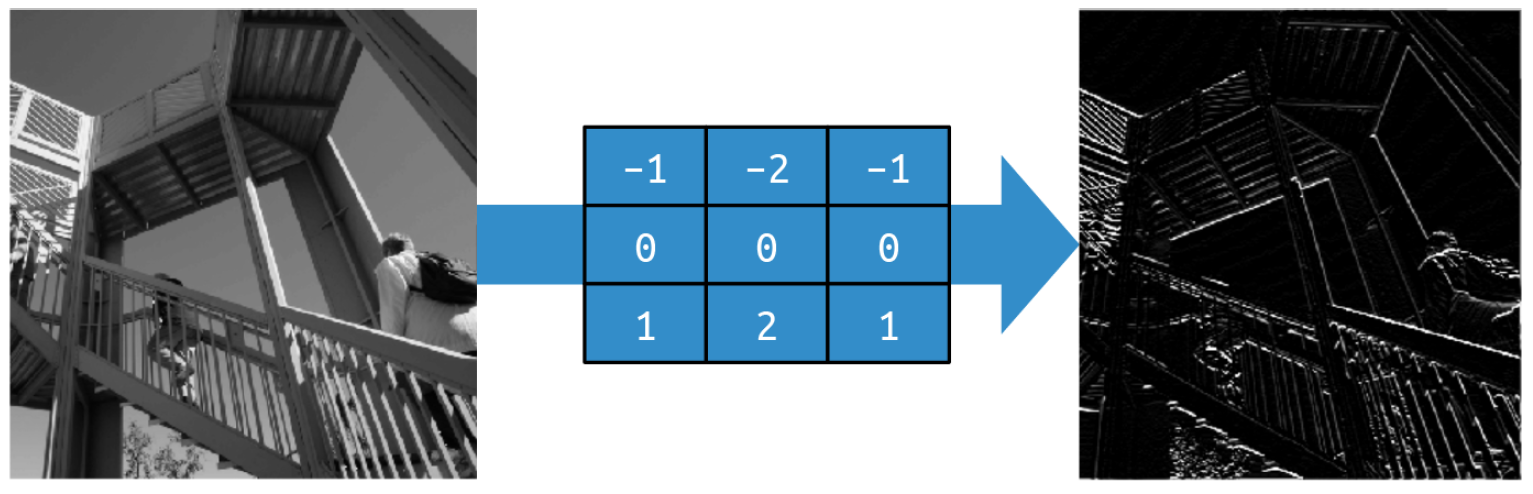
\includegraphics[width=1.00\textwidth]{2/figures/cnn_filtro_hori.png}
		\caption[Convolución de imagen con filtro de líneas horizontales]{Convolución de imagen con filtro de líneas horizontales. \\
		Fuente: \cite{bk_moroney2020aiandml}. \textit{AI and Machine Learning for Coders}.}
		\label{2:fig203}
	\end{center}
\end{figure}

El primer filtro realiza modificaciones a una imagen original para finalmente obtener otra imagen distinta en donde se resaltan las líneas verticales. Caso contrario pasa con el segundo filtro, donde la imagen original es modificada para resaltar sus líneas horizontales. Así, existen distintos tipos de filtros con distintos pesos. Cada uno de estos permite resaltar en las imágenes, a través de modificaciones en sus pixeles, sus características más importantes que serán de utilidad para diferenciar entre una clase u otra de un conjunto de imágenes. También se podría decir que esta técnica de aplicar convoluciones permite reducir la cantidad de información presente en las imágenes, entonces se podría aprender o encontrar un conjunto de filtros específicos capaces de reducir la gran cantidad de información de las imágenes en características que estén relacionadas a sus respectivas etiquetas \parencite{bk_moroney2020aiandml}.

Para reducir la cantidad de información presente en las imágenes, manteniendo al mismo tiempo las características obtenidas por las convoluciones, es necesario aplicar otra técnica entro del mundo del Deep Learning.

El proceso de pooling consiste en eliminar cierta cantidad de pixeles en una imagen, mientras se mantienen las partes resaltantes de la misma. Este proceso normalmente se realiza con agrupaciones de 2x2 en los pixeles de una imagen. Estas agrupaciones también son conocidos como pool. Dentro de cada uno de estas se selecciona el máximo valor de pixel. El proceso se repite con nuevos grupos de pixeles para finalmente obtener una nueva imagen de tamaño considerablemente reducido. \parencite{bk_moroney2020aiandml} En la Figura \ref{2:fig204} se presenta un ejemplo gráfico.

\begin{figure}[H]
	\begin{center}
		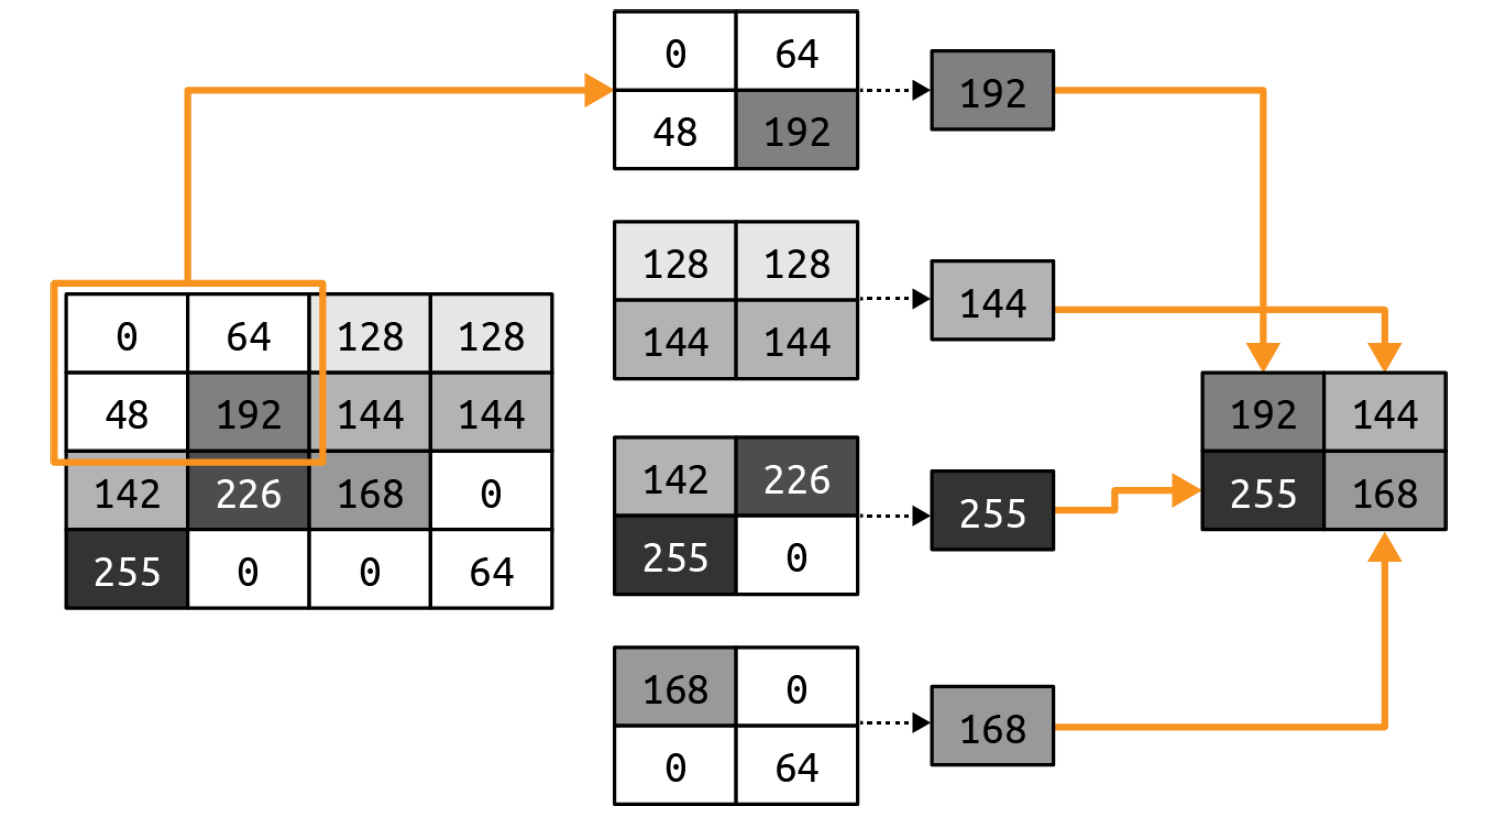
\includegraphics[width=0.85\textwidth]{2/figures/cnn_pool_examp.png}
		\caption[Ejemplo de max-pooling con un pool de 2x2]{Ejemplo de max-pooling con un pool de 2x2. \\
		Fuente: \cite{bk_moroney2020aiandml}. \textit{AI and Machine Learning for Coders}.}
		\label{2:fig204}
	\end{center}
\end{figure}

La imagen original de 4x4 pixeles, luego de ser aplicado el proceso de pooling, se obtiene una imagen reducida de 2x2 pixeles. De manera general, la imagen redujo a la cuarta parte de la cantidad original de pixeles.

Con estas dos técnicas del Deep Learning se han ido desarrollando distintas arquitecturas de redes neurales en la última década. Algunas más complejas y con más capas que otras. Cada una de estas han logrado desempeñarse de forma satisfactoria con el conjunto de datos con el que se han entrenado, demostrando el gran potencial de la Redes Neuronales Convolucionales o CNN.

Algunas de las arquitecturas más conocidas y que han sido usadas en gran variedad de investigaciones son los VGG, ResNet, Inception y DenseNet.

La arquitectura VGG o VGGNet es una red neuronal artificial con una profundidad de 16 o 19 capas (dependiendo de la versión que se analice) y usa pequeños filtros de convolución de tamaño 3x3 a través de estas. Este modelo participó en el ImageNet Challenge 2014, donde logró el primer puesto en las tareas de localización y segundo puesto en clasificación. Además, tiene la alta capacidad de generalización en otros conjuntos de datos, es decir, es capaz de obtener buenos resultados con imágenes distintas a las usadas para su entrenamiento. \parencite{pr_simonyan2015vdcn}

Otra arquitectura bastante difundida en el mundo del Deep Learning y las CNN es ResNet. Esta arquitectura nace de la premisa del aumento de la dificultad de entrenar las redes neuronales profundas. Con el objetivo de facilitar este proceso se añade a las ya conocidas CNN el concepto de residual, para obtener redes residuales que sean mucho más fáciles de optimizar y capaces de obtener mejor desempeño a más grande sea la profundidad de la red. El modelo tuvo 152 capas, ocho veces más grande que las arquitecturas VGG, y fue evaluada con el conjunto de datos ImageNet. \parencite{pr_he2016deepres}

Inception es una arquitectura que obtuvo un alto desempeño en las tareas de clasificación y detección en el ImageNet Large-Scale Visual Recognition Challenge 2014 (ILSVRC14). La principal distinción de este modelo es el uso de los recursos informáticos a través de la red. Esto significa que mientras más aumente la complejidad del modelo a través de su profundidad, los recursos computacionales no variarán a gran escala como se esperaría. Esto se logra a través del uso de módulos de Inception en algunas capas de la arquitectura en general. Los distintos módulos se encuentran apilados unos sobre otros y con algunas capas max-pooling. Dentro de esta arquitectura, se tiene a GoogLeNet, que no es más que una versión de Inception de 22 capas (este modelo fue el presentado a ILSVRC14). \parencite{pr_szegedy2015goingdwc}

DenseNet nace con la premisa de que las CNN pueden obtener mejores desempeños si se tienen conexiones cortas entre las capas cerca de la entrada y salida de la red. La propuesta de esta red consiste en establecer una conexión de cada capa con todas las demás capas de la misma red. Esto trae grandes ventajas como la reducción del problema de gradiente de fuga, fomenta la reutilización de características extraídas en previas capas, además de disminuir la cantidad de parámetros. El modelo fue evaluado con los conjuntos de datos CIFAR-10, CIFAR-100, SVHN e ImageNet para la tarea de reconocimiento de objetos. \parencite{pr_huang2016densconn} En la Figura \ref{2:fig205} se muestra una representación de DenseNet con 5 capas.

\begin{figure}[H]
	\begin{center}
		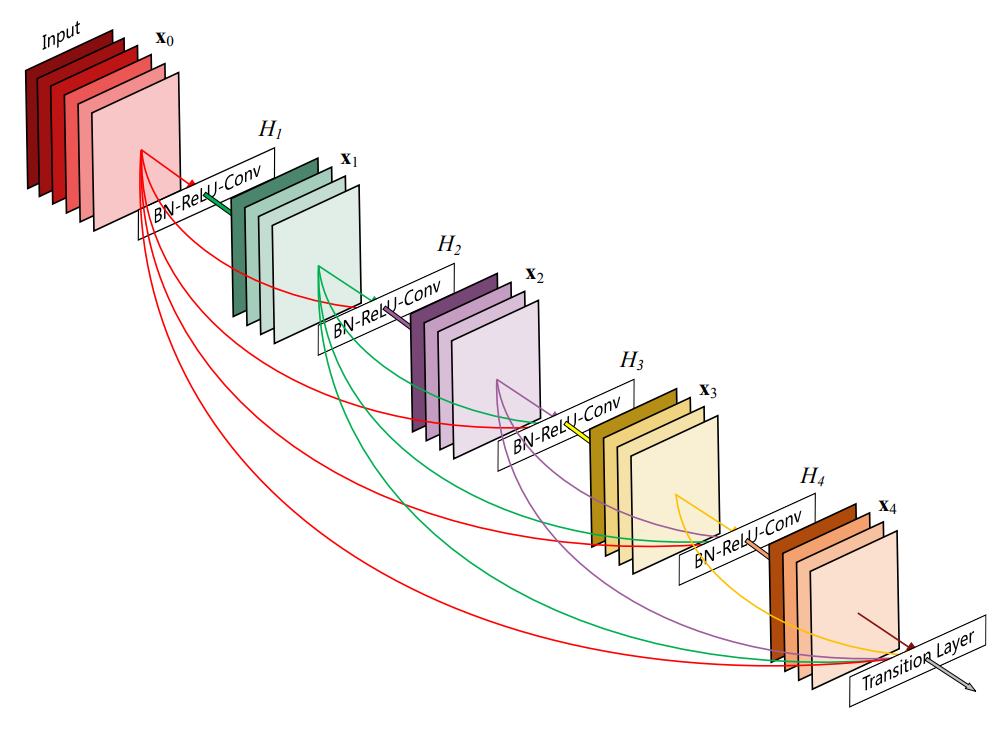
\includegraphics[width=0.70\textwidth]{2/figures/densenet_5lay.png}
		\caption[DenseNet con 5 capas]{DenseNet con 5 capas. \\
		Fuente: \cite{pr_huang2016densconn}. \textit{Densely Connected Convolutional Networks}.}
		\label{2:fig205}
	\end{center}
\end{figure}

% Las tareas relacionadas al procesamiento de imágenes como la segmentación, detección de objetos y clasificación es actualmente dominada por las redes neuronales convolucionales explicadas anteriormente; sin embargo, gracias al gran avance y divulgación de los modelos basados en Transformers, se ha visto el surgimiento de un nueva clase de arquitecturas que prometen mejorar el desempeño de los actuales modelos dominantes: los Vision Transformer (ViT).

A pesar del gran desempeño del los modelos de basados den CNN, los últimos años han aparecido nuevas y prometedoras arquitecturas capaces de superarlos.

Según la investigación original presentada por \cite{pr_dosovitskiy2021animageisworth}, los modelos Transformer, dominantes actuales en tareas de procesamiento de lenguaje natural (NLP), se han convertido en el modelo predilecto cuando se trata de manejo de texto, esto debido a su capacidad de utilizar los recursos computacionales de forma eficiente y su escalabilidad, permitiendo así obtener modelos de; por ejemplo, 100 mil millones de parámetros.

% A diferencia de las tareas de NLP, la visión por computadora tuvo mayores problemas para adaptar este nuevo tipo de arquitecturas a sus tareas específicas.

Según \cite{pr_vaswani2017attentionisallneed} los Transformer tiene una arquitectura similar a los modelos Neural Sequence Transduction que contienen dos partes importantes: encoder y decoder. El encoder se encarga de realizar un mapeo de las entradas a secuencias continuas. El decoder recibe este último para finalmente generar un secuencia de símbolos de forma autorregresiva, generando un símbolo a la vez mientras utiliza los anteriores símbolos ya generados como entrada. El modelo Transformer sigue este mismo comportamiento a través de su mecanismo característico de Self-Attention junto a sus capas conectadas completamente.

En el encoder de las arquitecturas Transformer se tienen 6 capas que se componen de otras 2 subcapas: Multi-Head Self-Attention y Fully Connected Feedforward en función a su posición. Además, entre estas dos subcapas, se aplicaron conexiones residuales y capas de normalización. Finalmente, también se definió una capa de Embedding. La dimensión de los vectores generados por todas estas capas es de 512.

En el decoder también se tienen 6 capas idénticas entre sí. Además, similar al encoder, las dos capas Multi-Head y Fully Connected también están presentes con la diferencia de una nueva subcapa Multi-head que recibe como entrada la salida del encoder. Otra característica distintiva del decoder es el masking aplicado a la capa Multi-Head que surge como medio para evitar que las posiciones tengan la capacidad de atender a las siguientes posiciones. Finalmente, también se emplearon conexiones residuales y capas de normalización de igual manera que en el encoder.

El proceso de Attention en los Transformers se define como el mapeo de vectores de alta dimensionalidad (query, key y value) a una salida (también vector de alta dimensión). Esta salida se calcula mediante a través de pesos, que se obtienen con una función de compatibilidad entre el query y el key, y que son asignados al vector value para finalmente realizar una suma ponderada con estos. Todo este proceso se realiza de forma paralela en sus proyecciones lineales donde sus salidas serán concatenadas y proyectadas nuevamente. A este proceso, se le conoce como Multi-Head Attetion.

Además de las capas de atención, tanto el encoder como decoder del Transformer tienen una subcapa de Fully Connected Feedforward en función a la posición. Este tipo de capa aplica una transformación lineal usando además la función de activación ReLU.

Las capas Embedding son usadas para llevar los token de entradas a vectores de alta dimensionalidad. Mientras que las funciones de transformación lineal y softmax cambian la salida del decoder para obtener las probabilidades predichas.

Junto a los Embedding, y tanto en el encoder y decoder del Transformer, también se definen los Positional Encoding. Estos se encargan de otorgar información sobre la posición de los token en la secuencia a la que pertenecen. Estos tienen la misma dimensión que los propios Embedding.

Cada una de las partes de la arquitectura de los Transformer descritos anteriormente se puede observar de forma gráfica en la Figura \ref{2:fig213}.

\begin{figure}[H]
	\begin{center}
		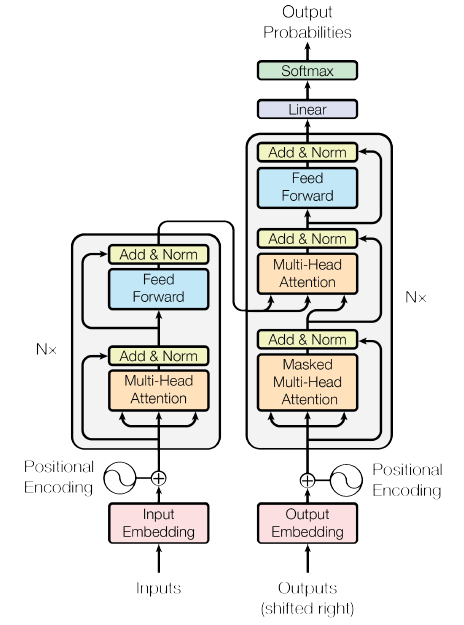
\includegraphics[width=0.70\textwidth]{2/figures/transformer_arch.PNG}
		\caption[Arquitectura del modelo Transformer]{Arquitectura del modelo Transformer. \\
		Fuente: \cite{pr_vaswani2017attentionisallneed}. \textit{Attention is all you need}.}
		\label{2:fig213}
	\end{center}
\end{figure}

En el contexto de la visión por computadora, \cite{pr_dosovitskiy2021animageisworth} menciona que los primeros intentos de uso de esta arquitectura se basaban en aprovechar la capacidad de Self-Attention de los Transformer y combinarlo con los dominantes modelos CNN. Estos intentos de obtener los excelentes resultados de los Transformer en las tareas de visión por computadora no obtenían los resultados de los modelos de mayor desempeño como son los basados en la arquitectura de ResNet.

Debido a esto y al gran potencial que tenían las arquitecturas basadas en Transformers, propusieron el uso de estas arquitecturas aplicadas de forma directa a imágenes; es decir, aplicando la menor cantidad de cambios antes de ingresar al mismo Transformer. El proceso exacto de cómo funciona su arquitectura se explicará más adelante.

La gran ventaja de este nuevo tipo de modelos se basa en la cantidad de datos con la que es entrenado. 

En el caso de usar una pequeña cantidad de imágenes para el entrenamiento se obtienen resultados no favorables, llegando a tener un bajo rendimiento comparado a los modelos basados en CNN. Sin embargo, al realizar su entrenamiento con una mayor cantidad de datos, los Vision Transformer (como se le nombró a este nuevo tipo de arquitectura) obtuvieron mejores resultados que los modelos dominantes en las mismas tareas de visión por computadora.

A diferencia de los Transformer dedica a las tareas de NLP que reciben como entrada token embeddings de una sola dimensión, las imágenes son de dos dimensiones (H, W) y una cantidad de canales (C), lo que dificulta su ingreso directo a este tipo de arquitecturas. Es por esto que es necesario aplicar una división de las imágenes en patches 2D que posteriormente serán aplanados e ingresados al Transformer como haría normalmente los token embeddings.

Estos patches deben tener un tamaño constante P, es decir que se deben obtener divisiones de las imágenes de tamaño P x P. Esto conlleva a que el número de patches final sea igual a $N = HW / P^2$.

Una vez se tienen los N patches, se realiza su aplanamiento y, posteriormente, se mapean en D dimensiones (tamaño del vector latente usado en el Transformer) a través de una proyección lineal capaz de ser entrenada.

Ya obtenidos estos patch embedding, se añade uno nuevo pero con la capacidad de ser aprendible. Estos se agrupan en una secuencia que ingresarán posteriormente al Transforme encoder. Cabe resaltar que, luego de pasar por el encoder, este último embedding añadido representará a la imagen.

A los ya mencionados patch embedding también se le agrega otro tipo de embedding capaz de mantener información relacionada a la posición de cada patch. Estos embedding son 1D y aprendibles. Finalmente, estos serán ingresados juntos con los originales embeddings a Transformer encoder.

En la parte final de la arquitectura se tiene un MLP con la principal tarea de realizar la clasificación de las imágenes. Este MLP consta de una sola capa oculta en la etapa de entrenamiento inicial del modelo, y con una sola capa lineal en la etapa de fine-tuning.

El bloque de Transformer encoder está compuesto por distintos bloques como los multi headed self attention (MSA), MLP y los Layernorm (LN). Estos distintos bloques se van alternando de forma específica, introduciendo además conexiones residuales luego del MSA y MLP.

Toda la arquitectura de los ViT se puede resumir con la Figura \ref{2:fig206}.

\begin{figure}[H]
	\begin{center}
		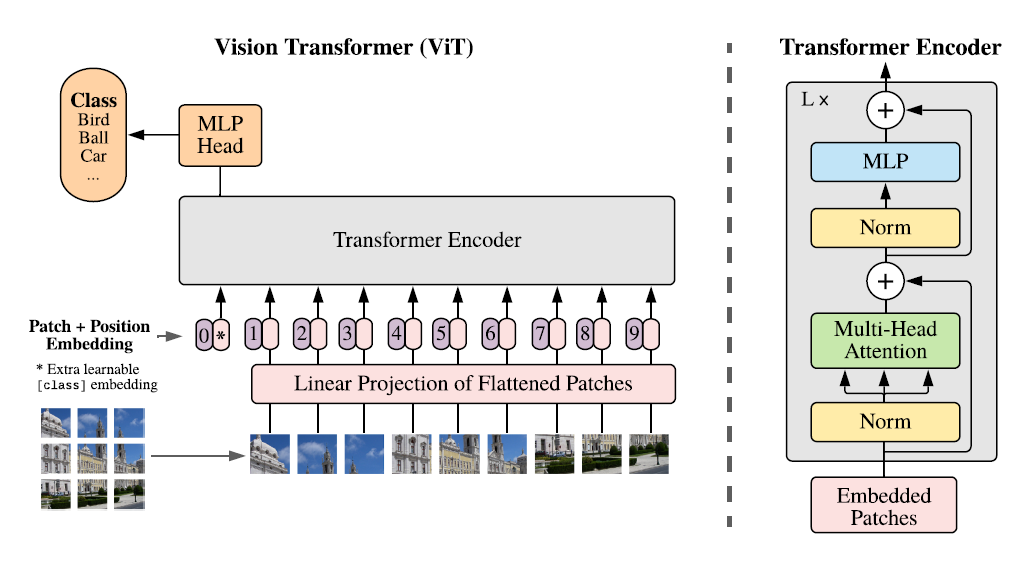
\includegraphics[width=1.00\textwidth]{2/figures/vit_arquitecture.png}
		\caption[Arquitectura del modelo ViT]{Arquitectura del modelo ViT. \\
		Fuente: \cite{pr_dosovitskiy2021animageisworth}. \textit{AN IMAGE IS WORTH 16X16 WORDS: TRANSFORMERS FOR IMAGE RECOGNITION AT SCALE}.}
		\label{2:fig206}
	\end{center}
\end{figure}

\subsection{Transfer Learning}
\cite{bk_geron2022handml} nos menciona que el Transfer Learning o Transferencia de Aprendizaje es un técnica usada en el campo de Deep Learning que permite el uso de algunas capas de un modelo ya definido y entrenado previamente en un nuevo modelo que necesite ser entrenado en una tarea similar al que se desarrolla el modelo original. Las capas destinadas al reuso son normalmente las más cercanas a la entrada o también conocidas como capas inferiores. El beneficio de usar esta técnica radica en dos puntos importantes: cantidad de datos requeridos y velocidad de entrenamiento del modelo; es decir, la cantidad de datos que se deben usar para entrenar un modelo de alto desempeño se reduce considerablemente, mientras que el tiempo requerido para terminar este proceso es menor comparándolo a si lo entrenaran desde cero.

Para que esta técnica funcione debidamente, las capas más cercanas a la salida, conocidas también como capas de alto nivel, deben ser reemplazadas, esto debido a que son más específicas de las tareas del modelo original. Esto también incluye a la capa final, ya que posiblemente no tenga la cantidad de salidas necesarias para completar satisfactoriamente la nueva tarea.

En la Figura \ref{2:fig211} se presenta de forma gráfica la técnica.

\begin{figure}[H]
	\begin{center}
		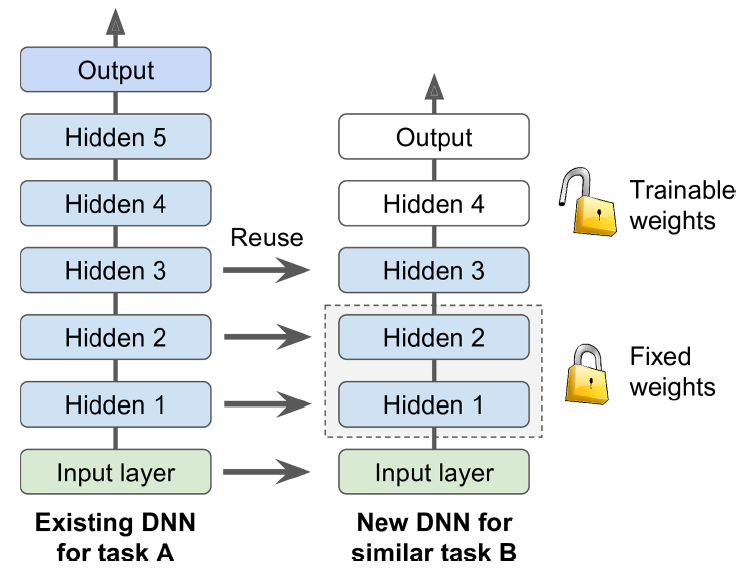
\includegraphics[width=0.70\textwidth]{2/figures/transfer_learning.PNG}
		\caption[Ejemplo de Transfer Learning]{Ejemplo de Transfer Learning. \\
		Fuente: \cite{bk_geron2022handml}. \textit{Hands-on machine learning with Scikit-Learn, Keras, and TensorFlow}.}
		\label{2:fig211}
	\end{center}
\end{figure}

\subsection{Data Augmentation}

Según \cite{bk_geron2022handml} el Aumento de Datos o Data Augmentation es una técnica de regularización que permite reforzar la cantidad de muestras en un conjunto de datos. Esto se realiza a través de la generación de nuevas instancias similares a los originales; es decir, las personas no deberían ser capaces de diferenciar una imagen generada de una del propio conjunto de datos.

Para generar estas nuevas muestras, normalmente se aplican diferentes transformaciones a las instancias del conjunto de datos original. Estas transformaciones pueden ser; por ejemplo, una simple rotación o recorte de la imagen, siempre y cuando no altere por completo su sentido como es el caso de voltear una imagen de texto de forma horizontal. 

El principal beneficio de esta técnica es que permite reducir el sobreajuste de los modelos entrenados. 

En la Figura \ref{2:fig212} se muestran algunas transformaciones que se pueden hacer al aplicar el Aumento de Datos. 

\begin{figure}[H]
	\begin{center}
		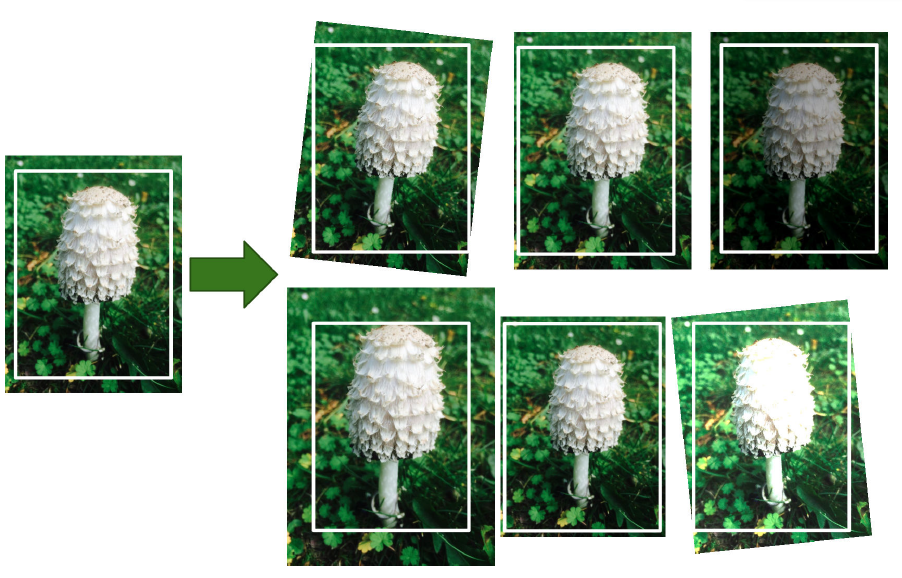
\includegraphics[width=0.85\textwidth]{2/figures/data_aug.PNG}
		\caption[Ejemplo de Data Augmentation]{Ejemplo de Data Augmentation. \\
		Fuente: \cite{bk_geron2022handml}. \textit{Hands-on machine learning with Scikit-Learn, Keras, and TensorFlow}.}
		\label{2:fig212}
	\end{center}
\end{figure}

\subsection{Nódulos Tiroideos}
Para entender qué es un nódulo tiroideo, primero se debe sabes qué es la tiroides. Este es una glándula localizada en el cuello del cuerpo humano que se encarga de producir hormonas que regulan el metabolismo. Los nódulos que aparecen en esta glándula son los más comunes, y se generan debido a un excesivo crecimiento de las células en esa área, estos pueden ser de textura dura o quísticas. \parencite{pr_deng2022autclass}

La Figura \ref{2:fig207} muestra a la glándula en una imagen tomográfica.

\begin{figure}[H]
	\begin{center}
		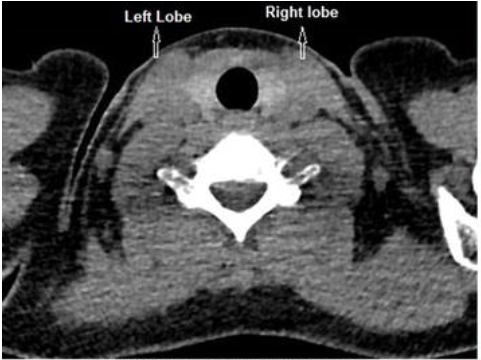
\includegraphics[width=0.55\textwidth]{2/figures/gland_thyroid.png}
		\caption[Imagen tomográfica de glándula de tiroides]{Imagen tomográfica de glándula de tiroides. \\
		Fuente: \cite{pr_binboga2019thyroid}. \textit{Thyroid Anatomy}.}
		\label{2:fig207}
	\end{center}
\end{figure}

\cite{pr_shin2016ultradiag} mencionan que existen algunas características de los nódulos en la tiroides que pueden ser analizados para realizar una clasificación si es de carácter benigno o maligno. A continuación, se presentan aquellos más resaltantes.

El tamaño de nódulos en ciertos casos puede determinar el tipo con el que se está tratando; sin embargo, esto no está debidamente comprobado, a pesar de que normalmente el riesgo de ser maligno de un nódulo es más alto en aquellos de mayor tamaño. Esto principalmente se debe a que los nódulos benignos también pueden llegar a un tamaño considerable, pero con una mayor cantidad de tiempo. Lo que sí puede significar un probable nódulo maligno es un rápido crecimiento de un nódulo sólido.

El contenido interno de un nódulo está determinado por el ratio entre su parte quística y su parte sólida. Los nódulos malignos con contenido sólido poseen mayor riesgo de ser malignos que aquellos con contenido parcialmente quístico.

La ecogenicidad de los nódulos se mide de acuerdo al nivel de brillo en las imágenes de ultrasonido con respecto a otras partes de la imagen. Esto quiere decir que un nódulo es hipoecoico si su nivel de brillo en la imagen es menor con respecto a otra parte de la imagen, específicamente se compara con el músculo anterior del cuello o el parénquima tiroideo. La mayoría de los tumores tiroideos son hipoecoicos, y existe mayor riesgo de que los nódulos con la misma característica sean malignos.

La forma y orientación de los nódulos también pueden determinar si son o no malignos. La manera en que los nódulos malignos crecen es de manera centrífuga y a través del plano del tejido, al igual que los benignos; sin embargo, estos crecen de manera paralela. La forma redonda u ovoide de los nódulos se encuentra en aquellos de carácter benigno; sin embargo, no son propias de este. Una característica mucho más específica de los nódulos de carácter malignos es su orientación no paralela, es decir, son más altos que anchos.

Finalmente, el margen de los nódulos también puede dar información del tipo con el que se trata. Una característica que sugiere que un nódulo es maligno es un margen espiculado o micro tubulado.

\subsection{Ecografía y las imágenes de ultrasonido}
Según \cite{pr_herrera2017diseimp}, la ecografía, que es una técnica de diagnóstico en donde se usan imágenes generadas por ultrasonido, es comúnmente desarrollado en las áreas de cardiología, ginecología, y otras más relacionadas. La popularidad de esta técnica se basa en la capacidad de las imágenes de alta calidad que se obtienen de este proceso, además de no ser un método invasivo o de radiación como muchos otros de su tipo.

Los sistema encargados de extraer las imágenes de ultrasonido son compuestos de distintas sensores que generan ondas de sonido para posteriormente analizar la respuesta de la interacción física con el campo de interés. Estas señales recibidas de regreso son digitalizados por una parte electrónica delantera que también transforman estos datos crudos en la imagen final. El funcionamiento de este proceso depende de la configuración de los sensores, el método usado para obtener las imágenes y las características de área de interés. \parencite{pr_camacho2022ultrasonicimg}

Algunas imágenes de ultrasonido de nódulos tiroideos se muestran en la Figura \ref{2:fig210}.

\begin{figure}[H]
	\begin{center}
		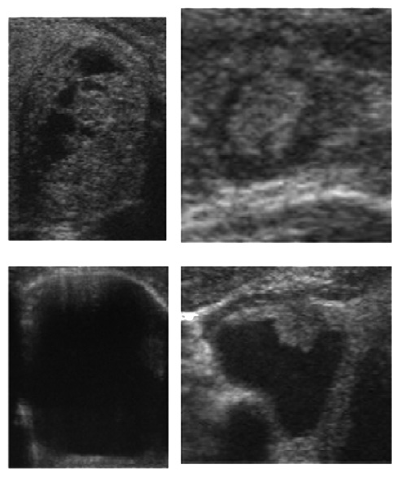
\includegraphics[width=0.40\textwidth]{2/figures/imagenes_ultrasonido_originales.png}
		\caption[Imágenes de ultrasonido de nódulos tiroideos]{Imágenes de ultrasonido de nódulos tiroideos. \\
		Fuente: \cite{pr_JERBI2023autoclassViTGAN}. \textit{Automatic classification of ultrasound thyroids images using vision transformers and generative adversarial networks}.}
		\label{2:fig210}
	\end{center}
\end{figure}
\end{comment}

\section{Marco Conceptual}
\subsection{Inteligencia Artficial}
Definir a la Inteligencia Artificial llega a ser complicado, esto debido a la dificultad que se tiene en definir lo que en verdad es inteligencia. Algunos grandes personajes pensaban de la inteligencia como la ambición, mientras que otros mencionaban a la imaginación como gran impulsador de la inteligencia. También lo consideraban como la capacidad de adaptarse a los cambios. Estas definiciones hacen pensar que no existe un consenso claro de lo que es la inteligencia, menos aun de la Inteligencia Artificial; sin embargo, en términos generales, se puede calificar de “Inteligencia Artificial” a todo aquel sistema sintético que muestra algún tipo de comportamiento “inteligente”. Esto quiere decir que se puede considerar como IA a todo a aquellos que simule los sentidos naturales como el visión o audición, incluso a la capacidad de algunos sistemas de aprender de forma autónoma según su entorno lo requiera. \parencite{bk_hurbans2020grokking}

\subsection{Perceptrón}
Inventado por Frank Rosenblatt en 1957, el Perceptrón es la unidad básica de una red neuronal e incluso es considerado como la más simple red neuronal artificial (ANN). \parencite{bk_geron2022handml}

El Perceptrón se muestra en la Figura \ref{2:fig207-2}.

\begin{figure}[H]
	\begin{center}
		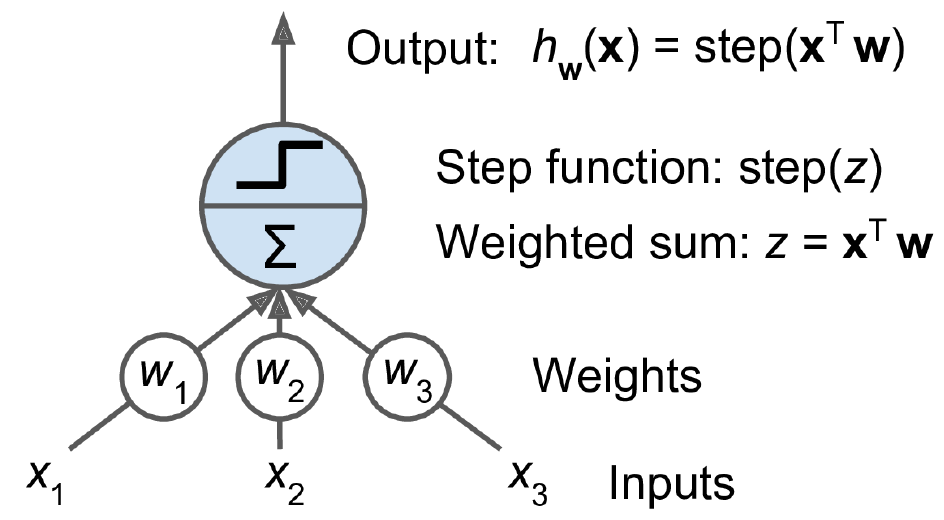
\includegraphics[width=0.75\textwidth]{2/figures/perceptron.png}
		\caption[Perceptrón]{Perceptrón. \\
		Fuente: \cite{bk_geron2022handml}. \textit{Hands-on machine learning with Scikit-Learn, Keras, and TensorFlow}.}
		\label{2:fig207-2}
	\end{center}
\end{figure}


\subsection{Perceptrón Multicapa}
Un Multi-Layer Perceptron (MLP) consiste en la unión de varios perceptrones, con la característica de estar organizados por capas. Existe una capa de entrada y otra de salida, todas las capas, a excepción de la salida, contiene una neurona adicional llamada bias. \parencite{bk_geron2022handml}

Una representación gráfica de un MLP se muestra en la Figura \ref{2:fig208}.

\begin{figure}[H]
	\begin{center}
		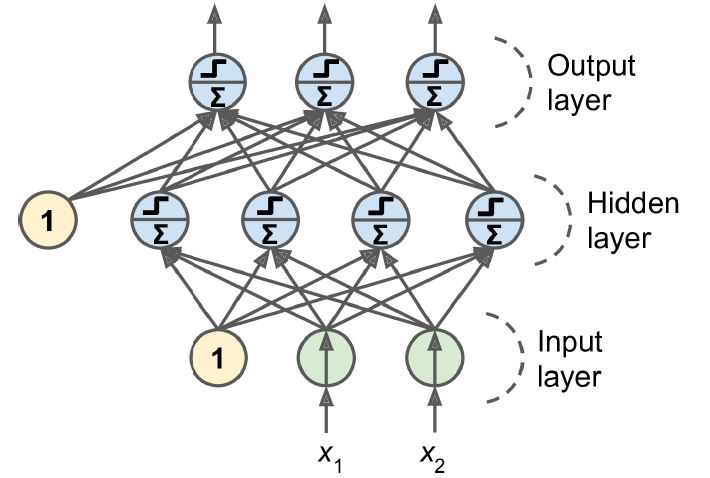
\includegraphics[width=0.77\textwidth]{2/figures/mlp.png}
		\caption[Perceptrón Multicapa]{Perceptrón Multicapa. \\
		Fuente: \cite{bk_geron2022handml}. \textit{Hands-on machine learning with Scikit-Learn, Keras, and TensorFlow}.}
		\label{2:fig208}
	\end{center}
\end{figure}


\subsection{Machine Learning}
El Aprendizaje Automático o Machine Learning es considerado como una ciencia y arte de dar instrucciones a una computadora para que pueda aprender por sí sola de una data. \parencite{bk_geron2022handml}

En la Figura \ref{2:fig209} se presenta el enfoque tradicional del Machine Learning.

\begin{figure}[H]
	\begin{center}
		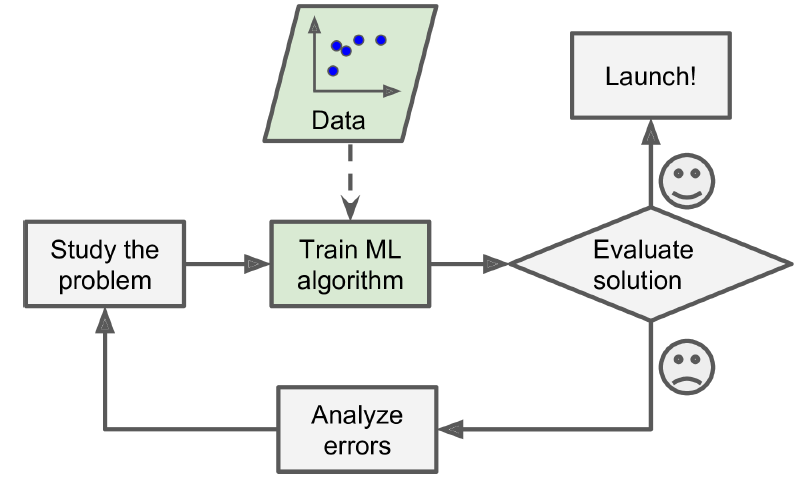
\includegraphics[width=0.75\textwidth]{2/figures/enfoque_ml.png}
		\caption[Enfoque del Machine Learning]{Enfoque del Machine Learning. \\
		Fuente: \cite{bk_geron2022handml}. \textit{Hands-on machine learning with Scikit-Learn, Keras, and TensorFlow}.}
		\label{2:fig209}
	\end{center}
\end{figure}

\begin{comment}

\subsection{Ecografía y las imágenes de ultrasonido}
Según \cite{pr_herrera2017diseimp}, la ecografía, que es una técnica de diagnóstico en donde se usan imágenes generadas por ultrasonido, es comúnmente desarrollado en las áreas de cardiología, ginecología, y otras más relacionadas. La popularidad de esta técnica se basa en la capacidad de las imágenes de alta calidad que se obtienen de este proceso, además de no ser un método invasivo o de radiación como muchos otros de su tipo.

Los sistema encargados de extraer las imágenes de ultrasonido son compuestos de distintas sensores que generan ondas de sonido para posteriormente analizar la respuesta de la interacción física con el campo de interés. Estas señales recibidas de regreso son digitalizados por una parte electrónica delantera que también transforman estos datos crudos en la imagen final. El funcionamiento de este proceso depende de la configuración de los sensores, el método usado para obtener las imágenes y las características de área de interés. \parencite{pr_camacho2022ultrasonicimg}

Algunas imágenes de ultrasonido de nódulos tiroideos se muestran en la Figura \ref{2:fig210}.

\begin{figure}[H]
	\begin{center}
		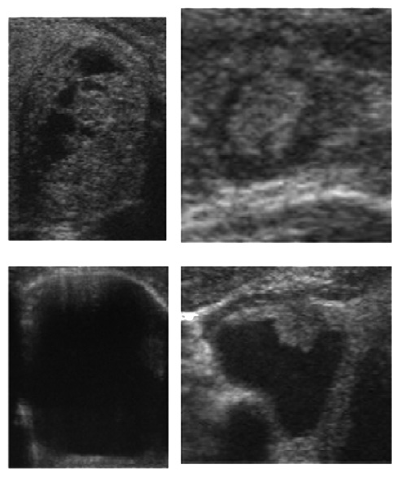
\includegraphics[width=0.40\textwidth]{2/figures/imagenes_ultrasonido_originales.png}
		\caption[Imágenes de ultrasonido de nódulos tiroideos]{Imágenes de ultrasonido de nódulos tiroideos. \\
		Fuente: \cite{pr_JERBI2023autoclassViTGAN}. \textit{Automatic classification of ultrasound thyroids images using vision transformers and generative adversarial networks}.}
		\label{2:fig210}
	\end{center}
\end{figure}


\subsection{Transfer Learning}
\cite{bk_geron2022handml} nos menciona que el Transfer Learning o Transferencia de Aprendizaje es un técnica usada en el campo de Deep Learning que permite el uso de algunas capas de un modelo ya definido y entrenado previamente en un nuevo modelo que necesite ser entrenado en una tarea similar al que se desarrolla el modelo original. Las capas destinadas al reuso son normalmente las más cercanas a la entrada o también conocidas como capas inferiores. El beneficio de usar esta técnica radica en dos puntos importantes: cantidad de datos requeridos y velocidad de entrenamiento del modelo; es decir, la cantidad de datos que se deben usar para entrenar un modelo de alto desempeño se reduce considerablemente, mientras que el tiempo requerido para terminar este proceso es menor comparándolo a si lo entrenaran desde cero.

Para que esta técnica funcione debidamente, las capas más cercanas a la salida, conocidas también como capas de alto nivel, deben ser reemplazadas, esto debido a que son más específicas de las tareas del modelo original. Esto también incluye a la capa final, ya que posiblemente no tenga la cantidad de salidas necesarias para completar satisfactoriamente la nueva tarea.

En la Figura \ref{2:fig211} se presenta de forma gráfica la técnica.

\begin{figure}[H]
	\begin{center}
		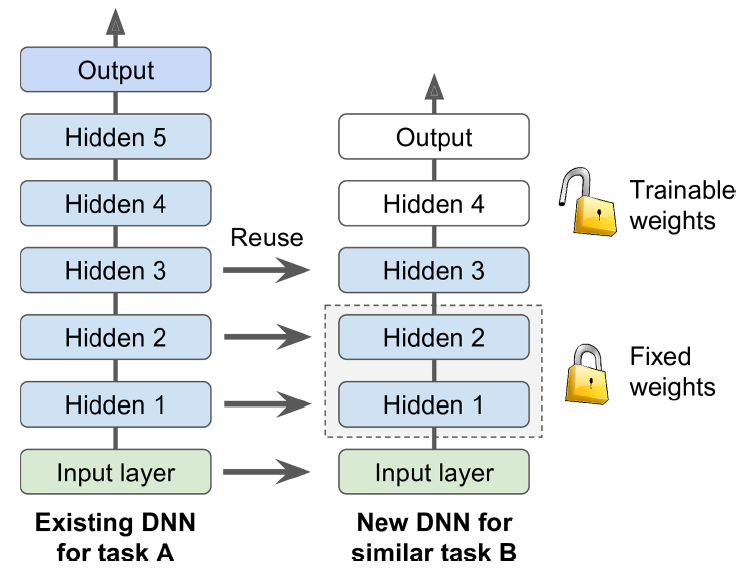
\includegraphics[width=0.70\textwidth]{2/figures/transfer_learning.PNG}
		\caption[Ejemplo de Transfer Learning]{Ejemplo de Transfer Learning. \\
		Fuente: \cite{bk_geron2022handml}. \textit{Hands-on machine learning with Scikit-Learn, Keras, and TensorFlow}.}
		\label{2:fig211}
	\end{center}
\end{figure}


\subsection{Data Augmentation}

Según \cite{bk_geron2022handml} el Aumento de Datos o Data Augmentation es una técnica de regularización que permite reforzar la cantidad de muestras en un conjunto de datos. Esto se realiza a través de la generación de nuevas instancias similares a los originales; es decir, las personas no deberían ser capaces de diferenciar una imagen generada de una del propio conjunto de datos.

Para generar estas nuevas muestras, normalmente se aplican diferentes transformaciones a las instancias del conjunto de datos original. Estas transformaciones pueden ser; por ejemplo, una simple rotación o recorte de la imagen, siempre y cuando no altere por completo su sentido como es el caso de voltear una imagen de texto de forma horizontal. 

El principal beneficio de esta técnica es que permite reducir el sobreajuste de los modelos entrenados. 

En la Figura \ref{2:fig212} se muestran algunas transformaciones que se pueden hacer al aplicar el Aumento de Datos. 

\begin{figure}[H]
	\begin{center}
		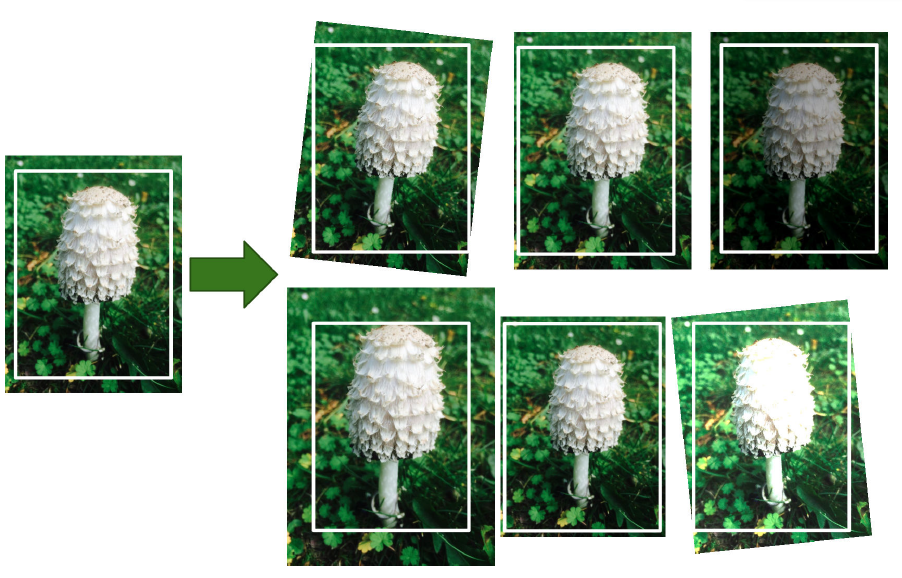
\includegraphics[width=0.85\textwidth]{2/figures/data_aug.PNG}
		\caption[Ejemplo de Data Augmentation]{Ejemplo de Data Augmentation. \\
		Fuente: \cite{bk_geron2022handml}. \textit{Hands-on machine learning with Scikit-Learn, Keras, and TensorFlow}.}
		\label{2:fig212}
	\end{center}
\end{figure}

\end{comment}

\section{Hipótesis}
\subsection{Hipótesis General}
HG: \newcommand{\HipotesisGeneral}{
A través del diseño de un modelo de Deep Learning se pre-diagnóstica los nódulos tiroideos a través de imágenes de ultrasonido.
}
\HipotesisGeneral


\subsection{Hipótesis Específicas}
\newcommand{\Hone}{
Las mejores características del conjunto de datos usadas para el proceso de entrenamiento y prueba permiten un mejor desarrollo del modelo de Deep Learning.
}
\newcommand{\Htwo}{
Las técnicas de preprocesamiento a aplicar a las imágenes de ultrasonido del conjunto de datos mejora el desempeño del modelo de Deep Learning.
}
\newcommand{\Hthree}{
Las métricas de evaluación de rendimiento de los modelos de Deep Learning logra una correcta comparación de modelos en la tarea de clasificación de imágenes de ultrasonido.
}
\newcommand{\Hfour}{
Las arquitecturas de Deep Learning con más alto desempeño en la clasificación de imágenes de ultrasonido demuestran superioridad frente a los demás modelos.
}

\begin{itemize}
	\item HE1: {\Hone}
	\item HE2: {\Htwo}
	\item HE3: {\Hthree}
	\item HE4: {\Hfour}
\end{itemize}

%\chapter{Metodología de la Investigación}



\section{Diseño de la investigación}

Según \cite{bk_sampieri2014metodologia}, los diseños experimentales se caracterizan por manipular y establecer relaciones de causa-efecto entre variables independientes y dependientes.

En esta investigación, se adopta un diseño experimental, ya que se busca establecer una relación entre las técnicas y modelos de aprendizaje profundo, específicamente redes neuronales convolucionales (CNN), y la detección automatizada de deterioros en pavimentos en Lima Metropolitana. Esto implica manipular los parámetros del modelo, así como las características de los datos utilizados, para analizar el impacto en la precisión y efectividad del sistema desarrollado.

\subsection{Alcance de la Investigación}

El alcance de la investigación incluye el diseño, entrenamiento y evaluación de un modelo CNN que permita clasificar imágenes de pavimentos de manera automática. Esto abarca:

Recolección y preparación del conjunto de datos de imágenes.
Implementación de técnicas de preprocesamiento y limpieza de datos.
Entrenamiento de modelos CNN con diferentes configuraciones.
Evaluación de la efectividad del modelo y comparación con métodos tradicionales de inspección visual.
El objetivo principal es contribuir a la optimización del mantenimiento vial, reduciendo costos y mejorando la seguridad vial mediante un sistema automatizado para la detección de deterioros.



\subsection{Tipo de la investigación}

Definido el diseño experimental, el tipo de investigación es experimental puro, ya que la variable independiente (técnicas y modelos de CNN) será manipulada para observar su impacto en la variable dependiente (precisión en la detección de deterioros). Esta manipulación incluye ajustes en los hiperparámetros del modelo, selección de características de las imágenes y técnicas de procesamiento de datos para optimizar los resultados.

Además, se realizarán iteraciones con diferentes configuraciones y subconjuntos del dataset, buscando maximizar métricas como precisión, recall y F1-score, indicadores clave del desempeño del modelo en la tarea de clasificación.

\subsection{Enfoque de la investigación}

De acuerdo con \cite{bk_sampieri2014metodologia}, el enfoque cuantitativo utiliza herramientas estadísticas y sigue un proceso estructurado y secuencial para medir variables y analizar relaciones entre ellas.

Esta investigación sigue un enfoque cuantitativo, ya que los resultados del modelo CNN serán evaluados mediante métricas estadísticas que permiten medir su rendimiento en la clasificación de imágenes de pavimentos. Las métricas empleadas, como precisión, recall, F1-score y curva ROC, servirán para evaluar de manera objetiva la efectividad del sistema propuesto.


\section{Población}

La población corresponde a imágenes de pavimentos urbanos en diversas condiciones de conservación, recolectadas en el contexto de la ciudad de Lima Metropolitana. Estas imágenes reflejan una variedad de tipos de deterioro comunes en pavimentos, como grietas y fisuras, que afectan la infraestructura vial.

\section{Muestra}

La muestra está constituida por un conjunto de 30,000 imágenes, clasificadas en dos categorías principales: con grietas y sin grietas. Estas imágenes fueron obtenidas por el autor Omoebamije Oluwaseun, utilizando un dron DJI Mavic 2 Enterprise para tomas aéreas y un smartphone para capturas a nivel del suelo. Las imágenes están en formato RGB, resolución 227x227 píxeles, y han sido etiquetadas previamente para su uso en tareas de clasificación mediante CNN.


\section{Operacionalización de Variables}

La operacionalización de las variables de esta investigación se describe en la Tabla \ref{tab:operacionalizacion_variables}, donde se especifican las dimensiones, indicadores y las fórmulas correspondientes para la medición de cada variable.

\begin{table}[H]
	\centering
	\caption{Operacionalización de variables para la Hipótesis General}
	\begin{tabular}{|p{4cm}|p{4cm}|p{4cm}|p{3cm}|}
	\hline
	\textbf{Variable} & \textbf{Definición Conceptual} & \textbf{Definición Operacional} & \textbf{Fórmula del Indicador} \\ \hline
	Implementación de un modelo automatizado basado en redes neuronales convolucionales (VI) & Uso de redes neuronales para la clasificación automatizada de deterioros en pavimentos. & Desarrollo, entrenamiento y validación de un modelo CNN para clasificar imágenes de pavimentos. & \(\text{Accuracy} = \frac{\text{TP} + \text{TN}}{\text{Total}}\) \\ \hline
	Calidad en la detección de deterioros en pavimentos (VD) & Grado de acierto en la identificación de daños en pavimentos. & Porcentaje de detección correcta de los deterioros en un conjunto de datos de prueba. & \(\text{Sensibilidad} = \frac{\text{TP}}{\text{TP} + \text{FN}}\) \\ \hline
	Eficiencia en el mantenimiento de vías (VD) & Optimización de recursos para reparar vías. & Reducción en el tiempo y los costos asociados con la reparación de vías, basada en la clasificación automatizada. & \(\text{Tasa de mejora} = \frac{\text{Antes} - \text{Después}}{\text{Antes}}\) \\ \hline
	Seguridad vial (VD) & Reducción de accidentes relacionados con deterioros en las vías. & Número de accidentes evitados debido al mantenimiento oportuno basado en detecciones automatizadas. & \(\text{Proporción} = \frac{\text{Accidentes evitados}}{\text{Total accidentes previos}}\) \\ \hline
	\end{tabular}
	\end{table}
	
\begin{table}[H]
	\centering
	\caption{Operacionalización de variables para la Hipótesis Específica 1}
	\begin{tabular}{|p{4cm}|p{4cm}|p{4cm}|p{3cm}|}
	\hline
	\textbf{Variable} & \textbf{Definición Conceptual} & \textbf{Definición Operacional} & \textbf{Fórmula del Indicador} \\ \hline
	Uso de redes neuronales convolucionales (VI) & Uso de algoritmos CNN para procesar imágenes y clasificarlas. & Entrenamiento de una red neuronal convolucional para clasificar imágenes en ``deterioradas'' y ``no deterioradas''. & \(\text{Precisión del modelo} = \frac{\text{Correctas}}{\text{Total clasificadas}}\) \\ \hline
	Precisión en la clasificación del estado de los pavimentos (VD) & Nivel de exactitud en la identificación del estado de los pavimentos. & Porcentaje de coincidencia entre la predicción del modelo y las etiquetas reales del conjunto de prueba. & \(\text{Accuracy} = \frac{\text{TP} + \text{TN}}{\text{Total}}\) \\ \hline
	\end{tabular}
\end{table}

		
\begin{table}[H]
	\centering
	\caption{Operacionalización de variables para la Hipótesis Específica 2}
	\begin{tabular}{|p{4cm}|p{4cm}|p{4cm}|p{3cm}|}
	\hline
	\textbf{Variable} & \textbf{Definición Conceptual} & \textbf{Definición Operacional} & \textbf{Fórmula del Indicador} \\ \hline
	Detección automatizada en tiempo real (VI) & Uso de modelos para identificar daños de manera inmediata. & Implementación de sistemas de detección que procesen datos en tiempo real para clasificar imágenes de pavimentos. & \(\text{Tiempo promedio} = \frac{\text{Total tiempo}}{\text{N imágenes}}\) \\ \hline
	Tiempo de respuesta para reparaciones (VD) & Lapso entre la identificación de daños y su reparación. & Medición en días u horas entre la detección del deterioro y la acción correctiva. & \(\text{Reducción} = \frac{\text{Tiempo antes} - \text{Tiempo después}}{\text{Tiempo antes}}\) \\ \hline
	Costos de mantenimiento a largo plazo (VD) & Gasto total asociado a reparaciones preventivas y correctivas en un periodo. & Comparación de los costos acumulados entre métodos tradicionales y el sistema automatizado. & \(\text{Diferencia} = \text{Costo Tradicional} - \text{Costo Automatizado}\) \\ \hline
	\end{tabular}
\end{table}
			
\begin{table}[H]
	\centering
	\caption{Operacionalización de variables para la Hipótesis Específica 3}
	\begin{tabular}{|p{4cm}|p{4cm}|p{4cm}|p{3cm}|}
	\hline
	\textbf{Variable} & \textbf{Definición Conceptual} & \textbf{Definición Operacional} & \textbf{Fórmula del Indicador} \\ \hline
	Priorización de zonas más deterioradas (VI) & Identificación de áreas críticas para reparación con base en el nivel de daño. & Uso del modelo CNN para asignar prioridad a las áreas con mayores índices de deterioro. & \(\text{Índice de prioridad} = \frac{\text{Deterioro}}{\text{Área total}}\) \\ \hline
	Eficiencia en la asignación de recursos (VD) & Optimización del uso de personal, materiales y tiempo en función de las prioridades detectadas. & Comparación de recursos asignados antes y después de implementar el modelo automatizado. & \(\text{Tasa de eficiencia} = \frac{\text{Producción después}}{\text{Recursos después}}\) \\ \hline
	\end{tabular}
\end{table}
				

\noindent
Las fórmulas de los indicadores son las siguientes:
\begin{itemize}
    \item \textbf{Precisión (Accuracy)}: Relación entre predicciones correctas y el total de predicciones. 
    \[
    Accuracy = \frac{TP + TN}{TP + TN + FP + FN}
    \]
    \item \textbf{Recall (Sensibilidad)}: Proporción de verdaderos positivos respecto a todas las muestras positivas. 
    \[
    Recall = \frac{TP}{TP + FN}
    \]
    \item \textbf{F1-score}: Media armónica de precisión y recall. 
    \[
    F1 = 2 \cdot \frac{Precision \cdot Recall}{Precision + Recall}
    \]
    \item \textbf{ROC-AUC}: Área bajo la curva ROC, calculada mediante integración numérica de los valores de TPR y FPR a diferentes umbrales.
    \item \textbf{Eficiencia computacional}: Evaluada a través del tiempo de entrenamiento (en segundos o minutos) y la memoria utilizada (en GB o MB).
\end{itemize}


\section{Técnicas de Recolección de Datos}

En la presente investigación, las técnicas de recolección de datos empleadas son las siguientes:

\begin{itemize}
    \item \textbf{Obtención del dataset:} Se utilizaron fuentes secundarias para recolectar un conjunto de datos previamente elaborado, específicamente el dataset titulado *Concrete and Pavement Crack Dataset*. Este dataset contiene imágenes de superficies de concreto y pavimento clasificadas en dos categorías: con grietas y sin grietas. Las imágenes fueron recopiladas mediante el uso de un dron DJI Mavic 2 Enterprise y un smartphone, con una resolución de 227 x 227 píxeles en formato RGB.
    \item \textbf{Validación del dataset:} Antes de su uso, el dataset fue revisado para garantizar que todas las imágenes cumplan con los estándares de calidad necesarios, verificando la clasificación correcta de las categorías (crack y non-crack).
    \item \textbf{Preparación de los datos:} Se realizaron procesos de preprocesamiento para adaptar los datos al entrenamiento del modelo de redes neuronales convolucionales (CNN), incluyendo la normalización, el cambio de tamaño de las imágenes y la división del dataset en conjuntos de entrenamiento, validación y prueba.
\end{itemize}

Estas técnicas aseguran la correcta disposición y calidad de los datos para el análisis y entrenamiento del modelo.


\section{Técnicas para el Procesamiento y Análisis de Información}

El procesamiento y análisis de la información se llevó a cabo mediante el uso de técnicas basadas en aprendizaje profundo y análisis estadístico. Los pasos seguidos fueron los siguientes:

\begin{itemize}
    %%falta item de adquisición
	\item \textbf{Adquisición del dataset:} El conjunto de datos utilizado para entrenar y evaluar el modelo será obtenido mediante una recopilación de imágenes de pavimentos en Lima Metropolitana, capturadas a través de drones, cámaras móviles o bases de datos públicas. Estas imágenes serán procesadas y etiquetadas manualmente para su clasificación en diferentes tipos de deterioros.
	\item \textbf{Preprocesamiento:} Las imágenes fueron sometidas a procesos de normalización y aumento de datos (\textit{data augmentation}) para mejorar la calidad y diversidad del dataset.
    \item \textbf{Entrenamiento del modelo:} Se entrenaron redes neuronales convolucionales (CNN) utilizando el conjunto de entrenamiento del dataset. Durante este proceso, se ajustaron los hiperparámetros clave, como la tasa de aprendizaje y el tamaño del lote.
    \item \textbf{Validación y ajuste:} Se utilizó el conjunto de validación para ajustar los hiperparámetros del modelo y prevenir el sobreajuste.
    \item \textbf{Evaluación:} El modelo final fue evaluado con el conjunto de prueba utilizando métricas de rendimiento como precisión (\textit{accuracy}), sensibilidad (\textit{recall}), y F1-score.
\end{itemize}

El flujo del proceso se ilustra en el Diagrama %\ref{fig:procesamiento_analisis}.

\begin{figure}[H]
	\begin{center}
		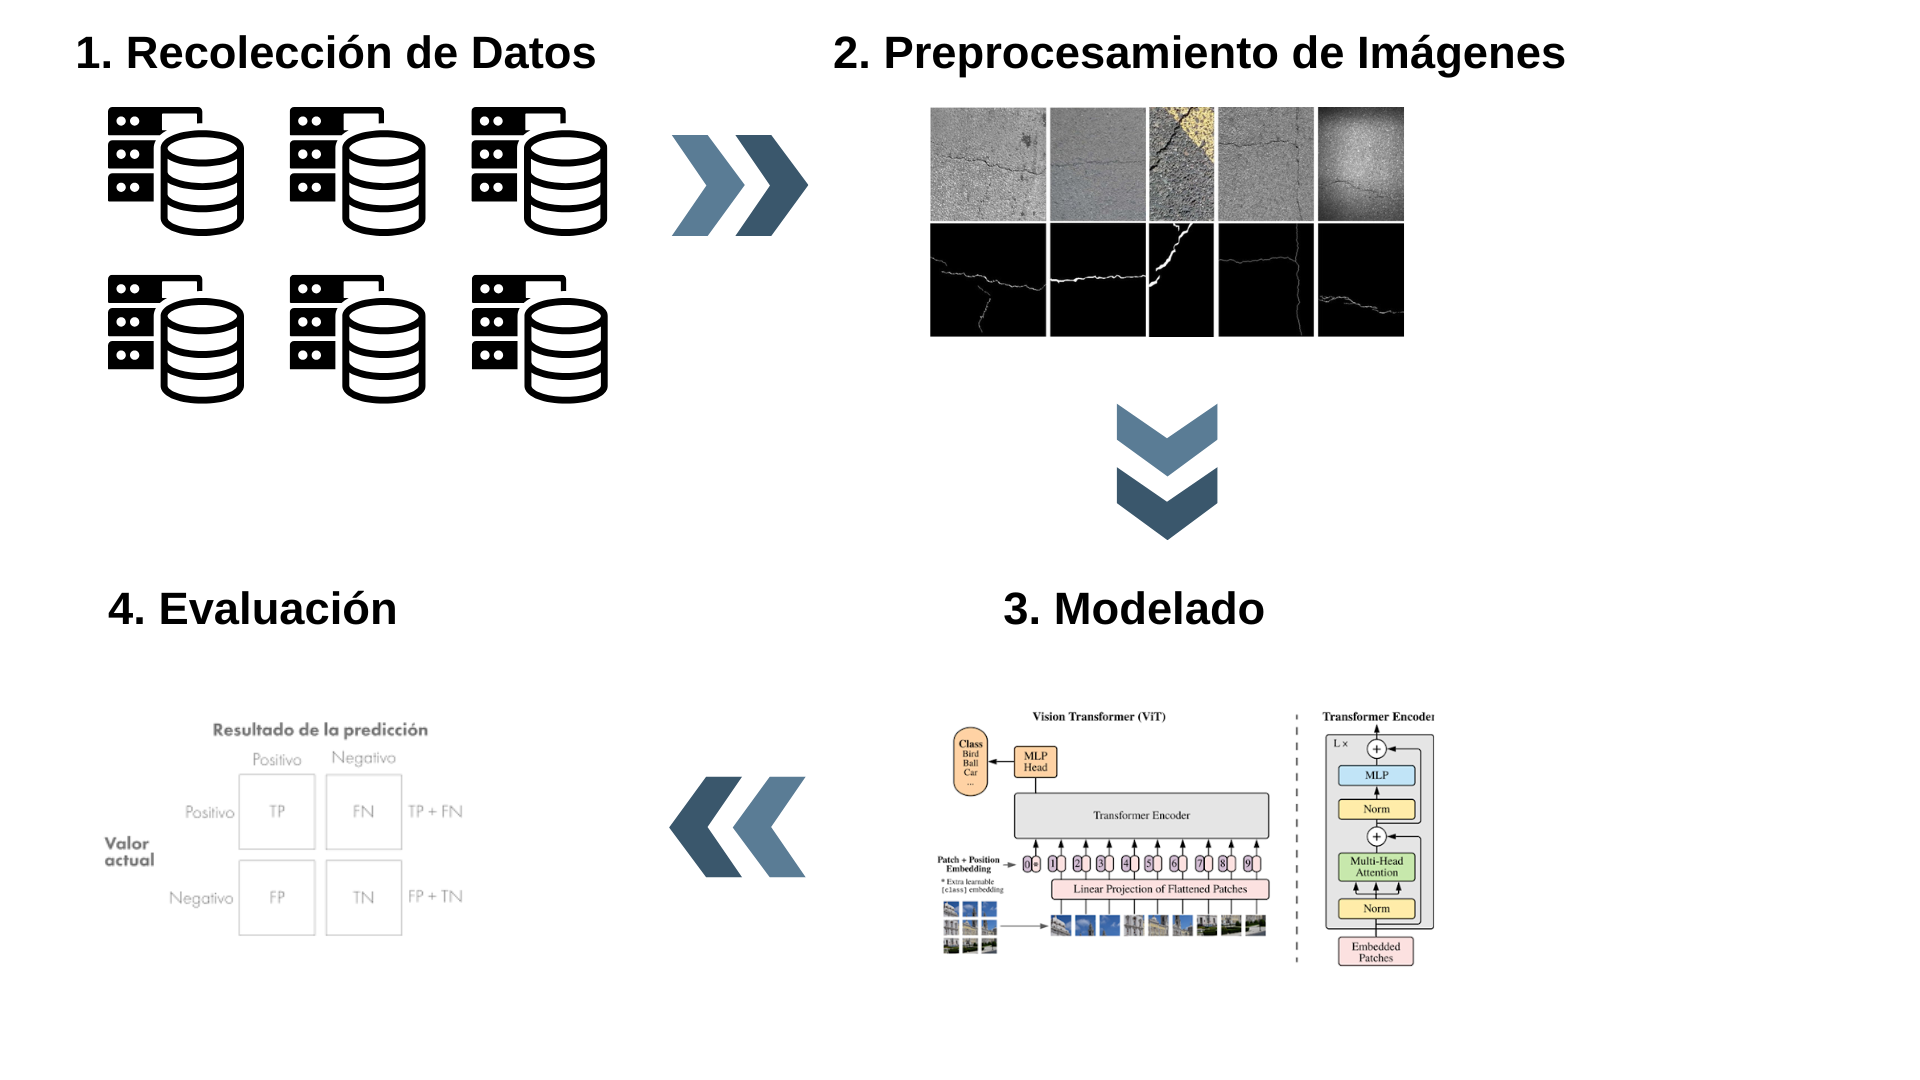
\includegraphics[width=1.00\textwidth]{2/figures/diagrama.png}
		\caption[Diagrama del procesamiento y análisis de la información]{Diagrama del procesamiento y análisis de la información. \\
		Fuente: Elaboración propia.}
		%\label{3:fig301}
	\end{center}
\end{figure}





%\section{Metodología de Implementación de la Solución}












\begin{comment}
La metodología por seguir para implementar un modelo de Deep Learning está basado en gran medida en el conocido ciclo de vida de desarrollo de modelos de Inteligencia Artificial, del cual gran parte de los antecedentes mostrados anteriormente siguen con algunas variaciones. 

En el presente caso, se pretende desarrollar un modelo de Deep Learning capaz de brindar ayuda en el diagnóstico médico; por tal motivo, se optó por basar metodología de esta investigación en la de \cite{pr_monroy2021disvc}, modificándolo en cierta medida en el contexto de nódulos tiroideos e imágenes de ultrasonido. En la Figura \ref{3:fig301} se presenta de forma gráfica la metodología a seguir.

\begin{figure}[H]
	\begin{center}
		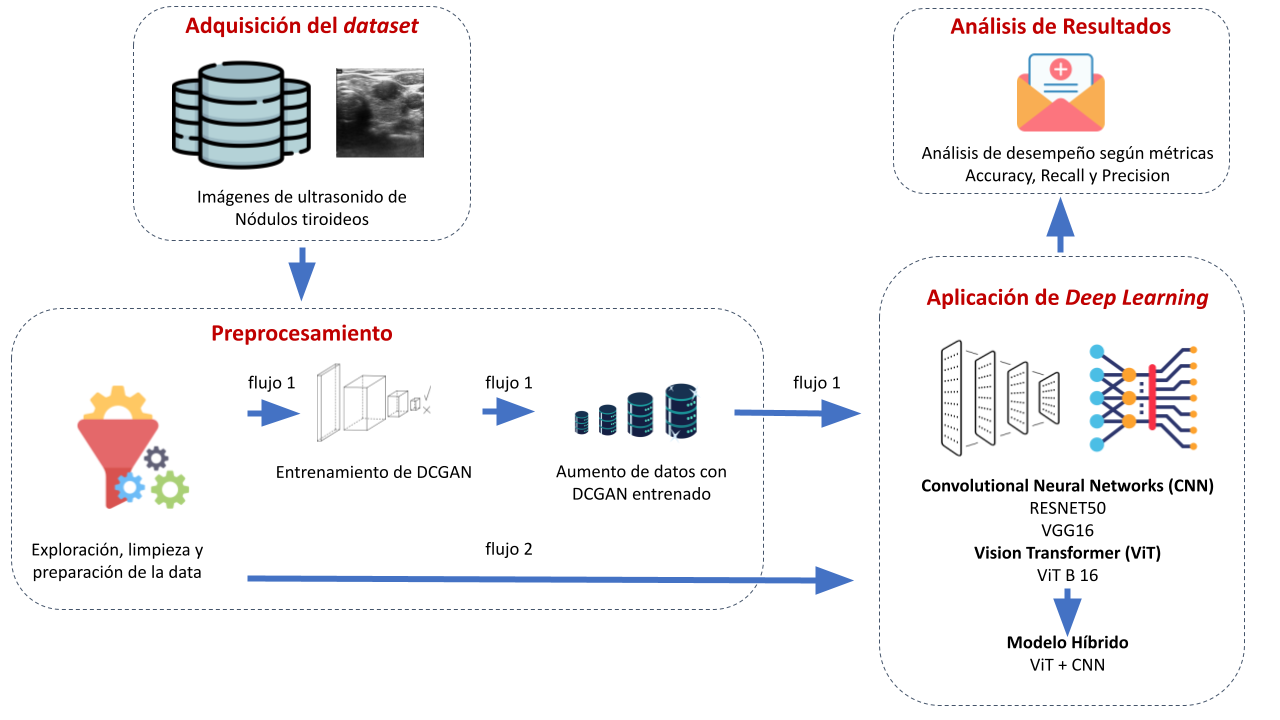
\includegraphics[width=1.00\textwidth]{3/figures/metod_classthy1.png}
		\caption[Metodología de implementación]{Metodología de implementación. \\
		Fuente: Elaboración propia.}
		\label{3:fig301}
	\end{center}
\end{figure}

La adquisición del conjunto de datos, es decir, imágenes de ultrasonido, consiste en la búsqueda y revisión de las bases de datos sobre imágenes de nódulos tiroideos, donde finalmente se seleccionará y descargará la de mayor utilidad. La base de datos debe cumplir con ciertos requerimientos para realizar un posterior entrenamiento del modelo que otorgue buenos resultados. Las imágenes deben ser debidamente etiquetadas según el carácter del nódulo al que representen, es decir, se debe indicar si cada una de las imágenes pertenece a la categoría benigno o maligno. Además, para evitar discrepancias entre calidad de imágenes en futuras evaluaciones, el conjunto de datos debe poseer imágenes de distintas instituciones de salud y de distintas calidades. Esto permitirá que el modelo entrenado no dependa de la una alta o baja calidad de las imágenes para realizar una correcta predicción. Finalmente, la cantidad de datos debe ser relativamente alta con el fin de aumentar la capacidad de generalización del modelo y evitar posibles sobreajustes o bajo rendimiento.  

En la etapa de preprocesamiento, se realizará en primera instancia una exploración del conjunto de datos con el fin de entender su composición y las características a mejorar; por ejemplo, un posible desbalanceo de clases o presencia de imágenes corruptas o sin etiquetar. Posteriormente, se realizará limpieza datos en caso de imágenes corruptas o de nula utilidad. Además, se usarán técnicas de Aumento de Datos en la situación de desbalanceo de datos, con el fin de evitar una baja generalización y sobreajuste en la clase mayoritaria. Además, se aplicará un redimensionamiento y normalización en las imágenes destinadas al entrenamiento del modelo con el objetivo de reducir la complejidad computacional y así obtener menor tiempo de ejecución.

Una vez se tenga la data ya preprocesada, una parte de este se usará para el entrenamiento de modelos de Deep Learning. Inicialmente, se planea usar algunos de los diversos tipos y arquitecturas de Redes Neuronales Convolucionales (CNN), específicamente los más utilizados en este tipo de tareas como lo son VGG y ResNet, pues son ideales para la extracción de características de las imágenes, facilitando así el proceso final de clasificación. Además, se desarrollarán modelos basados en arquitecturas de Vision Transformer debido al potencial que han demostrado en anteriores investigaciones. Finalmente, también se realizará el desarrollo de modelos híbridos de CNN con Vision Transformer. %similares a los descritos por \cite{pr_JERBI2023autoclassViTGAN}.

Cada uno de los modelos será probado en la parte restante de la data, específicamente en la data de prueba o test. De aquí se obtendrán las predicciones de los modelos clasificando las imágenes en benigno (0) o maligno (1).

\section{Metodología para la Medición de Resultados de la Implementación}

Los resultados obtenidos de la clasificación de los modelos previamente entrenados deberán ser evaluados para una correcta elección final. 

Antes de presentar las métricas a usar, es necesario conocer a la matriz de confusión y las partes que lo conforman, pues servirá como base para entenderlas. 

Según \cite{ws_izco2018bdcp} la matriz de confusión es una herramienta que permite ver de forma más clara el rendimiento de nuestro modelo. Este se presenta en la Figura \ref{3:fig302}.

\begin{figure}[H]
	\begin{center}
		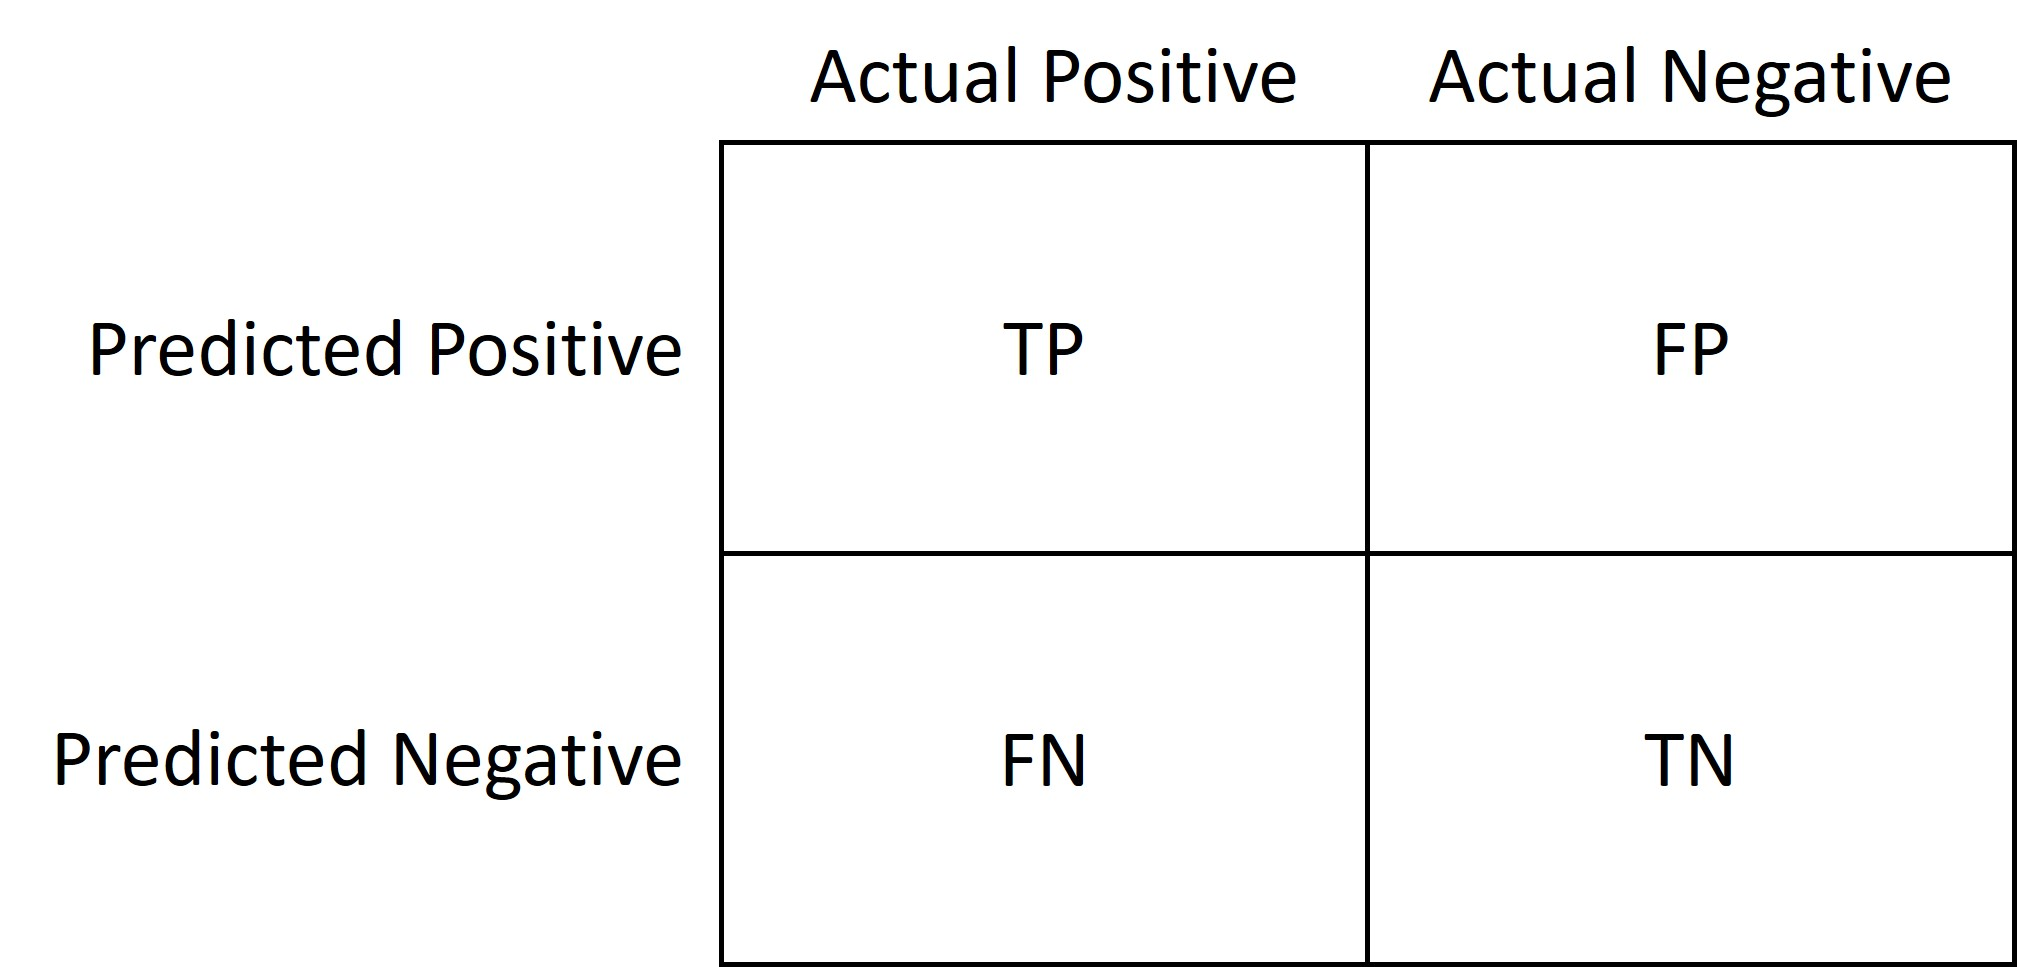
\includegraphics[width=0.75\textwidth]{3/figures/conf_matrix.jpg}
		\caption[Matriz de Confusión]{Matriz de Confusión. \\
		Fuente: Elaboración propia.}
		\label{3:fig302}
	\end{center}
\end{figure}

La matriz consta de cuatro partes importantes: TP, FP, FN y TN. Estos serán usados para presentar las fórmulas de las métricas más adelante. El primero (TP o true positive) se refiere a la cantidad de observaciones que se han predicho como positivos y que en verdad sí son positivos; por el contrario, FP (false positive) se refiere a aquellas predicciones dadas como positivos, pero en verdad son negativos. FN (false negative) es la cantidad de observaciones predichas como negativas; sin embargo, estas en realidad son positivas. Finalmente, TN (true negative) es la cantidad de observaciones predichas como negativas y que en realidad son también negativas.

A continuación, se presenta las métricas para medir el desempeño de la clasificación del modelo.

El accuracy representa aquella proporción del total de predicciones que se ha obtenido correctamente \parencite{ws_izco2018bdcp}. Este se calcula a través de la siguiente fórmula 1.

%\begin{equcaption}[!ht]
\begin{equation}\label{eq:accuracy}
\phantomsection
accuracy=\frac{TP+TN}{TP+TN+FP+FN}
\end{equation}
\myequations{Fórmula para calcular el accuracy}

El recall representa la proporción de solo los positivos reales predichos de manera acertada \parencite{ws_izco2018bdcp}. Se calcula con la siguiente fórmula.

%\begin{equcaption}[!ht]
\begin{equation}\label{eq:recall}
\phantomsection
recall=\frac{TP}{TP+FN}
\end{equation}
\myequations{Fórmula para calcular el recall}

Precision representa aquella proporción de lo predicho positivamente que es positiva \parencite{ws_izco2018bdcp}. Se calcula con la fórmula a continuación.

%\begin{equcaption}[!ht]
\begin{equation}\label{eq:precision}
\phantomsection
precision=\frac{TP}{TP+FP}
\end{equation}
\myequations{Fórmula para calcular el precision}

\begin{landscape}
	\section{Cronograma de actividades y presupuesto}
	Se propuso un cronograma para la investigación. Conforma desde el inicio hasta ser terminada con la sustentación final planeada para mediados del año 2024. Este se presneta en la Figura \ref{3:fig303}.

	\begin{figure}[!ht]
		\begin{center}
			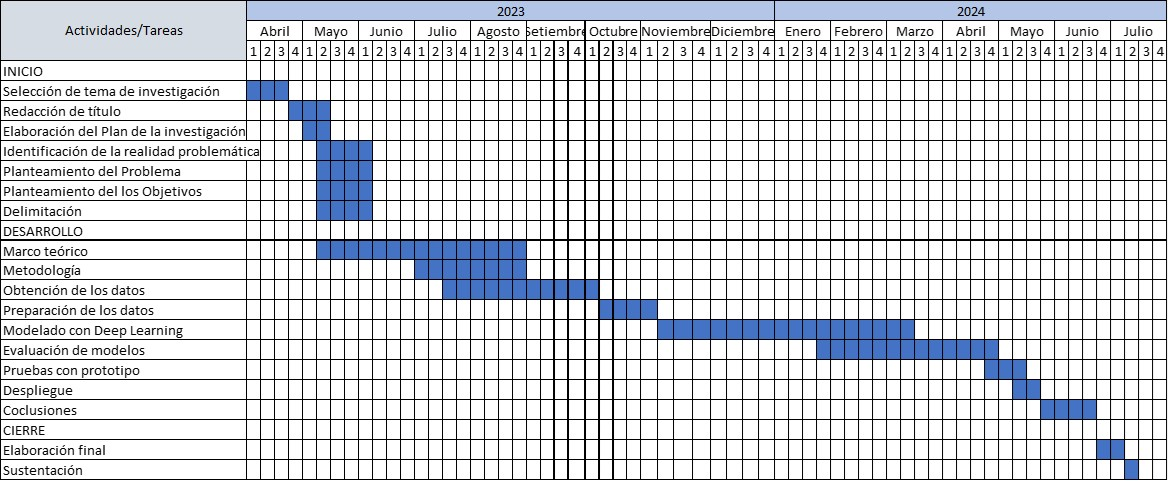
\includegraphics[width=1.50\textwidth]{3/figures/cronograma_tesis_thyr.jpg}
			\caption[Cronograma de actividades]{Cronograma de actividades.\\
				Fuente: Elaboración propia.}
			\label{3:fig303}
		\end{center}
	\end{figure}
	
\end{landscape}

Además, se determinó el presupuesto necesario para la elaboración completa de la investigación. Este se presenta en la Tabla \ref{3:table1}.

\begin{table}[H]
	\caption[Presupuesto]{Presupuesto.}
	\label{3:table1}
	\centering
	\small
	\begin{tabular}{llll}
		\specialrule{.1em}{.05em}{.05em}
		{Grupo} & {Item} & {Costo (soles)} & {Subtotal} \\
		\specialrule{.1em}{.05em}{.05em}
		\multirow{2}{4cm}{Recursos materiales} & {Laptop} & {S/ 6,500.00} & {} \\
		{} & {Materiales de escritorio} & {S/ 100.00} & {S/ 6,600.00} \\
		\cline{1-4}
		\multirow{2}{4cm}{Software y trámites} & {Matrícula de Trabajo de Tesis II} & {S/ 375.00} & {} \\ % & {Reserva de tema} & {S/ 2,700.00} & {} \\
		{} & {Cuotas de Trabajo de Tesis II} & {S/ 1,044.00} & {} \\
		%{} & {Derecho de inscripción} & {S/ 800.00} & {} \\
		%{} & {Derecho de sustentación} & {S/ 1,500.00} & {} \\
		{} & {Software} & {S/ 50.00} & {} \\
		{} & {Renta de servidor en la nube} & {S/ 224.15} & {S/ 1,693.15} \\ % & {S/ 5,274.15} \\
		\cline{1-4}
		\multirow{2}{4cm}{Extras} & {Consultorías} & {S/ 100.00} & {} \\
		{} & {Movilidad} & {S/ 200.00} & {S/ 300.00} \\
		\specialrule{.1em}{.05em}{.05em} 
		{} & {Total} & {} & {S/ 8,593.15} \\ % & {S/ 12,174.15} \\
		\specialrule{.1em}{.05em}{.05em}
	\end{tabular}
	\begin{flushleft}	
		\small Fuente: Elaboración propia.
	\end{flushleft}
\end{table}

\end{comment}


%\begin{comment}
\chapter{Desarrollo de la Solución}
En el presnete capítulo se describe las herramientas y procesos de desarrollo del modelo de Deep Learning.

\section{Determinación y evaluación de alternativas de solución}

En esta sección se presentarán las arquitecturas base CNN y ViT que se usarán en el entrenamiento de los modelos de Deep Learning para la tarea de clasificación de nódulos tiroideos a través de imágenes de ultrasonido. Además, también se introducirá la idea de modelo híbrido que junta las capacidades de extracción de características de los CNN con la actualmente popular arquitectura ViT.

En el grupo de modelos CNN, se tiene en primera instancia a la arquitectura VGG16, ya presentada anteriormente en el Capítulo 2.Este modelo posee 16 capas de profundidad junto con un tamaño de 3 x 3 en los filtros. Se ha reconocido que VGG16, y las arquitecturas VGGNet en general, poseen una alta capacidad de generalización, lo cuál lo vuelve ideal para tareas de clasificación distintas a los que originalmente fue entrenado. \parencite{pr_simonyan2015vdcn}

En segundo lugar, también parte del grupo de modelos CNN, se tiene a ResNet 50, también ya presentado inicialmente en el Capítulo 2. Esta arquitectura introdujo el concepto de redes residuales que permitieron obtener de manera más optimizada un mayor desempeño en arquitecturas de alta profundidad. \parencite{pr_he2016deepres} La versión de ResNet usada en esta investigación fue la de 50 capas de profundidad.

En el conjunto de modelos ViT, el usado en la presente investigación fue la ViT-Base con patch de tamaño 16 x 16.

Los modelos ViT también ya fueron presentados en el Capítulo 2.

Esta arquitectura, basada en los originales Transformers, ha demostrado tener mejor desempeño en tareas de clasificación comparado a los modelos basados en CNNs, aunque ciertamente con una mayor necesidad de datos de entrenamiento.

En la Figura \ref{2:fig206}, ya se muestra la forma de la arquitectura del modelo ViT. Cabe volver a resaltar que la versión del modelo ViT utilizado es el Base que consta de 86 millones de parámetros y recibe patch de tamaño 16 x 16.

Finalmente, el último modelo presente en la investigación es uno que combina la capacidad de los CNN y los ViT para obtener un modelo híbrido.

Este modelo utiliza al CNN como backbone que alimentará los features extraídos en forma de patch de tamaño 1 x 1 al modelo ViT. Para lograr esto se es necesario quitar el cabezal clasificador de la arquitectura CNN, pues esta tarea ya será desarrollada por el propio ViT.

Debido a las limitaciones de tiempo y recursos, solamente se desarrollará dos modelos híbridos con aquellos CNN de mejor desempeño en los entrenamientos iniciales.

Cabe destacar que este modelo híbrido fue inspirado por el trabajo presentado por \cite{pr_JERBI2023autoclassViTGAN}. A continuación se presenta la Figura \ref{4:fig101}, donde se muestra la arquitectura híbrida.

\begin{figure}[H]
	\begin{center}
		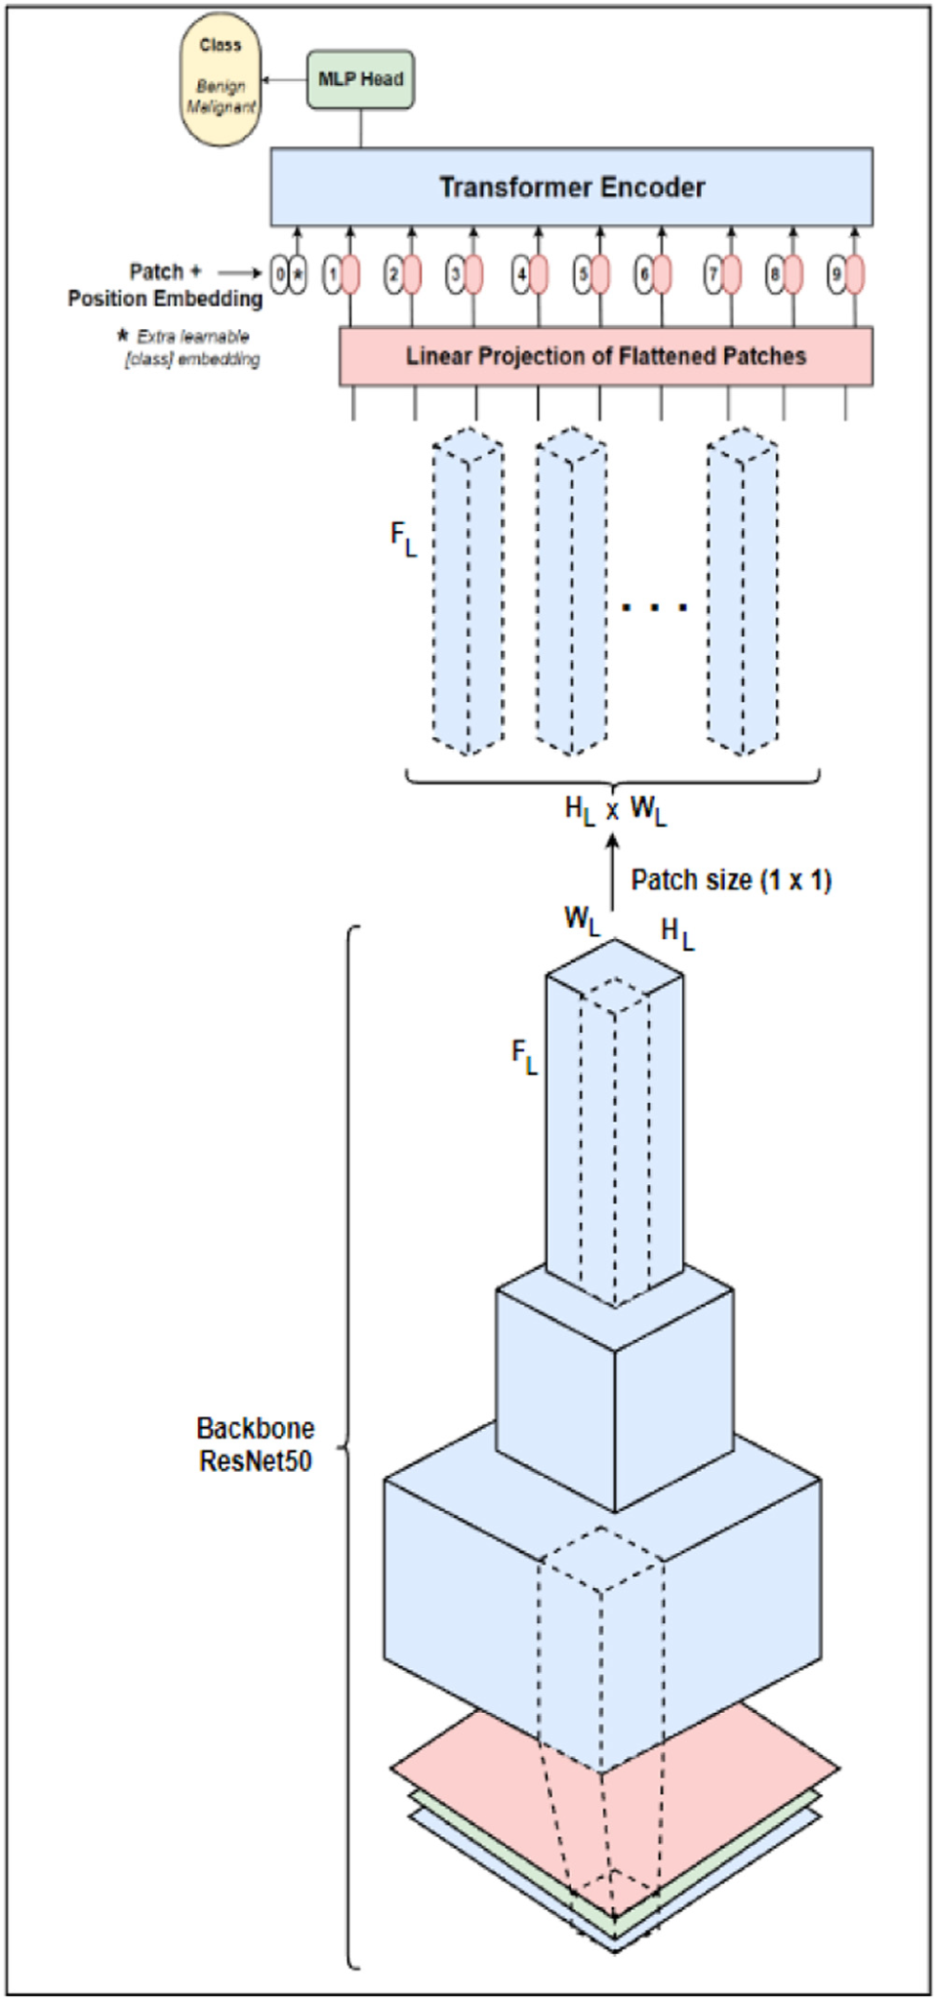
\includegraphics[width=0.60\textwidth]{4/figures/hybrid_arc.png}
		\caption[Arquitectura híbrida CNN + ViT]{Arquitectura híbrida CNN + ViT. \\
		Fuente: \cite{pr_JERBI2023autoclassViTGAN}. \textit{Automatic classification of ultrasound thyroids images using vision transformers and generative adversarial networks}.}
		\label{4:fig101}
	\end{center}
\end{figure}

\section{Propuesta solución}

\subsection{Planeamiento y descripción de Actividades}

La metodología descrita en el capítulo anterior consta de tres etapas principales: adquisición de datos, preprocesamiento de los datos y la aplicación de Deep Learning; es decir, el entrenamiento de los diferentes tipos de algoritmos. En la siguiente parte de esta investigación se procederá describir las actividades necesarias para desarrollar y completar cada una de estas etapas para, finalmente, obtener los resultados de cada uno de los modelos entrenados.

La metodología inicia con la adquisición del conjunto de datos necesario para realizar el entrenamiento de los modelos de Deep Learning. Este consta de las siguientes actividades.

\textbf{Actividad 1: Buscar y revisar bases de datos sobre imágenes de ultrasonido de nódulos tiroideos}
\\
En esta actividad se investigarán y analizarán aquellos conjunto de datos que cumplan con las características básicas requeridas: poseer imágenes de ultrasonido de nódulos tiroideos benignos y malignos.

\textbf{Entregable:} Diversos conjuntos de datos de imágenes de ultrasonido de nódulos tiroideos benignos y malignos.
\\

\textbf{Actividad 2: Filtrado de los conjuntos de datos}
\\
El conjunto de datos seleccionado debe cumplir con los siguientes requerimientos: las imágenes deben poseer información del carácter del nódulo; en otras palabras, se debe tener información sobre la imagen cada imagen de ultrasonido donde se indique si se está ante un nódulo de carácter benigno o maligno. Otra importante característica, necesaria para evitar obtener completamente distintos resultados en futuras investigaciones, es la fuente de origen de las imágenes del conjunto de datos, ya que este debe poseer imágenes de diferentes instituciones y herramientas. Esta característica permitirá a los modelos a entrenar tener la capacidad de afrontar distintas calidades y tipos de imágenes de ultrasonido. La última característica radica en la cantidad de las imágenes, ya que el conjunto de datos debe poseer una moderada cantidad de datos que permitan a los modelos interpretar mejor las imágenes de ultrasonido, y así finalmente aumentar la capacidad de generalización del modelo.

\textbf{Entregable:} Conjunto de datos de imágenes de ultrasonido de nódulos tiroideos benignos y malignos que cumple con todas las características requeridas.
\\
En la etapa de preprocesamiento, necesaria para realizar un correcto entrenamiento de los modelos de Deep Learning, se realizará un análisis y limpieza de los datos, además, se pasará por un proceso de preparamiento de los datos para facilitar el flujo de los datos a través de los de los modelos a entrenar. Esta etapa consta de dos flujos, donde uno de estos incluye el Aumento de Datos con el modelo DCGAN; mientras que el otro, evita el paso por este proceso debido a la fiabilidad de este tipo de red para generar datos que puedan ser útiles para el entrenamiento de los modelos. Ambos flujos constan de las tres primeras actividades descritas a continuación.

\textbf{Actividad 1: Explorar características del conjunto de datos}
\\
Se inicia con la exploración del conjunto de datos seleccionado, extrayendo gráficas y tablas que muestren su composición y características, permitiendo así determinar qué técnicas se podrían aplicar para mejorar las flaquezas del conjunto de datos. Aquí se puede obtener información sobre la necesidad o no de aplicar el Aumento de Datos a una clase minoritaria si lo hubiera.

\textbf{Entregable:} Gráficas y tablas de características y composición del conjunto de datos.
\\

\textbf{Actividad 2: Filtrar y organizar imágenes poco útiles del conjunto de datos}
\\
Se realizará un filtrado de aquellas imágenes corruptas, atípicas o sin etiqueta, dejando solo en el conjunto de datos a aquellas de mayor utilidad, al mismo tiempo que se reorganiza en un nuevo formato de ficheros para facilitar su posterior carga a los modelos de Deep Learning.

\textbf{Entregable:} Conjunto de datos organizados y sin imágenes corruptas, atípicas o sin etiquetas.
\\

\textbf{Actividad 3: Redimensionar, normalizar y dividir los datos según los requerimientos para cada modelo de Deep Learning}
\\
Inicialmente se aplicará a cada imagen un redimensionamiento y normalización según se vea conveniente, esto con el fin de evitar mayor complejidad computacional y reducir los tiempos de ejecución de los modelos. Luego se hará una división del conjunto de datos total en data de entrenamiento, validación y prueba.

\textbf{Entregable:} Conjunto de datos de entrenamiento, validación y prueba preprocesados.
\\
El segundo flujo de la metodología, al evitar el proceso de Aumento de Datos, obvia la siguiente actividad y continúa directamente en la siguiente etapa.

\textbf{Actividad 4: Mejorar composición del conjunto de datos}
\\
El Aumento de Datos se debe utilizar en caso de desbalance de clases en el conjunto de datos con el objetivo de aumentar la capacidad de generalización del modelo y evitar su sobreajuste.

Debido a las características que determinan si una imagen de ultrasonido es benigno o maligno (forma, orientación, tamaño y nivel de brillo), usar las técnicas comunes de Aumento de Datos de hacer diferentes transformaciones en las imágenes originales de forma aleatorio, no tendría sentido. Por este motivo, en esta actividad, se entrenará un modelo DCGAN personalizado que logre aprender la distribución de las imágenes reales y pueda generar posteriormente imágenes sintéticas. El entrenamiento de este modelo se realizará a través del conjunto de datos de entrenamiento obtenido de la anterior actividad, seleccionando aquellos pertenecientes a la clase de minoritaria.

Ya con el modelo entrenado, este será utilizado para generar y aumentar la cantidad de datos final para la clase minoritaria en la data de entrenamiento.

\textbf{Entregable:} Conjunto de datos con ambas clases balanceadas.
\\
Una vez se termina el preprocesamiento y se obtiene la data final, se continúa con el entrenamiento y validación de modelos de Deep Learning, seguido de una prueba final con la data respectiva. Esta etapa se divide en las siguientes actividades.

\textbf{Actividad 1: Seleccionar algoritmos a entrenar según usos y resultados de las investigaciones presentadas en los antecedentes}
\\
Se revisará aquellas arquitecturas utilizadas en las investigación mencionadas en el Capítulo 2. De todas las recolectadas, se seleccionarán las de mejor desempeño y de mayor presencia.

\textbf{Entregable:} Arquitecturas de Deep Learning ideales para la tarea de clasificación de imágenes de ultrasonido de nódulos tiroideos.
\\

\textbf{Actividad 2: Entrenar y probar los modelos de Deep Learning previamente definidos}
\\
Se realizará el entrenamiento de cada uno de las diferentes arquitecturas con configuraciones establecidas por anteriores investigaciones. También se aplicarán dos técnicas por separado para este proceso: Transfer Learning y Fine Tuning. Además, en cada época de entrenamiento de todos los modelos, se usará el conjunto de datos de validación para verificar el avance de la capacidad predictiva de los modelos.

Finalmente, cada uno de estos modelo será puesto a prueba en el conjunto de datos restantes (data de prueba), así finalmente se obtendrán las métricas correspondientes que permitirán luego realizar el análisis de desempeño.

\textbf{Entregable:} Modelos CNN y ViT entrenados. Métricas de cada uno de los modelos.
\\

\textbf{Actividad 3:  Definir modelos híbridos entre ViT y CNN}
\\
Se desarrollarán modelos híbridos entre CNN y ViT. En cada uno de estos, la arquitectura CNN funcionará como backbone o modelo base que recibirá las imágenes y posteriormente alimentará al modelo ViT.

Debido a la limitación de tiempo y poder computacional al que se puede acceder, solamente se seleccionará dos modelo CNN de mejor desempeño como backbone para elaborar dos híbridos. Adicionalmente, también se utilizará un modelo híbrido totalmente preentrenado.

\textbf{Entregable:} Modelos híbridos CNN + ViT.
\\

\textbf{Actividad 4: Entrenar y probar modelos híbridos CNN + ViT}
\\
Al igual que los anteriores modelos, estos nuevos modelos híbridos serán entrenados con la misma data de entrenamiento y con las mismas configuraciones, a excepción de algunas variaciones.

En este caso solo se aplicará la técnica de Fine Tuning debido a la capacidad de procesamiento disponible.

En cada época del entrenamiento, se usará la data de validación para verificar su desempeño en este proceso.

Finalmente, al igual que los otros modelos, los híbridos también serán sometidos al conjunto de datos de prueba para obtener sus métricas correspondientes.

\textbf{Entregable:} Modelos híbridos CNN + ViT entrenandos. Métricas de los modelos híbridos.
\\

\subsection{Desarrollo de actividades}

En esta sección de la investigación se procederá a desarrollar cada una de las actividades aplicando las técnicas y herramientas ya mencionadas en anteriores capítulos siguiendo la metodología de implementación previamente definida.

La primera etapa de Adquisición del conjunto de datos se desarrollaron las ya definidas actividades de la siguiente forma.

\textbf{Actividad 1: Buscar y revisar bases de datos sobre imágenes de ultrasonido de nódulos tiroideos}
\\
En los antecedentes presentados en la sección 2.1, la mayoría de investigaciones relacionadas a imágenes de ultrasonido de nódulos tiroideos, no posee datos de acceso libre, esto conlleva a que se tenga una limitada cantidad de opciones de donde escoger y filtrar el conjunto de datos a usar para entrenar y probar los modelos de Deep Learning.

La base de datos más popular y de acceso libre de imágenes de ultrasonido de nódulos tiroides es el dado por la Universidad de Colombia, CIM@LAB y IDIME (Instituto de Diagnóstico Médico). Este conjunto de datos consta de 472 imágenes, de las cuales, la amplia mayoría (397) son de nódulos malignos, mientras que los restantes pertenecen a aquellos de carácter benigno. Este conjunto de datos posee, además, anotaciones de expertos en archivos de formato XML, donde indica diversas características de las imágenes, además de datos personales de los pacientes. En la Figura \ref{4:fig102} se muestra algunas imágenes de este conjunto de datos, mientras que en la Figura \ref{4:fig103} se muestra un ejemplo de archivo XML también presente.

\begin{figure}[H]
	\begin{center}
		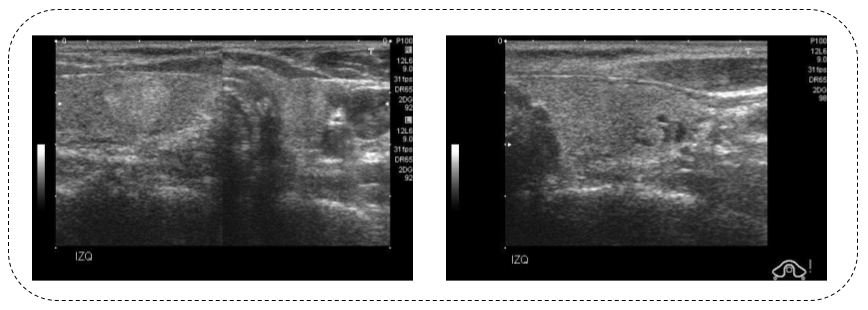
\includegraphics[width=0.85\textwidth]{4/figures/nodule_ddti.png}
		\caption[Ejemplo de imágenes del conjunto de datos de la Universidad de Colombia]{Ejemplo de imágenes del conjunto de datos de la Universidad de Colombia. \\
		Fuente: Elaboración propia.}
		\label{4:fig102}
	\end{center}
\end{figure}

\begin{figure}[H]
	\begin{center}
		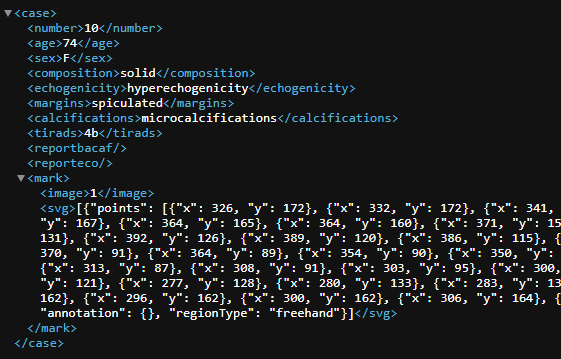
\includegraphics[width=0.65\textwidth]{4/figures/xmlfile.png}
		\caption[Ejemplo de archivo XML del conjunto de datos de la Universidad de Colombia]{Ejemplo de archivo XML del conjunto de datos de la Universidad de Colombia. \\
		Fuente: Elaboración propia.}
		\label{4:fig103}
	\end{center}
\end{figure}

Otro conjunto de datos, también de acceso libre, aunque no tan difundido como el presentado anteriormente es el otorgado por Zhujiang Hospital of Southem Medical University que recopila imágenes de 2421 pacientes obteniendo un total de 3493 imágenes de ultrasonido, de los cuales, 2283 pertenecen a imágenes de glándulas de tiroides con nódulos de carácter benigno, mientras que 1210 pertenecen a nódulos malignos. Además, este conjunto de datos también posee archivos CSV donde especifica el nombre de la imagen y la etiqueta a la que pertenece: benigno (0) o maligno (1).

Cabe destacar que este conjunto de datos posee características particulares que lo diferencian del primero, y es que este, además de estar validado por distintos comités de ética en China, procede de distintas fuentes; es decir, las imágenes pueden variar de tamaño y/o calidad entre sí.

En la Figura \ref{4:fig104} se muestran algunas imágenes de este conjunto de datos, mientras que en la Figura \ref{4:fig105} se muestra una sección de los archivos CSV.

\begin{figure}[H]
	\begin{center}
		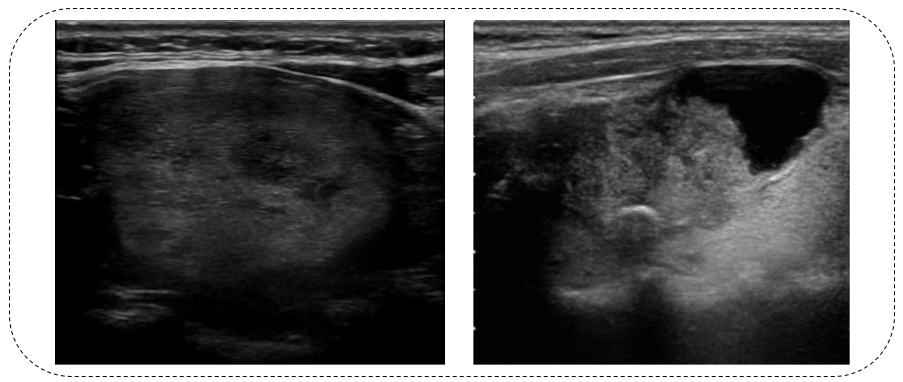
\includegraphics[width=0.68\textwidth]{4/figures/tn3k_examp.png}
		\caption[Ejemplo de imágenes del conjunto de datos de Zhujiang Hospital of Southem Medical University]{Ejemplo de imágenes del conjunto de datos de Zhujiang Hospital of Southem Medical University. \\
		Fuente: Elaboración propia.}
		\label{4:fig104}
	\end{center}
\end{figure}

\begin{figure}[H]
	\begin{center}
		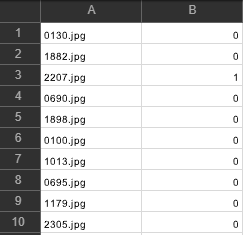
\includegraphics[width=0.38\textwidth]{4/figures/tn3k_csv.PNG}
		\caption[Ejemplo de archivo CSV del conjunto de datos de Zhujiang Hospital of Southem Medical University]{Ejemplo de archivo CSV del conjunto de datos de Zhujiang Hospital of Southem Medical University. \\
		Fuente: Elaboración propia.}
		\label{4:fig105}
	\end{center}
\end{figure}

\textbf{Actividad 2: Filtrado de los conjuntos de datos}
\\
Los requerimientos para un buen conjunto de datos radica principalmente en la información del tipo o carácter del nódulo, el origen de las imágenes de ultrasonido y la cantidad de datos.

El conjunto de datos otorgado por la Universidad de Colombia, CIM@LAB y IDIME poseía buena información, superando el requerimiento base de tipo o carácter del nódulo, pues otorgaba datos del paciente que podrían ser útiles a la hora de realizar el proceso de prediagnóstico; sin embargo, la gran debilidad del este conjunto de datos es la poca cantidad de imágenes que posee. Además, el hecho de no definirse el origen específico de estas imágenes en relación a si se obtuvo de distintas instituciones con diferentes herramientas o no, conllevó finalmente a su descarte.

El conjunto de datos de Zhujiang Hospital of Southem Medical University cumple exactamente con otorgar información sobre el carácter de los nódulos de cada imagen que posee, además, también se especifica el origen variado de las imágenes, pues fueron recopiladas de distintas instituciones y con diferentes herramientas. Finalmente, la cantidad de datos, aunque con clases desbalanceadas, supera en gran medida al primer conjunto de datos.

Al cumplir con todos los requerimientos para el entrenamiento de un buen modelo Deep Learning, el conjunto de datos finalmente seleccionado fue el de Zhujiang Hospital of Southem Medical University.

Como se mencionó en la sección anterior, la etapa siguiente es la de preprocesamiento. En este se realizó un completo análisis, limpieza y preparación de los datos para el entrenamiento de los modelos.

Cabe recordar además la existencia de dos flujos en este proceso igualmente descritos en la sección anterior. Ambos inician de igual forma con las tres siguientes actividades.

\textbf{Actividad 1: Explorar características del conjunto de datos}
\\
Ya con el conjunto de datos seleccionado, se utilizó la data almacenada en los archivos CSV (mostrado en la Figura \ref{4:fig105}) para contabilizar la cantidad de imágenes por cada clase y así determinar si existía o no la presencia de desbalance. La Figura \ref{4:fig106} y Figura \ref{4:fig107} muestran gráficas circulares donde se aprecia la proporción del total de datos por cada clase y por cada tipo de datos (entrenamiento y prueba).

\begin{figure}[H]
	\begin{center}
		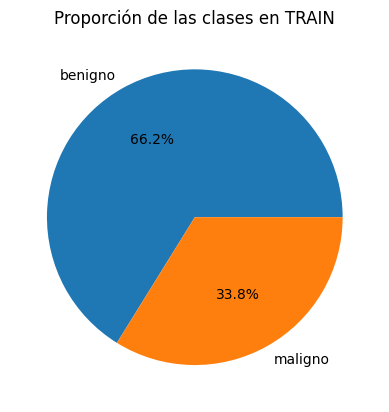
\includegraphics[width=0.51\textwidth]{4/figures/train_circular.png}
		\caption[Gráfica circular de conjunto de datos de entrenamiento]{Gráfica circular de conjunto de datos de entrenamiento. \\
		Fuente: Elaboración propia.}
		\label{4:fig106}
	\end{center}
\end{figure}

\begin{figure}[H]
	\begin{center}
		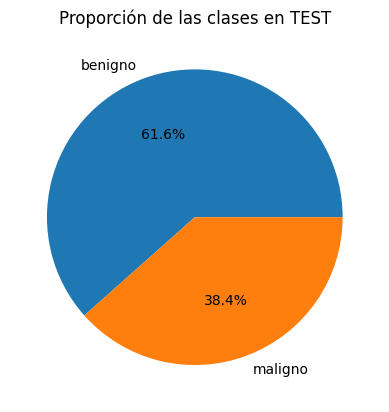
\includegraphics[width=0.51\textwidth]{4/figures/test_circular.png}
		\caption[Gráfica circular de conjunto de datos de prueba]{Gráfica circular de conjunto de datos de prueba. \\
		Fuente: Elaboración propia.}
		\label{4:fig107}
	\end{center}
\end{figure}

En ambas figuras se puede verificar la presencia de desbalance en clases, observando además como la clase de nódulos benignos duplica aproximadamente a la cantidad de imágenes de la clase de nódulos malignos. Este comportamiento se ve reflejado tanto para los datos de entrenamiento como para los de prueba.

Este descubrimiento afirmó la necesidad de aplicar una técnica de balanceo de datos.

\textbf{Actividad 2: Filtrar y organizar imágenes poco útiles del conjunto de datos}
\\
A través del Algoritmo \ref{4:alg101} se logró filtrar y obviar aquellas imágenes corruptas (en el caso de este conjunto de datos no se tuvo ninguno). Además, este también permitió la lectura de solo las imágenes con nombre presente en los archivos CSV, lo cual logró evitar el cargado de imágenes sin etiqueta alguna (en el caso de este conjunto de datos tampoco se tuvieron imágenes sin etiquetas). Finalmente, todas aquellos datos que cumplieran con los anteriores pasos serían trasladados a la nueva distribución de ficheros mostrada en la Figura \ref{4:fig109}.
%\hspace{\algorithmicindent} 
\begin{algorithm}[H]
	\caption{Proceso de organización y traslado de imágenes}
	\label{4:alg101}
	\begin{algorithmic}[1]
		\State \textbf{Entradas:} $pd\_train$, $pd\_test$, $source\_dir\_train$, $source\_dir\_test$, $train\_dir$, $test\_dir$
		\State Obtener nombres de imágenes de entrenamiento de $pd\_train$
		\State Crear diccionario $d$ de nombres a etiquetas de $pd\_train$
		\For{cada nombre de imagen $im$ en nombres de imágenes de entrenamiento}
			\State \textbf{Intentar:}
			\If{etiqueta de $im$ en $d$ es 1}
				\State Copiar $im$ a $train\_dir/malignant$
			\ElsIf{etiqueta de $im$ en $d$ es 0}
				\State Copiar $im$ a $train\_dir/benign$
			\EndIf
			\State \textbf{Excepción:}
			\State \textbf{Imprimir:} La imagen $im$ no se ha podido cargar...
		\EndFor

		\State Obtener nombres de imágenes de prueba de $pd\_test$
		\State Crear diccionario $dt$ de nombres a etiquetas de $pd\_test$
		\For{cada nombre de imagen $im$ en nombres de imágenes de prueba}
			\State \textbf{Intentar:}
			\If{etiqueta de $im$ en $dt$ es 1}
				\State Copiar $im$ a $test\_dir/malignant$
			\ElsIf{etiqueta de $im$ en $dt$ es 0}
				\State Copiar $im$ a $test\_dir/benign$
			\EndIf
			\State \textbf{Excepción:}
			\State \textbf{Imprimir:} La imagen $im$ no se ha podido cargar...
		\EndFor

		\State \textbf{Imprimir:} SE TRASLADARON TODAS LAS IMÁGENES AL NUEVO DIRECTORIO!
	\end{algorithmic}
\end{algorithm}

\begin{comment}
	\begin{figure}[H]
		\begin{center}
			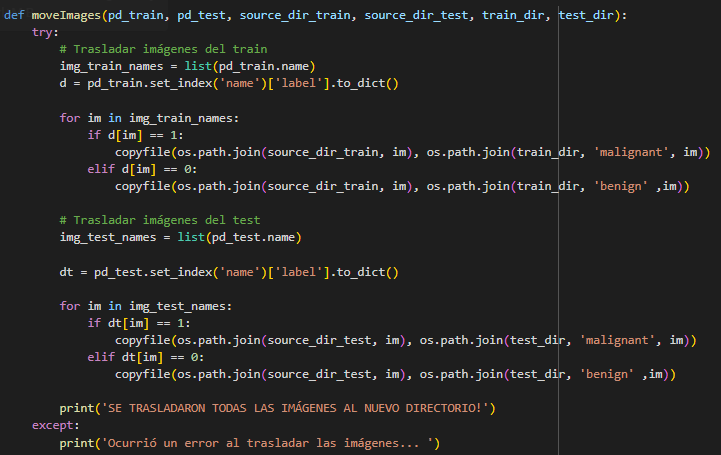
\includegraphics[width=0.75\textwidth]{4/figures/algoritm_organi.PNG}
			\caption[Algoritmo de organización de imágenes]{Algoritmo de organización de imágenes. \\
			Fuente: Elaboración propia.}
			\label{4:fig108}
		\end{center}
	\end{figure}
	


\begin{figure}[H]
	\begin{center}
		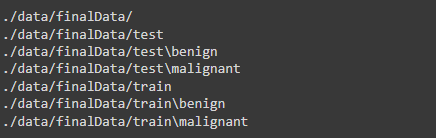
\includegraphics[width=0.60\textwidth]{4/figures/nuevos_ficheros.PNG}
		\caption[Nueva distribución de ficheros para los datos]{Nueva distribución de ficheros para los datos. \\
		Fuente: Elaboración propia.}
		\label{4:fig109}
	\end{center}
\end{figure}

\textbf{Actividad 3: Redimensionar, normalizar y dividir los datos según los requerimientos para cada modelo de Deep Learning}
\\
A partir de esta actividad, los datos usados fueron aquellos anteriormente trasladados desde los ficheros originales a los nuevos directorios.

El tamaño a redimensionar de las imágenes del conjunto de datos dependió únicamente del modelo en el que este se usó.

La normalización de los valores de píxeles de cada imagen se hizo con un media y desviación estándar de 0.5 aplicadas a cada uno de los 3 canales de las imágenes. Esto llevó a obtener finalmente píxeles con valores dentro del rango de [-1, 1], lo cual se recomienda para realizar entrenamientos de los modelos de forma más eficiente.

Finalmente, el conjunto de datos de entrenamiento se dividió en dos partes: data de validación, el cual representa el 15\% del total, y data de entrenamiento, compuesta del 85\% restante. La distribución de los datos se hizo de forma aleatoria manteniendo los mismos porcentajes.

La cantidad de la data de prueba se mantuvo igual a como originalmente fue obtenida.

Todo este proceso se realizó a través del Algoritmo \ref{4:alg102}, donde finalmente se otorgaron los tres conjuntos de datos en tipo DataLoader de Pytorch que posteriormente facilitó la ingesta de datos a los modelos.

\begin{algorithm}[H]
	\caption{Preparación de datos para entrenamiento, validación y prueba}
	\label{4:alg102}
	\begin{algorithmic}[1]
		\State \textbf{Entradas:} $train\_dir$, $test\_dir$, $img\_size$, $b\_size$
		\State \textbf{Salidas:} $train\_gen$, $val\_gen$, $test\_gen$
		
		\Procedure{DefinirTransformaciones}{}
			\State Redimensionar imágenes a $img\_size$
			\State Recortar las imágenes a $img\_size$
			\State Convertir imágenes a tensores
			\State Normalizar tensores con medias y desviaciones estándar $(0.5, 0.5, 0.5)$
		\EndProcedure
		
		\Procedure{CargarDatos}{}
			\State Cargar imágenes de entrenamiento de $train\_dir$ con transformaciones
			\State Cargar imágenes de prueba de $test\_dir$ con transformaciones
		\EndProcedure
		
		\Procedure{DividirDatosEntrenamiento}{}
			\State Calcular $val\_size$ como $15\%$ de $train\_data$
			\State Calcular $train\_size$ como $len(train\_data) - val\_size$
			\State Dividir de forma aleatoria $train\_data$ en $train\_data$ y $val\_data$ usando $train\_size$ y $val\_size$
		\EndProcedure
		
		\Procedure{CrearDataloaders}{}
			\State Crear $train\_gen$ para $train\_data$ con $b\_size$
			\State Crear $val\_gen$ para $val\_data$ con $b\_size$
			\State Crear $test\_gen$ para $test\_data$ con $b\_size$
		\EndProcedure
		
		\State \Return $train\_gen$, $val\_gen$, $test\_gen$
	\end{algorithmic}
\end{algorithm}

\begin{comment}
	\begin{figure}[H]
		\begin{center}
			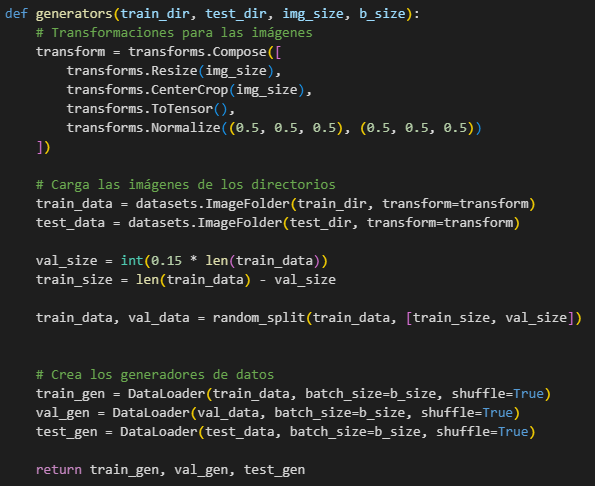
\includegraphics[width=0.70\textwidth]{4/figures/algoritm_dataloader.PNG}
			\caption[Algoritmo para lectura de los datos en DataLoader]{Algoritmo para lectura de los datos en DataLoader. \\
			Fuente: Elaboración propia.}
			\label{4:fig110}
		\end{center}
	\end{figure}


\textbf{Actividad 4: Mejorar composición del conjunto de datos}
\\
Como se ha mencionado en la sección anterior de este capítulo, las características que determinan si un nódulo puede ser benigno o maligno en un imagen de ultrasonido impiden el uso de las técnicas convencionales de Aumento de Datos. Por este motivo, se construyó un modelo DCGAN con el objetivo de generar imágenes sintéticas.

Inicialmente, la arquitectura del modelo DCGAN siguió los mismos lineamientos definidos en la página oficial de Pytorch por \cite{ws_inkawhich2024dcganpytorch}; sin embargo, debido a la posible pérdida de información al reducir considerablemente el tamaño de las imágenes (ya que se pedía como entrada imágenes de 64 x 64), se decidió por personalizar el modelo original para que pueda recibir imágenes de 128 x 128, de la misma manera como se hizo en la investigación presentada por \cite{pr_JERBI2023autoclassViTGAN}. Para lograr esto se tuvo que modificar tanto la red generadora como la discriminadora.

En la red generadora se agregaron un bloque nuevo de capas similar a las que ya poseída, modificando únicamente el tamaño de canales de salida de la capa ConvTranspose2d al doble de las que poseía la capa inicial original. El tamaño de kernel, stride y padding de esta misma capa se mantuvieron del formato original. En la capa de BatchNorm2d también se duplicó la cantidad de features que recibía. La función de activación ReLU se mantuvo con la misma configuración inicial. La capas siguientes a este nuevo bloque, fueron adaptándose a la cambiada cantidad de canales de salida.

El tamaño del vector latente que ingresa a la red generadora se definió en 200, con 3 como número de canales y 128 como cantidad base de features map.

En el caso de la red discriminadora, se introdujo un bloque intermedio de capas en la parte final de todo el grupo de bloque de capas similares. La capa Conv2d de este nuevo bloque recibiría la cantidad de canales de salida del bloque anterior, mientras que sus canales de salida serían el doble de los tenía la capa Conv2d anterior. De igual forma, la capa BatchNorm2d  duplicó la cantidad de features que recibía originalmente. Se mantuvo la misma configuración de la función de activación LeakyReLU. La capa siguiente a este bloque recién creado se modificó para recibir el doble de canales de los que recibía originalmente.

La cantidad de canales que recibía el modelo se estableció en 3, mientras que el número de features map base a generar se estableció a 32.

Todas las demás configuraciones en ambas redes se dejaron por defecto.

La Figura \ref{4:fig111} muestra la arquitectura final de la red generadora.

\begin{figure}[H]
	\begin{center}
		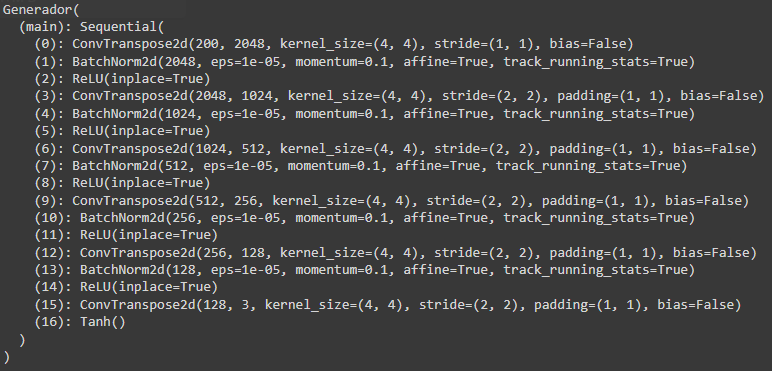
\includegraphics[width=0.78\textwidth]{4/figures/generator_network.PNG}
		\caption[Arquitectura de Red Generadora]{Arquitectura de Red Generadora. \\
		Fuente: Elaboración propia.}
		\label{4:fig111}
	\end{center}
\end{figure}

De igual forma, la Figura \ref{4:fig112}, muestra la arquitectura de la red discriminadora. 

\begin{figure}[H]
	\begin{center}
		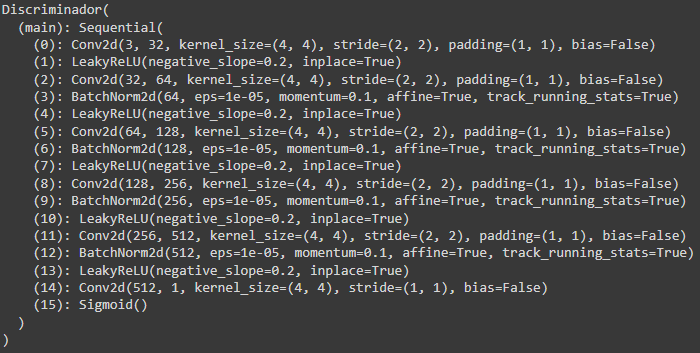
\includegraphics[width=0.76\textwidth]{4/figures/discriminator_network.PNG}
		\caption[Arquitectura de Red Discriminadora]{Arquitectura de Red Discriminadora. \\
		Fuente: Elaboración propia.}
		\label{4:fig112}
	\end{center}
\end{figure}

Para la función de pérdida se usó el Binary Cross Entropy Loss, mientras que la función de optimización se estableció en Adam con una tasa de aprendizaje de 0.0002 y betas de 0.5 para el primero y 0.999 para el segundo. Todo esto según lo establecido por la página oficial de Pytorch.

También se definió un tensor fijo de tamaño 200 (tamaño anteriormente definido de vector latente) inicializado con números aleatorios pero que siguen una distribución normal. Este tensor tenía un lote de tamaño 64.

Para ya iniciar con el entrenamiento del modelo DCGAN se procedió con la creación del DataLoader de Pytorch que contenía todas las imágenes del conjunto de datos de entrenamiento. En este proceso, se definió que las imágenes deberían ser redimensionadas a tamaño 128 y con leídas en un tamaño de lote 64.

El proceso de entrenamiento siguió las características normales del DCGAN original, estableciendo únicamente la cantidad de épocas a 200.

Se usó las capacidades de la GPU NVIDIA A100-SXM4-40GB obtenido a través de Google Colab para este proceso de entrenamiento.

En la Figura \ref{4:fig113} se muestran las métricas de la parte final del entrenamiento.

\begin{figure}[H]
	\begin{center}
		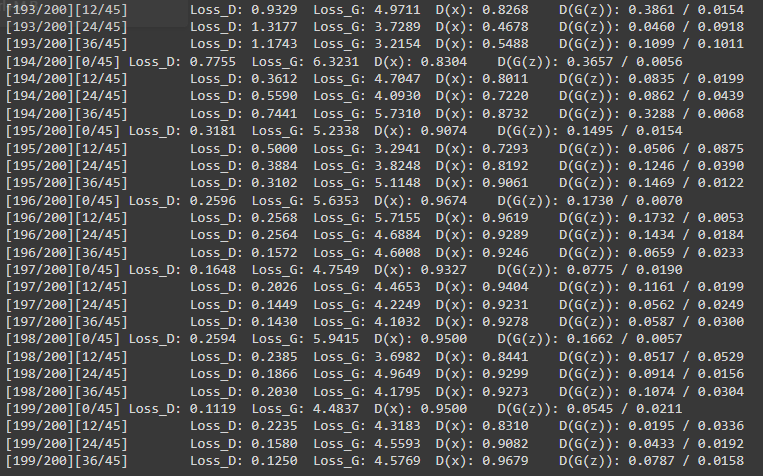
\includegraphics[width=0.75\textwidth]{4/figures/dcgan_1_train.PNG}
		\caption[Parte final del entrenamietno del DCGAN]{Parte final del entrenamietno del DCGAN. \\
		Fuente: Elaboración propia.}
		\label{4:fig113}
	\end{center}
\end{figure}

Además, se realizó un plot de las pérdidas de ambas redes a través de cada iteración del entrenamiento del modelo. Este se muestra en la Figura \ref{4:fig114}.

\begin{figure}[H]
	\begin{center}
		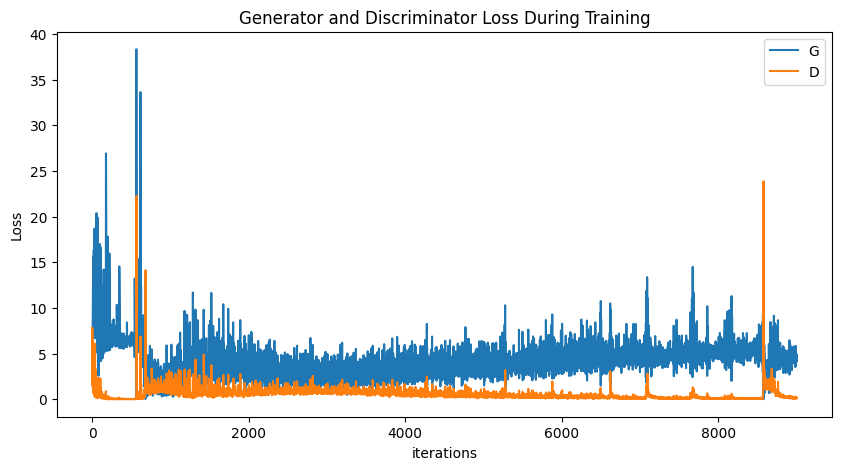
\includegraphics[width=0.85\textwidth]{4/figures/plot_loss_1.png}
		\caption[Plot de pérdidas de las red Generadora y Discriminadora]{Plot de pérdidas de las red Generadora y Discriminadora. \\
		Fuente: Elaboración propia.}
		\label{4:fig114}
	\end{center}
\end{figure}

En esta última gráfica se puede observar cómo ambas pérdidas van convergiendo a más iteraciones se tiene; sin embargo, ya en la parte final se logra observar la divergencia de ambos valores. Esto podría deberse a un sobreajuste por parte de la red discriminadora, al mismo tiempo que la red generadora deja de mejorar en la tarea de generar imágenes sintéticas.

Las imágenes reales y generadas se muestran en la Figura \ref{4:fig115}.

\begin{figure}[H]
	\begin{center}
		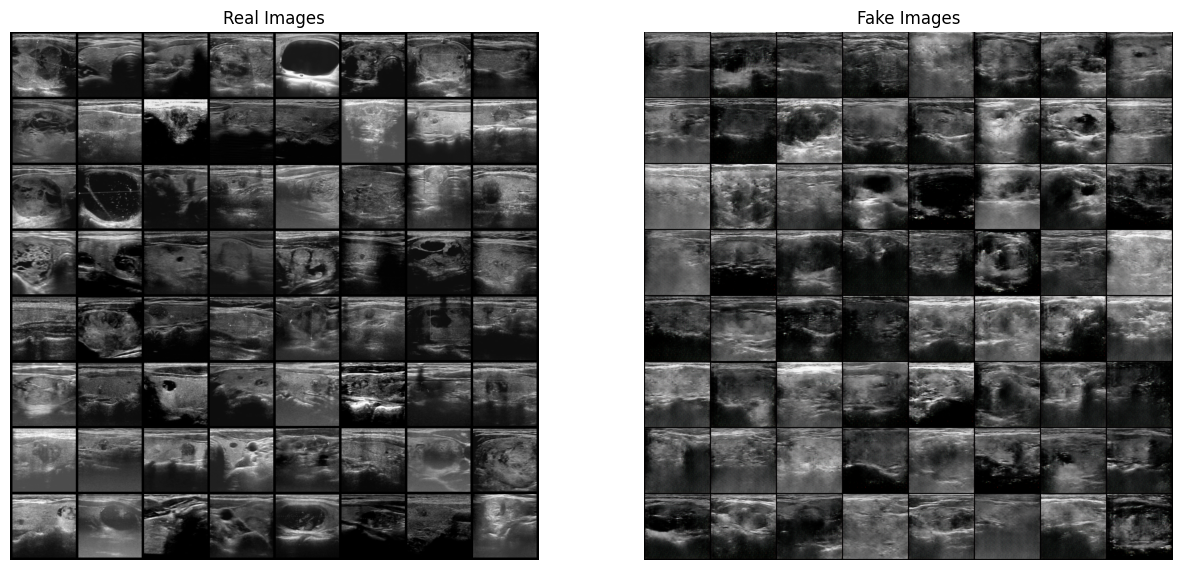
\includegraphics[width=0.85\textwidth]{4/figures/generated_real_1.png}
		\caption[Imágenes de ultrasonido de nódulos tiroideos generados y reales]{Imágenes de ultrasonido de nódulos tiroideos generados y reales. \\
		Fuente: Elaboración propia.}
		\label{4:fig115}
	\end{center}
\end{figure}

Según un rápido análisis visual, la imágenes generadas sí tienen un poco de similitud a las originales, y fácilmente, para alguien no experto, estos podrían pasar como imágenes reales.

Ya que el entrenamiento se realizó con todas las imágenes la data de entrenamiento, todas las imágenes generadas podrían pertenecer a cualquiera de las clases (benigno o maligno) y se es difícil sino imposible determinar a qué tipo pertenecen (benigno o maligno). Por este motivo, y viendo el potencial del DCGAN, se volvió a entrenar el modelo ahora solo con imágenes de la clase maligno (clase minoritaria) del conjunto de datos de entrenamiento para que la red solo pueda generar imágenes de ultrasonido de esta clase en específico.

En este caso se modificó el tamaño de vector latente a 300 y los features map base a 256 en la red generadora. Las demás configuraciones se mantuvieron, incluyendo aquellas de la red discriminadora.

Se usaron la misma función de pérdida y optimización con los mismos parámetros definidos anteriormente.

El tensor fijo de números aleatorio de distribución normal tuvo para este entrenamiento un tamaño de 300 (igual al tamaño del vector latente).

Para el DataLoader se mantuvo el mismo tamaño de redimensionamiento y lote.

Debido a una prueba rápida inicial con una menor cantidad de épocas, donde se obtuvieron pobres resultados, se decidió aumentar la cantidad de iteraciones totales estableciendo el número de épocas a 370.

La Figura \ref{4:fig116} muestra la parte final del entrenamiento.

\begin{figure}[H]
	\begin{center}
		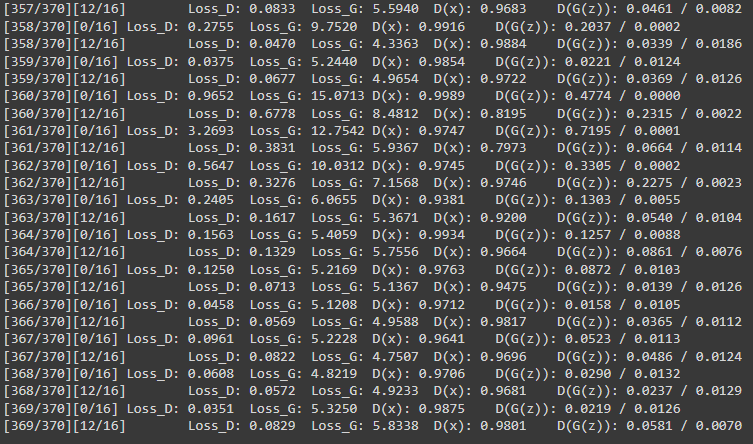
\includegraphics[width=0.75\textwidth]{4/figures/dcgan_2_train.PNG}
		\caption[Parte final del entrenamietno del DCGAN con imágenes de nódulos malignos]{Parte final del entrenamietno del DCGAN con imágenes de nódulos malignos. \\
		Fuente: Elaboración propia.}
		\label{4:fig116}
	\end{center}
\end{figure}

De igual manera al entrenamiento inicial, se realizó una gráfica donde se muestra el comportamiento de la pérdida en ambas redes. Esto se muestra en la Figura \ref{4:fig117}.

\begin{figure}[H]
	\begin{center}
		\includegraphics[width=0.85\textwidth]{4/figures/plot_loss_2.png}
		\caption[Plot de pérdidas de las red Generadora y Discriminadora de imágenes de nódulos malignos]{Plot de pérdidas de las red Generadora y Discriminadora de imágenes de nódulos malignos. \\
		Fuente: Elaboración propia.}
		\label{4:fig117}
	\end{center}
\end{figure}

Esta gráfica muestra el mismo comportamiento que a más iteraciones, mayor divergencia entre las pérdidas.

En la Figura \ref{4:fig118} se presentan las imágenes generadas junto a las originales.

\begin{figure}[H]
	\begin{center}
		\includegraphics[width=0.85\textwidth]{4/figures/generated_real_2.png}
		\caption[Imágenes de ultrasonido de nódulos tiroideos generados y reales (DCGAN de imágenes de nódulos malignos)]{Imágenes de ultrasonido de nódulos tiroideos generados y reales (DCGAN de imágenes de nódulos malignos). \\
		Fuente: Elaboración propia.}
		\label{4:fig118}
	\end{center}
\end{figure}

Los resultados de las imágenes generadas en este modelo muestran mayor ruido comparado las generadas con el entrenamiento inicial, esto se debe principalmente a la menor cantidad de datos usada para el entrenamiento de este nuevo DCGAN. Sin embargo, luego de un rápido análisis visual, se puede observar un comportamiento similar entre todas estas imágenes nuevas, y es que en la mayoría de estas hay lo que parece ser la presencia de un nódulo, aunque difuminado con mucho ruido aleatorio, esto podría indicar un aprendizaje cercano a la distribución de las imágenes de nódulos malignos.

Intentando utilizar el potencial que ofrece el DCGAN, se realizó posteriormente dos tipos de entrenamiento a los modelos de Deep Learning: el primero sin el Aumento de Datos a través de DCGAN, mientras que el segundo combinará los datos generados con la data original de entrenamiento para realizar dicho proceso. Esto permitirá determinar si las imágenes generadas por el DCGAN, aunque con ruido, son capaces de aumentar la capacidad de predicción de los modelos.

La gráfica circula presenta en la Figura \ref{4:fig119} muestra el nuevo balance entre ambas clases en la nueva data de entrenamiento.

\begin{figure}[H]
	\begin{center}
		\includegraphics[width=0.51\textwidth]{4/figures/balanced_circular.png}
		\caption[Gráfica circula de data de entrenamiento balanceada]{Gráfica circula de data de entrenamiento balanceada. \\
		Fuente: Elaboración propia.}
		\label{4:fig119}
	\end{center}
\end{figure}

Ya con la data preprocesada, se inició con la etapa de Aplicación de Deep Learning donde se entrenó, validó y puso a prueba los diversos modelos CNN y ViT. Esta etapa inicia con la siguiente actividad.

\textbf{Actividad 1: Seleccionar algoritmos a entrenar según usos y resultados de las investigaciones presentadas en los antecedentes}
\\
Según los datos analizados en las investigaciones presentadas en el Capítulo 2, el modelo con mayor presencia de los CNN es el ResNet50, mientras que por el lado de los modelos ViT, los más usados son los ViT-Base con tamaño de patch de 16 x 16.

Además, debido al tipo de problema de clasificación presente en esta investigación, y la similitud con el trabajo de \cite{pr_JERBI2023autoclassViTGAN}, se decidió por probar con las redes VGG16, ya que ha demostrado ser capaz de obtener un alto desempeño.

En resumen, se ha optado por utilizar las arquitecturas CNN de ResNet50 y VGG16. Además, como parte de las arquitecturas ViT, se optó por el uso de ViT-Base (16).

\textbf{Actividad 2: Entrenar y probar los modelos de Deep Learning previamente definidos}
\\
Para todas las arquitecturas de Deep Learning en esta investigación, se definió como función de activación el sigmoide. De igual manera, para el entrenamiento se usó la capacidad de la GPU NVIDIA A100-SXM4-40GB obtenido a través de Google Colab para lograr un rápido y eficiente entrenamiento. Además, se determinó una semilla de 2024 para permitir la reproducibilidad de los resultados. 

En este primer grupo, no se utilizará el conjunto de datos con imágenes generadas.

Se empezó con los modelos ViT-Base (16).

Para este proceso se crearon los DataLoader correspondientes con las características requeridas por estos modelos ViT: se redimensionaron las imágenes a 224 x 224 y se definió un tamaño de lote de 64 (este último tamaño será constante para todos los modelos mostrados en esta actividad).

En este primer modelo, se usó la técnica de entrenamiento de Fine Tuning junto con el modelo ViT-Base (16) con pesos de IMAGENET1KV1.

La función de pérdida aplicada fue el BCEWithLogitsLoss que evita el uso manual de la sigmoide y lo aplica directamente con la entropía cruzada. Nuevamente, esta función será utilizada en cada uno de los modelos en esta actividad.

Para lograr una clasificación binaria, las últimas capas de estas arquitecturas debió ser reemplazada por un MLP simple que recibe todos los features del modelo y produce una única salida. La configuración del MLP se definió de la forma (256, 1), donde el primer valor es el número de neuronas en la capas oculta que tuvo la función de activación ReLU, y el segundo valor es el número de neuronas en la capa de salida. Esta configuración de MLP se aplicó a todos los modelos ViT y CNN, a excepción de VGG16, donde se usó una configuración por defecto, únicamente modificando a 1 el número de neuronas en la capa de salida. En el caso de los modelos híbridos, solamente se etableció el bloque clasificador a una capa de salida con 1 neurona, debido a las limitaciones de disponibilidad de recursos computacionales.

Finalmente, la función de optimización utilizada fue Adam con una tasa de aprendizaje de 0.0001, y se definió para el entrenamiento 20 épocas. Las demás configuraciones se dejaron por defecto.

Estas configuraciones se aplicarán de igual manera a los demás modelos en esta actividad.

A continuación se presenta en la Figura \ref{4:fig120} el proceso de entrenamiento del modelo ViT-Base (16) con los pesos IMAGENET1KV1 y usando la técnica de Fine Tuning.

\begin{figure}[H]
	\begin{center}
		\includegraphics[width=0.85\textwidth]{4/figures/model1_train.PNG}
		\caption[Proceso de entrenamiento del modelo n°1]{Proceso de entrenamiento del modelo n°1. \\
		Fuente: Elaboración propia.}
		\label{4:fig120}
	\end{center}
\end{figure}

Finalmente, para este modelo también se calcularon su Accuracy, Recall y Precision. Estos son presentados en la Tabla \ref{4:table2}.

\begin{table}[H]
	\caption[Accuracy, Recall y Precision del modelo n°1]{Accuracy, Recall y Precision del modelo n°1.}
	\label{4:table2}
	\centering
	\small
	\begin{tabular}{c|ccc}
		\specialrule{.1em}{.05em}{.05em}
		{Métrica} & {Accuracy} & {Recall} & {Precision} \\
		\hline
		{Valor} & {69.54\%} & {47.03\%} & {64.16\%} \\
		\specialrule{.1em}{.05em}{.05em}
	\end{tabular}
	\begin{flushleft}	
		\small Fuente: Elaboración propia.
	\end{flushleft}
\end{table}

\begin{comment}
\begin{figure}[H]
	\begin{center}
		\includegraphics[width=0.83\textwidth]{4/figures/model1_rp.PNG}
		\caption[Accuracy, Recall y Precision del modelo n°1]{Recall y Precision del modelo n°1. \\
		Fuente: Elaboración propia.}
		\label{4:fig121}
	\end{center}
\end{figure}


En el siguiente modelo, se usó la técnica de entrenamiento de Transfer Learning junto con el modelo ViT-Base (16) con pesos de IMAGENET1KV1.

El DataLoader constaba de las imágenes redimensionadas nuevamente a 224 x 224, y se aplicó la función de pérdida BCEWithLogitsLoss junto con la función de optimización Adam.

A continuación se presenta en la Figura \ref{4:fig122} el proceso de entrenamiento del modelo ViT-Base (16) con los pesos IMAGENET1KV1 y usando la técnica de Transfer Learning.

\begin{figure}[H]
	\begin{center}
		\includegraphics[width=0.85\textwidth]{4/figures/model2_train.PNG}
		\caption[Proceso de entrenamiento del modelo n°2]{Proceso de entrenamiento del modelo n°2. \\
		Fuente: Elaboración propia.}
		\label{4:fig122}
	\end{center}
\end{figure}

También se calcularon su Accuracy, Recall y Precision. Estos son presentados en la Tabla \ref{4:table3}.

\begin{table}[H]
	\caption[Accuracy, Recall y Precision del modelo n°2]{Accuracy, Recall y Precision del modelo n°2.}
	\label{4:table3}
	\centering
	\small
	\begin{tabular}{c|ccc}
		\specialrule{.1em}{.05em}{.05em}
		{Métrica} & {Accuracy} & {Recall} & {Precision} \\
		\hline
		{Valor} & {68.08\%} & {53.39\%} & {59.43\%} \\
		\specialrule{.1em}{.05em}{.05em}
	\end{tabular}
	\begin{flushleft}	
		\small Fuente: Elaboración propia.
	\end{flushleft}
\end{table}

\begin{comment}
\begin{figure}[H]
	\begin{center}
		\includegraphics[width=0.83\textwidth]{4/figures/model2_rp.PNG}
		\caption[Recall y Precision del modelo n°2]{Recall y Precision del modelo n°2. \\
		Fuente: Elaboración propia.}
		\label{4:fig123}
	\end{center}
\end{figure}


Este modelo usó la técnica de entrenamiento de Fine Tuning junto con el modelo ViT-Base (16) con pesos de IMAGENET1KSWAGE2EV1.

En este caso, el DataLoader constaba de las imágenes redimensionadas a 384 x 384.

Se presenta en la Figura \ref{4:fig124} el proceso de entrenamiento del modelo ViT-Base (16) con los pesos  IMAGENET1KSWAGE2EV1 y usando la técnica de Fine Tuning.

\begin{figure}[H]
	\begin{center}
		\includegraphics[width=0.85\textwidth]{4/figures/model3_train.PNG}
		\caption[Proceso de entrenamiento del modelo n°3]{Proceso de entrenamiento del modelo n°3. \\
		Fuente: Elaboración propia.}
		\label{4:fig124}
	\end{center}
\end{figure}

También se calcularon su Accuracy, Recall y Precision. Estos son presentados en la Tabla \ref{4:table4}.

\begin{table}[H]
	\caption[Accuracy, Recall y Precision del modelo n°3]{Accuracy, Recall y Precision del modelo n°3.}
	\label{4:table4}
	\centering
	\small
	\begin{tabular}{c|ccc}
		\specialrule{.1em}{.05em}{.05em}
		{Métrica} & {Accuracy} & {Recall} & {Precision} \\
		\hline
		{Valor} & {56.84\%} & {53.81\%} & {44.88\%} \\
		\specialrule{.1em}{.05em}{.05em}
	\end{tabular}
	\begin{flushleft}	
		\small Fuente: Elaboración propia.
	\end{flushleft}
\end{table}

\begin{comment}
\begin{figure}[H]
	\begin{center}
		\includegraphics[width=0.83\textwidth]{4/figures/model3_rp.PNG}
		\caption[Recall y Precision del modelo n°3]{Recall y Precision del modelo n°3. \\
		Fuente: Elaboración propia.}
		\label{4:fig125}
	\end{center}
\end{figure}

El modelo n°4 empleó la técnica de entrenamiento de Transfer Learning junto con el modelo ViT-Base (16) con pesos de IMAGENET1KSWAGE2EV1.

En este caso, nuevamente el DataLoader constaba de las imágenes redimensionadas a 384 x 384.

Se presenta en la Figura \ref{4:fig126} el proceso de entrenamiento del modelo ViT-Base (16) con los pesos IMAGENET1KSWAGE2EV1 y usando la técnica de Transfer Learning.

\begin{figure}[H]
	\begin{center}
		\includegraphics[width=0.85\textwidth]{4/figures/model4_train.PNG}
		\caption[Proceso de entrenamiento del modelo n°4]{Proceso de entrenamiento del modelo n°4. \\
		Fuente: Elaboración propia.}
		\label{4:fig126}
	\end{center}
\end{figure}

También se calcularon su Accuracy, Recall y Precision. Estos son presentados en la Tabla \ref{4:table5}.

\begin{table}[H]
	\caption[Accuracy, Recall y Precision del modelo n°4]{Accuracy, Recall y Precision del modelo n°4.}
	\label{4:table5}
	\centering
	\small
	\begin{tabular}{c|ccc}
		\specialrule{.1em}{.05em}{.05em}
		{Métrica} & {Accuracy} & {Recall} & {Precision} \\
		\hline
		{Valor} & {69.22\%} & {55.51\%} & {60.93\%} \\
		\specialrule{.1em}{.05em}{.05em}
	\end{tabular}
	\begin{flushleft}	
		\small Fuente: Elaboración propia.
	\end{flushleft}
\end{table}


\begin{figure}[H]
	\begin{center}
		\includegraphics[width=0.83\textwidth]{4/figures/model4_rp.PNG}
		\caption[Recall y Precision del modelo n°4]{Recall y Precision del modelo n°4. \\
		Fuente: Elaboración propia.}
		\label{4:fig127}
	\end{center}
\end{figure}


El modelo n°5 empleó la técnica de entrenamiento de Fine Tuning junto con el modelo ViT-Base (16) con pesos de IMAGENET1KSWAGLINEARV1.

En este caso, el DataLoader constaba de las imágenes redimensionadas a 224 x 224.

Se presenta en la Figura \ref{4:fig128} el proceso de entrenamiento del modelo ViT-Base (16) con los pesos IMAGENET1KSWAGLINEARV1 y usando la técnica de Fine Tuning.

\begin{figure}[H]
	\begin{center}
		\includegraphics[width=0.85\textwidth]{4/figures/model5_train.PNG}
		\caption[Proceso de entrenamiento del modelo n°5]{Proceso de entrenamiento del modelo n°5. \\
		Fuente: Elaboración propia.}
		\label{4:fig128}
	\end{center}
\end{figure}

También se calcularon su Recall y Precision. Estos son presentados en la Tabla \ref{4:table6}.

\begin{table}[H]
	\caption[Accuracy, Recall y Precision del modelo n°5]{Accuracy, Recall y Precision del modelo n°5.}
	\label{4:table6}
	\centering
	\small
	\begin{tabular}{c|ccc}
		\specialrule{.1em}{.05em}{.05em}
		{Métrica} & {Accuracy} & {Recall} & {Precision} \\
		\hline
		{Valor} & {58.47\%} & {34.75\%} & {44.81\%} \\
		\specialrule{.1em}{.05em}{.05em}
	\end{tabular}
	\begin{flushleft}	
		\small Fuente: Elaboración propia.
	\end{flushleft}
\end{table}

\begin{comment}
\begin{figure}[H]
	\begin{center}
		\includegraphics[width=0.83\textwidth]{4/figures/model5_rp.PNG}
		\caption[Recall y Precision del modelo n°5]{Recall y Precision del modelo n°5. \\
		Fuente: Elaboración propia.}
		\label{4:fig129}
	\end{center}
\end{figure}

El modelo n°6 empleó la técnica de entrenamiento de Transfer Learning junto con el modelo ViT-Base (16) con pesos de IMAGENET1KSWAGLINEARV1.

En este caso, el DataLoader constaba nuevamente de las imágenes redimensionadas a 224 x 224.

Se presenta en la Figura \ref{4:fig130} el proceso de entrenamiento del modelo ViT-Base (16) con los pesos IMAGENET1KSWAGLINEARV1 y usando la técnica de Transfer Learning.

\begin{figure}[H]
	\begin{center}
		\includegraphics[width=0.85\textwidth]{4/figures/model6_train.PNG}
		\caption[Proceso de entrenamiento del modelo n°6]{Proceso de entrenamiento del modelo n°6. \\
		Fuente: Elaboración propia.}
		\label{4:fig130}
	\end{center}
\end{figure}

También se calcularon su Accuracy, Recall y Precision. Estos son presentados en la Tabla \ref{4:table7}.

\begin{table}[H]
	\caption[Accuracy, Recall y Precision del modelo n°6]{Accuracy, Recall y Precision del modelo n°6.}
	\label{4:table7}
	\centering
	\small
	\begin{tabular}{c|ccc}
		\specialrule{.1em}{.05em}{.05em}
		{Métrica} & {Accuracy} & {Recall} & {Precision} \\
		\hline
		{Valor} & {65.31\%} & {41.95\%} & {56.57\%} \\
		\specialrule{.1em}{.05em}{.05em}
	\end{tabular}
	\begin{flushleft}	
		\small Fuente: Elaboración propia.
	\end{flushleft}
\end{table}

\begin{comment}
\begin{figure}[H]
	\begin{center}
		\includegraphics[width=0.83\textwidth]{4/figures/model6_rp.PNG}
		\caption[Recall y Precision del modelo n°6]{Recall y Precision del modelo n°6. \\
		Fuente: Elaboración propia.}
		\label{4:fig131}
	\end{center}
\end{figure}

El modelo n°7 empleó la técnica de entrenamiento de Fine Tuning junto con el modelo VGG16 con pesos de IMAGENET1KV1.

En este caso, el DataLoader fue cargado con imágenes redimensionadas a 128 x 128. Este tamaño será constante para los demás modelos CNN.

Se presenta en la Figura \ref{4:fig132} el proceso de entrenamiento del modelo VGG16 con los pesos IMAGENET1KV1 y usando la técnica de Fine Tuning.

\begin{figure}[H]
	\begin{center}
		\includegraphics[width=0.85\textwidth]{4/figures/model7_train.PNG}
		\caption[Proceso de entrenamiento del modelo n°7]{Proceso de entrenamiento del modelo n°7. \\
		Fuente: Elaboración propia.}
		\label{4:fig132}
	\end{center}
\end{figure}

También se calcularon su Accuracy, Recall y Precision. Estos son presentados en la Tabla \ref{4:table8}.

\begin{table}[H]
	\caption[Accuracy, Recall y Precision del modelo n°7]{Accuracy, Recall y Precision del modelo n°7.}
	\label{4:table8}
	\centering
	\small
	\begin{tabular}{c|ccc}
		\specialrule{.1em}{.05em}{.05em}
		{Métrica} & {Accuracy} & {Recall} & {Precision} \\
		\hline
		{Valor} & {71.99\%} & {58.90\%} & {64.95\%} \\
		\specialrule{.1em}{.05em}{.05em}
	\end{tabular}
	\begin{flushleft}	
		\small Fuente: Elaboración propia.
	\end{flushleft}
\end{table}

\begin{comment}
\begin{figure}[H]
	\begin{center}
		\includegraphics[width=0.83\textwidth]{4/figures/model7_rp.PNG}
		\caption[Recall y Precision del modelo n°7]{Recall y Precision del modelo n°7. \\
		Fuente: Elaboración propia.}
		\label{4:fig133}
	\end{center}
\end{figure}

El modelo n°8 empleó la técnica de entrenamiento de Transfer Learning junto con el modelo VGG16 con pesos de IMAGENET1KV1.

Se presenta en la Figura \ref{4:fig134} el proceso del entrenamiento del modelo VGG16 con los pesos IMAGENET1KV1 y usando la técnica de Transfer Learning.

\begin{figure}[H]
	\begin{center}
		\includegraphics[width=0.85\textwidth]{4/figures/model8_train.PNG}
		\caption[Proceso de entrenamiento del modelo n°8]{Proceso de entrenamiento del modelo n°8. \\
		Fuente: Elaboración propia.}
		\label{4:fig134}
	\end{center}
\end{figure}

También se calcularon su Accuracy, Recall y Precision. Estos son presentados en la Tabla \ref{4:table9}.

\begin{table}[H]
	\caption[Accuracy, Recall y Precision del modelo n°8]{Accuracy, Recall y Precision del modelo n°8.}
	\label{4:table9}
	\centering
	\small
	\begin{tabular}{c|ccc}
		\specialrule{.1em}{.05em}{.05em}
		{Métrica} & {Accuracy} & {Recall} & {Precision} \\
		\hline
		{Valor} & {65.80\%} & {67.37\%} & {54.45\%} \\
		\specialrule{.1em}{.05em}{.05em}
	\end{tabular}
	\begin{flushleft}	
		\small Fuente: Elaboración propia.
	\end{flushleft}
\end{table}

\begin{comment}
\begin{figure}[H]
	\begin{center}
		\includegraphics[width=0.83\textwidth]{4/figures/model8_rp.PNG}
		\caption[Recall y Precision del modelo n°8]{Recall y Precision del modelo n°8. \\
		Fuente: Elaboración propia.}
		\label{4:fig135}
	\end{center}
\end{figure}

El modelo n°9 empleó la técnica de entrenamiento de Fine Tuning junto con el modelo RESNET50 con pesos de IMAGENET1KV1.

Se presenta en la Figura \ref{4:fig136} el proceso del entrenamiento del modelo RESNET50 con los pesos IMAGENET1KV1 y usando la técnica de Fine Tuning.

\begin{figure}[H]
	\begin{center}
		\includegraphics[width=0.85\textwidth]{4/figures/model9_train.PNG}
		\caption[Proceso de entrenamiento del modelo n°9]{Proceso de entrenamiento del modelo n°9. \\
		Fuente: Elaboración propia.}
		\label{4:fig136}
	\end{center}
\end{figure}

También se calcularon su Accuracy, Recall y Precision. Estos son presentados en la Tabla \ref{4:table10}.

\begin{table}[H]
	\caption[Accuracy, Recall y Precision del modelo n°9]{Accuracy, Recall y Precision del modelo n°9.}
	\label{4:table10}
	\centering
	\small
	\begin{tabular}{c|ccc}
		\specialrule{.1em}{.05em}{.05em}
		{Métrica} & {Accuracy} & {Recall} & {Precision} \\
		\hline
		{Valor} & {72.48\%} & {58.90\%} & {65.88\%} \\
		\specialrule{.1em}{.05em}{.05em}
	\end{tabular}
	\begin{flushleft}	
		\small Fuente: Elaboración propia.
	\end{flushleft}
\end{table}

\begin{comment}
\begin{figure}[H]
	\begin{center}
		\includegraphics[width=0.83\textwidth]{4/figures/model9_rp.PNG}
		\caption[Recall y Precision del modelo n°9]{Recall y Precision del modelo n°9. \\
		Fuente: Elaboración propia.}
		\label{4:fig137}
	\end{center}
\end{figure}

El modelo n°10 empleó la técnica de entrenamiento de Transfer Learning  junto con el modelo RESNET50 con pesos de IMAGENET1KV1.

Se presenta en la Figura \ref{4:fig138} el proceso del entrenamiento del modelo RESNET50 con los pesos IMAGENET1KV1 y usando la técnica de Transfer Learning.

\begin{figure}[H]
	\begin{center}
		\includegraphics[width=0.85\textwidth]{4/figures/model10_train.PNG}
		\caption[Proceso de entrenamiento del modelo n°10]{Proceso de entrenamiento del modelo n°10. \\
		Fuente: Elaboración propia.}
		\label{4:fig138}
	\end{center}
\end{figure}

También se calcularon su Accuracy, Recall y Precision. Estos son presentados en la Tabla \ref{4:table11}.

\begin{table}[H]
	\caption[Accuracy, Recall y Precision del modelo n°10]{Accuracy, Recall y Precision del modelo n°10.}
	\label{4:table11}
	\centering
	\small
	\begin{tabular}{c|ccc}
		\specialrule{.1em}{.05em}{.05em}
		{Métrica} & {Accuracy} & {Recall} & {Precision} \\
		\hline
		{Valor} & {62.38\%} & {37.71\%} & {51.45\%} \\
		\specialrule{.1em}{.05em}{.05em}
	\end{tabular}
	\begin{flushleft}	
		\small Fuente: Elaboración propia.
	\end{flushleft}
\end{table}

\begin{comment}
\begin{figure}[H]
	\begin{center}
		\includegraphics[width=0.83\textwidth]{4/figures/model10_rp.PNG}
		\caption[Recall y Precision del modelo n°10]{Recall y Precision del modelo n°10. \\
		Fuente: Elaboración propia.}
		\label{4:fig139}
	\end{center}
\end{figure}

El modelo n°11 empleó la técnica de entrenamiento de Fine Tuning junto con el modelo RESNET50 con pesos de IMAGENET1KV2.

Se presenta en la Figura \ref{4:fig140} el proceso del entrenamiento del modelo RESNET50 con los pesos IMAGENET1KV2 y usando la técnica de Fine Tuning.

\begin{figure}[H]
	\begin{center}
		\includegraphics[width=0.85\textwidth]{4/figures/model11_train.PNG}
		\caption[Proceso de entrenamiento del modelo n°11]{Proceso de entrenamiento del modelo n°11. \\
		Fuente: Elaboración propia.}
		\label{4:fig140}
	\end{center}
\end{figure}

También se calcularon su Accuracy, Recall y Precision. Estos son presentados en la Tabla \ref{4:table12}.

\begin{table}[H]
	\caption[Accuracy, Recall y Precision del modelo n°11]{Accuracy, Recall y Precision del modelo n°11.}
	\label{4:table12}
	\centering
	\small
	\begin{tabular}{c|ccc}
		\specialrule{.1em}{.05em}{.05em}
		{Métrica} & {Accuracy} & {Recall} & {Precision} \\
		\hline
		{Valor} & {67.59\%} & {51.27\%} & {59.02\%} \\
		\specialrule{.1em}{.05em}{.05em}
	\end{tabular}
	\begin{flushleft}	
		\small Fuente: Elaboración propia.
	\end{flushleft}
\end{table}

\begin{comment}
\begin{figure}[H]
	\begin{center}
		\includegraphics[width=0.83\textwidth]{4/figures/model11_rp.PNG}
		\caption[Recall y Precision del modelo n°11]{Recall y Precision del modelo n°11. \\
		Fuente: Elaboración propia.}
		\label{4:fig141}
	\end{center}
\end{figure}

El modelo n°12 empleó la técnica de entrenamiento de Transfer Learning junto con el modelo RESNET50 con pesos de IMAGENET1KV2.

Se presenta en la Figura \ref{4:fig142} el proceso del entrenamiento del modelo RESNET50 con los pesos IMAGENET1KV2 y usando la técnica de Transfer Learning.

\begin{figure}[H]
	\begin{center}
		\includegraphics[width=0.85\textwidth]{4/figures/model12_train.PNG}
		\caption[Proceso de entrenamiento del modelo n°12]{Proceso de entrenamiento del modelo n°12. \\
		Fuente: Elaboración propia.}
		\label{4:fig142}
	\end{center}
\end{figure}

También se calcularon su Accuracy, Recall y Precision. Estos son presentados en la Tabla \ref{4:table13}.

\begin{table}[H]
	\caption[Accuracy, Recall y Precision del modelo n°12]{Accuracy, Recall y Precision del modelo n°12.}
	\label{4:table13}
	\centering
	\small
	\begin{tabular}{c|ccc}
		\specialrule{.1em}{.05em}{.05em}
		{Métrica} & {Accuracy} & {Recall} & {Precision} \\
		\hline
		{Valor} & {62.05\%} & {49.15\%} & {50.66\%} \\
		\specialrule{.1em}{.05em}{.05em}
	\end{tabular}
	\begin{flushleft}	
		\small Fuente: Elaboración propia.
	\end{flushleft}
\end{table}

\begin{comment}
\begin{figure}[H]
	\begin{center}
		\includegraphics[width=0.83\textwidth]{4/figures/model12_rp.PNG}
		\caption[Recall y Precision del modelo n°12]{Recall y Precision del modelo n°12. \\
		Fuente: Elaboración propia.}
		\label{4:fig143}
	\end{center}
\end{figure}

Una vez culminado el entrenamiento de los modelos con el conjunto de datos sin imágenes generadas, se inició un nuevo proceso de entrenamiento, esta vez con el conjunto de datos aumentado. 

Todos los modelos, tanto ViT como CNN, poseen las mismas configuraciones definidas antes, así que no hay necesidad de especificarlo nuevamente.

A continuación se presentan las siguientes Figuras y Tablas donde se muestran todos los resultados de los modelos de manera similar a como se presentó anteriormente.

\begin{figure}[H]
	\begin{center}
		\includegraphics[width=0.85\textwidth]{4/figures/model13_train.PNG}
		\caption[Proceso de entrenamiento del modelo n°13]{Proceso de entrenamiento del modelo n°13. \\
		Fuente: Elaboración propia.}
		\label{4:fig144}
	\end{center}
\end{figure}

\begin{table}[H]
	\caption[Accuracy, Recall y Precision del modelo n°13]{Accuracy, Recall y Precision del modelo n°13.}
	\label{4:table14}
	\centering
	\small
	\begin{tabular}{c|ccc}
		\specialrule{.1em}{.05em}{.05em}
		{Métrica} & {Accuracy} & {Recall} & {Precision} \\
		\hline
		{Valor} & {70.36\%} & {61.44\%} & {61.44\%} \\
		\specialrule{.1em}{.05em}{.05em}
	\end{tabular}
	\begin{flushleft}	
		\small Fuente: Elaboración propia.
	\end{flushleft}
\end{table}

\begin{comment}
\begin{figure}[H]
	\begin{center}
		\includegraphics[width=0.83\textwidth]{4/figures/model13_rp.PNG}
		\caption[Recall y Precision del modelo n°13]{Recall y Precision del modelo n°13. \\
		Fuente: Elaboración propia.}
		\label{4:fig145}
	\end{center}
\end{figure}

\begin{figure}[H]
	\begin{center}
		\includegraphics[width=0.85\textwidth]{4/figures/model14_train.PNG}
		\caption[Proceso de entrenamiento del modelo n°14]{Proceso de entrenamiento del modelo n°14. \\
		Fuente: Elaboración propia.}
		\label{4:fig146}
	\end{center}
\end{figure}

\begin{table}[H]
	\caption[Accuracy, Recall y Precision del modelo n°14]{Accuracy, Recall y Precision del modelo n°14.}
	\label{4:table15}
	\centering
	\small
	\begin{tabular}{c|ccc}
		\specialrule{.1em}{.05em}{.05em}
		{Métrica} & {Accuracy} & {Recall} & {Precision} \\
		\hline
		{Valor} & {69.06\%} & {50.00\%} & {62.11\%} \\
		\specialrule{.1em}{.05em}{.05em}
	\end{tabular}
	\begin{flushleft}	
		\small Fuente: Elaboración propia.
	\end{flushleft}
\end{table}

\begin{comment}
\begin{figure}[H]
	\begin{center}
		\includegraphics[width=0.83\textwidth]{4/figures/model14_rp.PNG}
		\caption[Recall y Precision del modelo n°14]{Recall y Precision del modelo n°14. \\
		Fuente: Elaboración propia.}
		\label{4:fig147}
	\end{center}
\end{figure}

\begin{figure}[H]
	\begin{center}
		\includegraphics[width=0.85\textwidth]{4/figures/model15_train.PNG}
		\caption[Proceso de entrenamiento del modelo n°15]{Proceso de entrenamiento del modelo n°15. \\
		Fuente: Elaboración propia.}
		\label{4:fig148}
	\end{center}
\end{figure}

\begin{table}[H]
	\caption[Accuracy, Recall y Precision del modelo n°15]{Accuracy, Recall y Precision del modelo n°15.}
	\label{4:table16}
	\centering
	\small
	\begin{tabular}{c|ccc}
		\specialrule{.1em}{.05em}{.05em}
		{Métrica} & {Accuracy} & {Recall} & {Precision} \\
		\hline
		{Valor} & {67.43\%} & {41.10\%} & {61.39\%} \\
		\specialrule{.1em}{.05em}{.05em}
	\end{tabular}
	\begin{flushleft}	
		\small Fuente: Elaboración propia.
	\end{flushleft}
\end{table}

\begin{comment}
\begin{figure}[H]
	\begin{center}
		\includegraphics[width=0.83\textwidth]{4/figures/model15_rp.PNG}
		\caption[Recall y Precision del modelo n°15]{Recall y Precision del modelo n°15. \\
		Fuente: Elaboración propia.}
		\label{4:fig149}
	\end{center}
\end{figure}

\begin{figure}[H]
	\begin{center}
		\includegraphics[width=0.85\textwidth]{4/figures/model16_train.PNG}
		\caption[Proceso de entrenamiento del modelo n°16]{Proceso de entrenamiento del modelo n°16. \\
		Fuente: Elaboración propia.}
		\label{4:fig150}
	\end{center}
\end{figure}

\begin{table}[H]
	\caption[Accuracy, Recall y Precision del modelo n°16]{Accuracy, Recall y Precision del modelo n°16.}
	\label{4:table17}
	\centering
	\small
	\begin{tabular}{c|ccc}
		\specialrule{.1em}{.05em}{.05em}
		{Métrica} & {Accuracy} & {Recall} & {Precision} \\
		\hline
		{Valor} & {69.71\%} & {64.83\%} & {59.77\%} \\
		\specialrule{.1em}{.05em}{.05em}
	\end{tabular}
	\begin{flushleft}	
		\small Fuente: Elaboración propia.
	\end{flushleft}
\end{table}

\begin{comment}
\begin{figure}[H]
	\begin{center}
		\includegraphics[width=0.83\textwidth]{4/figures/model16_rp.PNG}
		\caption[Recall y Precision del modelo n°16]{Recall y Precision del modelo n°16. \\
		Fuente: Elaboración propia.}
		\label{4:fig151}
	\end{center}
\end{figure}

\begin{figure}[H]
	\begin{center}
		\includegraphics[width=0.85\textwidth]{4/figures/model17_train.PNG}
		\caption[Proceso de entrenamiento del modelo n°17]{Proceso de entrenamiento del modelo n°17. \\
		Fuente: Elaboración propia.}
		\label{4:fig152}
	\end{center}
\end{figure}

\begin{table}[H]
	\caption[Accuracy, Recall y Precision del modelo n°17]{Accuracy, Recall y Precision del modelo n°17.}
	\label{4:table18}
	\centering
	\small
	\begin{tabular}{c|ccc}
		\specialrule{.1em}{.05em}{.05em}
		{Métrica} & {Accuracy} & {Recall} & {Precision} \\
		\hline
		{Valor} & {57.65\%} & {41.95\%} & {44.59\%} \\
		\specialrule{.1em}{.05em}{.05em}
	\end{tabular}
	\begin{flushleft}	
		\small Fuente: Elaboración propia.
	\end{flushleft}
\end{table}

\begin{comment}
\begin{figure}[H]
	\begin{center}
		\includegraphics[width=0.83\textwidth]{4/figures/model17_rp.PNG}
		\caption[Recall y Precision del modelo n°17]{Recall y Precision del modelo n°17. \\
		Fuente: Elaboración propia.}
		\label{4:fig153}
	\end{center}
\end{figure}

\begin{figure}[H]
	\begin{center}
		\includegraphics[width=0.85\textwidth]{4/figures/model18_train.PNG}
		\caption[Proceso de entrenamiento del modelo n°18]{Proceso de entrenamiento del modelo n°18. \\
		Fuente: Elaboración propia.}
		\label{4:fig154}
	\end{center}
\end{figure}

\begin{table}[H]
	\caption[Accuracy, Recall y Precision del modelo n°18]{Accuracy, Recall y Precision del modelo n°18.}
	\label{4:table19}
	\centering
	\small
	\begin{tabular}{c|ccc}
		\specialrule{.1em}{.05em}{.05em}
		{Métrica} & {Accuracy} & {Recall} & {Precision} \\
		\hline
		{Valor} & {64.82\%} & {49.58\%} & {54.67\%} \\
		\specialrule{.1em}{.05em}{.05em}
	\end{tabular}
	\begin{flushleft}	
		\small Fuente: Elaboración propia.
	\end{flushleft}
\end{table}

\begin{comment}
\begin{figure}[H]
	\begin{center}
		\includegraphics[width=0.83\textwidth]{4/figures/model18_rp.PNG}
		\caption[Recall y Precision del modelo n°18]{Recall y Precision del modelo n°18. \\
		Fuente: Elaboración propia.}
		\label{4:fig155}
	\end{center}
\end{figure}

\begin{figure}[H]
	\begin{center}
		\includegraphics[width=0.85\textwidth]{4/figures/model19_train.PNG}
		\caption[Proceso de entrenamiento del modelo n°19]{Proceso de entrenamiento del modelo n°19. \\
		Fuente: Elaboración propia.}
		\label{4:fig156}
	\end{center}
\end{figure}

\begin{table}[H]
	\caption[Accuracy, Recall y Precision del modelo n°19]{Accuracy, Recall y Precision del modelo n°19.}
	\label{4:table20}
	\centering
	\small
	\begin{tabular}{c|ccc}
		\specialrule{.1em}{.05em}{.05em}
		{Métrica} & {Accuracy} & {Recall} & {Precision} \\
		\hline
		{Valor} & {71.99\%} & {59.75\%} & {64.68\%} \\
		\specialrule{.1em}{.05em}{.05em}
	\end{tabular}
	\begin{flushleft}	
		\small Fuente: Elaboración propia.
	\end{flushleft}
\end{table}

\begin{comment}
\begin{figure}[H]
	\begin{center}
		\includegraphics[width=0.83\textwidth]{4/figures/model19_rp.PNG}
		\caption[Recall y Precision del modelo n°19]{Recall y Precision del modelo n°19. \\
		Fuente: Elaboración propia.}
		\label{4:fig157}
	\end{center}
\end{figure}

\begin{figure}[H]
	\begin{center}
		\includegraphics[width=0.85\textwidth]{4/figures/model20_train.PNG}
		\caption[Proceso de entrenamiento del modelo n°20]{Proceso de entrenamiento del modelo n°20. \\
		Fuente: Elaboración propia.}
		\label{4:fig158}
	\end{center}
\end{figure}

\begin{table}[H]
	\caption[Accuracy, Recall y Precision del modelo n°20]{Accuracy, Recall y Precision del modelo n°20.}
	\label{4:table21}
	\centering
	\small
	\begin{tabular}{c|ccc}
		\specialrule{.1em}{.05em}{.05em}
		{Métrica} & {Accuracy} & {Recall} & {Precision} \\
		\hline
		{Valor} & {66.45\%} & {52.97\%} & {56.82\%} \\
		\specialrule{.1em}{.05em}{.05em}
	\end{tabular}
	\begin{flushleft}	
		\small Fuente: Elaboración propia.
	\end{flushleft}
\end{table}

\begin{comment}
\begin{figure}[H]
	\begin{center}
		\includegraphics[width=0.83\textwidth]{4/figures/model20_rp.PNG}
		\caption[Recall y Precision del modelo n°20]{Recall y Precision del modelo n°20. \\
		Fuente: Elaboración propia.}
		\label{4:fig159}
	\end{center}
\end{figure}

\begin{figure}[H]
	\begin{center}
		\includegraphics[width=0.85\textwidth]{4/figures/model21_train.PNG}
		\caption[Proceso de entrenamiento del modelo n°21]{Proceso de entrenamiento del modelo n°21. \\
		Fuente: Elaboración propia.}
		\label{4:fig160}
	\end{center}
\end{figure}

\begin{table}[H]
	\caption[Accuracy, Recall y Precision del modelo n°21]{Accuracy, Recall y Precision del modelo n°21.}
	\label{4:table22}
	\centering
	\small
	\begin{tabular}{c|ccc}
		\specialrule{.1em}{.05em}{.05em}
		{Métrica} & {Accuracy} & {Recall} & {Precision} \\
		\hline
		{Valor} & {70.85\%} & {68.22\%} & {60.75\%} \\
		\specialrule{.1em}{.05em}{.05em}
	\end{tabular}
	\begin{flushleft}	
		\small Fuente: Elaboración propia.
	\end{flushleft}
\end{table}

\begin{comment}
\begin{figure}[H]
	\begin{center}
		\includegraphics[width=0.83\textwidth]{4/figures/model21_rp.PNG}
		\caption[Recall y Precision del modelo n°21]{Recall y Precision del modelo n°21. \\
		Fuente: Elaboración propia.}
		\label{4:fig161}
	\end{center}
\end{figure}

\begin{figure}[H]
	\begin{center}
		\includegraphics[width=0.85\textwidth]{4/figures/model22_train.PNG}
		\caption[Proceso de entrenamiento del modelo n°22]{Proceso de entrenamiento del modelo n°22. \\
		Fuente: Elaboración propia.}
		\label{4:fig162}
	\end{center}
\end{figure}

\begin{table}[H]
	\caption[Accuracy, Recall y Precision del modelo n°22]{Accuracy, Recall y Precision del modelo n°22.}
	\label{4:table23}
	\centering
	\small
	\begin{tabular}{c|ccc}
		\specialrule{.1em}{.05em}{.05em}
		{Métrica} & {Accuracy} & {Recall} & {Precision} \\
		\hline
		{Valor} & {64.17\%} & {33.90\%} & {55.56\%} \\
		\specialrule{.1em}{.05em}{.05em}
	\end{tabular}
	\begin{flushleft}	
		\small Fuente: Elaboración propia.
	\end{flushleft}
\end{table}

\begin{comment}
\begin{figure}[H]
	\begin{center}
		\includegraphics[width=0.83\textwidth]{4/figures/model22_rp.PNG}
		\caption[Recall y Precision del modelo n°22]{Recall y Precision del modelo n°22. \\
		Fuente: Elaboración propia.}
		\label{4:fig163}
	\end{center}
\end{figure}

\begin{figure}[H]
	\begin{center}
		\includegraphics[width=0.85\textwidth]{4/figures/model23_train.PNG}
		\caption[Proceso de entrenamiento del modelo n°23]{Proceso de entrenamiento del modelo n°23. \\
		Fuente: Elaboración propia.}
		\label{4:fig164}
	\end{center}
\end{figure}

\begin{table}[H]
	\caption[Accuracy, Recall y Precision del modelo n°23]{Accuracy, Recall y Precision del modelo n°23.}
	\label{4:table24}
	\centering
	\small
	\begin{tabular}{c|ccc}
		\specialrule{.1em}{.05em}{.05em}
		{Métrica} & {Accuracy} & {Recall} & {Precision} \\
		\hline
		{Valor} & {67.92\%} & {55.51\%} & {58.74\%} \\
		\specialrule{.1em}{.05em}{.05em}
	\end{tabular}
	\begin{flushleft}	
		\small Fuente: Elaboración propia.
	\end{flushleft}
\end{table}

\begin{comment}
\begin{figure}[H]
	\begin{center}
		\includegraphics[width=0.83\textwidth]{4/figures/model23_rp.PNG}
		\caption[Recall y Precision del modelo n°23]{Recall y Precision del modelo n°23. \\
		Fuente: Elaboración propia.}
		\label{4:fig165}
	\end{center}
\end{figure}

\begin{figure}[H]
	\begin{center}
		\includegraphics[width=0.85\textwidth]{4/figures/model24_train.PNG}
		\caption[Proceso de entrenamiento del modelo n°24]{Proceso de entrenamiento del modelo n°24. \\
		Fuente: Elaboración propia.}
		\label{4:fig166}
	\end{center}
\end{figure}

\begin{table}[H]
	\caption[Accuracy, Recall y Precision del modelo n°24]{Accuracy, Recall y Precision del modelo n°24.}
	\label{4:table25}
	\centering
	\small
	\begin{tabular}{c|ccc}
		\specialrule{.1em}{.05em}{.05em}
		{Métrica} & {Accuracy} & {Recall} & {Precision} \\
		\hline
		{Valor} & {62.87\%} & {47.03\%} & {51.87\%} \\
		\specialrule{.1em}{.05em}{.05em}
	\end{tabular}
	\begin{flushleft}	
		\small Fuente: Elaboración propia.
	\end{flushleft}
\end{table}

\begin{comment}
\begin{figure}[H]
	\begin{center}
		\includegraphics[width=0.83\textwidth]{4/figures/model24_rp.PNG}
		\caption[Recall y Precision del modelo n°24]{Recall y Precision del modelo n°24. \\
		Fuente: Elaboración propia.}
		\label{4:fig167}
	\end{center}
\end{figure}

\textbf{Actividad 3:  Definir modelos híbridos entre ViT y CNN}
\\
Luego del entrenamiento y un análisis rápido de resultados de los modelos CNN y ViT, se determinó que la arquitectura de mejor desempeño fue ResNet50 con los pesos de IMAGENET1KV1 entrenado con la técnica de Fine Tuning y sin la data aumentada, pues su métrica Accuracy superó a los demás modelos. En segundo lugar se ubica el modelo VGG16 con los pesos de IMAGENET1KV1 entrenado con la técnica de Fine Tuning y sin la data aumentada.

Se decidió tomar ambos modelos CNN para la construcción de modelos híbridos con ViT. Para lograr esto, se usó la librería “transformers” de Python que se encuentra actualmente mantenida por Hugging Face. Esta librería permitió personalizar un modelo ViT híbrido base, lo cuál facilitó su construcción, a diferencia de las herramientas incluidas en mismo Pytorch, específicamente Torchvision, donde los modelos ViT venían de forma predefinida y dificultaban su personalización de acuerdo a las necesidades de esta investigación.

Es así que, para lograr un correcta integración de los modelos ResNet50 y VGG16 con ViT, fue necesario configurar todos los híbridos con un nuevo tamaño de features que recibirá la arquitectura ViT dependiendo del tipo de backbone, además, el tamaño de la imagen de entrada fue establecida a 128 x 128. El tamaño de patch se estableció en 1 (valor por defecto en la creación del modelo) de igual forma a cómo se define el paper de \cite{pr_JERBI2023autoclassViTGAN} que fue fuente original y de inspiración para esta investigación. Finalmente, se configuró el bloque clasificador del ViT a un MLP con dos capas de configuración (256, 1) y con una función de activación ReLU en la primera de estas.

De forma adicional, se usó el modelo híbrido desarrollado por Google y preentrando con el conjunto de datos IMAGENET21K: ViT-hybrid-base-bit-384. Este modelo usa como backbone una versión modificada de las arquitecturas ResNet. Para lograr adaptarlo a la tarea de esta investigación, se modificó su bloque clasificador a un MLP con una sola capa de una neurona.

\textbf{Actividad 4: Entrenar y probar modelos híbridos CNN + ViT}
\\
Ya con los modelos híbridos construidos se pasó a la etapa de entrenamiento.

Debido a que los modelos CNN ResNet50 y VGG16 de mayor desempeño se entrenaron con los pesos de IMAGENET1KV1 con Fine Tuning y sin la data aumentada, se usó esta misma configuración para los modelos híbridos. De igual forma, la función de pérdida y de optimización se mantuvieron como los anteriores modelos.

En el caso del modelo híbrido de Google, la única diferencia fue que se estableció el tamaño de lote a 32 debido a las limitaciones de hardware.

Con todas esta especificaciones, se inició el entrenamiento de los modelos híbridos con 20 épocas. 

A continuación, en la Figura \ref{4:fig168} se presenta el proceso de entrenamiento del modelo híbrido ViT + ResNet50 con los pesos pre-entrenados de IMAGENET1KV1 y el tipo de entrenamiento Fine Tuning.

\begin{figure}[H]
	\begin{center}
		\includegraphics[width=0.85\textwidth]{4/figures/modelH_resnet_train.PNG}
		\caption[Proceso de entrenamiento del modelo híbrido ViT + ResNet50]{Proceso de entrenamiento del modelo híbrido ViT + ResNet50. \\
		Fuente: Elaboración propia.}
		\label{4:fig168}
	\end{center}
\end{figure}


Además, también se presenta las métricas de Accuracy, Recall y Precision en la Tabla \ref{4:table26}.

\begin{table}[H]
	\caption[Accuracy, Recall y Precision del modelo híbrido ViT + ResNet50]{Accuracy, Recall y Precision del modelo híbrido ViT + ResNet50.}
	\label{4:table26}
	\centering
	\small
	\begin{tabular}{c|ccc}
		\specialrule{.1em}{.05em}{.05em}
		{Métrica} & {Accuracy} & {Recall} & {Precision} \\
		\hline
		{Valor} & {57.00\%} & {48.73\%} & {44.57\%} \\
		\specialrule{.1em}{.05em}{.05em}
	\end{tabular}
	\begin{flushleft}	
		\small Fuente: Elaboración propia.
	\end{flushleft}
\end{table}

De igual manera, en la Figura \ref{4:fig172} se presenta el proceso de entrenamiento del modelo híbrido ViT + VGG16 con los pesos pre-entrenados de IMAGENET1KV1 y el tipo de entrenamiento Fine Tuning.

\begin{figure}[H]
	\begin{center}
		\includegraphics[width=0.85\textwidth]{4/figures/modelH_vgg_train.PNG}
		\caption[Proceso de entrenamiento del modelo híbrido ViT + VGG16]{Proceso de entrenamiento del modelo híbrido ViT + VGG16. \\
		Fuente: Elaboración propia.}
		\label{4:fig172}
	\end{center}
\end{figure}

Se presenta las métricas de Accuracy, Recall y Precision en la Tabla \ref{4:table30}.

\begin{table}[H]
	\caption[Accuracy, Recall y Precision del modelo híbrido ViT + VGG16]{Accuracy, Recall y Precision del modelo híbrido ViT + VGG16.}
	\label{4:table30}
	\centering
	\small
	\begin{tabular}{c|ccc}
		\specialrule{.1em}{.05em}{.05em}
		{Métrica} & {Accuracy} & {Recall} & {Precision} \\
		\hline
		{Valor} & {55.37\%} & {44.49\%} & {42.34\%} \\
		\specialrule{.1em}{.05em}{.05em}
	\end{tabular}
	\begin{flushleft}	
		\small Fuente: Elaboración propia.
	\end{flushleft}
\end{table}

Finalmente, en la Figura \ref{4:fig173} se presenta el proceso de entrenamiento del modelo híbrido de Google con los pesos pre-entrenados de IMAGENET21k y el tipo de entrenamiento Fine Tuning.

\begin{figure}[H]
	\begin{center}
		\includegraphics[width=0.85\textwidth]{4/figures/modelH_google_train.PNG}
		\caption[Proceso de entrenamiento del modelo híbrido de Google]{Proceso de entrenamiento del modelo híbrido de Google. \\
		Fuente: Elaboración propia.}
		\label{4:fig173}
	\end{center}
\end{figure}

Se presenta las métricas de Accuracy, Recall y Precision en la Tabla \ref{4:table31}.

\begin{table}[H]
	\caption[Accuracy, Recall y Precision del modelo híbrido de Google]{Accuracy, Recall y Precision del modelo híbrido de Google.}
	\label{4:table31}
	\centering
	\small
	\begin{tabular}{c|ccc}
		\specialrule{.1em}{.05em}{.05em}
		{Métrica} & {Accuracy} & {Recall} & {Precision} \\
		\hline
		{Valor} & {77.20\%} & {77.97\%} & {67.65\%} \\
		\specialrule{.1em}{.05em}{.05em}
	\end{tabular}
	\begin{flushleft}	
		\small Fuente: Elaboración propia.
	\end{flushleft}
\end{table}

\section{Medición de la solución}

\subsection{Análisis de Indicadores cuantitativo}
Los indicadores a analizar en esta sección son los obtenidos en el entrenamiento de todos los modelos CNN y ViT, incluyendo además los modelos híbridos. Cada uno de estos dio como resultado principal tres indicadores: Accuracy, Recall y Precision. El primero de estos permitió determinar la capacidad de predicción para ambas clases. El segundo y tercer indicador ayudan a evaluar el modelo en cuestión de capacidad de predicción para la clase positiva. En el caso de esta investigación, la clase positiva es maligno (1).

En la Tabla \ref{4:table1} se presentan los resultados de los modelos.

\begin{table}[H]
	\caption[Resultados de los modelos entrenados con los dos conjuntos de datos, técnicas de entrenamiento y pesos]{Resultados de los modelos entrenados con los dos conjuntos de datos, técnicas de entrenamiento y pesos.}
	\label{4:table1}
	\centering
	\small
	\begin{tabular}{m{2cm}m{2.5cm}m{3cm}m{1.8cm}ccc}
		\specialrule{.1em}{.05em}{.05em}
		{Aumento de datos con DCGAN} & {Modelo} & {Pesos} & {Tipo de entrenamiento} & {Accuracy} & {Recall} & {Precision} \\
		\specialrule{.1em}{.05em}{.05em}
		\multirow{12}{4cm}{No} & \multirow{6}{4cm}{ViT B 16} & \multirow{2}{4cm}{I-NET1K V1} & {FT} & {69.54\%} & {47.03\%} & {64.16\%} \\
		{} & {} & {} & {TL} & {68.08\%} & {53.39\%} & {59.43\%} \\
		{} & {} & \multirow{2}{4cm}{I-NET1K SE V1} & {FT} & {56.84\%} & {53.81\%} & {44.88\%} \\
		{} & {} & {} & {TL} & {69.22\%} & {55.51\%} & {60.93\%} \\
		{} & {} & \multirow{2}{4cm}{I-NET1K SL V1} & {FT} & {58.47\%} & {34.75\%} & {44.81\%} \\
		{} & {} & {} & {TL} & {65.31\%} & {41.95\%} & {56.57\%} \\
		{} & \multirow{2}{4cm}{VGG16} & \multirow{2}{4cm}{I-NET1K V1} & {FT} & {71.99\%} & {58.90\%} & {64.95\%} \\
		{} & {} & {} & {TL} & {65.80\%} & {67.37\%} & {54.45\%} \\
		{} & \multirow{4}{4cm}{RESNET50} & \multirow{2}{4cm}{I-NET1K V1} & {FT} & {72.48\%} & {58.90\%} & {65.88\%} \\
		{} & {} & {} & {TL} & {62.38\%} & {37.71\%} & {51.45\%} \\
		{} & {} & \multirow{2}{4cm}{I-NET1K V2} & {FT} & {67.59\%} & {51.27\%} & {59.02\%} \\
		{} & {} & {} & {TL} & {62.05\%} & {49.15\%} & {50.66\%} \\
		\specialrule{.1em}{.05em}{.05em}
		\multirow{12}{4cm}{Sí} & \multirow{6}{4cm}{ViT B 16} & \multirow{2}{4cm}{I-NET1K V1} & {FT} & {70.36\%} & {61.44\%} & {61.44\%} \\
		{} & {} & {} & {TL} & {69.06\%} & {50.00\%} & {62.11\%} \\
		{} & {} & \multirow{2}{4cm}{I-NET1K SE V1} & {FT} & {67.43\%} & {41.10\%} & {61.39\%} \\
		{} & {} & {} & {TL} & {69.71\%} & {64.83\%} & {59.77\%} \\
		{} & {} & \multirow{2}{4cm}{I-NET1K SL V1} & {FT} & {57.65\%} & {41.95\%} & {44.59\%} \\
		{} & {} & {} & {TL} & {64.82\%} & {49.58\%} & {54.67\%} \\
		{} & \multirow{2}{4cm}{VGG16} & \multirow{2}{4cm}{I-NET1K V1} & {FT} & {71.99\%} & {59.75\%} & {64.68\%} \\
		{} & {} & {} & {TL} & {66.45\%} & {52.97\%} & {56.82\%} \\
		{} & \multirow{4}{4cm}{RESNET50} & \multirow{2}{4cm}{I-NET1K V1} & {FT} & {70.85\%} & {68.22\%} & {60.75\%} \\
		{} & {} & {} & {TL} & {64.17\%} & {33.90\%} & {55.56\%} \\
		{} & {} & \multirow{2}{4cm}{I-NET1K V2} & {FT} & {67.92\%} & {55.51\%} & {58.74\%} \\
		{} & {} & {} & {TL} & {62.87\%} & {47.03\%} & {51.87\%} \\
		\specialrule{.1em}{.05em}{.05em}
		%{No} & {Híbrido} & {I-NET1K V1} & {FT} & {67.92\%} & {78.81\%} & {55.86\%} \\
		{No} & {ViT + ResNet50} & {I-NET1K V1} & {FT} & {57.00\%} & {48.73\%} & {44.57\%} \\
		{No} & {ViT + VGG16} & {I-NET1K V1} & {FT} & {55.37\%} & {44.49\%} & {42.34\%} \\
		{No} & {Híbrido Google} & {I-NET 21k} & {FT} & {\textbf{77.20\%}} & {\textbf{77.97\%}} & {\textbf{67.65\%}} \\
		\specialrule{.1em}{.05em}{.05em}
	\end{tabular}
	\begin{flushleft}	
		\small Fuente: Elaboración propia.
	\end{flushleft}
\end{table}

En relación al indicador Accuracy, el modelo de mejor desempeño fue el modelo híbrido de Google con los pesos IMAGENET21k y la técnica de entrenamiento Fine Tuning, junto con el uso del conjunto de datos original, alcanzado un valor de 77.20\%. En este mismo modelo, las otras dos métricas también fueron los más altos, siendo el caso del Recall (77.97\%) el valor más alto y con un gran margen respecto al Recall de los demás modelos, mientras que el Precision (67.65\%) superó, aunque por menor margen, al segundo mejor modelo en esta métrica.

Algo que mecionar sobre los demás modelos no híbridos es que no hubo una gran diferencia entre los resultados de usar la data aumentada y la origianl, pues el DCGAN no logró capturar al distribución de los imágenes originales, por que su impacto en el entrenamiento no fue tan alto. Esto es debido principalmente a que esta arquitectura fue entrenada con pocos datos (clase minoritaria), lo cuál desencadenó que finalmente las imágenes generadas no tuvieron gran parecido a las originales. 

Debido a la naturaleza del problema de esta investigación, se considera que las métricas de Recall y Precision deben ser relativamente altas para lograr seleccionar el modelo, de igual manera, el Accuracy, que mide la capacidad de predicción para ambar clases, también debe ser alta, ya que es importante determinar no solo si un nódulo es malingo, sino también benigno, ya que esto determinará el tipo de tratamiento posterior que se recomendará a los pacientes. Por este motivo, se decidió elegir el modelo híbrido de Google con los pesos IMAGENET21K y la técnica de entrenamiento Fine Tuning como el modelo para la simulación, ya que posee un Accuracy, Recall y Precision superior a los demás modelos.

\subsection{Simulación de solución}

Luego del análisis de los indicadores de los modelos, y de la elección final, se decidió realizar una simulación de uso del modelo con imágenes del conjunto de datos de prueba.

Para lograr esto, se usó la librería ipywidgets de python que permitió, a través de un mismo jupyter notebook, subir una imagen e ingresarlo al modelo ya cargado y obtener finalmente el resultado de su predicción. En la Figura \ref{4:fig174} se muestra el cargado de las imágenes, mientras que en la Figura \ref{4:fig170} y Figura \ref{4:fig171} se muestra la prueba con dos imágenes de ultrasonido de distintas clases.

\begin{figure}[H]
	\begin{center}
		\includegraphics[width=0.80\textwidth]{4/figures/upload_image.png}
		\caption[Cargado de imágenes de ultrasonido para prueba del modelo]{Cargado de imágenes de ultrasonido para prueba del modelo. \\
		Fuente: Elaboración propia.}
		\label{4:fig174}
	\end{center}
\end{figure}

\begin{figure}[H]
	\begin{center}
		\includegraphics[width=0.58\textwidth]{4/figures/upload_malign.png}
		\caption[Prueba de modelo con imágen de ultrasonido de nódulo maligno]{Prueba de modelo con imágen de ultrasonido de nódulo maligno. \\
		Fuente: Elaboración propia.}
		\label{4:fig170}
	\end{center}
\end{figure}

\begin{figure}[H]
	\begin{center}
		\includegraphics[width=0.58\textwidth]{4/figures/upload_benign.png}
		\caption[Prueba de modelo con imágen de ultrasonido de nódulo benigno]{Prueba de modelo con imágen de ultrasonido de nódulo benigno. \\
		Fuente: Elaboración propia.}
		\label{4:fig171}
	\end{center}
\end{figure}

\end{comment}
%\chapter{Conclusiones y Recomendaciones}

A través de toda esta investigación, se ha ido explorando las necesidades y posibles métodos de solución en la problemática del prediagnóstico de nódulos tiroideos a través de imágenes de ultrasonido. Lo más resaltante y constantemente repetido por otros investigadores es la alta urgencia que hay por conocer si un paciente posee un nódulo de carácter benigno o maligno, ya que a través de esta información, los especialistas pueden tomar mejores y más rápida decisiones que pueden mejorar la calidad de vida de las personas. Antes esto, se ha visto el alto desarrollo de Sistema de Diagnóstico Asistido capaces de ayudar y agilizar el proceso de diagnóstico realizado por los médicos. De entre los distintos tipos de este sistema, los actualmente de mayor desempeño son aquellos basados en algoritmos de Inteligencia Artificial, específicamente aquellos que trabajan con imágenes como lo son los CNN. Es por este motivo que en la presente investigación se ha desarrollado, a través de distintos algoritmos de Deep Learning, una herramientas capaz de acelerar el proceso de diagnóstico. 

Para ello, fue necesario determinar en primer lugar aquellas características que el conjunto de datos a usar para entrenar los algoritmos debió poseer para lograr un modelo capaz de generalizar en todas de imágenes de ultrasonido de nódulos en la tiroides. Es así que se encontró la necesidad de que el conjunto de datos tengan una cantidad de datos elevada para ambas clases de nódulos, algo que fue difícil encontrar debido a que la mayoría de conjuntos de datos de este tipo no son de libre acceso. Otra característica importante fue la validez de las etiquetas de las imágenes, ya que muchas veces se puede encontrar inconsistencias entre datos de distintos tipos que pueden definir si un nódulo es benigno o maligno. Finalmente, fue necesario encontrar datos que vengan de distintas fuentes; es decir, las imágenes de ultrasonido deben ser obtenidas a través de distintos dispositivos, esto para lograr una mayor capacidad de generalización de los modelos.

De igual manera, determinar aquellas técnicas de preprocesamiento de imágenes que deben ser aplicadas fue de gran utilidad ya que debido a la naturaleza y características que permiten el diagnóstico de un nódulo a través de imágenes de ultrasonido, no permitieron utilizar las técnicas convencionales de Aumento de Datos. En primer lugar se encontró que el clásico preprocesamiento de imágenes de reducción de dimensiones sí fue necesario debido a que esto reduce la necesidad de mayor capacidad computacional, de igual forma, por el mismo motivo, se aplicó la Normalización de las imágenes. En segundo lugar, el Aumento de Datos clásico aplicando transformaciones específicas de forma aleatoria para generar nuevos datos y lograr un balance de clases en los datos no se pudo aplicar en las imágenes de ultrasonido, esto debido a que las características que permiten determinar si un nódulo es benigno o maligno se verían totalmente alteradas si algunos de estos cambios fuese a aplicarse. Es por este motivo que se optó por una nueva forma de Aumento de Datos a través del modelo DCGAN capaz de generar imágenes falsas a través de un proceso de aprendizaje tomando como base ruido aleatorio.

Para evaluar de forma correcta la capacidad de los modelos a ser entrenados, se observó las investigaciones previas y el uso de aquellas métricas de evaluación de rendimiento usadas. Se determinó que el Accuracy es la métrica principal que describe si el modelo evaluado tiene la capacidad de clasificar correctamente si un nódulo es benigno y maligno, por lo que se decidió por su uso en esta investigación. Además, para lograr evaluar la capacidad de un modelo en clasificar correctamente si un nódulo es maligno específicamente, se optó por las métricas de Recall y Precision, usadas en gran medida también por otros investigadores, esto debido a la mayor importancia que se da por determinar si un nódulo pertenece a esta clase.

Determinar las arquitecturas de Deep Learning mayormente usadas y de alto desempeño también fue de gran importancia para reducir la cantidad de pruebas y entrenamiento de distintos algoritmos. Para lograr esto, se extrajo aquellos modelos con altas métricas de otras investigaciones desarrolladas en el mismo tipo de problemas. Así se tuvo, en primera instancia, a la arquitectura de VGG16, ResNet50 y Vision Transformer Base 16. En segundo lugar, se seleccionó también nuevas arquitecturas híbridas (ViT + CNN) que demostraban poseer un alto rendimiento comparado con los demás modelos de Deep Learning. Con todas las arquitecturas ya seleccionadas, el entrenamiento de todos estos fue más enfocado y pudo lograrse los mejores resultados posibles.

A través de todo este proceso de entrenamiento y modelos de Deep Learning con distintas técnicas, y luego de un minucioso análisis de las métricas de rendimiento, se obtuvo finalmente un modelo capaz de predecir con una precisión de 77.20\% si un nódulo es benigno o maligno a través de las imágenes de ultrasonido de la glándula tiroidal.

En esta investigación se ha encontrado con el problema de la baja cantidad de conjuntos de datos de acceso libre y con características ideales que permitan un correcto desarrollo de modelos de Deep Learning capaz de ayudar al pre diagnóstico de nódulos en la tiroides. Es por ello que, para futuras investigaciones, se recomienda una propia recolección de datos en las pertinentes instituciones, de igual forma a cómo se realiza en la mayoría de los antecedentes presentados en esta investigación. Si se consigue obtener un nuevo conjunto de datos, se podría lograr entrenar el mejor modelo DCGAN que sea capaz de generar mejores imágenes falsas, aumentando así la cantidad final de datos que se pueden tener y mejorando así las capacidades de los modelos.

El proceso de clasificación de imágenes es solo una pequeña parte de lo que puede permitir hacer un Sistema de Diagnóstico Asistido. En futuras investigaciones, se podría incluir la clasificación junto con otras tareas como la segmentación de nódulos en imágenes y el análisis del nivel de hormonas en sangre para mejorar la capacidad del sistema en determinar si un nódulo tiroideo es benigno o maligno, obteniendo así una potente herramienta capaz de ayudar en la toma de decisiones final de los médicos especialistas y así lograr una mejora en la calidad de vida de sus pacientes.


%\include{6/conclusion}

%%Para insertar los capítulos de forma seguida
	\chapter{Planteamiento del Problema}
	\section{Descripción de la Realidad Problemática}

	Lima Metropolitana, con una población superior a los 10 millones de habitantes, enfrenta un grave problema de deterioro en sus pavimentos debido al tráfico vehicular intenso y las condiciones climáticas. La falta de un sistema de monitoreo eficiente ha resultado en un elevado costo de mantenimiento y en la proliferación de daños en las vías, como grietas y baches. Estos deterioros, no gestionados de manera adecuada, afectan la movilidad, la seguridad vial y la calidad de vida de los ciudadanos. A pesar de los esfuerzos del Ministerio de Transportes y Comunicaciones (MTC) para destinar fondos al mantenimiento, las intervenciones no son suficientes ni oportunas.  \parencite{ws_oms2022cancert}

	A continuación, se presentan la Figura \ref{1:fig} y la Figura \ref{1:fig2} que muestran los distintos índices de incidencia y mortalidad de cáncer de tiroides en mujeres, donde se puede resaltar la presencia de Perú en los rangos más altos de cada uno de estos. 
	\begin{comment}
	\begin{figure}[H]
		\begin{center}
			\includegraphics[width=1.00 \textwidth]{1/figures/tb_inc_ct_mujeres.png}
			\caption[Tasa bruta de incidencia de cáncer de tiroides en mujeres por 100 000 personas]{Tasa bruta de incidencia de cáncer de tiroides en mujeres por 100 000 personas. \\
			Fuente: \cite{ws_oms2022cancert}. \textit{Cancer Today}.}
			\label{1:fig}
		\end{center}
	\end{figure}


	\begin{figure}[H]
		\begin{center}
			\includegraphics[width=1.00 \textwidth]{1/figures/tb_mor_ct_mujeres.png}
			\caption[Tasa bruta de mortalidad de cáncer de tiroides en mujeres por 100 000 personas]{Tasa bruta de mortalidad de cáncer de tiroides en mujeres por 100 000 personas. \\
			Fuente: \cite{ws_oms2022cancert}. \textit{Cancer Today}.}
			\label{1:fig2}
		\end{center}
	\end{figure}

	De igual forma, en el caso de los varones, el Perú también se encuentra entre los rangos más altos de incidencia y mortalidad. A continuación, se muestran estos datos en la Figura \ref{1:fig3} y Figura \ref{1:fig4}.

	\begin{figure}[H]
		\begin{center}
			\includegraphics[width=1.00 \textwidth]{1/figures/tb_inc_ct_varones.png}
			\caption[Tasa bruta de incidencia de cáncer de tiroides en varones por 100 000 personas]{Tasa bruta de incidencia de cáncer de tiroides en varones por 100 000 personas. \\
			Fuente: \cite{ws_oms2022cancert}. \textit{Cancer Today}.}
			\label{1:fig3}
		\end{center}
	\end{figure}

	\begin{figure}[H]
		\begin{center}
			\includegraphics[width=1.00 \textwidth]{1/figures/tb_mor_ct_varones.png}
			\caption[Tasa bruta de mortalidad de cáncer de tiroides en varones por 100 000 personas]{Tasa bruta de mortalidad de cáncer de tiroides en varones por 100 000 personas. \\
			Fuente: \cite{ws_oms2022cancert}. \textit{Cancer Today}.}
			\label{1:fig4}
		\end{center}
	\end{figure}

	Con la Figura \ref{1:fig5} que muestra los mismos índices distribuidos por género y regiones del mundo, es fácil notar la alta incidencia de este tipo de cáncer en las mujeres, siendo la región con mayor incidencia América del Norte, mientras que la de mayor mortalidad es Oceanía. La región de Latino América y el Caribe supera a Norte América en mortalidad, aunque se encuentra por debajo de Oceanía y Europa.

	\begin{figure}[H]
		\begin{center}
			\includegraphics[width=0.60 \textwidth]{1/figures/tb_inc_mor_gen_y_reg.png}
			\caption[Tasa bruta de incidencia y mortalidad de cáncer de tiroides por género y región]{Tasa bruta de incidencia y mortalidad de cáncer de tiroides por género y región. \\
			Fuente: \cite{ws_oms2022cancert}. \textit{Cancer Today}.}
			\label{1:fig5}
		\end{center}
	\end{figure}
	\end{comment}
	El avance de la inteligencia artificial (IA) y la visión por computadora ofrecen la posibilidad de desarrollar sistemas de monitoreo automatizados que puedan detectar daños en tiempo real, optimizando el mantenimiento de las carreteras y disminuyendo los costos asociados a la rehabilitación vial.\parencite{pr_haugen2016amethy}.

	%Para la detección temprana de este tipo de cáncer o desarrollo de tumores, depende en gran medida de la experiencia y la capacidad cognitiva de un experto en radiología, y muchos de estos se ven en la necesidad de utilizar no muy avanzados sistemas de pre-diagnóstico por computadora, mejor conocido como CAD por sus siglas en inglés \parencite{pr_zhu2021agendlframew}. Ante grandes limitaciones de sistemas CAD básicos, y aprovechando el extenso uso de la Inteligencia Artificial, el Deep Learning y sus algoritmos son capaces de incorporar mayor eficacia a dichos sistemas.

	%El Deep Learning ha sido usado ampliamente como herramienta para el procesamiento de imágenes médicas, no solo para detectar diferentes tipos de cáncer o nódulos como los relacionados a los pulmones, sino también para la retinopatía diabética y localización de feto en ecografías, e inclusive en la detección del COVID-19 \parencite{pr_bhatta2021medimage}. Además, el aumento de la calidad de imágenes de ultrasonido que se fue desarrollando en los últimos 30 años, aumentando cada vez más resolución de las imágenes y reduciendo el tiempo de adquisición, ha permitido una mejora en términos de detección de enfermedad; sin embargo, aún se requiere de un médico especializado y debidamente entrenado para lograr un realizar un correcto análisis de las imágenes, por ello se vio en la necesidad de encontrar métodos de clasificación automatizada, pero dichos métodos antiguos consumían bastante tiempo, gran poder computacional y poca capacidad de generalización de resultados, es así que en este contexto, apareció una novedosa arquitectura de Deep Learning que actualmente es usado en diferentes áreas el día de hoy: las Redes Neuronales Convolucionales o CNN, quitando en gran medida los problemas de las antigua técnicas \parencite{pr_signgh20203ddl}. Sin embargo, es importante mencionar que estos últimos años han ido apareciendo nuevas arquitecturas capaces incluso de superar a los ya altamente difundidos CNN. Y es que a pesar del dominio actual de estas redes, las arquitecturas basadas en Transformer han ido tomando cada vez más mayor importancia dentro del mundo de la Inteligencia Artificial, y esto incluye también el área de procesamiento de imágenes médicas gracias a los Vision Transformers o ViT, una versión de los Transformers originales orientados al procesamiento de imágenes.
	
	%El desarrollo de estas nuevas tecnologías basadas en distintos algoritmos de Inteligencia Artificial, ya sea en CNN, ViT o incluso ambos, podrían mejorar aún más los tiempos de pre-diagnóstico de nódulos tiroideos y, además, aumentar los porcentajes de aciertos de los especialistas en estas tareas de diagnóstico a través de un trabajo conjunto con estas tecnologías de alto potencial.



	\section{Formulación del Problema}
	Con el objetivo de formular los objetivos de esta investigación, se propusieron las siguientes preguntas.
	\subsection{Problema General}
	PG: \newcommand{\ProblemaGeneral}{
	¿Cómo se podría detectar y gestionar de manera automatizada y eficiente el desgaste y deterioro de los pavimentos en Lima Metropolitana para reducir los costos de mantenimiento y mejorar la seguridad vial?
	}
	\ProblemaGeneral
	\subsection{Problemas Específicos}
	\newcommand{\Pbone}{
	¿Cómo podría implementarse un sistema automatizado para monitorear y clasificar en tiempo real el deterioro de los pavimentos?
	}
	\newcommand{\Pbtwo}{
	¿De qué manera podría reducirse el costo económico derivado de la rehabilitación tardía de carreteras en mal estado?
	}
	\newcommand{\Pbthree}{
	¿Cómo se podría minimizar el riesgo de accidentes de tránsito ocasionados por el mal estado de las vías urbanas?
	}
	\newcommand{\Pbfour}{
	¿Qué estrategias permitirían priorizar la reparación de las áreas más deterioradas para optimizar la distribución de los recursos?
	}

	\begin{itemize}
		\item PE1: {\Pbone}
		\item PE2: {\Pbtwo}
		\item PE3: {\Pbthree}
		\item PE4: {\Pbfour}
	\end{itemize}

	\section{Objetivos de la Investigación}
	A continuación, se presentan el objetivo general y los objetivos específicos.
	\subsection{Objetivo General}
	OG: \newcommand{\ObjetivoGeneral}{
	Desarrollar un modelo de clasificación automatizada utilizando redes neuronales convolucionales (CNN) para detectar y clasificar el deterioro de los pavimentos en Lima Metropolitana, optimizando el mantenimiento y mejorando la seguridad vial.
	}
	\ObjetivoGeneral
	\subsection{Objetivos Específicos}
	\newcommand{\Objone}{
	Implementar un sistema de monitoreo y clasificación basado en IA y visión por computadora para la identificación de grietas y baches en tiempo real.
	}
	\newcommand{\Objtwo}{
	Analizar el impacto económico de la detección temprana de daños en la infraestructura vial de Lima.
	}
	\newcommand{\Objthree}{
	Priorizar áreas críticas de deterioro para optimizar el uso de los recursos en las intervenciones de mantenimiento.
	}
	\newcommand{\Objfour}{
	Evaluar la precisión y eficiencia del modelo propuesto frente a métodos tradicionales de inspección vial.
	}

	\begin{itemize}
		\item OE1: {\Objone}
		\item OE2: {\Objtwo}
		\item OE3: {\Objthree}
		\item OE4: {\Objfour}
	\end{itemize}

	\section{Hipótesis}
	
	\subsection{Hipótesis General}
	La implementación de un modelo automatizado de clasificación de deterioros en pavimentos, basado en redes neuronales convolucionales, mejorará la detección y el mantenimiento de las vías en Lima Metropolitana, reduciendo costos y aumentando la seguridad vial.
	\subsection{Hipótesis Específicos}

	\newcommand{\Hione}{
	El uso de redes neuronales convolucionales permitirá una clasificación más precisa del estado de los pavimentos respecto a métodos tradicionales.}
	\newcommand{\Hitwo}{
	La detección automatizada y en tiempo real reducirá el tiempo de respuesta para las reparaciones, minimizando los costos a largo plazo.}
	\newcommand{\Hithree}{
	La priorización de las zonas más deterioradas mejorará la eficiencia en la asignación de recursos.}
	

	\begin{itemize}
		\item H1: {\Hione}
		\item H2: {\Hitwo}
		\item H3: {\Hithree}
	\end{itemize}


	\section{Justificación de la Investigación}

	\subsection{Teórica}
	La investigación aportará al campo de la inteligencia artificial aplicada a la infraestructura urbana, ampliando el conocimiento sobre el uso de redes neuronales convolucionales para la clasificación de imágenes en un contexto de mantenimiento vial.
	\subsection{Práctica}
	La implementación del sistema propuesto contribuirá a mejorar la gestión del mantenimiento de carreteras en Lima Metropolitana, reduciendo los costos asociados a reparaciones y mejorando la seguridad de los ciudadanos.
	\subsection{Metodológica}
	El estudio aplicará metodologías de redes neuronales convolucionales y técnicas de visión por computadora, lo que permitirá validar la efectividad de modelos de IA para tareas de clasificación en escenarios reales de infraestructura vial.
	\section{Delimitación del Estudio}
	A continuación, se presentará la delimitación espacial, temporal y conceptual.

	\subsection{Espacial}
	El estudio se llevará a cabo en las principales vías urbanas de Lima Metropolitana, donde se concentra el mayor flujo vehicular y deterioro de pavimentos.
	\subsection{Temporal}
	La investigación se desarrollará durante el período de 2024, con recolección de datos de campo y pruebas en un entorno controlado para evaluar el rendimiento del modelo propuesto.
	\subsection{Conceptual}
	El estudio se centrará en la aplicación de redes neuronales convolucionales para la clasificación de imágenes de pavimentos en estado de deterioro, considerando las variables clave de desgaste, como grietas y baches.
\chapter{Marco Teórico}
\section{Antecedentes de la investigación}
En esta parte de la investigación se presentan algunos antecedentes relacionados a la detección y pre-diagnóstico de nódulos en distintos órganos y a través de diversas metodologías. Estos ayudarán a entender el enfoque y obtener bases para un correcto desarrollo del proyecto en cuestión.

\begin{comment}

\cite{pr_moreira2021deteclung} presenta una investigación relacionada a la elaboración de un sistema CAD (Computer-aided Detection) para la detección y segmentación de nódulos presentes en los pulmones.

Para realizar esta investigación, se tuvo en consideración la realidad que se atraviesa a nivel mundial sobre el cáncer de pulmón, y como este afecta a las personas sin importan su género, convirtiéndolo uno de los tipos de cáncer más mortales según la investigación mencionada. 

La presencia de nuevas formas de detectarlo como el uso de tomografías computarizadas tuvo un gran impacto para la detección temprana de los nódulos en estos órganos, ya que estos pueden significar un futuro desarrollo de cáncer. Sin embargo, realizar un análisis de este tipo de imágenes médicos no era nada trivial debido al complejo proceso de análisis con estas tecnologías. Ante esto, el Deep Learning apareció con una herramienta eficaz para ayudar a los médicos en el análisis de estas imágenes; sin embargo, pese a sus grandes ventajas, su aplicabilidad es muy limitada. Por tal motivo, esta tesis incluye modernos enfoques y técnicas para una detección automática de nódulos pulmonares.

De forma general, el algoritmo presentado en esta investigación consiste en dos bloques. El primero de estos se encarga de la detección de nódulo a través de técnicas de detección de objetos, mientras que el segundo se encarga de la segmentación de este. Los resultados obtenidos fueron del 79\% en recall; sin embargo, esto no fue suficiente para poder considerar al modelo como robusto, por ello, posteriormente, se utilizaron técnicas innovadoras en colaboración expertos en el área. Las anotaciones de los especialistas, junto con los resultados del sistema, mejoraron el desempeño general de la detección.

Para aumentar aún más las capacidades del sistema, se desarrolló en la parte final de la investigación un modelo de Deep Learning para la detección automática y la segmentación de nódulos pulmonares a través de imágenes tomográficas. Este también consistió en dos bloques, uno encargado de la segmentación automática y otro que corrige el anterior en base a dos puntos en los límites del nódulo. El modelo consiguió demostrar su capacidad para corregir la segmentación de nódulos pequeños, además de segmentar los nódulos no sólidos, los cuales presentaban un reto para el sistema.

\cite{pr_felgueiras20193dlungnod} reafirman la importancia de construir este tipo de sistemas mencionando al cáncer de pulmón como el principal tipo de cáncer en causar muertes en todo el mundo.

El sistema desarrollado en esta investigación fue basado en el diagnóstico a través de imágenes tomográficas que comúnmente es realizado por un médico experto; sin embargo, se menciona que este análisis siempre está sujeto a errores ya que existe mucha subjetividad en este tipo de diagnóstico, lo que conlleva muchas veces errores de detección. Además de la existencia de la tendencia al rechazo hacia esto tipo de sistemas CADx (Computer-aided Diagnosis) por parte de los médicos, esto debido a la fata de comprensión del cómo se realiza este tipo de pre-diagnóstico.

Para afrontar esta desconfianza a este tipo de sistemas, se menciona la existencia del Deep Hierarchical Semantic Convolutional Neural Network (HSCNN) que añadía a la capacidad de predecir si un nódulo era maligno o benigno, la función de otorgar evidencia visual del pre-diagnóstico a través de la predicción de las características del nódulo. Sin embargo, el conjunto de datos usado en esta investigación difería de las evaluaciones de los propios médicos. Por tal motivo, en la presente investigación se puso como un objetivo probar si la disminución de esta varianza en los datos podría mejorar los resultados del modelo HSCNN.

A través de un análisis de los datos, se logró mejorar la descripción de características. Este nuevo conjunto de datos fue revisado por especialista para comprobar su validez antes de ser ingresado al modelo HSCNN para predecir si un nódulo era maligno o benigno. Este proceso se hizo a través de un k-folds igual a 4 junto con cross-validation.

Los resultados fueron comparados con el modelo inicial, y se obtuvo que el nuevo HSCNN era mejor solo cuando se trataba de predecir si un nódulo era maligno. Las métricas del nuevo modelo fueron de 0.78 en accuracy, el AUC de la curva ROC es de 0.74, una sensibilidad 0.83 y una especificidad de 0.89, frente a las métricas de modelo original que obtuvo un accuracy de 0.84, un AUC de la curva ROC de 0.86, sensibilidad de 0.71 y una especificidad de 0.89. Esto significó que el modelo se equivocaba más cuando los nódulos a analizar eran pequeños. En general, los resultados distaron de los propios del modelo inicial, esto es debido a la reducción considerable de imágenes del conjunto de datos original. 

\cite{pr_supanta2021desalgdetec} menciona la incidencia de cáncer de pulmón en el Perú en el periodo 2010-2012 con un gran número de 3 121 casos diagnosticados, convirtiéndolo en el tercer tipo de cáncer más común en el país, y ocupa el segundo lugar en mortalidad con un número de 2 591 de muertes en el mismo periodo, esto debido al tardío diagnóstico de este mal. Por este motivo, es obvia la necesidad de realizar un examen de detección temprana donde es posible un tratamiento y, posteriormente, una posible cura a esta enfermedad. 

La investigación presenta una forma de realizar detección de nódulos pulmonares a través de imágenes radiográficas digitales que comúnmente presentan problemas como baja claridad y resaltado de las características, por ende, generan dificultades para realizar un correcto análisis de este tipo de imágenes. Las técnicas usadas son corrección gamma, análisis de proyecciones, erosión, filtros geométricos, dilatación, filtro de convergencia y la umbralización por el método Otsu, esto aplicado a un conjunto de datos de 50 radiografías de tórax.

Los resultamos muestran una sensibilidad del 0.91, especificidad de 0.96 y precisión de 0.94. 

Otra investigación relacionada a detectar alguna enfermedad a través de técnicas de Deep Learning y visión por computadora es la presentada por \cite{pr_monroy2021disvc} donde toma a la enfermedad de Parkinson como mal a detectar, esto a través del análisis de la escritura de una persona. Para tal objetivo, en la investigación se desarrolló un modelo de visión computacional para el pre-diagnóstico de esta enfermedad.

La metodología empieza con la adquisición y preprocesamiento de los datos, para posteriormente usar técnicas de extracción de características como SIFT, SURF, ORB y HOG. Estos serán ingresados a un modelo de Machine Learning (SVM, RF, KNN) que finalmente realizará una clasificación. Además, se usaron diferente arquitectura de Redes Neuronales Convolucionales como Inception, VGG16, VGG19, LeNet y ResNet50.

Los resultados finales fueron un 0.99 en accuracy, 0.99 en precisión, 0.99 en recall, 0.98 en F1-score y AUC.

\cite{pr_kang2022thysegclass} muestran la frecuencia de nódulos tiroideos en los diagnósticos, estando presente en el rango de 19\% y 68\% de todos los casos clínicos recopilados de personas adultas. El cáncer de tiroides es el número 9 en incidencia, mientras que es el número 6 en mortalidad, esto a nivel mundial según datos del 2018.

Se menciona que es importante tener métodos menos invasivos para determinar el cáncer de tiroides, teniendo en cuenta además que es necesario la detección a tiempo, pues esto aumenta la probabilidad de ser curado. El análisis de imágenes de ultrasonido es una buena opción a el análisis de, por ejemplo, cirugías. Sin embargo, esta forma de diagnóstico depende mucho de la experiencia del médico especialista, lo cual vuelve a este tipo de análisis muy subjetivo.

La segmentación y clasificación son herramientas claves dentro de un sistema de diagnóstico asistido, siendo ambos muy relacionados entre sí, pues comparten ciertas características de las imágenes (bordes de las imágenes pueden ser usados para la clasificación y segmentación). Afrontar ambas tareas al mismo tiempo en un solo modelo podría ser más robusto.

La red MTL propuesta en uno de los antecedentes es similar a una red de segmentación multiclases que genera como salida mapa de segmentación y predicciones categóricas.

La investigación presentada en este antecedente se centra también en una red MTL que también realizará procesos de segmentación y clasificación.

La metodología empieza con la data. Esta fue recolectada del West China Hospital. Se tuvieron 4 493 imágenes de ultrasonido, cada uno de un paciente. En específico, 2 576 imágenes pertenecen a nódulos benignos, mientras que 1 917 son malignos. Las anotaciones fueron verificadas por especialistas.

Para la evaluación de la clasificación se usó el accuracy, f1-score, ROC, área bajo la curva ROC (AUC). En el caso de la segmentación, se usó Dice coefficient y Intersection of Union (IoU).

Además, se definieron 3 medidas para cuantificar la inconsistencia al nivel de las tareas. El primero de estos evalúa a la clasificación, el segundo por la tarea de segmentación de segunda clase, y el tercero es para la segmentación de tercera clase.

El modelo construido en esta investigación se basó en MSL (Multi Stage Learning) y MTL (Multi Task Learning). Se diseño una red MS-MTL. Además, se determinó diferentes tipos de consistencia de tareas: intra e inter task consistency.

Los resultados fueron extraídos de 3 modelos CIsNet, MS-MTL y MS-MTL con intra e inter task consistency. La medida AUC obtenida para cada modelo es 0.9277, 0.9523 y 0.9608, respectivamente. Además, se determinó que el intra task cosistency y el MSL aumenta el desempeño de la segmentación. El caso de inter task consistency con MTL mejora el desempeño de las tareas de clasificación y segmentación. Con la combinación de ambas tareas de consistencias también se demuestra su efectividad.

El método usado en esta investigación se muestra en la Figura \ref{2:fig101}.

\begin{figure}[H]
	\begin{center}
		\includegraphics[width=1.00\textwidth]{2/figures/antecedente_4.jpg}
		\caption[Representación del método desarrollado]{Representación del método desarrollado. \\
		Fuente: \cite{pr_kang2022thysegclass}. \textit{Thyroid nodule segmentation and classification in ultrasound images through intra- and inter-task consistent learning}.}
		\label{2:fig101}
	\end{center}
\end{figure}


\cite{pr_sun2023classthynvit} presenta el problema de clasificar nódulos tiroideos nivel 3 debido a pocas características representativas que diferencien a los nódulos benignos de nivel 3 con los nódulos malignos, esto conlleva a obtener bajas precisiones en el pre-diagnóstico. Ante esto, en el artículo se presenta un modelo clasificador de nódulos tiroideos con ViT (Vision-Transformer-based) y el contrast learning. Estas técnicas ayudaron a minimizar la distancia de características en nódulos de una misma clase, lo cual mejora la capacidad predictiva del modelo. Finalmente, en la fase de testeo del modelo se logró un accuracy de 0.869, mientras que las demás métricas indican la superioridad frente a otros modelos clásicos de Deep Learning que también son usados para clasificar.

En la Figura \ref{2:fig102} se presenta la arquitectura de Vison Transformer desarrollada.

\begin{figure}[H]
	\begin{center}
		\includegraphics[width=1.00\textwidth]{2/figures/antecedente_5.jpg}
		\caption[Arquitectura de modelo TC-ViT]{Arquitectura de modelo TC-ViT. \\
		Fuente: \cite{pr_sun2023classthynvit}. \textit{Classification for thyroid nodule using ViT with contrastive learning in ultrasound images}.}
		\label{2:fig102}
	\end{center}
\end{figure}


\cite{pr_zhang2023madlap} presenta el nivel de importancia de poseer una buena base de datos etiquetada correctamente para lograr entrenar un buen modelo de Machine Learning. En este artículo se desarrolla y presenta a la herramienta Multistep Automated Data Labelling Procedure (MADLaP) que facilita y automatiza el proceso de etiquetado de datos relacionados a nódulos tiroideos. Este incluye el procesamiento de leguaje natural basado en reglas, el Deep Learning para segmentación de imágenes y el reconocimiento óptico de caracteres. MADLaP fue desarrollado en la fase de entrenamiento con datos de 378 pacientes, mientras que en la fase de prueba se usaron datos de 93. Este obtuvo finalmente un accuracy de 0.83.

\cite{pr_deng2022autclass} ponen al cáncer de tiroides como el que más ha prevalecido en las últimas 3 décadas. Existen diversos sistemas que ayudan a la detección de los nódulos en esta glándula; sin embargo, muchos de estos solo se limitan a determinar si un nódulo es maligno o benigno, y no muestran el porqué de la toma de esa decisión por parte del sistema, lo cual genera desconfianza entre los especialistas al momento de usarlos. Para afrontar esto, se desarrolla primeramente una estratificación de riesgo basada en el léxico estandarizado ACR TI-RADS. Posteriormente, se realiza la clasificación entre benigno y maligno. De formar general, el método realizará una caracterización del nódulo basado en ACR TI-RADS para detectar su nivel de riesgo y la clase al que pertenece (benigno o maligno). Los resultados muestran en la evaluación un accuracy de 0.9355, un sensitivity de 0.9386 y una specificity de 0.9314. 

Se realizó la notación de las imágenes de nódulos con los indicadores del diccionario de ACR TI-RADS. Para afrontar el desbalanceo de la data, se realizó un proceso de mejora de la data creando imágenes a través de giros, recortes y mezclas. Se extrajeron las áreas de interés de las imágenes a través de una red en cascada. Se quitaron las anotaciones manuales en las imágenes (limpieza de imagen). Una vez concluido con el procesamiento de las imágenes, se realizó la construcción y ejecución del modelo de Deep Learning Multi-Task Learning (MLT). Finalmente, el modelo obtenido fue comparado con otros a través de los siguientes indicadores: accuracy, sensitivity, specificity y el área bajo la curva. 

\cite{pr_wang2020autodiag} mencionan que los nódulos tiroideos son uno de los primeros síntomas que podrían conllevar a un cáncer en la tiroides. Este tipo de cáncer es uno de los que tiene mayor incidencia y que esta tendencia ha ido en crecimiento durando los últimos 30 años.

Además, se menciona que, para ayudar a esta detección, se han propuesto anteriormente varios sistemas de diagnóstico asistido; sin embargo, estos solo realizan dicho proceso a través de solo una imagen de ultrasonido en vez de usar todas aquellas que se obtienen de un examen. Por esto, en este artículo, se desarrolla un modelo de Deep Learning para el pre-diagnóstico de tiroides a través de varias imágenes de ultrasonido. Esto a través de una integración de todas las características de las imágenes realizadas en un examen. 

La base de datos usada fue construida, y se obtuvieron resultados perfectamente comparables con los resultados de los antecedentes revisados en este artículo.

La metodología consistía en la construcción de tres redes distintas: feature extraction network, attenntion-based feature aggregation network, classification network. Estas tres redes juntas forman el modelo objetivo desarrollado en este artículo.

En general, la metodología consistía en, primero, la construcción del conjunto de datos que se conforma de imágenes de ultrasonido procedentes de un hospital. Se recolectaron cerca de 7 800 imágenes de 1 046 exámenes de entre los años 2015 y 2018. En segundos lugar, se realizó el etiquetado de los datos. Estas anotaciones se realizaron de acuerdo con los exámenes en general, y no a cada una de las imágenes que la conforman. Luego, se realizó la separación de la data en entrenamiento, prueba y validación. En la parte final de experimentación, se realizó un preprocesamiento con Data Augmentation y se definió 100 épocas para la fase de entrenamiento. El modelo ganador de la fase de validación fue probado con la data de prueba. Las métricas usadas para la evaluación fueron el accuracy, sensitivity (true positive rate) y el área bajo la curva (AUC ROC).

La Figura \ref{2:fig103} muestra la arquitectura propuesta en esta investigación.

\begin{figure}[H]
	\begin{center}
		\includegraphics[width=1.00\textwidth]{2/figures/antecedente_8.jpg}
		\caption[Arquitecura de la red desarrollada]{Arquitecura de la red desarrollada. \\
		Fuente: \cite{pr_sun2023classthynvit}. \textit{Automatic diagnosis for thyroid nodules in ultrasound images by deep neural networks}.}
		\label{2:fig103}
	\end{center}
\end{figure}


\cite{pr_sun2022tnsnet} mencionan que, en el sistema endocrino, un problema muy común son los nódulos tiroideos. Normalmente estos pueden ser sólidos o de otras variadas texturas. La incidencia de esta enfermedad se ha ido incrementando a través de los años. Comúnmente se usan las imágenes de ultrasonido para detectar estos nódulos, esto lo hacen en tiempo real, tiene bajo costo y no es invasivo, por cual es una buena opción. Estas imágenes pueden otorgar información valiosa de los nódulos como los márgenes, ecogenicidad, calcificación, composición, etc. Además, existe el Thyroid Image Reporting y el sistema de datos TI-RADS que pueden cuantificar las características otorgadas por las imágenes de ultrasonido y evaluar si es benigno o maligno. Sin embargo, estas imágenes pueden traer problemas como bajo contraste y ruido de moteado, lo cual genera retos para extraer sus características. Este problema puede superarse a través de una correcta segmentación de los nódulos tiroideos. Así, la segmentación es un paso importante para realizar un pre-diagnóstico correcto. Esto puede ser aplicado a la evaluación automática en TI-RADS para facilitar la clasificación de los nódulos. Se añadió un shape-supervised path para mejorar la identificación de la forma, y así lograr una mejor segmentación.

La data que usaron se obtuvo de diversos escáneres disponibles comercialmente, juntando 3 786 imágenes de ultrasonido de nódulos tiroideos. Posteriormente, se realiza un preprocesamiento para estandarizar la data. Se realizó un proceso de limpieza de las imágenes para quitar los datos privados de los pacientes, y borrar imágenes erróneas. Se propuso TNSNet para asegurar una mejor detección y segmentación. Este modelo es un dual-path network que contiene dos partes region path y shape path. Ambos caminos se enfocan en las características de bordes y texturas (cada uno de estos para cada camino).

Se diseñó un dual-path loss function para el entramiento de ambos caminos del modelo. Para el camino de región, se usó el binary cross-entropy loss y el generalized Dice loss, ambos para entrenar la región de segmentación de los nódulos tiroideos. En el caso del segundo camino (camino de la forma) se combinó el Hausdoff distance loss y un modificado active contour loss. Esto fue construido para el entrenamiento del contorno de segmentación.

Las métricas usadas para evaluar la segmentación del modelo son Dice simialrity coefficient (DSC), sensitivity, specificity y el accuracy.

Los resultados muestran que en el caso de los nódulos benignos todos los modelos (el construido en el artículo y los de referencia) logran buenos resultados, esto debido a la buena calidad de las imágenes. En el caso de los nódulos malignos, el modelo TNSNet superó por completo a los otros modelos de referencia. Hubo otros experimentos, en los cuales, el modelo presentado en este artículo, de manera general, obtuvo mejores resultados.

La investigación realizada por \cite{pr_yang2023novelViTscc} se centra en la problemática del cáncer de piel, específicamente en el grave problema de los melanomas y la alta necesidad de una detección temprana para mejorar las posibilidades de supervivencia de los pacientes con este mal.

Además, se menciona que aunque la técnica más usada para la detección de melanomas es la dermatoscopia, su precisión es muy variada dependiendo el tipo de cáncer de piel con el que se está tratando. En este contexto, las técnicas de Deep Learning han demostrado ser un herramienta capaz de mejorar la precisión en las tareas relacionadas a clasificar el cáncer de piel, incluso superando al desempeño de los propios dermatólogos.

A pesar de estos logros del desarrollo de Deep Learning en esta área, se menciona que aún hay dificultad para la clasificación de algunos tipos de cáncer de piel como el melanoma. Por este motivo se propone una nueva arquitectura de red basada en los transformadores con el objetivo de mejorar la capacidad de los algoritmos de clasificación de cáncer de piel.

La metodología seguida por los autores inicia con la preparación de los datos. En este caso se usó el conjunto de datos HAM10000 que consta de 7 clases distintas de cáncer de piel. Las imágenes tuvieron que ser redimensionadas para los 4 distintos modelos a entrenar: Inception ResNet con Soft Attention (IRv2 + SA), ResNet50 con Soft Attention (ResNet50 + SA), ViTfSCD-Large y ViTfSCD-Base. Los parámetros de estos dos últimos modelos se muestran en la siguiente figura.

Además, se aplicó a las imágenes una limpieza, eliminando los duplicados. También pasó por un proceso de balanceo de las clases donde se intentó igualar la cantidad de imágenes en cada una de estas. Se realizó el proceso de Aumento de Datos a través de modificaciones en las imágenes como alterar la saturación de forma aleatoria, cambiar el contraste y el brillo. Finalmente, se definió los porcentajes de división para el conjunto de datos, siendo 85\% para el entrenamiento y 15\% para la prueba. 

Para la evaluación de los modelos se utilizaron las métricas de accuracy, precision, recall (sensitivity), specificity y F1 score. Los resultados de evaluar su capacidad de clasificación de los 4 modelos se muestran en la Tabla \ref{2:table1}, Tabla \ref{2:table2}, Tabla \ref{2:table3} y Tabla \ref{2:table4}.

\begin{table}[H]
	\caption[Comparación de resultados de los modelos (precision)]{Comparación de resultados de los modelos (precision).}
	\label{2:table1}
	\centering
	\small
	\begin{tabular}{ccccc}
		\specialrule{.1em}{.05em}{.05em}
		\multirow{2}{3cm}{Tipo de cáncer de piel} & \multicolumn{4}{l}{Precision} \\
		{} &{IRv2+SA} & {ResNet50+SA} & {ViTfSCD-B} & {ViTfSCD-L} \\
		\specialrule{.1em}{.05em}{.05em}
		{AKIEC} & {0.81} & {0.67} & {0.82} & {0.66} \\
		{BCC} & {0.95} & {0.90} & {1.00} & {0.89} \\
		{BKL} & {0.73} & {0.72} & {0.81} & {0.86} \\
		{DF} & {0.62} & {0.62} & {0.67} & {0.60} \\
		{MEL} & {0.70} & {0.62} & {0.60} & {0.79} \\
		{NV} & {0.95} & {0.96} & {0.94} & {0.97} \\
		{VASC} & {0.91} & {0.83} & {0.83} & {1.00} \\
		\specialrule{.1em}{.05em}{.05em}
	\end{tabular}
	\begin{flushleft}	
		\small Fuente: \cite{pr_yang2023novelViTscc}. \textit{A Novel Vision Transformer Model for Skin Cancer Classification}.
	\end{flushleft}
\end{table}

\begin{table}[H]
	\caption[Comparación de resultados de los modelos (sensitivity)]{Comparación de resultados de los modelos (sensitivity).}
	\label{2:table2}
	\centering
	\small
	\begin{tabular}{ccccc}
		\specialrule{.1em}{.05em}{.05em}
		\multirow{2}{3cm}{Tipo de cáncer de piel} & \multicolumn{4}{l}{Sensitivity} \\
		{} &{IRv2+SA} & {ResNet50+SA} & {ViTfSCD-B} & {ViTfSCD-L} \\
		\specialrule{.1em}{.05em}{.05em}
		{AKIEC} & {0.57} & {0.52} & {0.61} & {0.83} \\
		{BCC} & {0.73} & {0.69} & {0.54} & {0.65} \\
		{BKL} & {0.79} & {0.70} & {0.65} & {0.76} \\
		{DF} & {0.83} & {0.83} & {1.00} & {1.00} \\
		{MEL} & {0.47} & {0.59} & {0.53} & {0.68} \\
		{NV} & {0.97} & {0.98} & {0.98} & {0.99} \\
		{VASC} & {1.00} & {1.00} & {1.00} & {1.00} \\
		\specialrule{.1em}{.05em}{.05em}
	\end{tabular}
	\begin{flushleft}	
		\small Fuente: \cite{pr_yang2023novelViTscc}. \textit{A Novel Vision Transformer Model for Skin Cancer Classification}.
	\end{flushleft}
\end{table}

\begin{table}[H]
	\caption[Comparación de resultados de los modelos (f1-score)]{Comparación de resultados de los modelos (f1-score).}
	\label{2:table3}
	\centering
	\small
	\begin{tabular}{ccccc}
		\specialrule{.1em}{.05em}{.05em}
		\multirow{2}{3cm}{Tipo de cáncer de piel} & \multicolumn{4}{l}{F1-score} \\
		{} &{IRv2+SA} & {ResNet50+SA} & {ViTfSCD-B} & {ViTfSCD-L} \\
		\specialrule{.1em}{.05em}{.05em}
		{AKIEC} & {0.67} & {0.59} & {0.70} & {0.73} \\
		{BCC} & {0.83} & {0.78} & {0.70} & {0.76} \\
		{BKL} & {0.76} & {0.71} & {0.72} & {0.81} \\
		{DF} & {0.71} & {0.71} & {0.80} & {0.75} \\
		{MEL} & {0.56} & {0.61} & {0.56} & {0.73} \\
		{NV} & {0.96} & {0.97} & {0.96} & {0.98} \\
		{VASC} & {0.95} & {0.91} & {0.91} & {1.00} \\
		\specialrule{.1em}{.05em}{.05em}
	\end{tabular}
	\begin{flushleft}	
		\small Fuente: \cite{pr_yang2023novelViTscc}. \textit{A Novel Vision Transformer Model for Skin Cancer Classification}.
	\end{flushleft}
\end{table}

\begin{table}[H]
	\caption[Comparación de resultados de los modelos (specificity)]{Comparación de resultados de los modelos (specificity).}
	\label{2:table4}
	\centering
	\small
	\begin{tabular}{ccccc}
		\specialrule{.1em}{.05em}{.05em}
		\multirow{2}{3cm}{Tipo de cáncer de piel} & \multicolumn{4}{l}{Specificity} \\
		{} &{IRv2+SA} & {ResNet50+SA} & {ViTfSCD-B} & {ViTfSCD-L} \\
		\specialrule{.1em}{.05em}{.05em}
		{AKIEC} & {1.00} & {0.99} & {1.00} & {0.99} \\
		{BCC} & {1.00} & {1.00} & {1.00} & {1.00} \\
		{BKL} & {0.98} & {0.98} & {0.99} & {0.99} \\
		{DF} & {1.00} & {1.00} & {1.00} & {1.00} \\
		{MEL} & {0.99} & {0.99} & {0.99} & {0.99} \\
		{NV} & {0.80} & {0.84} & {0.76} & {0.88} \\
		{VASC} & {1.00} & {1.00} & {1.00} & {1.00} \\
		\specialrule{.1em}{.05em}{.05em}
	\end{tabular}
	\begin{flushleft}	
		\small Fuente: \cite{pr_yang2023novelViTscc}. \textit{A Novel Vision Transformer Model for Skin Cancer Classification}.
	\end{flushleft}
\end{table}

De los resultados, se observó que el modelo ViTfSCD-Large obtuvo el más alto precision, recall, y F1 scores. Además, el mismo modelo obtuvo un accuracy de 94.1\%, siendo el valor más alto, mientras que el modelo ViTfSCD-Base obtuvo 91.4\%.

Finalmente, se realizó una comparación de los modelos a través de su accuracy. En esta última sección, se comparó con otros modelos del estado de arte desarrollados con el conjunto de datos HAM10000. El primero de estos, implementado en 2020 y denominado Efficient-Net logró un accuracy de 92.6\%. También, en el año 2021, se desarrolló un método semi supervisado para la clasificación de imágenes médicas que obtuvo un accuracy de 92.5\%. 

Para esta comparación final, también se consideraron los resultados originales de los modelos IRv2, IRv2 + SA, ResNet50 y ResNet50 + SA junto con los resultados obtenidos en esta investigación. Además, también se realizaron experimentos con los modelos ViT originales (ViT-Base 16 y ViT-Large 16). Los resultados finales presentados en la Tabla \ref{2:table5} muestran que los modelos ViTfSCD-Base y ViTSCD-Large son superiores a sus versiones originales.

\begin{table}[H]
	\caption[Comparación de resultados según accuracy con el conjunto de datos HAM10000]{Comparación de resultados según accuracy con el conjunto de datos HAM10000.}
	\label{2:table5}
	\centering
	\small
	\begin{tabular}{llm{3cm}m{3cm}}
		\specialrule{.1em}{.05em}{.05em}
		{Métodos} & {Año} & {Accuracy general en sus paper} & {Accuracy general en propios experimentos} \\
		\specialrule{.1em}{.05em}{.05em}
		{Loss balancing y ensemble} & {2020} & {92.6\%} & {-} \\
		{Semi-supervised} & {2021} & {92.54\%} & {-} \\
		{ResNet50} & {2021} & {90.5\%} & {-} \\
		{IRv2} & {2021} & {91.2\%} & {-} \\
		{ResNet50 con Soft Attention} & {2021} & {91.5\%} & {91.5\%} \\
		{Inception ResNet con Soft Attention} & {2021} & {93.4\%} & {91.9\%} \\
		{Vision Transformer (ViT)-Base16} & {2021} & {-} & {91.1\%} \\
		{ViT-Large16} & {2021} & {-} & {93.7\%} \\
		{ViT para detección de cáncer de piel-Base} & {2022} & {-} & {91.4\%} \\
		{ViT para detección de cáncer de piel-Largo} & {2022} & {-} & {94.1\%} \\
		\specialrule{.1em}{.05em}{.05em}
	\end{tabular}
	\begin{flushleft}	
		\small Fuente: \cite{pr_yang2023novelViTscc}. \textit{A Novel Vision Transformer Model for Skin Cancer Classification}.
	\end{flushleft}
\end{table}

También se realizaron experimentos con el conjunto de datos DERMOFIT que consta de imágenes de lesiones clínicas de la piel divididas en 10 clases distintas. Los resultados originales con este conjunto de datos muestran que el modelo ResNet50 tuvo mejor desempeño que el modelo de árbol de decisión y KNN. 

Los nuevos experimentos con este conjunto de datos se llevaron a cabo con los modelos ResNet50, IRv2 y ViTfSCD-Base. Los resultados presentados en la Tabla \ref{2:table6} muestran el desempeño superior del modelo ViTfSCD frente a los demás.

\begin{table}[H]
	\caption[Comparación de resultados según accuracy con el conjunto de datos DERMOFIT]{Comparación de resultados según accuracy con el conjunto de datos DERMOFIT.}
	\label{2:table6}
	\centering
	\small
	\begin{tabular}{m{6cm}lm{3cm}m{3cm}}
		\specialrule{.1em}{.05em}{.05em}
		{Métodos} & {Año} & {Accuracy general en sus paper} & {Accuracy general en propios experimentos} \\
		\specialrule{.1em}{.05em}{.05em}
		{Decision Tree} & {2020} & {78.1\%} & {-} \\
		{Flat ResNet50} & {2020} & {78.7\%} & {-} \\
		{ResNet50} & {2022} & {-} & {71.2\%} \\
		{Inception ResNet (IRv2)} & {2022} & {-} & {71.9\%} \\
		{IRv2 + Soft Attention} & {2022} & {-} & {75.0\%} \\
		{Vision Transformer para la detección de cáncer de piel-Base} & {2021} & {-} & {80.5\%} \\
		\specialrule{.1em}{.05em}{.05em}
	\end{tabular}
	\begin{flushleft}	
		\small Fuente: \cite{pr_yang2023novelViTscc}. \textit{A Novel Vision Transformer Model for Skin Cancer Classification}.
	\end{flushleft}
\end{table}

La investigación presentada por \cite{pr_ayana2023ViTtrasnferLMC} se enfoca en el cáncer más común de las mujeres en los Estados Unidos: el cáncer de mama. Se dice que la tasa de incidencia de este mal ha ido en aumento en 0.5\% cada año; sin embargo, la tasa de mortalidad ha caído a un 45\% considerando datos desde el año 1989 hasta el 2020, esto debido a las mejoras constantes de los tratamientos y a las detecciones a tiempo, siendo la mamografía una técnica crucial en este último.

A pesar del importante papel de las mamografías en la detección a tiempo del cáncer de mama, existen casos de diagnósticos erróneos que muchas veces conllevan a procedimientos y gastos innecesarios para un paciente.

Ante este problema, se dice que se han desarrollado diversos sistema de detección asistida por computadora o CAD por sus siglas en inglés que tiene el principal objetivo de reducir los errores en la detección de este cáncer. 

Existen varios tipos de sistema CAD. Algunos no usan la Inteligencia Artificial, mientras otros utilizan las técnicas altamente difundidas del Deep Learning. Específicamente los modelos basados en las Redes Neuronales Convolucionales (CNN) han sido consideradas como prometedoras para las tareas detección de tumores de mama, llevándolos incluso a ser capaces de reducir la probabilidad de error humano. Sin embargo, esta clase de modelos también tienen sus dificultades. 

Los modelos CNN son computacionalmente caros debido a la complejidad y cantidad de convoluciones que se realizan. Además, en el contexto del cáncer de mama, estos modelos tienen dificultades en la localización de tumores, y una alta necesidad en el pre procesamiento, pues es necesario mejorar la calidad y reducir el ruido de las imágenes.

Otro problema a considerar es la falta de conjuntos de datos para el análisis de imágenes médicas. Para abordar esto, es necesario aplicar Transfer Learning y el Aumento de Datos.

En esta investigación se desarrolló un modelo de Deep Learning basado en los Vision Transformers y el Transfer Learning para la detección de cáncer de mama a través de mamografías. Para lograr esto, primero se abordó el problema de desbalanceo de las dos clases (benigno y maligno) en el conjunto de datos de mamografías, posteriormente, se desarrolló un método de Transfer Learning basado en los Vision Transformer con el objetivo de mejorar las deficiencias de los métodos de Transfer Learning basados en CNN.

El conjunto de datos usado para entrenar y probar el modelo fue el Digital Database for Screening Mammography (DDSM). Este consiste (hasta el último acceso del 12 de septiembre del 2022) de 13 128 imágenes mamográficas de las cuales 5 970 son benignas y 7 158 son malignas. Esto presentaba un claro desbalance con un ratio de 0.65:0.35. Esta distribución entre las clases podría generar errores en la etapa de aprendizaje del modelo, por este motivo, se desarrolló un nuevo método para el balanceo de datos a través de la técnica de Aumento de Datos, específicamente, se aplicó variaciones en la fluctuaciones de color de las imágenes, correción gamma, giro horizontal, sal y pimientas, y afilado o sharpening. El objetivo fue balancear el conjunto de datos para realizar validación cruzada de 5 pliegues, para lograr esto, se dividió al conjunto de datos en 5 partes o pliegues. Para las primeras 4 partes, se colocaron 1 145 imágenes de tumores malignos en cada una, mientras que para el quinto pliegue se tenían  1 146. Además, en los primeros 4 pliegues se tuvieron 955 imágenes de tumores benignos, a la vez que en el quinto pliegue se tuvieron 956. Para el lograr el balanceo de clases, se sometió a  imágenes de tumores benignos al proceso de aumento de imágenes 5 veces, mientras que para al grupo de imágenes de tumores malignos solo se aplicó una vez. Así, finalmente se obtuvo 1 146 imágenes para ambas clases presentes en cada pliegue. Este proceso se muestra en la Figura \ref{2:fig108}.

\begin{figure}[H]
	\begin{center}
		\includegraphics[width=0.90\textwidth]{2/figures/vitpaper2_part1.png}
		\caption[Balanceo de clases usando Aumento de Datos]{Balanceo de clases usando Aumento de Datos. \\
		Fuente: \cite{pr_ayana2023ViTtrasnferLMC}. \textit{Vision-Transformer-Based Transfer Learning for Mammogram Classification}.}
		\label{2:fig108}
	\end{center}
\end{figure}

Una vez obtenida la data ya balanceada, se realizó el preprocesamiento a las imágenes, específicamente, se redimensionó a las imágenes a 244 x 244 pixeles, esto debido a que el tamaño de las imágenes del conjunto de datos era variable. 

El diseño del modelo consiste inicialmente de la arquitectura de Vision Transformer. Se explica que siendo un modelo derivado de los convencionales transformer usados para el proceso del lenguaje natural o NLP donde las entradas son de una sola dimensión, los Vision Transformer se adaptaron para recibir entradas de dos dimensiones (imágenes). 

Específicamente, el modelo se encarga de dividir las entradas en pequeñas partes, también de dos dimensiones,conocidas como patches que finalmente servirán como entrada y serán pasada como word tokens, de igual forma que en un modelo transformer NLP. Aunque antes de proveer estos patches, se realizan los procesos de flattening, sequence imbedding, learnable embedding y patch embedding.

Además del bloque transformer, se tiene una parte de MLP encargada de la tarea de clasificación. Este posee una sola capa oculta y utiliza la función de activación GELU.

En el Figura \ref{2:fig109} se muestra la estructura del modelo implementado en la investigación.

\begin{figure}[H]
	\begin{center}
		\includegraphics[width=1.00\textwidth]{2/figures/vitpaper2_part2.png}
		\caption[Estructura de ViT implementado]{Estructura de ViT implementado. \\
		Fuente: \cite{pr_ayana2023ViTtrasnferLMC}. \textit{Vision-Transformer-Based Transfer Learning for Mammogram Classification}.}
		\label{2:fig109}
	\end{center}
\end{figure}

El Transfer Learning fue aplicado en la investigación a través del uso de modelos de Vision Transformer pre-entrenados con el extenso conjunto de datos ImageNet, y posteriormente utilizados para entrenar el conjunto de datos de imágenes mamográficas. Es decir que se aprovechó el conocimiento de dichos modelos para la tarea final de clasificación de mamografías en benigno y maligno. Los modelos usados para este proceso fueron el Vision Transformer (ViT), Swin Transformer (Swin-T) y el Pyramid Vision Transformer (PVT).

El modelo Swin-T posee cuatro distintas versiones: Swin-base, Swin-tiny, Swin-small y Swin-large. Las variantes usadas en esta investigación fueron el Swin-small y Swin-base. Mientras que de las 4 versiones de PVT (PVT-tiny, PVT-small, PVT-medium y PVT-large), se usaron solo el PVT-medium y PVT-large.

Los modelos fueron entrenados con 50 épocas, una tasa de aprendizaje de 0.0001, optimizador Adam y un tamaño de lote de 64. Además, se dividió el conjunto de datos en 80\% para entrenamiento y 20\% para prueba.

Los Vision Transformer usaron GELU como función de activación, mientras que los CNN usaron ReLu. Ambos usaron el regularizador L2.

También se aplicó validación cruzada de 5 para lograr una mejor comparación en el rendimiento de los modelos.

Las métricas usadas para el proceso de evaluación de los modelos fueron el accuracy, AUC, F1-score, preicision, recall, el coeficiente de correlación de Matthew y el kappa score.

Se evaluó el método propuesto a través de 5 formas distintas: comparación de desempeño de los 3 modelos con Transfer Learning, comparación de los modelos Vision Transformer entrenados desde cero con el conjunto de datos de mamografías, comparación de Transfer Learning de Vision Transformer con los CNN, comparación de costo computacional de cada modelo Vision Transformer y, finalmente, se comparó el desempeño de los métodos desarrollados en esta investigación con otros que usaron el mismo conjunto de datos.

Como se muestra en la Tabla \ref{2:table7}, Tabla \ref{2:table8} y Tabla \ref{2:table9}, los 6 modelos Transfer Learning basados en arquitectura de Vision Transformer y entrenados con el conjunto de datos DDSM tuvieron un desempeño uniforme a través de todas la métricas.

\begin{table}[H]
	\caption[Resultado de los modelo ViT basados en Transfer Learning en el conjunto de datos DDSM (accuracy, AUC, f1-score)]{Resultado de los modelo ViT basados en Transfer Learning en el conjunto de datos DDSM (accuracy, AUC, f1-score).}
	\label{2:table7}
	\centering
	\small
	\begin{tabular}{m{3cm}m{3cm}m{2.4cm}m{2.5cm}m{2.5cm}}
		\specialrule{.1em}{.05em}{.05em}
		{Arquitectura} & {Modelo} & {Accuracy (95\%)} & {AUC (95\%)} & {F1 Score (95\%)}  \\
		\specialrule{.1em}{.05em}{.05em}
		\multirow{2}{3cm}{Vision Transformer} & {ViT-Base} & {$1 \pm 0$} & {$1 \pm 0$} & {$1 \pm 0$}  \\
		{} & {ViT-Large} & {$1 \pm 0$} & {$1 \pm 0$} & {$1 \pm 0$} \\
		\multirow{2}{3cm}{Swin Transformer} & {Swin-Small} & {$1 \pm 0$} & {$1 \pm 0$} & {$1 \pm 0$} \\
		{} & {Swim-Base} & {$1 \pm 0$} & {$1 \pm 0$} & {$1 \pm 0$} \\
		\multirow{2}{3cm}{Pyramid Vision Transformer} & {PVT-Medium} & {$1 \pm 0$} & {$1 \pm 0$} & {$1 \pm 0$} \\
		{} & {PVT-Large} & {$1 \pm 0$} & {$1 \pm 0$} & {$1 \pm 0$} \\
		\specialrule{.1em}{.05em}{.05em}
	\end{tabular}
	\begin{flushleft}	
		\small Fuente: \cite{pr_ayana2023ViTtrasnferLMC}. \textit{Vision-Transformer-Based Transfer Learning for Mammogram Classification}.
	\end{flushleft}
\end{table}

\begin{table}[H]
	\caption[Resultado de los modelo ViT basados en Transfer Learning en el conjunto de datos DDSM (precision, recall, MCC)]{Resultado de los modelo ViT basados en Transfer Learning en el conjunto de datos DDSM (precision, recall, MCC).}
	\label{2:table8}
	\centering
	\small
	\begin{tabular}{m{3cm}m{3cm}m{2.4cm}m{2.5cm}m{2.5cm}}
		\specialrule{.1em}{.05em}{.05em}
		{Arquitectura} & {Modelo} & {Precision (95\%)} & {Recall (95\%)} & {MCC (95\%)}  \\
		\specialrule{.1em}{.05em}{.05em}
		\multirow{2}{3cm}{Vision Transformer} & {ViT-Base} & {$1 \pm 0$} & {$1 \pm 0$} & {$1 \pm 0$}  \\
		{} & {ViT-Large} & {$1 \pm 0$} & {$1 \pm 0$} & {$1 \pm 0$} \\
		\multirow{2}{3cm}{Swin Transformer} & {Swin-Small} & {$1 \pm 0$} & {$1 \pm 0$} & {$1 \pm 0$} \\
		{} & {Swim-Base} & {$1 \pm 0$} & {$1 \pm 0$} & {$1 \pm 0$} \\
		\multirow{2}{3cm}{Pyramid Vision Transformer} & {PVT-Medium} & {$1 \pm 0$} & {$1 \pm 0$} & {$1 \pm 0$} \\
		{} & {PVT-Large} & {$1 \pm 0$} & {$1 \pm 0$} & {$1 \pm 0$} \\
		\specialrule{.1em}{.05em}{.05em}
	\end{tabular}
	\begin{flushleft}	
		\small Fuente: \cite{pr_ayana2023ViTtrasnferLMC}. \textit{Vision-Transformer-Based Transfer Learning for Mammogram Classification}.
	\end{flushleft}
\end{table}

\begin{table}[H]
	\caption[Resultado de los modelo ViT basados en Transfer Learning en el conjunto de datos DDSM (kappa)]{Resultado de los modelo ViT basados en Transfer Learning en el conjunto de datos DDSM (kappa).}
	\label{2:table9}
	\centering
	\small
	\begin{tabular}{m{3cm}m{3cm}m{2.4cm}}
		\specialrule{.1em}{.05em}{.05em}
		{Arquitectura} & {Modelo} & {Kappa (95\%)} \\
		\specialrule{.1em}{.05em}{.05em}
		\multirow{2}{3cm}{Vision Transformer} & {ViT-Base} & {$1 \pm 0$} \\
		{} & {ViT-Large} & {$1 \pm 0$} \\
		\multirow{2}{3cm}{Swin Transformer} & {Swin-Small} & {$1 \pm 0$}\\
		{} & {Swim-Base} & {$1 \pm 0$} \\
		\multirow{2}{3cm}{Pyramid Vision Transformer} & {PVT-Medium} & {$1 \pm 0$}\\
		{} & {PVT-Large} & {$1 \pm 0$}  \\
		\specialrule{.1em}{.05em}{.05em}
	\end{tabular}
	\begin{flushleft}	
		\small Fuente: \cite{pr_ayana2023ViTtrasnferLMC}. \textit{Vision-Transformer-Based Transfer Learning for Mammogram Classification}.
	\end{flushleft}
\end{table}

La Tabla \ref{2:table10}, Tabla \ref{2:table11} y Tabla \ref{2:table12} muestran los resultados de los modelos Vision Transformer inplementados desde cero y entrenados con el conjunto de datos DDSM.

\begin{table}[H]
	\caption[Resultado de los modelo ViT entrenados desde cero en el conjunto de datos DDSM (accuracy, AUC, f1-score)]{Resultado de los modelo ViT entrenados desde cero en el conjunto de datos DDSM (accuracy, AUC, f1-score).}
	\label{2:table10}
	\centering
	\small
	\begin{tabular}{m{3cm}m{3cm}m{2.4cm}m{2.5cm}m{2.5cm}}
		\specialrule{.1em}{.05em}{.05em}
		{Arquitectura} & {Modelo} & {Accuracy (95\%)} & {AUC (95\%)} & {F1 Score (95\%)}  \\
		\specialrule{.1em}{.05em}{.05em}
		\multirow{2}{3cm}{Vision Transformer} & {ViT-Base} & {$0.74 \pm 0.02$} & {$0.73 \pm 0.03$} & {$0.74 \pm 0.01$}  \\
		{} & {ViT-Large} & {$0.72 \pm 0.04$} & {$0.72 \pm 0.02$} & {$0.72 \pm 0.03$} \\
		\multirow{2}{3cm}{Swin Transformer} & {Swin-Small} & {$0.75 \pm 0.02$} & {$0.75 \pm 0.03$} & {$0.75 \pm 0.01$} \\
		{} & {Swim-Base} & {$0.76 \pm 0.01$} & {$0.75 \pm 0.02$} & {$0.75 \pm 0.02$} \\
		\multirow{2}{3cm}{Pyramid Vision Transformer} & {PVT-Medium} & {$0.78 \pm 0.02$} & {$0.77 \pm 0.02$} & {$0.78 \pm 0.01$} \\
		{} & {PVT-Large} & {$0.77 \pm 0.03$} & {$0.77 \pm 0.01$} & {$0.77 \pm 0.02$} \\
		\specialrule{.1em}{.05em}{.05em}
	\end{tabular}
	\begin{flushleft}	
		\small Fuente: \cite{pr_ayana2023ViTtrasnferLMC}. \textit{Vision-Transformer-Based Transfer Learning for Mammogram Classification}.
	\end{flushleft}
\end{table}

\begin{table}[H]
	\caption[Resultado de los modelo ViT entrenados desde cero en el conjunto de datos DDSM (precision, recall, MCC)]{Resultado de los modelo ViT entrenados desde cero en el conjunto de datos DDSM (precision, recall, MCC).}
	\label{2:table11}
	\centering
	\small
	\begin{tabular}{m{3cm}m{3cm}m{2.4cm}m{2.5cm}m{2.5cm}}
		\specialrule{.1em}{.05em}{.05em}
		{Arquitectura} & {Modelo} & {Precision (95\%)} & {Recall (95\%)} & {MCC (95\%)}  \\
		\specialrule{.1em}{.05em}{.05em}
		\multirow{2}{3cm}{Vision Transformer} & {ViT-Base} & {$0.74 \pm 0.01$} & {$0.74 \pm 0.01$} & {$0.73 \pm 0.03$}  \\
		{} & {ViT-Large} & {$0.72 \pm 0.04$} & {$0.72 \pm 0.03$} & {$0.71 \pm 0.02$} \\
		\multirow{2}{3cm}{Swin Transformer} & {Swin-Small} & {$0.75 \pm 0.02$} & {$0.75 \pm 0.02$} & {$0.74 \pm 0.03$} \\
		{} & {Swim-Base} & {$0.75 \pm 0.01$} & {$0.76 \pm 0.01$} & {$0.75 \pm 0.01$} \\
		\multirow{2}{3cm}{Pyramid Vision Transformer} & {PVT-Medium} & {$0.78 \pm 0.02$} & {$0.78 \pm 0.02$} & {$0.77 \pm 0.01$} \\
		{} & {PVT-Large} & {$0.77 \pm 0.02$} & {$0.77 \pm 0.02$} & {$0.77 \pm 0.01$} \\
		\specialrule{.1em}{.05em}{.05em}
	\end{tabular}
	\begin{flushleft}	
		\small Fuente: \cite{pr_ayana2023ViTtrasnferLMC}. \textit{Vision-Transformer-Based Transfer Learning for Mammogram Classification}.
	\end{flushleft}
\end{table}

\begin{table}[H]
	\caption[Resultado de los modelo ViT entrenados desde cero en el conjunto de datos DDSM (kappa)]{Resultado de los modelo ViT entrenados desde cero en el conjunto de datos DDSM (kappa).}
	\label{2:table12}
	\centering
	\small
	\begin{tabular}{m{3cm}m{3cm}m{2.4cm}}
		\specialrule{.1em}{.05em}{.05em}
		{Arquitectura} & {Modelo} & {Kappa (95\%)} \\
		\specialrule{.1em}{.05em}{.05em}
		\multirow{2}{3cm}{Vision Transformer} & {ViT-Base} & {$0.73 \pm 0.02$} \\
		{} & {ViT-Large} & {$0.72 \pm 0.01$} \\
		\multirow{2}{3cm}{Swin Transformer} & {Swin-Small} & {$0.74 \pm 0.02$}\\
		{} & {Swim-Base} & {$0.75 \pm 0.02$} \\
		\multirow{2}{3cm}{Pyramid Vision Transformer} & {PVT-Medium} & {$0.77 \pm 0.02$}\\
		{} & {PVT-Large} & {$0.77 \pm 0.01$}  \\
		\specialrule{.1em}{.05em}{.05em}
	\end{tabular}
	\begin{flushleft}	
		\small Fuente: \cite{pr_ayana2023ViTtrasnferLMC}. \textit{Vision-Transformer-Based Transfer Learning for Mammogram Classification}.
	\end{flushleft}
\end{table}

Se puede observar que el modelo PVT-medium obtuvo un mejor desempeño comparado a los demás modelos. Sin embargo, estos resultados se mantienen muy por debajo de los presentados anteriormente.

Finalmente, también se obtuvieron resultados de los experimentos de Transfer Learning con modelos CNN y el conjunto de datos DDSM. Estos se muestran en la Tabla \ref{2:table13}, Tabla \ref{2:table14} y Tabla \ref{2:table15}.

\begin{table}[H]
	\caption[Resultado de los modelos CNN basados en Transfer Learning en el conjunto de datos DDSM (accuracy, AUC, f1-score)]{Resultado de los modelos CNN basados en Transfer Learning en el conjunto de datos DDSM (accuracy, AUC, f1-score).}
	\label{2:table13}
	\centering
	\small
	\begin{tabular}{m{3cm}m{3cm}m{2.4cm}m{2.5cm}m{2.5cm}}
		\specialrule{.1em}{.05em}{.05em}
		{Arquitectura} & {Modelo} & {Accuracy (95\%)} & {AUC (95\%)} & {F1 Score (95\%)}  \\
		\specialrule{.1em}{.05em}{.05em}
		\multirow{2}{3cm}{ResNet} & {ResNet50} & {$0.95 \pm 0.01$} & {$0.96 \pm 0.01$} & {$0.95 \pm 0.01$}  \\
		{} & {ResNet101} & {$0.95 \pm 0.01$} & {$0.95 \pm 0.02$} & {$0.95 \pm 0.01$} \\
		\multirow{2}{3cm}{EfficientNet} & {EfficientNetB0} & {$0.94 \pm 0.02$} & {$0.94 \pm 0.01$} & {$0.94 \pm 0.01$} \\
		{} & {EfficientNetB2} & {$0.95 \pm 0.01$} & {$0.95 \pm 0.01$} & {$0.95 \pm 0.01$} \\
		\multirow{2}{3cm}{InceptionNet} & {InceptionNetV2} & {$0.93 \pm 0.02$} & {$0.93 \pm 0.01$} & {$0.93 \pm 0.02$} \\
		{} & {InceptionNetV3} & {$0.94 \pm 0.01$} & {$0.94 \pm 0.01$} & {$0.94 \pm 0.01$} \\
		\specialrule{.1em}{.05em}{.05em}
	\end{tabular}
	\begin{flushleft}	
		\small Fuente: \cite{pr_ayana2023ViTtrasnferLMC}. \textit{Vision-Transformer-Based Transfer Learning for Mammogram Classification}.
	\end{flushleft}
\end{table}

\begin{table}[H]
	\caption[Resultado de los modelos CNN basados en Transfer Learning en el conjunto de datos DDSM (precision, recall, MCC)]{Resultado de los modelos CNN basados en Transfer Learning en el conjunto de datos DDSM (precision, recall, MCC).}
	\label{2:table14}
	\centering
	\small
	\begin{tabular}{m{3cm}m{3cm}m{2.4cm}m{2.5cm}m{2.5cm}}
		\specialrule{.1em}{.05em}{.05em}
		{Arquitectura} & {Modelo} & {Precision (95\%)} & {Recall (95\%)} & {MCC (95\%)}  \\
		\specialrule{.1em}{.05em}{.05em}
		\multirow{2}{3cm}{ResNet} & {ResNet50} & {$0.95 \pm 0.01$} & {$0.95 \pm 0.01$} & {$0.94 \pm 0.01$}  \\
		{} & {ResNet101} & {$0.95 \pm 0.01$} & {$0.95 \pm 0.01$} & {$0.94 \pm 0.02$} \\
		\multirow{2}{3cm}{EfficientNet} & {EfficientNetB0} & {$0.94 \pm 0.01$} & {$0.94 \pm 0.01$} & {$0.93 \pm 0.03$} \\
		{} & {EfficientNetB2} & {$0.95 \pm 0.01$} & {$0.95 \pm 0.01$} & {$0.95 \pm 0.01$} \\
		\multirow{2}{3cm}{InceptionNet} & {InceptionNetV2} & {$0.93 \pm 0.02$} & {$0.93 \pm 0.02$} & {$0.93 \pm 0.03$} \\
		{} & {InceptionNetV3} & {$0.94 \pm 0.01$} & {$0.94 \pm 0.01$} & {$0.93 \pm 0.02$} \\
		\specialrule{.1em}{.05em}{.05em}
	\end{tabular}
	\begin{flushleft}	
		\small Fuente: \cite{pr_ayana2023ViTtrasnferLMC}. \textit{Vision-Transformer-Based Transfer Learning for Mammogram Classification}.
	\end{flushleft}
\end{table}

\begin{table}[H]
	\caption[Resultado de los modelos CNN basados en Transfer Learning en el conjunto de datos DDSM (kappa)]{Resultado de los modelos CNN basados en Transfer Learning en el conjunto de datos DDSM (kappa).}
	\label{2:table15}
	\centering
	\small
	\begin{tabular}{m{3cm}m{3cm}m{2.4cm}}
		\specialrule{.1em}{.05em}{.05em}
		{Arquitectura} & {Modelo} & {Kappa (95\%)} \\
		\specialrule{.1em}{.05em}{.05em}
		\multirow{2}{3cm}{ResNet} & {ResNet50} & {$0.94 \pm 0.02$} \\
		{} & {ResNet101} & {$0.94 \pm 0.02$} \\
		\multirow{2}{3cm}{EfficientNet} & {EfficientNetB0} & {$0.93 \pm 0.02$}\\
		{} & {EfficientNetB2} & {$0.95 \pm 0.01$} \\
		\multirow{2}{3cm}{InceptionNet} & {InceptionNetV2} & {$0.92 \pm 0.02$}\\
		{} & {InceptionNetV3} & {$0.93 \pm 0.02$}  \\
		\specialrule{.1em}{.05em}{.05em}
	\end{tabular}
	\begin{flushleft}	
		\small Fuente: \cite{pr_ayana2023ViTtrasnferLMC}. \textit{Vision-Transformer-Based Transfer Learning for Mammogram Classification}.
	\end{flushleft}
\end{table}


El desempeño de los modelos CNN también se encuentran por debajo de los Vision Transformer presentados inicialmente. 

\cite{pr_manzari2023MedViTGMIC} nos menciona que dentro del análisis de imágenes médicas, la tarea de clasificación es crucial. Por ello, este se ha visto beneficiado constantemente de novedosos sistemas de diagnóstico asistido, siendo los de mayor desempeño aquellos basados en Redes Neuronales Convolucionales (CNN), pues ofrecen predicciones cada vez más precisas incluso comparándose con los médicos. Sin embargo, estos también tienen algunas desventajas o dificultades, principalmente lo relacionado a su capacidad de aprendizaje de dependencias a largo alcance en conjuntos de datos visuales, esto debido al conocido sesgo local de las CNN.

En este contexto, las arquitecturas basadas en transformers y su mecanismo de autoatención, han demostrado ser capaces de solucionar estas desventajas de las CNN. Esto debido a su capacidad de modelar las dependencias a largo alcance de los datos, convirtiéndolos así en modelos superiores a las arquitectura de CNN, aunque con mayor necesidad en cantidad de datos de entrenamiento, recursos computacionales y tiempo.

A pesar de los beneficios que pueden traer las arquitecturas transformer frente a los CNN, estos están muy limitadas en su uso en las tareas de análisis de imágenes médicas. Esto es debido principalmente a sus desventajas ya mencionadas (alta necesidad de recursos computacionales y tiempo), pues en el entorno clínico, la eficiencia y la velocidad es de suma importancia para realizar pre-diagnósticos satisfactorios.

Los altos requerimientos de los transformer traen consigo grandes dificultades, impidiendo que estos puedan ser usados en situaciones clínicas reales. Además, también existe el problema de la suposición de una distribución similar en los datos que se van a ingresar al modelo; sin embargo, se sabe que esto no siempre se cumple en el entorno real, debido a que las imágenes médicas son capturadas a través de distintos dispositivos, diversos protocolos y diferentes lugares. Esta discrepancia en los datos puede generar que el rendimiento del modelo caiga considerablemente.

Ante este problema, la investigación propone un nueva arquitectura basada en transformer con capacidad de generalización de distintos tipos de imágenes médicas como las tomografías computarizadas, rayos X y ultrasonido. Su estructura se caracteriza por ser híbrida jerárquica, poseer patch embedding y poseer convoluciones y bloques de transformer. Además, se incluyó en la arquitectura del transformer un bloque de atención convolucional multi-cabezal con el fin de mejorar la capacidad de aprendizaje de representación local, incluso este permitió reducir la complejidad computacional comparado con un modelo transformer convencional.

Comparándolo con los CNN, el modelo desarrollado también demostró una capacidad superior en la tarea de predicción, al mismo tiempo que poseía menor complejidad.

De forma generar el modelo MedViT, propuesto en esta investigación, tiene como objetivo lograr una arquitectura híbrida capaz de desempeñarse en la tarea de clasificación de imágenes médicas, a través de la combinación de bloques de convolución y transformer, además de estar también compuesto por capas de path embedding, siguiendo así una tradicional arquitectura piramidal jerárquica.

Los bloques principales de modelo son el Efficient Convolution Block (ECB) y el Local Transformer Block (LTB). Estos se encargan de capturar las dependencias de los datos de entrada a largo y corto plazo.

También se propuso una nueva técnica de Aumento de Datos denominada Patch Momentum Charge (PMC) con el objetivo de mejorar el rendimiento del modelo.

Los experimentos se realizaron con 12 distintos conjuntos de datos de la categoría imágenes médicas. Todos estos se encontraron en MedMINIST, y conforman imágenes de tomografías computarizadas, rayos X, ultrasonido y tomografías de coherencia óptica (OCT). Esta variedad de datos permiten el entrenamiento de modelos en tareas de clasificación.

De forma específica, los conjuntos de datos usados fueron el PathMNIST (posee 100 000 image patches categorizadas en 9 clases distintas relacionadas a patologías en el colon), ChestMNIST (posee 112 120 imágenes frontales de rayos X de 32 717 pacientes dividida en 14 clases distintas de enfermedades de tórax), DermaMNIST (posee 10 015 imágenes dermatoscópicas recopiladas de distintas fuentes y divididas en 7 clases relacionadas a enfermedades de la piel), OCTMNIST (consta de 109 309 imágenes de OCT recopiladas de pacientes con enfermedades de la retina y dividida en 4 clases distintas), PneumoniaMNIST (recopila 5 856 imágenes radiográficas pediátricas de tórax categorizadas en 2 clases que indican presencia o no de neumonía), RetinaMNIST (provee 1 600 imágenes de fondo de retina de 628 pacientes y se divide en 5 clases que indican la gravedad de la enfermedad de retinopatía diabética), TissueMNIST (dividida en 8 clases, este conjunto de datos está compuesto de 236 386 imágenes segmentadas de tejidos de corteza renal), BloodMNIST (consta de 17 092 imágenes de células sanguíneas categorizadas en 8 clases), BreastMNIST (categorizada en las clases de benigno, maligno y normal, este conjunto de datos posee 780 ecografías mamarias) y OrganMNIST (consta de imágenes de tomografías computarizadas abdominales divididas en 11 clases en sus 3 versiones: Axial, Coronal y Sagital).

En la etapa de entrenamiento del modelo con los 12 conjuntos de datos descritos anteriormente, se siguieron los mismos ajustes de entrenamiento de MedMNISTv2. Se usaron 100 épocas con un tamaño de lote de 128 y se aplicó el redimensionado a las imágenes para obtener la forma de 224 x 224 pixeles. Además, se usó el optimizar AdamW con una tasa de aprendizaje de 0.0001.

MedViT consiste en 3 distintas arquitecturas definidas por su tamaño: MedViT-T, MedViT-S y MedViT-L. Estas fueron entrenadas de forma separada con cada uno de los conjuntos de datos. También se incluyó el Aumento de Datos a través de PMC.en la etapa de entrenamiento.

Las métricas usadas para evaluar las 3 versiones del modelo MedViT fueron el accuracy y la curva ROC. Esta elección fue debido a que el experimento se llevó a cabo en varios conjuntos de datos distintos entre sí. 

De los resultados mostrados en la Tabla \ref{2:table16}, Tabla \ref{2:table17}, Tabla \ref{2:table18} y Tabla \ref{2:table19}, los modelos MedViT superan, de forma general, en gran medida a los modelos basados en CNN en la misma tarea. Esto lleva a concluir que el modelo demuestra una alta capacidad de generalización en imágenes médicas.

\begin{table}[H]
	\caption[Comparación de resultados de los modelos MedViT con los CNN y AutoML (PathMNIST, ChestMNIST y DermaMNIST)]{Comparación de resultados de los modelos MedViT con los CNN y AutoML (PathMNIST, ChestMNIST y DermaMNIST).}
	\label{2:table16}
	\centering
	\small
	\begin{tabular}{lcccccc}
		\specialrule{.1em}{.05em}{.05em}
		\multirow{2}{3cm}{Métodos} & \multicolumn{2}{l}{PathMNIST} & \multicolumn{2}{l}{ChestMNIST} & \multicolumn{2}{l}{DermaMNIST} \\
		{} & {AUC} & {ACC} & {AUC} & {ACC} & {AUC} & {ACC} \\
		\specialrule{.1em}{.05em}{.05em}
		{ResNet-18 (28)} & {0.983} & {0.907} & {0.768} & {0.947} & {0.917} & {0.735} \\
		{RestNet-18 (224)} & {0.989} & {0.909} & {0.773} & {0.947} & {0.920} & {0.754} \\
		{ResNet-50 (28)} & {0.990} & {0.911} & {0.769} & {0.947} & {0.913} & {0.735} \\
		{RestNet-50 (224)} & {0.989} & {0.892} & {0.773} & {0.948} & {0.912} & {0.731} \\
		{auto-sklearn} & {0.934} & {0.716} & {0.649} & {0.779} & {0.902} & {0.719} \\
		{AutoKeras} & {0.959} & {0.834} & {0.742} & {0.937} & {0.915} & {0.749} \\
		{Google AutoML} & {0.944} & {0.728} & {0.778} & {0.948} & {0.914} & {0.768} \\
		{MedVIT-T (224)} & {0.994} & {0.938} & {0.786} & {0.956} & {0.914} & {0.768} \\
		{MedVIT-S (224)} & {0.993} & {0.942} & {0.791} & {0.954} & {0.937} & {0.780} \\
		{MedVIT-L (224)} & {0.984} & {0.933} & {0.805} & {0.959} & {0.920} & {0.773} \\
		\specialrule{.1em}{.05em}{.05em}
	\end{tabular}
	\begin{flushleft}	
		\small Fuente: \cite{pr_manzari2023MedViTGMIC}. \textit{MedViT: A robust vision transformer for generalized medical image classification}.
	\end{flushleft}
\end{table}

\begin{table}[H]
	\caption[Comparación de resultados de los modelos MedViT con los CNN y AutoML (OCTMNIST, PneumoniaMNIST y RetinaMNIST)]{Comparación de resultados de los modelos MedViT con los CNN y AutoML (OCTMNIST, PneumoniaMNIST y RetinaMNIST).}
	\label{2:table17}
	\centering
	\small
	\begin{tabular}{lcccccc}
		\specialrule{.1em}{.05em}{.05em}
		\multirow{2}{3cm}{Métodos} & \multicolumn{2}{l}{OCTMNIST} & \multicolumn{2}{l}{PneumoniaMNIST} & \multicolumn{2}{l}{RetinaMNIST} \\
		{} & {AUC} & {ACC} & {AUC} & {ACC} & {AUC} & {ACC} \\
		\specialrule{.1em}{.05em}{.05em}
		{ResNet-18 (28)} & {0.943} & {0.743} & {0.944} & {0.854} & {0.717} & {0.524} \\
		{RestNet-18 (224)} & {0.958} & {0.763} & {0.956} & {0.864} & {0.710} & {0.493} \\
		{ResNet-50 (28)} & {0.952} & {0.762} & {0.948} & {0.954} & {0.726} & {0.528} \\
		{RestNet-50 (224)} & {0.958} & {0.776} & {0.962} & {0.884} & {0.716} & {0.511} \\
		{auto-sklearn} & {0.887} & {0.601} & {0.942} & {0.855} & {0.690} & {0.515} \\
		{AutoKeras} & {0.955} & {0.763} & {0.947} & {0.878} & {0.719} & {0.503} \\
		{Google AutoML} & {0.963} & {0.771} & {0.991} & {0.946} & {0.750} & {0.531} \\
		{MedVIT-T (224)} & {0.961} & {0.767} & {0.993} & {0.949} & {0.752} & {0.534} \\
		{MedVIT-S (224)} & {0.960} & {0.982} & {0.995} & {0.961} & {0.773} & {0.561} \\
		{MedVIT-L (224)} & {0.945} & {0.761} & {0.991} & {0.921} & {0.754} & {0.552} \\
		\specialrule{.1em}{.05em}{.05em}
	\end{tabular}
	\begin{flushleft}	
		\small Fuente: \cite{pr_manzari2023MedViTGMIC}. \textit{MedViT: A robust vision transformer for generalized medical image classification}.
	\end{flushleft}
\end{table}

\begin{table}[H]
	\caption[Comparación de resultados de los modelos MedViT con los CNN y AutoML (BreastMNIST, BloodMNIST y TissueMNIST)]{Comparación de resultados de los modelos MedViT con los CNN y AutoML (BreastMNIST, BloodMNIST y TissueMNIST).}
	\label{2:table18}
	\centering
	\small
	\begin{tabular}{lcccccc}
		\specialrule{.1em}{.05em}{.05em}
		\multirow{2}{3cm}{Métodos} & \multicolumn{2}{l}{BreastMNIST} & \multicolumn{2}{l}{BloodMNIST} & \multicolumn{2}{l}{TissueMNIST} \\
		{} & {AUC} & {ACC} & {AUC} & {ACC} & {AUC} & {ACC} \\
		\specialrule{.1em}{.05em}{.05em}
		{ResNet-18 (28)} & {0.901} & {0.863} & {0.998} & {0.958} & {0.930} & {0.676} \\
		{RestNet-18 (224)} & {0.891} & {0.833} & {0.998} & {0.963} & {0.933} & {0.681} \\
		{ResNet-50 (28)} & {0.857} & {0.812} & {0.997} & {0.956} & {0.931} & {0.680} \\
		{RestNet-50 (224)} & {0.866} & {0.842} & {0.997} & {0.950} & {0.932} & {0.680} \\
		{auto-sklearn} & {0.836} & {0.803} & {0.984} & {0.878} & {0.828} & {0.532} \\
		{AutoKeras} & {0.871} & {0.831} & {0.998} & {0.961} & {0.941} & {0.703} \\
		{Google AutoML} & {0.919} & {0.861} & {0.998} & {0.966} & {0.924} & {0.673} \\
		{MedVIT-T (224)} & {0.934} & {0.896} & {0.996} & {0.950} & {0.943} & {0.703} \\
		{MedVIT-S (224)} & {0.938} & {0.897} & {0.997} & {0.951} & {0.952} & {0.731} \\
		{MedVIT-L (224)} & {0.929} & {0.883} & {0.996} & {0.954} & {0.935} & {0.699} \\
		\specialrule{.1em}{.05em}{.05em}
	\end{tabular}
	\begin{flushleft}	
		\small Fuente: \cite{pr_manzari2023MedViTGMIC}. \textit{MedViT: A robust vision transformer for generalized medical image classification}.
	\end{flushleft}
\end{table}

\begin{table}[H]
	\caption[Comparación de resultados de los modelos MedViT con los CNN y AutoML (OrganMNIST, OrganCMNIST y OrganSMNIST)]{Comparación de resultados de los modelos MedViT con los CNN y AutoML (OrganMNIST, OrganCMNIST y OrganSMNIST).}
	\label{2:table19}
	\centering
	\small
	\begin{tabular}{lcccccc}
		\specialrule{.1em}{.05em}{.05em}
		\multirow{2}{3cm}{Métodos} & \multicolumn{2}{l}{OrganMNIST} & \multicolumn{2}{l}{OrganCMNIST} & \multicolumn{2}{l}{OrganSMNIST} \\
		{} & {AUC} & {ACC} & {AUC} & {ACC} & {AUC} & {ACC} \\
		\specialrule{.1em}{.05em}{.05em}
		{ResNet-18 (28)} & {0.997} & {0.935} & {0.992} & {0.900} & {0.972} & {0.782} \\
		{RestNet-18 (224)} & {0.998} & {0.951} & {0.994} & {0.920} & {0.974} & {0.778} \\
		{ResNet-50 (28)} & {0.997} & {0.935} & {0.992} & {0.905} & {0.972} & {0.770} \\
		{RestNet-50 (224)} & {0.998} & {0.947} & {0.993} & {0.911} & {0.975} & {0.785} \\
		{auto-sklearn} & {0.963} & {0.762} & {0.976} & {0.829} & {0.845} & {0.672} \\
		{AutoKeras} & {0.994} & {0.905} & {0.990} & {0.879} & {0.974} & {0.813} \\
		{Google AutoML} & {0.990} & {0.886} & {0.988} & {0.877} & {0.964} & {0.749} \\
		{MedVIT-T (224)} & {0.995} & {0.931} & {0.991} & {0.901} & {0.972} & {0.789} \\
		{MedVIT-S (224)} & {0.996} & {0.928} & {0.993} & {0.916} & {0.987} & {0.805} \\
		{MedVIT-L (224)} & {0.997} & {0.943} & {0.994} & {0.922} & {0.973} & {0.806} \\
		\specialrule{.1em}{.05em}{.05em}
	\end{tabular}
	\begin{flushleft}	
		\small Fuente: \cite{pr_manzari2023MedViTGMIC}. \textit{MedViT: A robust vision transformer for generalized medical image classification}.
	\end{flushleft}
\end{table}

\cite{pr_regmi2023ViTChestXray} nos menciona la gran importancia que tiene el análisis de imágenes médicas para la detección a tiempo de enfermedades potencialmente mortales. Los radiólogos y personal clínico realizan esta importante tarea en la gran mayoría de los casos; sin embargo, sus interpretaciones de las imágenes no siempre están en lo correcto debido a que su análisis muchas veces está condicionado por el mismo observador, llevando a que los niveles de precisión para interpretar este tipo de datos no sean tan altos.

Esta tarea de interpretación de imágenes médicas es aun más importante en los casos de una alta necesidad de detectar a tiempo alguna enfermedad; por ejemplo, las relacionadas a los pulmones o las enfermedades gastrointestinales que pueden no causar daño como el reflujo ácido u otras de grave impacto como el cáncer de colon. Una detección a tiempo de estos permite aplicar los tratamientos debidos y así, consecuentemente, mejorar la calidad de vida de los pacientes. En este contexto, los sistemas de diagnóstico asistido por computadora (CAD por sus siglas en inglés) han demostrado ser de gran ayuda para los médicos y expertos clínicos en la tarea de realizar diagnósticos tempranos.

La capacidad de las Redes Neuronales Convolucionales (CNN) de poder adaptarse en detectar distintas característica de un conjunto de datos han permitido su desarrollo en el campo médico, específicamente en las tareas de segmentación, clasificación, registro y reconstrucción de imágenes médicas.

Otra técnica popular que va tomando cada vez más mayor importancia son los Vision Transformer (ViT) capaces también de desempeñarse satisfactoriamente en las tareas de clasificación de imágenes, a pesar de ser basados en los originales transformers especializados en tareas relacionadas a texto.

Otro tipo de arquitectura basada en transformer son los Data-Efficient Image Transformer (DeiT), una versión de nuevos de los ViT caracterizados por su baja dependencia a los datos a través de su enfoque maestro-estudiante.

En esta investigación se presentan distintas arquitecturas basadas en CNN y Transformer para la clasificación de radiografías de tórax en distintos tipos de enfermedades relacionadas. Específicamente, se usaron los modelos DeiT, ViT y Ensemble, este último basado en otros modelos CNN. También se aplicó Transfer Learning junto a modelos CNN previamente entrenados. Finalmente todos los modelos fueron comparados en la misma tarea de clasificación de imágenes.

Se usaron distintas versiones de ViT (ViT-B/16, ViT-L/16, ViT-L/32) pre-entrenados con el conjunto de datos ImageNet-21k. 

La diferencia principal entre ViT-L/16 y ViT-L/32 radica en el tamaño de los patch de entrada que permiten, siendo para el primer caso un patch de tamaño 16x16, mientras que el segundo un patch de 32 x 32. Todos estos modelos pasaron por un proceso de fine-tuning con 3 conjuntos de datos.

El primer conjunto de datos usado fue el Chest X-ray dataset que consistía en 7 135 imágenes, divididas en 4 clases (COVID-19, neumonía, tuberculosis y normal).

El conjunto de datos Kvasir consiste de 1 000 imágenes en cada una de las 8 clases existentes.

El último conjunto de datos, Kvasir-Capsule dataset consiste de 44 228 imágenes de endoscopía divididas en 13 clases. La cantidad de imágenes varía en cada clase del conjunto de datos, lo cual lo vuelve altamente imbalanceado.

En la Tabla \ref{2:table20} se resumen las características de los 3 conjuntos de datos.


\begin{table}[H]
	\caption[Resumen de características de los conjuntos de datos]{Resumen de características de los conjuntos de datos.}
	\label{2:table20}
	\centering
	\small
	\begin{tabular}{m{2.5cm}m{1.5cm}m{2.5cm}m{1.5cm}m{1.5cm}m{1.5cm}m{2.5cm}}
		\specialrule{.1em}{.05em}{.05em}
		{Dataset} & {N° de Imágenes} & {Tamaño de entrada} & {Entren.} & {Val.} & {Prue.} & {Aplicación} \\
		\specialrule{.1em}{.05em}{.05em}
		{Chest X-ray dataset} & {7135} & {variable} & {5693} & {671} & {771} & {Enfermedad pulmonar} \\
		{Kvasir dataset} & {8000} & {720 x 556} & {6400} & {800} & {800} & {Endoscopía} \\
		{Kvasir-Capsule} & {44152} & {336 x 336} & {19280} & {4820} & {23061} & {Enfermedad intestinal} \\
		\specialrule{.1em}{.05em}{.05em}
	\end{tabular}
	\begin{flushleft}	
		\small Fuente: \cite{pr_regmi2023ViTChestXray}. \textit{Vision transformer for efficient chest X-ray and gastrointestinal image classification}.
	\end{flushleft}
\end{table}


El modelo ViT base (ViT-B) está compuesto por 12 bloques transformer con módulos de autoatención de 12 cabezas, permitiendo un total de 86 millones de parámetros entrenables.

El modelo ViT large (ViT-L) consiste de 24 bloques transformer con módulos de autoatención de 16 cabezas, formando así 307 millones de parámetros entrenables.

Las imágenes del conjunto de datos Chest X-ray fueron redimensionadas a 224 x 224 pixeles. Esto también se aplicó al conjunto de datos Kvasir. 

En el caso de las imágenes de Kvasir-Capsule, estas tuvieron que ser redimensionadas a 64 x 64 pixeles.

Se usaron dos modelos de DeiT: DeiT-Ti y DeiT-B 384. El primero de estos permitía imágenes de 224 x 224 de resolución; mientras que el segundo, 384 x 384.

Todos los conjuntos de datos fueron divididos en data de entrenamiento, validación y prueba.

Además, se aplicaron distintas técnicas de Aumento de Datos para cada uno de los conjuntos de datos. En el caso de Chest X-ray se aplicó el reescalado, cambio de brillo, desplazamiento vertical y vertical, y zoom de forma aleatoria. Para el conjunto de datos Kvasir, se alteró el brillo de las imágenes, se rotaron y se dieron vuelta de manera vertical. Finalmente, para Kvasir-Capsule, se aplicó rotación, se dio vuelta a las imágenes de manera horizontal y vertical.

Los modelos CNN pre-entrenados que se usaron fueron el DenseNet201, DenseNet121, InceptionRestNetV2, Xception, MovileNetV2 y el Ensemble que combinaba DenseNet201 y DenseNet121.

Se probaron varios hiper-parámetros a través de prueba y error. Además, en el caso del conjunto de datos de Chest X-ray y Kvasir, se usó la función de pérdida categorical cross-entropy. Con Kvasir-Capsule, se usó el Focal Loss debido al desbalance de los datos en cada clase.

Las métricas usadas para evaluar la capacidad de clasificación de los modelos fueron el Matthews Correlation Coefficient (MCC), Frames Per Second (FPS), precision, F1-score, recall y accuracy.

El precision utilizado fue la media ponderada, esto pues es un método que asigna pesos de acuerdo a la cantidad de observaciones en cada clase, volviéndolo ideal para conjuntos de datos desbalanceados. Además, también se obtiene la desviación estándar del Recall, F1-score y Precision con el fin de verificar la variabilidad de los resultados.

Se realizó la prueba t por pares para comparar los resultados con la métrica MCC del modelo con mejor rendimiento.

Los resultados de los experimentos se muestran en la Tabla \ref{2:table21}, Tabla \ref{2:table22} y Tabla \ref{2:table23}.

\begin{table}[H]
	\caption[Resultados con el conjunto de datos Chest X-ray]{Resultados con el conjunto de datos Chest X-ray.}
	\label{2:table21}
	\centering
	\small
	\begin{tabular}{m{2.5cm}m{1.5cm}m{1.5cm}m{1.5cm}m{1.5cm}m{1.5cm}m{1.5cm}m{1.5cm}}
		\specialrule{.1em}{.05em}{.05em}
		{Método} & {Precision} & {Recall} & {F1-score} & {Acc.} & {MCC} & {P-val.} & {FPS}  \\
		\specialrule{.1em}{.05em}{.05em}
		{DenseNet201 + DenseNet121} & {$0.9345 \pm 0.0324$} & {$0.9326 \pm 0.0584$} & {$0.9319 \pm 0.0236$} & {0.9326} & {0.8931} & {1.24e-03} & {16.08} \\
		{DenseNet201} & {$0.9169 \pm 0.0358$} & {$0.9157 \pm 0.0538$} & {$0.9150 \pm 0.0195$} & {0.9157} & {0.8658} & {8.41e-05} & {22.47} \\
		{DenseNet121} & {$0.9314 \pm 0.0358$} & {$0.9287 \pm 0.0678$} & {$0.9277 \pm 0.0370$} & {0.9287} & {0.8878} & {3.37e-04} & {26.15} \\
		{Incep.RestNetV2} & {$0.9415\pm 0.0358$} & {$0.9403 \pm 0.0678$} & {$0.9400 \pm 0.0370$} & {0.9287} & {0.9052} & {1.18e-04} & {20.48} \\
		{Xception} & {$0.9380 \pm 0.0324$} & {$0.9377 \pm 0.0461$} & {$0.9375 \pm 0.0358$} & {0.9377} & {0.9010} & {4.80e-05} & {21.34} \\
		{MobileNetV2} & {$0.9133 \pm 0.0625$} & {$0.9092 \pm 0.0508$} & {$0.9099 \pm 0.0401$} & {0.9092} & {0.8567} & {8.96e-04} & {21.85} \\
		{DeiT-Ti} & {$0.9266 \pm 0.0453$} & {$0.9261 \pm 0.0326$} & {$0.9262 \pm 0.0368$} & {0.9261} & {0.8821} & {3.37e-04} & {25.84} \\
		{DeiT-B 384} & {$0.9332 \pm 0.0592$} & {$0.9300 \pm 0.0728$} & {$0.9291 \pm 0.0272$} & {0.9300} & {0.8899} & {1.10e-03} & {16.75} \\
		{ViT-L/32} & {$0.9527 \pm 0.0362$} & {$0.9520 \pm 0.0301$} & {$0.9521 \pm 0.0277$} & {0.9520} & {0.9236} & {3.83e-02} & {11.49} \\
		{ViT-L/16} & {$0.9533 \pm 0.0202$} & {$0.9533 \pm 0.0301$} & {$0.9532 \pm 0.0225$} & {0.9533} & {0.9259} & {-} & {11.20} \\
		{ViT-B/16} & {$0.9291 \pm 0.0592$} & {$0.9248 \pm 0.0728$} & {$0.9248 \pm 0.0272$} & {0.9248} & {0.8813} & {3.77e-04} & {20.74} \\
		\specialrule{.1em}{.05em}{.05em}
	\end{tabular}
	\begin{flushleft}	
		\small Fuente: \cite{pr_regmi2023ViTChestXray}. \textit{Vision transformer for efficient chest X-ray and gastrointestinal image classification}.
	\end{flushleft}
\end{table}

\begin{table}[H]
	\caption[Resultados con el conjunto de datos Kvasir]{Resultados con el conjunto de datos Kvasir.}
	\label{2:table22}
	\centering
	\small
	\begin{tabular}{m{2.5cm}m{1.5cm}m{1.5cm}m{1.5cm}m{1.5cm}m{1.5cm}m{1.5cm}m{1.5cm}}
		\specialrule{.1em}{.05em}{.05em}
		{Método} & {Precision} & {Recall} & {F1-score} & {Acc.} & {MCC} & {P-val.} & {FPS}  \\
		\specialrule{.1em}{.05em}{.05em}
		{DenseNet201 + DenseNet121} & {$0.9284 \pm 0.0559$} & {$0.9263 \pm 0.0711$} & {$0.9258 \pm 0.0538$} & {0.9263} & {0.9161} & {2.60e-01} & {12.32} \\
		{DenseNet201} & {$0.9262 \pm 0.0467$} & {$0.9250 \pm 0.0628$} & {$0.9246 \pm 0.0472$} & {0.9250} & {0.9146} & {1.52e-01} & {21.59} \\
		{DenseNet121} & {$0.9136 \pm 0.0523$} & {$0.9112 \pm 0.0749$} & {$0.9105 \pm 0.0515$} & {0.9113} & {0.8991} & {6.63e-02} & {24.35} \\
		{Incep.RestNetV2} & {$0.8877\pm 0.0619$} & {$0.8875 \pm 0.0753$} & {$0.8870 \pm 0.0648$} & {0.8875} & {0.8716} & {1.90e-02} & {21.18} \\
		{Xception} & {$0.9032 \pm 0.0611$} & {$0.9025 \pm 0.0761$} & {$0.9020 \pm 0.0639$} & {0.9025} & {0.8888} & {4.64e-02} & {43.12} \\
		{MobileNetV2} & {$0.8789 \pm 0.0689$} & {$0.8775 \pm 0.0826$} & {$0.8769 \pm 0.0691$} & {0.8775} & {0.8603} & {1.42e-02} & {43.97} \\
		{DeiT-Ti} & {$0.9353 \pm 0.0337$} & {$0.9350 \pm 0.0394$} & {$0.9349 \pm 0.0338$} & {0.9350} & {0.9258} & {5.82e-01} & {25.80} \\
		{DeiT-B 384} & {$0.9408 \pm 0.0401$} & {$0.9401 \pm 0.0466$} & {$0.9399 \pm 0.0370$} & {0.9401} & {0.9319} & {3.73e-01} & {15.81} \\
		{ViT-L/32} & {$0.9375 \pm 0.0532$} & {$0.9337 \pm 0.0698$} & {$0.9333 \pm 0.0458$} & {0.9337} & {0.9249} & {4.55e-01} & {13.35} \\
		{ViT-L/16} & {$0.9454 \pm 0.0400$} & {$0.9437 \pm 0.0487$} & {$0.9436 \pm 0.0345$} & {0.9437} & {0.9360} & {-} & {11.34} \\
		{ViT-B/16} & {$0.9433 \pm 0.0427$} & {$0.9400 \pm 0.0532$} & {$0.9398 \pm 0.0260$} & {0.9400} & {0.9316} & {5.53e-01} & {21.50} \\
		\specialrule{.1em}{.05em}{.05em}
	\end{tabular}
	\begin{flushleft}	
		\small Fuente: \cite{pr_regmi2023ViTChestXray}. \textit{Vision transformer for efficient chest X-ray and gastrointestinal image classification}.
	\end{flushleft}
\end{table}

\begin{table}[H]
	\caption[Resultados con el conjunto de datos Kvasir-Capsule]{Resultados con el conjunto de datos Kvasir-Capsule.}
	\label{2:table23}
	\centering
	\small
	\begin{tabular}{m{2.5cm}m{1.5cm}m{1.5cm}m{1.5cm}m{1.5cm}m{1.5cm}m{1.5cm}m{1.5cm}}
		\specialrule{.1em}{.05em}{.05em}
		{Método} & {Precision} & {Recall} & {F1-score} & {Acc.} & {MCC} & {P-val.} & {FPS}  \\
		\specialrule{.1em}{.05em}{.05em}
		{DenseNet201 + DenseNet121} & {$0.6633 \pm 0.2485$} & {$0.7230 \pm 0.2859$} & {$0.6737 \pm 0.2594$} & {0.7230} & {0.3560} & {9.63e-03} & {578.15} \\
		{DenseNet201} & {$0.6606 \pm 0.2522$} & {$0.7198 \pm 0.2820$} & {$0.6737 \pm 0.2583$} & {0.7198} & {0.3585} & {8.88e-03} & {1142.90} \\
		{DenseNet121} & {$0.6564 \pm 0.2660$} & {$0.7187 \pm 0.2848$} & {$0.6720 \pm 0.2621$} & {0.7187} & {0.3500} & {4.28e-03} & {1143.35} \\
		{Incep.RestNetV2} & {$0.6059\pm 0.2647$} & {$0.6900 \pm 0.2742$} & {$0.6548 \pm 0.0336$} & {0.6203} & {0.2277} & {3.06e-04} & {544.81} \\
		{Xception} & {$0.6159 \pm 0.2484$} & {$0.6895 \pm 0.2710$} & {$0.6310 \pm 0.2431$} & {0.6895} & {0.2544} & {3.34e-04} & {1223.44} \\
		{MobileNetV2} & {$0.5903 \pm 0.2645$} & {$0.6800 \pm 0.2732$} & {$0.5925 \pm 0.2342$} & {0.6800} & {0.1637} & {7.041e-04} & {3555.12} \\
		{DeiT-Ti} & {$0.6100 \pm 0.2603$} & {$0.6839 \pm 0.2669$} & {$0.6203 \pm 0.2431$} & {0.6839} & {0.2212} & {5.06e-05} & {281.24} \\
		{DeiT-B 384} & {$0.6496 \pm 0.3020$} & {$0.7180 \pm 0.2770$} & {$0.6657 \pm 0.3010$} & {0.7185} & {0.3422} & {6.10e-04} & {520.21} \\
		{ViT-L/32} & {$0.6483 \pm 0.2922$} & {$0.7182 \pm 0.2985$} & {$0.6631 \pm 0.2760$} & {0.7182} & {0.3377} & {3.11e-02} & {343.60} \\
		{ViT-L/16} & {$0.6425 \pm 0.2806$} & {$0.6751 \pm 0.2725$} & {$0.6405 \pm 0.2581$} & {0.6751} & {0.2637} & {1.69e-03} & {262.09} \\
		{ViT-B/16} & {$0.6841 \pm 0.2985$} & {$0.7156 \pm 0.2899$} & {$0.7156 \pm 0.2779$} & {0.7156} & {0.3705} & {-} & {570.53} \\
		\specialrule{.1em}{.05em}{.05em}
	\end{tabular}
	\begin{flushleft}	
		\small Fuente: \cite{pr_regmi2023ViTChestXray}. \textit{Vision transformer for efficient chest X-ray and gastrointestinal image classification}.
	\end{flushleft}
\end{table}

\cite{pr_tampu2023diseasedthyOCT} nos menciona que las tomografías de coherencia óptica (OCT) son un tipo de técnica de imágenes médicas que permiten la visualización de la microestructura de tejidos. Este ha sido altamente utilizado en distintas situaciones de análisis de imágenes médicas; por ejemplo, para las imágenes de arterias coronarias, el diagnóstico de cáncer, la gastroenterología y la odontología.

Debido a la capacidad de proporcionar imágenes de alta calidad, esta técnica es usada para la toma de decisiones en situaciones quirúrgicas a través de su implementación con dispositivos. Por ejemplo, esto es de gran ayuda en los casos de cirugías en la tiroides donde se necesita distinguir entre distintos tipos de tejidos y no dañar partes críticas del organismo, reduciendo así la morbilidad de los pacientes.

A pesar de estas grandes ventajas y aplicaciones de las imágenes OCT, su uso e interpretabilidad está limitado a un pequeño número de profesionales clínicos. Por este motivo, se han ido desarrollando distintos métodos de análisis de imágenes médicas con el fin de facilitar su interpretación; sin embargo, estos están comúnmente basados en las técnicas tradicionales de procesamiento de imágenes que poseen dos grandes limitaciones: procesamiento lento y necesidad de intervención manual.

En este contexto, se han desarrollado nuevos métodos para sobrellevar las desventajas de los OCT. Los más conocidos son los basados en las Redes Neuronales Convolucionales (CNN) que han ido demostrando los últimos años su capacidad de obtener un alto rendimiento en tareas de clasificación, segmentación y detección de objetivos en imágenes.

Existe una gran variedad de arquitecturas de Deep Learning basadas en CNN desarrolladas para la clasificación de imágenes. Las más conocidas son ResNet, AlexNet e Inception. Todas entrenadas con el conjunto de datos ImageNet que consta de imágenes naturales. Sin embargo, las imágenes médicas tienen un comportamiento distinto, y es que estas tienen toda la información dispersa en la imagen y no solo enfocada en una región. Además, se ha ido experimentando con redes poco profundas con este tipo de imágenes y los resultados muestran un desempeño similar a las grandes pre-entrenadas arquitecturas.

Otro tipo de redes, aparte de los CNN, desarrolladas en el campo del análisis de imágenes médicas son los Capsule Networks y Transformer.

Las redes de Deep Learning se han desarrollado en distintos campos de la medicina para la clasificación de tejidos enfermos a través de imágenes dadas por la técnica OCT. Esto ha llevado a que se tengan buenos desempeños en esta tarea, superando en la mayoría de los casos el 85\% en precisión.

El objetivo de esta investigación fue el desarrollo, evaluación y explicación de distintos modelos de Deep Learning en la tarea de clasificación de tejidos en las categorías de normal y enfermo en dos tipos de conjuntos de datos (2D y 3D OCT). Para lograr esto, se evaluaron los modelos actualmente disponibles para tareas con OCT, se implementó un Vision Transformer y se desarrollaron 2 modelos basados en CNN.

Para esta investigación se tuvieron dos tipos de conjuntos de datos.

El primer tipo, OCT 2D, consistía inicialmente de 66 988 2D b-scan (imágenes obtenidas a través de la técnica OCT) de la tiroides. Sin embargo, para una mejor investigación del impacto de resolución anisotrópica de los pixeles, se crearon dos conjuntos de datos. El primero estaba compuesto de imágenes anisotrópicas, mientras que el segundo se construyó a base de aplicar un remuestreo de las imágenes a una resolución isotrópica. Ambos conjuntos de datos tuvieron que ser recortadas a 200 x 200 píxeles. Finalmente, se seleccionó el modelo LightOCT y la tarea de clasificación de densidad folicular (alta o baja) para la evaluación del impacto de este cambio en las imágenes.

Para la creación de conjunto de datos 3D, se tuvo el reto de superar las limitaciones de la capacidad de memoria del hardware gráfico, y es que el volumen original de los datos era demasiado grande para que los modelos pueden entrenar. De este modo, se realizó un proceso de extracción de 15 b-scan no consecutivos. Además, se pasó por un proceso de remuestreo para que tuvieran dimensiones isotrópicas y se aplicó un recorte para obtener un tamaño de 200 x 200 píxeles.

En la etapa de división de datos en entrenamiento y prueba, se empleó la técnica de división por volume/subject con el fin de evitar la evaluación errónea de los modelos debido al tipo de imágenes de OCT que comúnmente generan filtración de datos entre los conjuntos de entrenamiento y prueba.

Todas las tareas de clasificación tuvieron un conjunto de datos de prueba compuesta por 1000 imágenes 2D en cada una de las clases.

El conjunto de datos 3D fue dividido en 250 muestras para cada clase en la tarea de clasificación por enfermedad.

Los experimentos se desarrollaron con 5 distintos tipos de clasificación. El primer tipo de clasificación fue la distinción entre tejidos normales y anormales. El segundo tuvo el objetivo de categorizar según la estructura folicular (normal, agrandada o encogida). El tercero consistía en clasificar según la densidad folicular (alta o baja densidad). El cuarto tipo de clasificación determinaba si una estructura folicular era normal o agrandada. El último tuvo el objetivo de clasificar las muestras por enfermedad (6 clases).

Además de los mencionados anteriormente, también se evaluó el rendimiento de los modelos con dos conjuntos de datos de OCT de acceso abierto: Kermany versión 2 de oftalmología y AIIMS de tejidos mamarios cancerígenos. Esto con el objetivo de demostrar la capacidad de generalización de los modelos desarrollados.

Los modelos entrenados desde cero con los conjuntos de datos 2D fueron RestNet50, LightOCT, Custom Mk-CNN (multikernel CNN), Custom sResNet4 (shallow-ResNet) y Vision Transformer. En el caso del conjunto de datos 3D, se usaron dos modelos: 3D-LightOCT y 3D-ViT.

Para el entrenamiento de los modelos se tuvieron distintas configuraciones. El modelo LightOCT se optimizó a través del algoritmo de descenso por gradiente estocástico con el objetivo de reducir la pérdida definida por el categorical cross-entropy. Los demás modelos usaron la función de pérdida weighted categorical cross-entropy con el optimizador Lookahead y el optimizador interno ADAM. Además, también se calcularon los pesos para el balanceo de clases del conjunto de datos de entrenamiento.

El entrenamiento de los modelos 2D fue con la técnica de validación cruzada 5-folds con 250 épocas. Además, para el conjunto de datos de estos modelos, se aplicó Aumento de Datos sobre la marcha (giro horizontal y vertical aleatorios, rotación aleatoria de 30 grados y zoom aleatorio de 10\%).

Para evaluar el rendimiento de los modelos se usó la matriz de confusión multiclases. También se calculó el Matthew’s Correlation Coefficient (MCC), accuracy, precision, recall, F1-score y AUC para cada modelo.

En la Tabla \ref{2:table24}, Tabla \ref{2:table25}, Tabla \ref{2:table26} y Tabla \ref{2:table27} se muestran los resultados finales.

\begin{table}[H]
	\caption[Resultados de los modelos entrenados con el conjunto de datos 2D (MCC, accuracy y f1-score)]{Resultados de los modelos entrenados con el conjunto de datos 2D (MCC, accuracy y f1-score).}
	\label{2:table24}
	\centering
	\small
	\begin{tabular}{ccccc}
		\specialrule{.1em}{.05em}{.05em}
		{Data 2D} & {Modelo} & {MCC} & {Accuracy} & {F1-scpre} \\
		\specialrule{.1em}{.05em}{.05em}
		\multirow{5}{3cm}{Task 1 normal vs abnormal (2 clases)} & {LightOCT} & {$0.23 \pm 0.07$} & {$0.58 \pm 0.03$} & {$0.49 \pm 0.05$} \\
		{} & {ResNet50} & {$0.31 \pm 0.09$} & {$0.61 \pm 0.06$} & {$0.54 \pm 0.09$} \\
		{} & {Mk-CNN} & {$0.04 \pm 0.09$} & {$0.51 \pm 0.02$} & {$0.40 \pm 0.04$} \\
		{} & {sResNet4} & {$0.45 \pm 0.07$} & {$0.68 \pm 0.03$} & {$0.66 \pm 0.04$} \\
		{} & {ViT} & {$0.37 \pm 0.06$} & {$0.68 \pm 0.03$} & {$0.68 \pm 0.03$} \\

		\multirow{5}{3cm}{Task 2 Basado en estructura (3 clases)} & {LightOCT} & {$0.36 \pm 0.10$} & {$0.57 \pm 0.07$} & {$0.55 \pm 0.07$} \\
		{} & {ResNet50} & {$0.48 \pm 0.11$} & {$0.64 \pm 0.08$} & {$0.64 \pm 0.08$} \\
		{} & {Mk-CNN} & {$0.47 \pm 0.13$} & {$0.62 \pm 0.10$} & {$0.55 \pm 0.14$} \\
		{} & {sResNet4} & {$0.47 \pm 0.06$} & {$0.63 \pm 0.04$} & {$0.62 \pm 0.04$} \\
		{} & {ViT} & {$0.41 \pm 0.05$} & {$0.58 \pm 0.03$} & {$0.54 \pm 0.04$} \\

		\multirow{5}{3cm}{Task 5 Por enfermedad (6 clases)} & {LightOCT} & {$0.33 \pm 0.08$} & {$0.43 \pm 0.07$} & {$0.42 \pm 0.06$} \\
		{} & {ResNet50} & {$0.31 \pm 0.67$} & {$0.41 \pm 0.05$} & {$0.39 \pm 0.07$} \\
		{} & {Mk-CNN} & {$0.40 \pm 0.03$} & {$0.47 \pm 0.02$} & {$0.45 \pm 0.04$} \\
		{} & {sResNet4} & {$0.34 \pm 0.08$} & {$0.43 \pm 0.07$} & {$0.37 \pm 0.08$} \\
		{} & {ViT} & {$0.38 \pm 0.08$} & {$0.47 \pm 0.07$} & {$0.45 \pm 0.06$} \\
		\specialrule{.1em}{.05em}{.05em}
	\end{tabular}
	\begin{flushleft}	
		\small Fuente: \cite{pr_tampu2023diseasedthyOCT}. \textit{Diseased thyroid tissue classification in OCT images using deep learning: Towards surgical decision support}.
	\end{flushleft}
\end{table}

\begin{table}[H]
	\caption[Resultados de los modelos entrenados con el conjunto de datos 2D (AUC, precision y recall)]{Resultados de los modelos entrenados con el conjunto de datos 2D (AUC, precision y recall).}
	\label{2:table25}
	\centering
	\small
	\begin{tabular}{ccccc}
		\specialrule{.1em}{.05em}{.05em}
		{Data 2D} & {Modelo} & {AUC} & {Precision} & {Recall} \\
		\specialrule{.1em}{.05em}{.05em}
		\multirow{5}{3cm}{Task 1 normal vs abnormal (2 clases)} & {LightOCT} & {$0.74 \pm 0.09$} & {$0.72 \pm 0.09$} & {$0.58 \pm 0.03$} \\
		{} & {ResNet50} & {$0.75 \pm 0.10$} & {$0.74 \pm 0.10$} & {$0.61 \pm 0.06$} \\
		{} & {Mk-CNN} & {$0.70 \pm 0.15$} & {$0.70 \pm 0.12$} & {$0.51 \pm 0.02$} \\
		{} & {sResNet4} & {$0.80 \pm 0.04$} & {$0.77 \pm 0.04$} & {$0.68 \pm 0.03$} \\
		{} & {ViT} & {$0.74 \pm 0.02$} & {$0.73 \pm 0.02$} & {$0.68 \pm 0.03$} \\

		\multirow{5}{3cm}{Task 2 Basado en estructura (3 clases)} & {LightOCT} & {$0.76 \pm 0.05$} & {$0.61 \pm 0.08$} & {$0.57 \pm 0.07$} \\
		{} & {ResNet50} & {$0.84 \pm 0.06$} & {$0.74 \pm 0.08$} & {$0.64 \pm 0.08$} \\
		{} & {Mk-CNN} & {$0.83 \pm 0.04$} & {$0.68 \pm 0.06$} & {$0.62 \pm 0.10$} \\
		{} & {sResNet4} & {$0.82 \pm 0.04$} & {$0.70 \pm 0.06$} & {$0.63 \pm 0.04$} \\
		{} & {ViT} & {$0.78 \pm 0.02$} & {$0.59 \pm 0.03$} & {$0.58 \pm 0.03$} \\

		\multirow{5}{3cm}{Task 5 Por enfermedad (6 clases)} & {LightOCT} & {$0.81 \pm 0.05$} & {$0.50 \pm 0.08$} & {$0.43 \pm 0.07$} \\
		{} & {ResNet50} & {$0.79 \pm 0.06$} & {$0.46 \pm 0.09$} & {$0.41 \pm 0.05$} \\
		{} & {Mk-CNN} & {$0.86 \pm 0.03$} & {$0.59 \pm 0.05$} & {$0.47 \pm 0.02$} \\
		{} & {sResNet4} & {$0.83 \pm 0.07$} & {$0.51 \pm 0.10$} & {$0.43 \pm 0.07$} \\
		{} & {ViT} & {$0.82 \pm 0.06$} & {$0.53 \pm 0.08$} & {$0.47 \pm 0.07$} \\
		\specialrule{.1em}{.05em}{.05em}
	\end{tabular}
	\begin{flushleft}	
		\small Fuente: \cite{pr_tampu2023diseasedthyOCT}. \textit{Diseased thyroid tissue classification in OCT images using deep learning: Towards surgical decision support}.
	\end{flushleft}
\end{table}

\begin{table}[H]
	\caption[Resultados de los modelos entrenados con el conjunto de datos 3D (MCC, accuracy y f1-score)]{Resultados de los modelos entrenados con el conjunto de datos 3D (MCC, accuracy y f1-score).}
	\label{2:table26}
	\centering
	\small
	\begin{tabular}{ccccc}
		\specialrule{.1em}{.05em}{.05em}
		{Data 3D} & {Modelo} & {MCC} & {Accuracy} & {F1-score} \\
		\specialrule{.1em}{.05em}{.05em}
		\multirow{2}{4cm}{Normal vs abnormal (2 clases)} & {LightOCT} & {$0.26 \pm 0.07$} & {$0.58 \pm 0.03$} & {$0.49 \pm 0.05$} \\
		{} & {ViT} & {$0.37 \pm 0.06$} & {$0.68 \pm 0.03$} & {$0.68 \pm 0.03$} \\

		\multirow{2}{4cm}{Basado en estructura (3 clases)} & {LightOCT} & {$0.36 \pm 0.10$} & {$0.57 \pm 0.07$} & {$0.55 \pm 0.07$} \\
		{} & {ViT} & {$0.41 \pm 0.05$} & {$0.58 \pm 0.03$} & {$0.54 \pm 0.04$} \\

		\multirow{2}{4cm}{Por enfermedad (6 clases)} & {LightOCT} & {$0.33 \pm 0.08$} & {$0.43 \pm 0.07$} & {$0.42 \pm 0.06$} \\
		{} & {ViT} & {$0.38 \pm 0.08$} & {$0.47 \pm 0.07$} & {$0.45 \pm 0.06$} \\
		\specialrule{.1em}{.05em}{.05em}
	\end{tabular}
	\begin{flushleft}	
		\small Fuente: \cite{pr_tampu2023diseasedthyOCT}. \textit{Diseased thyroid tissue classification in OCT images using deep learning: Towards surgical decision support}.
	\end{flushleft}
\end{table}

\begin{table}[H]
	\caption[Resultados de los modelos entrenados con el conjunto de datos 3D (AUC, precision y recall)]{Resultados de los modelos entrenados con el conjunto de datos 3D (AUC, precision y recall).}
	\label{2:table27}
	\centering
	\small
	\begin{tabular}{ccccc}
		\specialrule{.1em}{.05em}{.05em}
		{Data 3D} & {Modelo} & {AUC} & {Precision} & {Recall} \\
		\specialrule{.1em}{.05em}{.05em}
		\multirow{2}{4cm}{Normal vs abnormal (2 clases)} & {LightOCT} & {$0.74 \pm 0.09$} & {$0.72 \pm 0.09$} & {$0.58 \pm 0.03$} \\
		{} & {ViT} & {$0.74 \pm 0.02$} & {$0.73 \pm 0.02$} & {$0.68 \pm 0.03$} \\

		\multirow{2}{4cm}{Basado en estructura (3 clases)} & {LightOCT} & {$0.76 \pm 0.05$} & {$0.61 \pm 0.08$} & {$0.57 \pm 0.07$} \\
		{} & {ViT} & {$0.78 \pm 0.02$} & {$0.59 \pm 0.03$} & {$0.58 \pm 0.03$} \\

		\multirow{2}{4cm}{Por enfermedad (6 clases)} & {LightOCT} & {$0.81 \pm 0.05$} & {$0.50 \pm 0.08$} & {$0.43 \pm 0.07$} \\
		{} & {ViT} & {$0.82 \pm 0.06$} & {$0.53 \pm 0.08$} & {$0.47 \pm 0.07$} \\
		\specialrule{.1em}{.05em}{.05em}
	\end{tabular}
	\begin{flushleft}	
		\small Fuente: \cite{pr_tampu2023diseasedthyOCT}. \textit{Diseased thyroid tissue classification in OCT images using deep learning: Towards surgical decision support}.
	\end{flushleft}
\end{table}

Según \cite{pr_JERBI2023autoclassViTGAN} el análisis de imágenes médicas ha tomado gran importancia las últimas décadas en los procesos de diagnóstico de enfermedades. Sin embargo, la complejidad y variedad de este tipo de imágenes conlleva a buscar nuevos métodos de análisis.

Específicamente las tareas de clasificación de imágenes médicas de tiroides conlleva grandes retos que requiere nuevas formas de análisis.

Existen distintos tipos de imágenes médicas para la tiroides. Se tiene a las imágenes de resonancia magnética (MRI) que usa las ondas de radio para crear las imágenes, las tomografías computarizadas (CT) que usan rayos X, tomografías por emisión de positrones (PET) que emplea una serie de fármacos radioactivo o trazadores además de una máquina de escaneo, finalmente, se tiene a las imágenes de ultrasonido, los cuales usan ondas sonoras de alta frecuencia. Este último es considerado como el proveedor de mayor información (estructura, forma y cantidad) de los nódulos en la glándula de la tiroides.

La decisión final en los diagnósticos de este tipo de casos es subjetiva. Esto debido a que se depende de la propia experiencia de los médicos y su mismo entorno.

Es por esto que se halla la necesidad de usar tecnologías, como las basadas en Inteligencia Artificial, que ayuden a los médicos a realizar diagnósticos más acertados. Por esto, se menciona que existen varios tipos de software aprobados y usados en varias situaciones médicas. Uno de los de mayor desempeño son los sistema de diagnósticos asistido por computadora (CAD), unos de los software con Inteligencia Artificial más usados. Este tipo de programas de computadora son capaces de analizar imágenes médicas y otorgar un pre-diagnóstico capaz de ayudar en la toma de decisiones. 

A pesar de la capacidad de los actuales sistemas CAD capaces de realizar tareas de clasificación de imágenes médicas, hay una necesidad de mejores métodos y técnicas capaces de procesar grandes cantidades de datos.

En ese contexto, los últimos años se han ido desarrollando modelos basados en Redes Neuronales Convolucionales, como VGG16, EffecientNet y ResNet50, capaces de manejar grandes cantidades de datos.

El rendimiento de este tipo de modelos también se ve beneficiado por técnicas de Aumento de Datos donde se generan nuevas imágenes a través de; por ejemplo, su rotación, cambio de saturación o realce. Sin embargo, también existen técnicas más avanzadas de Aumento de Datos como el uso de Deep Convolutional Generative Adversarial Networks (DCGAN) que tiene la capacidad de generar imágenes a través de tomar como entrada algunas imágenes reales. Este tipo de procesos tienen el objetivo de solucionar el desbalance o baja cantidad de datos.

Se menciona que otra técnica que ha ido tomando gran importancia estos años son los Vision Transformers (ViT), basadas en los modelos transformer originales diseñadas para tareas de Procesamiento de Lenguaje Natural (NLP).

En esta investigación se desarrolló un modelo híbrido entre ViT y CNN con el objetivo de obtener una arquitectura capaz de otorgar predicciones más acertadas que los convencionales modelo de Deep Learning en la tareas de clasificación de nódulos tiroideos en la glándula de tiroides a través de imágenes de ultrasonido.

El conjunto de datos usado fue el de CIM@LAB de la Universidad Nacional de Colombia y el Instituto de Diagnóstico Médico. Este consiste en 472 imágenes de ultrasonido de la glándula tiroides donde 397 eran de carácter maligno, y 75 de carácter benigno. Las imágenes poseen distintos tamaños, por ello se procedió con su redimensionamiento a 128 x 128 píxeles.

Debido a la baja cantidad de muestras del conjunto de datos, se realizó un Aumento de Datos a través del modelo DCGAN, el cual generó 10 000 imágenes, repartidas homogéneamente en cada clase.

Algunas imágenes generadas se muestran en la Figura \ref{2:fig122}.

\begin{figure}[H]
	\begin{center}
		\includegraphics[width=0.35\textwidth]{2/figures/vitpaper6_part1.png}
		\caption[Imágenes de ultrasonido de la tiroides generadas]{Imágenes de ultrasonido de la tiroides generadas. \\
		Fuente: \cite{pr_JERBI2023autoclassViTGAN}. \textit{Automatic classification of ultrasound thyroids images using vision transformers and generative adversarial networks}.}
		\label{2:fig122}
	\end{center}
\end{figure}

La arquitectura del modelo generador consta de una entrada que es ruido generado aleatoriamente a través de una distribución normal estándar, luego se pasa a través de seis convoluciones 2D transpuestas (fractionally-strided convolution) con tamaño de kernel 4 x 4 con el fin de hacer up-sampling hasta llegar al tamaño de 128 x 128. Todas las capas convolucionales excepto la primera tienen un stride de 2. La primera tiene el stride definido en 1 pixel. Finalmente, se usa ReLU en todas las capas convolucionales a excepción del a última. 

La parte de la arquitectura encargada de discriminar tiene una entrada de tamaño 3 x 128 x 128. Este parte del modelo también incluye 6 capas de convolución 2D con un kernel de 4 x 4 y un stride de 2 para todas la capas a excepción de la capa final. Se usó Leaky ReLU con pendiente negativa de 0.2 como función de activación en todas la capas sin contar la capa final que se definió la función sigmoide.

Para la división del conjunto de datos, se usaron dos métodos distintos. El primero consistía en dividir el toda la data en 80\% para el entrenamiento (4 000 imágenes de nódulos benignos y 4 000 imágenes de nódulos malignos), 10\% (500 benignos y 500 malignos) para la validación y 10\% (500 benignos y 500 malignos) para la prueba. El segundo método fue el cross-validation con k-fold de tamaño de 10; es decir, se tomaron 9 000 imágenes para el entrenamiento y 1 000 para la prueba.

Las Redes Neuronales Convolucionales VGG16, EffecientNetB0 y ResNet50 se probaron con el conjunto de datos (dividido por los dos métodos mencionados) utilizando Transfer Learning. En la parte del clasificador se usó Softmax y SVM con un kernel igual a l2. Esta parte sirvió para definir cuál modelo CNN será usado para la implementación de la arquitectura híbrida.

La arquitectura de ViT usada fue el ViTB16. Este modelo recibe patches de 16 x 16. Es decir, las imágenes de ultrasonido se dividirán, de acuerdo a su tamaño, en patches de tamaño 16 x 16. Luego, cada uno de estos es aplanado y mapeado a través de una proyección lineal.

A la secuencia de embedded patches se le añade un nuevo tipo de embedding a la posición 0. Además, se añade otros embeddings 1D a cada embedded patch que indiquen sus respectivas posiciones. Esto finalmente será usado en el encoder del transformer.

El Transformer Encoder consta de un Multi-Head Self Attention (MSA) y un Perceptrón Multicapa (MLP) (dos capas con función GELU), donde la salida del MSA es alimentada al MLP.

La investigación propone que en lugar de alimentar con patches al modelo transformer, se use las salidas de un modelo CNN (ResNet50) como entrada. Esto se logra a través de pasar por un proceso de patching a los tensores resultantes del modelo CNN.

Los modelos CNN y ViT fueron entrenados con los mismos hiper-parámetros (optimizador SGD, tasa de aprendizaje de 0.0001, tamaño de lote de 32, 20 épocas e imágenes de 128 x 128).

En el caso específico de los modelos ViT se usó la función de activación Softmax con la función de pérdida Binary-Cross Entropy. En el caso del clasificador SVM, se usó el kernel l2, función de activación lineal y función de pérdida hinge.

Las métricas usadas para evaluar los modelos entrenados fueron el Accuracy, Precision, Recall y F1-score.

Los resultados se muestran en la Tabla \ref{2:table28}.

\begin{table}[H]
	\caption[Comparación de los modelos entrenados]{Comparación de los modelos entrenados.}
	\label{2:table28}
	\centering
	\small
	\begin{tabular}{ccccccc}
		\specialrule{.1em}{.05em}{.05em}
		{} & {Modelo} & {División de datos} & {F1-score} & {Recall} & {Precision} & {Accuracy} \\
		\specialrule{.1em}{.05em}{.05em}
		\multirow{10}{4cm}{Softmax Classifier} & {VGG16} & {División clásica} & {93.06\%} & {93.06\%} & {93.06\%} & {92.90\%} \\
		{} & {EffecientNetB0} & {División clásica} & {86.42\%} & {86.42\%} & {86.42\%} & {86.40\%} \\
		{} & {RestNet50} & {División clásica} & {96.67\%} & {96.67\%} & {96.67\%} & {96.60\%} \\
		{} & {ViT-B16} & {División clásica} & {92.28\%} & {92.28\%} & {92.28\%} & {92.10\%} \\
		{} & {Hybrid ViT} & {División clásica} & {97.87\%} & {97.87\%} & {97.87\%} & {97.50\%} \\

		{} & {VGG16} & {10-Folds} & {93.24\%} & {93.24\%} & {93.24\%} & {93.42\%} \\
		{} & {EffecientNetB0} & {10-Folds} & {87.09\%} & {87.09\%} & {87.09\%} & {87.16\%} \\
		{} & {RestNet50} & {10-Folds} & {96.66\%} & {96.66\%} & {96.66\%} & {96.71\%} \\
		{} & {ViT-B16} & {10-Folds} & {96.10\%} & {96.10\%} & {96.10\%} & {95.98\%} \\
		{} & {Hybrid ViT} & {10-Folds} & {96.96\%} & {96.96\%} & {96.96\%} & {97.10\%} \\

		\multirow{10}{4cm}{SVM Classifier} & {VGG16} & {División clásica} & {92.78\%} & {90.82\%} & {94.96\%} & {93.69\%} \\
		{} & {EffecientNetB0} & {División clásica} & {85.38\%} & {76.85\%} & {96.42\%} & {90.79\%} \\
		{} & {RestNet50} & {División clásica} & {95.98\%} & {94.14\%} & {98.03\%} & {97.20} \\
		{} & {ViT-B16} & {División clásica} & {94.55\%} & {92.08\%} & {97.23\%} & {95.09\%} \\
		{} & {Hybrid ViT} & {División clásica} & {96.42\%} & {94.82\%} & {98.24\%} & {96.80\%} \\

		{} & {VGG16} & {10-Folds} & {92.29\%} & {90.86\%} & {93.98\%} & {93.44\%} \\
		{} & {EffecientNetB0} & {10-Folds} & {83.95\%} & {75.38\%} & {95.46\%} & {90.51\%} \\
		{} & {RestNet50} & {10-Folds} & {96.46\%} & {94.96\%} & {98.16\%} & {97.32\%} \\
		{} & {ViT-B16} & {10-Folds} & {96.12\%} & {95.14\%} & {97.18\%} & {96.17\%} \\
		{} & {Hybrid ViT} & {10-Folds} & {96.67\%} & {95.01\%} & {98.51\%} & {97.63\%} \\

		\specialrule{.1em}{.05em}{.05em}
	\end{tabular}
	\begin{flushleft}	
		\small Fuente: \cite{pr_JERBI2023autoclassViTGAN}. \textit{Automatic classification of ultrasound thyroids images using vision transformers and generative adversarial networks}.
	\end{flushleft}
\end{table}

En relación a los modelos CNN, se pudo observar que el de mayor desempeño fue el RestNet50 con el clasificador SVM, alcanzando un accuracy de 97.32\%. Este hallazgo permitió determinar el CNN a usar en el modelo híbrido propuesto (ResNet50-ViTB16) que obtuvo finalmente el mejor desempeño general con un accuracy de 97.63\%.

Según \cite{pr_gong2022ACL} encontrar un nódulo tiroideo es relativamente común en varios casos clínicos, pues tiene una tasa de incidencia del 19\% al 68\%, de los cuales un 5\% al 15\% son malignos. Además, existe una gran variedad de imágenes médicas que puede pueden ser usadas para su diagnóstico, siendo las imágenes de ultrasonido la de mayor uso al momento de diagnósticas si un nódulo tiroideo es benigno o maligno. Sin embargo, este tipo de imágenes tiene un gran problema, es que no existe un estándar definido para tomar este tipo de imágenes a diferencia de otros tipos de imágenes como lo son las imágenes tomográficas. Esto conlleva a que las imágenes de ultrasonido sean muy variantes, de distintas resoluciones y con diferentes niveles de ruido. Es por todo esto que se menciona la alta necesidad de desarrollar un siste CAD capaz de aumentar la precisión en el proceso de diagóstico de nódulo tiroideos.

Para el desarrollo de este tipo de sistema, en la investigación se propuso el uso de un nuevo marco de trabajo denominado Adaptative Curriculum Learning (ACL), utilizado en el proceso de entrenamiento y que es capaz de abordar el problema de etiquetas inconsistentes presente en la tarea de clasificación de nódulos tiroideos.

El framework ACL tiene la capacidad de forzar al modelo entrenado a enfocarse en primera instancia en las imágenes más fácilas de clasificar y, posteriormente, en las más difíciles de forma gradual. Aquellas imágenes con etiquetas inconsistentes son descartadas del proceso de entrenamiento otorgándoles una pérdida de cero.

En el proceso de entrenamiento, con cada mini lote de imágenes, el modelo realiza predicciones y el nivel de confianza sobre cada una de las muestras. Luego, en la cola de muestras difíciles, se añaden aquellas muestras que el modelo clasificó de forma incorrecta, mientras que en la cola de certeza, se añaden las confianzas máximas calculadas de cada predicción realizada en el lote. Ya con estas dos colas pobladas, se procede a calcular el umbral adaptativo (T-ada) a través de ambas colas. Este umbral es usado para determinar la forma de cálculo de las pérdidas: si la confianza de predicción es superior al umbral, se calcula la pérdida a través de la entropía cruzada, en caso contrario, la muestra es descartada y se le asigna una pérdida de cero. Finalmente, la pérdida total del lote es calculada a través de la suma de todas las pérdidas de aquellas muestras que no han sido descartadas. Esta pérdida total calculada es usada para el proceso de retropropagación del modelo.

Todo este proceso de entrenamiento con el ACL se puede observar en la Figura \ref{2:fig123}.

\begin{figure}[H]
	\begin{center}
		\includegraphics[width=0.80\textwidth]{2/figures/acl_process.png}
		\caption[Proceso de entrenamiento con ACL]{Proceso de entrenamiento con ACL. \\
		Fuente: \cite{pr_gong2022ACL}. \textit{Less is More: Adaptive Curriculum Learning for Thyroid Nodule Diagnosis}.}
		\label{2:fig123}
	\end{center}
\end{figure}

Para realizar el entrenamiento de sus modelos con ACL, en la investigación se propone el uso del conjunto de datos TNCD (Thyroid Nodule Classification Dataset) que consiste de 3 493 imágenes de ultrasonido de nódulos tiroideos de 2 421 pacientes, y dividido en subconjuntos de entrenamiento y prueba, con el primero que consta de 2 879 imágenes (1 905 benignos y 974 malignos) y el segundo de 614 imágenes (378 benignos y 236 malignos). Este conjunto de datos es otorgado por el mismo repositorio online y de acceso libre de los investigadores, con el fin de facilitar futuras investigaciones en el área.

Los backbone utilizados para el proceso de entrenamiento junto con el ACL fueron las arquitecturas de ResNet18, DenseNet121 y ConvNeXt-Tiny. Estos modelos fueron comparados con otras funciones de pérdida basadas en el aprendizaje curricular avanzado (Curriculum Loss y SuperLoss) y aplicadas con los mismos backbone.

Todos los modelos fueron entrenados con el NVIDIA 3090 GPU y Pytorch. Los pesos iniciales fueron fueron sacados de las arquitecturas preentrenadas con ImageNet. El optimizador fue el Stochastic Gradient Descent (SGD) y una tasa de aprendizaje de 0.001. Las imágenes fueron redimensionadas a 224 x 224 píxeles, y se aplicó un aumento a través de un giro horizontal. Este proceso de Aumento de datos se aplicó a la clase minoritaria (imágenes de nódulos benignos). Finalmente, se definió a 16 el tamaño de lote y cantidad de épocas.

Los resultados del entrenamiento se presentan en la Tabla \ref{2:table29}.

\begin{table}[H]
	\caption[Resultados del entrenamiento de los modelos con ACL]{Resultados del entrenamiento de los modelos con ACL.}
	\label{2:table29}
	\centering
	\small
	\begin{tabular}{p{2.8cm}cccccc}
		\specialrule{.1em}{.05em}{.05em}
		{Est. de Aprendizaje} & {Backbone} & {Accuracy} & {Precision} & {Recall} & {F1-score} & {AUC} \\
		\specialrule{.1em}{.05em}{.05em}
		\multirow{3}{4cm}{Cross Entropy} & {ResNet18} & {70.75\%} & {61.71\%} & {68.05\%} & {64.47\%} & {77.31\%} \\
		{} & {DenseNet121} & {70.36\%} & {63.92\%} & {63.31\%} & {63.31\%} & {78.05\%} \\
		{} & {ConvNeXt-Tiny} & {72.29\%} & {62.94\%} & {71.19\%} & {66.36\%} & {78.38\%} \\
		\hline
		\multirow{3}{4cm}{CL} & {ResNet18} & {70.54\%} & {62.87\%} & {65.85\%} & {64.04\%} & {76.98\%} \\
		{} & {DenseNet121} & {70.03\%} & {62.44\%} & {65.25\%} & {63.31\%} & {77.27\%} \\
		{} & {ConvNeXt-Tiny} & {72.14\%} & {60.21\%} & {75.76\%} & {67.00\%} & {74.37\%} \\
		\hline
		\multirow{3}{4cm}{SL} & {ResNet18} & {71.26\%} & {64.97\%} & {64.15\%} & {64.46\%} & {78.50\%} \\
		{} & {DenseNet121} & {71.82\%} & {64.38\%} & {66.86\%} & {65.42\%} & {78.98\%} \\
		{} & {ConvNeXt-Tiny} & {71.47\%} & {62.66\%} & {68.39\%} & {65.36\%} & {77.87\%} \\
		\hline
		\multirow{3}{4cm}{ACL} & {ResNet18} & {73.28\%} & {63.02\%} & {73.64\%} & {67.87\%} & {79.89\%} \\
		{} & {DenseNet121} & {72.92\%} & {60.74\%} & {77.80\%} & {67.99\%} & {79.84\%} \\
		{} & {ConvNeXt-Tiny} & {72.50\%} & {61.19\%} & {74.75\%} & {67.21\%} & {78.85\%} \\
		\specialrule{.1em}{.05em}{.05em}
	\end{tabular}
	\begin{flushleft}	
		\small Fuente: \cite{pr_gong2022ACL}. \textit{Less is More: Adaptive Curriculum Learning for Thyroid Nodule Diagnosis}.
	\end{flushleft}
\end{table}

Los resultados muestran la superioridad de la estrategia de aprendizaje con ACL en comparación con las otras estrategias de aprendizaje, superando en las métricas de Accuracy, F1-score y AUC a los demás modelos.

\end{comment}

\cite{bicbic2023automated} En este estudio, Jasmin Bicbic, Thomas Emmanuel Gabriel Macatangay y su equipo desarrollaron un sistema de detección automática de daños en pavimentos para Filipinas, empleando el modelo YOLOv5n6 junto con un dispositivo Jetson Nano. Este enfoque permite la detección en tiempo real de daños como grietas, fisuras de cocodrilo y baches, eliminando la necesidad de inspecciones manuales en carreteras de alto tráfico y condiciones ambientales variables.

La selección del modelo YOLOv5n6 responde a su capacidad para equilibrar precisión y velocidad en el procesamiento, mientras que Jetson Nano permite una implementación eficiente de YOLOv5n6, proporcionando un sistema ágil y adaptable. Durante las pruebas, el modelo alcanzó una precisión superior al 90\% en la clasificación de daños, mostrando una notable robustez ante variaciones en la luz y el clima. La adaptabilidad del sistema, unida a su precisión en clasificación, representa un avance considerable para países con redes viales extensas y recursos limitados.

Resultados y Rendimiento: El modelo YOLOv5n6 en Jetson Nano demostró altas tasas de precisión, superando el 90\% en pruebas controladas de campo. Su capacidad de análisis en tiempo real permite identificar y clasificar rápidamente daños en el pavimento, facilitando la priorización de mantenimiento.

Conclusiones y Futuras Aplicaciones: Este sistema contribuye significativamente a la eficiencia en el mantenimiento vial, minimizando costos y mejorando la seguridad. Los autores proponen mejoras futuras para maximizar la precisión y extender su uso a otros tipos de pavimento y áreas rurales, anticipando su utilidad para un mantenimiento preventivo de alcance nacional.
\cite{ren2024annotated} Este trabajo, liderado por Miao Ren y su equipo, desarrolla un recurso robusto para la detección automática de daños en pavimentos llamado SVRDD (Street View Road Damage Dataset), un conjunto de datos de imágenes de calle en Beijing. SVRDD fue creado para mejorar el rendimiento de modelos de detección de objetos mediante el entrenamiento en datos reales de grietas longitudinales, transversales, fisuras de cocodrilo y baches. Utilizando imágenes georreferenciadas y anotadas de Baidu Maps, SVRDD abarca más de 20,000 instancias de daños, proporcionando una base sólida para el desarrollo de algoritmos precisos.

Al evaluar el conjunto SVRDD, se utilizaron modelos de detección de objetos como YOLOv5, YOLOX y Cascade R-CNN. YOLOv5 se destacó en términos de velocidad y precisión, alcanzando una precisión promedio (mAP@0.5) de 0.733 y un F1-Score de 0.709, lo que lo convierte en una elección óptima para la clasificación de daños en múltiples condiciones ambientales.

Resultados y Rendimiento: El rendimiento de YOLOv5 en el conjunto de datos SVRDD superó las expectativas en términos de precisión y eficiencia, destacando su potencial en la identificación de diferentes tipos de daños de pavimento en entornos variados.

Conclusiones y Futuras Aplicaciones: El SVRDD facilita avances en la visión por computadora aplicada al mantenimiento vial. La disponibilidad pública del dataset fomenta investigaciones futuras en diversas áreas urbanas y climas, ampliando la aplicabilidad de modelos de detección en imágenes de vista callejera y promoviendo la gestión eficiente de infraestructuras viales.

\cite{crackseverity2023dl} La investigación realizada por este equipo se centra en el uso de segmentación basada en aprendizaje profundo para evaluar la severidad de grietas en pavimentos, utilizando modelos de segmentación que combinan redes neuronales convolucionales (CNN) con técnicas avanzadas de detección. El enfoque está diseñado para detectar y clasificar daños de pavimento en diferentes categorías de severidad, proporcionando una evaluación detallada y precisa.

El estudio evaluó varios modelos de segmentación en diferentes condiciones de luz y resolución, y la implementación de CNN mostró ser particularmente eficaz para identificar grietas, baches y otros tipos de daños, alcanzando niveles de precisión superiores al 90\% en la segmentación de daños severos y leves. Este modelo demostró ser capaz de clasificar eficientemente grietas en tiempo real, facilitando la priorización de las reparaciones de acuerdo con la severidad.

Resultados y Rendimiento: Las pruebas controladas mostraron que el modelo CNN podía clasificar y segmentar daños con una precisión superior al 90\%, adaptándose a diversas condiciones y resoluciones de imagen, lo que facilita su implementación en sistemas de monitoreo vial.

Conclusiones y Futuras Aplicaciones: Este enfoque de segmentación profunda permite una evaluación proactiva de los daños en pavimentos, optimizando el mantenimiento al categorizar la severidad de los daños. Los autores planean integrar más datos y mejorar la precisión para implementar esta solución en redes viales más amplias, aportando a la conservación preventiva de infraestructura vial en diversas condiciones urbanas y rurales.


\cite{romangaray2023segformer} La investigación de Mario Alberto Roman-Garay, Luis Alberto Morales-Rosales, Héctor Rodríguez-Rangel y Sofía Isabel Fernández-Gregorio se centra en un enfoque automatizado para la detección de deterioros superficiales en pavimentos, empleando redes neuronales avanzadas de tipo Transformer. La necesidad de identificar de manera temprana y precisa grietas y baches en pavimentos flexibles es crítica para la seguridad vial y la eficiencia en el mantenimiento, permitiendo acciones preventivas que pueden reducir costos y evitar deterioros graves en infraestructuras clave. El modelo utilizado, llamado Segformer, aborda el problema mediante segmentación semántica, adaptándose a condiciones ambientales diversas gracias a la robustez de esta arquitectura de red.

Para entrenar el modelo, los autores crearon un conjunto de datos inicial de 245 imágenes tomadas en diversas calles de Culiacán, México, bajo diferentes condiciones de iluminación y presencia de sombras. Con el fin de mejorar el rendimiento y la precisión del modelo, el conjunto se expandió mediante técnicas de aumento de datos, como el contraste y la rotación, alcanzando un total de 2052 imágenes. Estas imágenes fueron etiquetadas y preprocesadas, utilizando una cámara GoPro 8 Black a una altura de 1.20 metros para capturar de manera óptima la superficie de los pavimentos.

Modelo y Metodología: La arquitectura Segformer está diseñada específicamente para tareas de segmentación y detección en entornos no controlados. Utiliza un codificador que extrae características gruesas y finas de las imágenes, seguido de un decodificador que combina estas características para generar una máscara de segmentación precisa. Esto permite al modelo identificar de forma confiable daños específicos, como grietas y baches, independientemente de variaciones en las condiciones de luz o sombras. Además, se implementaron técnicas de preprocesamiento de imágenes, como el estiramiento de contraste y la conversión a escala de grises, con el objetivo de resaltar detalles críticos en las imágenes y reducir el impacto de elementos externos que pudieran interferir en el análisis.

Resultados y Rendimiento: Los resultados del modelo Segformer fueron evaluados en términos de precisión, recall y F1 Score, alcanzando métricas significativas: una precisión del 82.35\%, un F1 Score de 88.89\% y un recall de 96.55\%. Esto indica que el modelo logró detectar correctamente la mayoría de los daños superficiales en pavimentos, con un mínimo de falsos positivos, superando a otros métodos de procesamiento de imágenes y redes convolucionales en situaciones similares. El modelo mostró una alta efectividad al identificar grietas y baches incluso en condiciones desafiantes, lo que demuestra su robustez en entornos reales.

Conclusiones y Futuras Aplicaciones: Esta investigación contribuye con una metodología eficaz y aplicable para la conservación de infraestructuras viales, donde el uso de redes Transformer permite un análisis de alta precisión en diferentes tipos de pavimentos y condiciones ambientales. La implementación de este modelo en el ámbito de la gestión vial podría facilitar una monitorización continua y detallada del estado de los pavimentos, optimizando la planificación de reparaciones y asignación de recursos. Los autores sugieren ampliar el conjunto de datos y explorar mejoras en el modelo para incluir medidas de severidad en el análisis, como la longitud, anchura y profundidad de las grietas, para una evaluación más exhaustiva de los daños y su impacto en la infraestructura vial.

\begin{comment}
faltan citas en bibtex	

Goodfellow, I., Bengio, Y., & Courville, A. (2016). Deep Learning. MIT Press.
Redmon, J., Divvala, S., Girshick, R., & Farhadi, A. (2016). You Only Look Once: Unified, Real-Time Object Detection. In Proceedings of the IEEE Conference on Computer Vision and Pattern Recognition (CVPR).
Carion, N., Massa, F., Synnaeve, G., et al. (2020). End-to-End Object Detection with Transformers. European Conference on Computer Vision (ECCV).
\end{comment}

\section{Bases Teóricas}
\subsection{Deep Learning}

El Deep Learning o Aprendizaje Profundo es una rama del Machine Learning que conforma varios tipos de algoritmos y enfoques mucho más amplios. Este involucra tratar a los problemas que requiere mayor generalización como lo es la visión por computadora y el reconocimiento de voz. Es decir, estos problemas generales se refieren a problemas que los humanos pueden resolver con facilidad. El Deep Learning involucra al Aprendizaje Supervisado, No Supervisado y el Aprendizaje por Refuerzo. El concepto de “profundidad” se refiere a la característica de sus enfoques en usar muchas capas de redes neuronales artificiales, donde cada una de estas realiza una operación especial, para que en conjunto su complejidad y potencia de resolución de problemas sea mayor. \parencite{bk_hurbans2020grokking}


El aprendizaje profundo (Deep Learning) ha revolucionado el campo de la inteligencia artificial y, en particular, el de la visión por computadora. Se basa en el uso de redes neuronales artificiales con múltiples capas, que permiten aprender representaciones jerárquicas de datos. Este enfoque ha demostrado ser particularmente efectivo en tareas de clasificación y detección de objetos debido a su capacidad para procesar grandes volúmenes de datos y extraer características complejas de imágenes.


El aprendizaje profundo se inspira en la estructura y funcionamiento del cerebro humano, donde las neuronas procesan información y transmiten señales. Las redes neuronales profundas (DNNs, por sus siglas en inglés) se componen de capas de neuronas, donde cada capa transforma la entrada en una representación más abstracta. Por ejemplo, en una red convolucional, las capas iniciales pueden detectar bordes y texturas, mientras que las capas más profundas pueden reconocer formas y objetos completos.

Un modelo popular en el campo de la detección de objetos es la red neuronal convolucional (CNN), que utiliza operaciones de convolución para extraer características espaciales de las imágenes. Según Goodfellow, Bengio y Courville (2016), "las redes neuronales convolucionales han sido utilizadas exitosamente para el reconocimiento de imágenes, superando a otros enfoques anteriores en términos de precisión y eficiencia" (Goodfellow et al., 2016).

En la detección de objetos, los modelos de aprendizaje profundo han permitido avances significativos. Por ejemplo, la arquitectura YOLO (You Only Look Once) es un modelo de detección en tiempo real que divide la imagen en una cuadrícula y predice las cajas delimitadoras y las clases de los objetos simultáneamente. Este enfoque ha demostrado ser rápido y preciso, lo que lo hace ideal para aplicaciones en tiempo real.

Un estudio de Redmon et al. (2016) sobre YOLO destaca que "la capacidad de YOLO para procesar imágenes en tiempo real sin sacrificar la precisión lo convierte en una herramienta valiosa para tareas de detección de objetos en diversas aplicaciones, desde vehículos autónomos hasta monitoreo de infraestructuras" (Redmon et al., 2016).

Con el auge de arquitecturas más avanzadas, como las redes Transformer, el aprendizaje profundo ha continuado evolucionando. Modelos como DETR (DEtection TRansformer) han mostrado un enfoque novedoso al tratar la detección de objetos como un problema de secuencia a secuencia, mejorando la precisión en tareas complejas de detección y localización.

Investigaciones recientes han demostrado que las arquitecturas basadas en Transformers, combinadas con técnicas de aprendizaje profundo, ofrecen mejoras en la precisión y capacidad de generalización en comparación con las redes convolucionales tradicionales. Según Carion et al. (2020), "DETR logra una alta precisión en la detección de objetos al abordar el problema como una tarea de atención, permitiendo una mejor captura de relaciones espaciales en las imágenes" (Carion et al., 2020).

El aprendizaje profundo ha transformado la manera en que se aborda la detección de objetos, proporcionando herramientas poderosas para la automatización y el análisis en diversos dominios. La continua evolución de las arquitecturas de redes neuronales promete aún más avances en la precisión y eficiencia de estas tecnologías, lo que es fundamental para aplicaciones críticas como el mantenimiento de infraestructuras viales y la seguridad pública.
\begin{comment}
	

\begin{figure}[H]
	\begin{center}
		\includegraphics[width=0.80\textwidth]{2/figures/cnn_fash_mnist.png}
		\caption[Convolución de imagen de Fashion MNIST]{Convolución de imagen de Fashion MNIST. \\
		Fuente: \cite{bk_moroney2020aiandml}. \textit{AI and Machine Learning for Coders}.}
		\label{2:fig201}
	\end{center}
\end{figure}

Con un filtro de 3x3 como se muestra en la imagen, se puede modificar el valor del pixel. Este proceso se repite con cada pixel en imagen. Finalmente, se obtiene una imagen nueva conocida como una imagen filtrada. \parencite{bk_moroney2020aiandml} En el ejemplo anterior, el nuevo valor del pixel original 192 será 577, pues este es el resultado de multiplicar, y posteriormente sumar, los pesos del filtro con el valor del pixel y sus vecinos.

Existen distintos tipos de filtros que modifican y otorgan distintos tipos de resultados. Como ejemplo se presenta la Figura \ref{2:fig202} y la Figura \ref{2:fig203}.

\begin{figure}[H]
	\begin{center}
		\includegraphics[width=1.00\textwidth]{2/figures/cnn_filtro_vert.png}
		\caption[Convolución de imagen con filtro de líneas verticales]{Convolución de imagen con filtro de líneas verticales. \\
		Fuente: \cite{bk_moroney2020aiandml}. \textit{AI and Machine Learning for Coders}.}
		\label{2:fig202}
	\end{center}
\end{figure}

\begin{figure}[H]
	\begin{center}
		\includegraphics[width=1.00\textwidth]{2/figures/cnn_filtro_hori.png}
		\caption[Convolución de imagen con filtro de líneas horizontales]{Convolución de imagen con filtro de líneas horizontales. \\
		Fuente: \cite{bk_moroney2020aiandml}. \textit{AI and Machine Learning for Coders}.}
		\label{2:fig203}
	\end{center}
\end{figure}

El primer filtro realiza modificaciones a una imagen original para finalmente obtener otra imagen distinta en donde se resaltan las líneas verticales. Caso contrario pasa con el segundo filtro, donde la imagen original es modificada para resaltar sus líneas horizontales. Así, existen distintos tipos de filtros con distintos pesos. Cada uno de estos permite resaltar en las imágenes, a través de modificaciones en sus pixeles, sus características más importantes que serán de utilidad para diferenciar entre una clase u otra de un conjunto de imágenes. También se podría decir que esta técnica de aplicar convoluciones permite reducir la cantidad de información presente en las imágenes, entonces se podría aprender o encontrar un conjunto de filtros específicos capaces de reducir la gran cantidad de información de las imágenes en características que estén relacionadas a sus respectivas etiquetas \parencite{bk_moroney2020aiandml}.

Para reducir la cantidad de información presente en las imágenes, manteniendo al mismo tiempo las características obtenidas por las convoluciones, es necesario aplicar otra técnica entro del mundo del Deep Learning.

El proceso de pooling consiste en eliminar cierta cantidad de pixeles en una imagen, mientras se mantienen las partes resaltantes de la misma. Este proceso normalmente se realiza con agrupaciones de 2x2 en los pixeles de una imagen. Estas agrupaciones también son conocidos como pool. Dentro de cada uno de estas se selecciona el máximo valor de pixel. El proceso se repite con nuevos grupos de pixeles para finalmente obtener una nueva imagen de tamaño considerablemente reducido. \parencite{bk_moroney2020aiandml} En la Figura \ref{2:fig204} se presenta un ejemplo gráfico.

\begin{figure}[H]
	\begin{center}
		\includegraphics[width=0.85\textwidth]{2/figures/cnn_pool_examp.png}
		\caption[Ejemplo de max-pooling con un pool de 2x2]{Ejemplo de max-pooling con un pool de 2x2. \\
		Fuente: \cite{bk_moroney2020aiandml}. \textit{AI and Machine Learning for Coders}.}
		\label{2:fig204}
	\end{center}
\end{figure}

La imagen original de 4x4 pixeles, luego de ser aplicado el proceso de pooling, se obtiene una imagen reducida de 2x2 pixeles. De manera general, la imagen redujo a la cuarta parte de la cantidad original de pixeles.

Con estas dos técnicas del Deep Learning se han ido desarrollando distintas arquitecturas de redes neurales en la última década. Algunas más complejas y con más capas que otras. Cada una de estas han logrado desempeñarse de forma satisfactoria con el conjunto de datos con el que se han entrenado, demostrando el gran potencial de la Redes Neuronales Convolucionales o CNN.

Algunas de las arquitecturas más conocidas y que han sido usadas en gran variedad de investigaciones son los VGG, ResNet, Inception y DenseNet.

La arquitectura VGG o VGGNet es una red neuronal artificial con una profundidad de 16 o 19 capas (dependiendo de la versión que se analice) y usa pequeños filtros de convolución de tamaño 3x3 a través de estas. Este modelo participó en el ImageNet Challenge 2014, donde logró el primer puesto en las tareas de localización y segundo puesto en clasificación. Además, tiene la alta capacidad de generalización en otros conjuntos de datos, es decir, es capaz de obtener buenos resultados con imágenes distintas a las usadas para su entrenamiento. \parencite{pr_simonyan2015vdcn}

Otra arquitectura bastante difundida en el mundo del Deep Learning y las CNN es ResNet. Esta arquitectura nace de la premisa del aumento de la dificultad de entrenar las redes neuronales profundas. Con el objetivo de facilitar este proceso se añade a las ya conocidas CNN el concepto de residual, para obtener redes residuales que sean mucho más fáciles de optimizar y capaces de obtener mejor desempeño a más grande sea la profundidad de la red. El modelo tuvo 152 capas, ocho veces más grande que las arquitecturas VGG, y fue evaluada con el conjunto de datos ImageNet. \parencite{pr_he2016deepres}

Inception es una arquitectura que obtuvo un alto desempeño en las tareas de clasificación y detección en el ImageNet Large-Scale Visual Recognition Challenge 2014 (ILSVRC14). La principal distinción de este modelo es el uso de los recursos informáticos a través de la red. Esto significa que mientras más aumente la complejidad del modelo a través de su profundidad, los recursos computacionales no variarán a gran escala como se esperaría. Esto se logra a través del uso de módulos de Inception en algunas capas de la arquitectura en general. Los distintos módulos se encuentran apilados unos sobre otros y con algunas capas max-pooling. Dentro de esta arquitectura, se tiene a GoogLeNet, que no es más que una versión de Inception de 22 capas (este modelo fue el presentado a ILSVRC14). \parencite{pr_szegedy2015goingdwc}

DenseNet nace con la premisa de que las CNN pueden obtener mejores desempeños si se tienen conexiones cortas entre las capas cerca de la entrada y salida de la red. La propuesta de esta red consiste en establecer una conexión de cada capa con todas las demás capas de la misma red. Esto trae grandes ventajas como la reducción del problema de gradiente de fuga, fomenta la reutilización de características extraídas en previas capas, además de disminuir la cantidad de parámetros. El modelo fue evaluado con los conjuntos de datos CIFAR-10, CIFAR-100, SVHN e ImageNet para la tarea de reconocimiento de objetos. \parencite{pr_huang2016densconn} En la Figura \ref{2:fig205} se muestra una representación de DenseNet con 5 capas.

\begin{figure}[H]
	\begin{center}
		\includegraphics[width=0.70\textwidth]{2/figures/densenet_5lay.png}
		\caption[DenseNet con 5 capas]{DenseNet con 5 capas. \\
		Fuente: \cite{pr_huang2016densconn}. \textit{Densely Connected Convolutional Networks}.}
		\label{2:fig205}
	\end{center}
\end{figure}

% Las tareas relacionadas al procesamiento de imágenes como la segmentación, detección de objetos y clasificación es actualmente dominada por las redes neuronales convolucionales explicadas anteriormente; sin embargo, gracias al gran avance y divulgación de los modelos basados en Transformers, se ha visto el surgimiento de un nueva clase de arquitecturas que prometen mejorar el desempeño de los actuales modelos dominantes: los Vision Transformer (ViT).

A pesar del gran desempeño del los modelos de basados den CNN, los últimos años han aparecido nuevas y prometedoras arquitecturas capaces de superarlos.

Según la investigación original presentada por \cite{pr_dosovitskiy2021animageisworth}, los modelos Transformer, dominantes actuales en tareas de procesamiento de lenguaje natural (NLP), se han convertido en el modelo predilecto cuando se trata de manejo de texto, esto debido a su capacidad de utilizar los recursos computacionales de forma eficiente y su escalabilidad, permitiendo así obtener modelos de; por ejemplo, 100 mil millones de parámetros.

% A diferencia de las tareas de NLP, la visión por computadora tuvo mayores problemas para adaptar este nuevo tipo de arquitecturas a sus tareas específicas.

Según \cite{pr_vaswani2017attentionisallneed} los Transformer tiene una arquitectura similar a los modelos Neural Sequence Transduction que contienen dos partes importantes: encoder y decoder. El encoder se encarga de realizar un mapeo de las entradas a secuencias continuas. El decoder recibe este último para finalmente generar un secuencia de símbolos de forma autorregresiva, generando un símbolo a la vez mientras utiliza los anteriores símbolos ya generados como entrada. El modelo Transformer sigue este mismo comportamiento a través de su mecanismo característico de Self-Attention junto a sus capas conectadas completamente.

En el encoder de las arquitecturas Transformer se tienen 6 capas que se componen de otras 2 subcapas: Multi-Head Self-Attention y Fully Connected Feedforward en función a su posición. Además, entre estas dos subcapas, se aplicaron conexiones residuales y capas de normalización. Finalmente, también se definió una capa de Embedding. La dimensión de los vectores generados por todas estas capas es de 512.

En el decoder también se tienen 6 capas idénticas entre sí. Además, similar al encoder, las dos capas Multi-Head y Fully Connected también están presentes con la diferencia de una nueva subcapa Multi-head que recibe como entrada la salida del encoder. Otra característica distintiva del decoder es el masking aplicado a la capa Multi-Head que surge como medio para evitar que las posiciones tengan la capacidad de atender a las siguientes posiciones. Finalmente, también se emplearon conexiones residuales y capas de normalización de igual manera que en el encoder.

El proceso de Attention en los Transformers se define como el mapeo de vectores de alta dimensionalidad (query, key y value) a una salida (también vector de alta dimensión). Esta salida se calcula mediante a través de pesos, que se obtienen con una función de compatibilidad entre el query y el key, y que son asignados al vector value para finalmente realizar una suma ponderada con estos. Todo este proceso se realiza de forma paralela en sus proyecciones lineales donde sus salidas serán concatenadas y proyectadas nuevamente. A este proceso, se le conoce como Multi-Head Attetion.

Además de las capas de atención, tanto el encoder como decoder del Transformer tienen una subcapa de Fully Connected Feedforward en función a la posición. Este tipo de capa aplica una transformación lineal usando además la función de activación ReLU.

Las capas Embedding son usadas para llevar los token de entradas a vectores de alta dimensionalidad. Mientras que las funciones de transformación lineal y softmax cambian la salida del decoder para obtener las probabilidades predichas.

Junto a los Embedding, y tanto en el encoder y decoder del Transformer, también se definen los Positional Encoding. Estos se encargan de otorgar información sobre la posición de los token en la secuencia a la que pertenecen. Estos tienen la misma dimensión que los propios Embedding.

Cada una de las partes de la arquitectura de los Transformer descritos anteriormente se puede observar de forma gráfica en la Figura \ref{2:fig213}.

\begin{figure}[H]
	\begin{center}
		\includegraphics[width=0.70\textwidth]{2/figures/transformer_arch.PNG}
		\caption[Arquitectura del modelo Transformer]{Arquitectura del modelo Transformer. \\
		Fuente: \cite{pr_vaswani2017attentionisallneed}. \textit{Attention is all you need}.}
		\label{2:fig213}
	\end{center}
\end{figure}

En el contexto de la visión por computadora, \cite{pr_dosovitskiy2021animageisworth} menciona que los primeros intentos de uso de esta arquitectura se basaban en aprovechar la capacidad de Self-Attention de los Transformer y combinarlo con los dominantes modelos CNN. Estos intentos de obtener los excelentes resultados de los Transformer en las tareas de visión por computadora no obtenían los resultados de los modelos de mayor desempeño como son los basados en la arquitectura de ResNet.

Debido a esto y al gran potencial que tenían las arquitecturas basadas en Transformers, propusieron el uso de estas arquitecturas aplicadas de forma directa a imágenes; es decir, aplicando la menor cantidad de cambios antes de ingresar al mismo Transformer. El proceso exacto de cómo funciona su arquitectura se explicará más adelante.

La gran ventaja de este nuevo tipo de modelos se basa en la cantidad de datos con la que es entrenado. 

En el caso de usar una pequeña cantidad de imágenes para el entrenamiento se obtienen resultados no favorables, llegando a tener un bajo rendimiento comparado a los modelos basados en CNN. Sin embargo, al realizar su entrenamiento con una mayor cantidad de datos, los Vision Transformer (como se le nombró a este nuevo tipo de arquitectura) obtuvieron mejores resultados que los modelos dominantes en las mismas tareas de visión por computadora.

A diferencia de los Transformer dedica a las tareas de NLP que reciben como entrada token embeddings de una sola dimensión, las imágenes son de dos dimensiones (H, W) y una cantidad de canales (C), lo que dificulta su ingreso directo a este tipo de arquitecturas. Es por esto que es necesario aplicar una división de las imágenes en patches 2D que posteriormente serán aplanados e ingresados al Transformer como haría normalmente los token embeddings.

Estos patches deben tener un tamaño constante P, es decir que se deben obtener divisiones de las imágenes de tamaño P x P. Esto conlleva a que el número de patches final sea igual a $N = HW / P^2$.

Una vez se tienen los N patches, se realiza su aplanamiento y, posteriormente, se mapean en D dimensiones (tamaño del vector latente usado en el Transformer) a través de una proyección lineal capaz de ser entrenada.

Ya obtenidos estos patch embedding, se añade uno nuevo pero con la capacidad de ser aprendible. Estos se agrupan en una secuencia que ingresarán posteriormente al Transforme encoder. Cabe resaltar que, luego de pasar por el encoder, este último embedding añadido representará a la imagen.

A los ya mencionados patch embedding también se le agrega otro tipo de embedding capaz de mantener información relacionada a la posición de cada patch. Estos embedding son 1D y aprendibles. Finalmente, estos serán ingresados juntos con los originales embeddings a Transformer encoder.

En la parte final de la arquitectura se tiene un MLP con la principal tarea de realizar la clasificación de las imágenes. Este MLP consta de una sola capa oculta en la etapa de entrenamiento inicial del modelo, y con una sola capa lineal en la etapa de fine-tuning.

El bloque de Transformer encoder está compuesto por distintos bloques como los multi headed self attention (MSA), MLP y los Layernorm (LN). Estos distintos bloques se van alternando de forma específica, introduciendo además conexiones residuales luego del MSA y MLP.

Toda la arquitectura de los ViT se puede resumir con la Figura \ref{2:fig206}.

\begin{figure}[H]
	\begin{center}
		\includegraphics[width=1.00\textwidth]{2/figures/vit_arquitecture.png}
		\caption[Arquitectura del modelo ViT]{Arquitectura del modelo ViT. \\
		Fuente: \cite{pr_dosovitskiy2021animageisworth}. \textit{AN IMAGE IS WORTH 16X16 WORDS: TRANSFORMERS FOR IMAGE RECOGNITION AT SCALE}.}
		\label{2:fig206}
	\end{center}
\end{figure}

\subsection{Transfer Learning}
\cite{bk_geron2022handml} nos menciona que el Transfer Learning o Transferencia de Aprendizaje es un técnica usada en el campo de Deep Learning que permite el uso de algunas capas de un modelo ya definido y entrenado previamente en un nuevo modelo que necesite ser entrenado en una tarea similar al que se desarrolla el modelo original. Las capas destinadas al reuso son normalmente las más cercanas a la entrada o también conocidas como capas inferiores. El beneficio de usar esta técnica radica en dos puntos importantes: cantidad de datos requeridos y velocidad de entrenamiento del modelo; es decir, la cantidad de datos que se deben usar para entrenar un modelo de alto desempeño se reduce considerablemente, mientras que el tiempo requerido para terminar este proceso es menor comparándolo a si lo entrenaran desde cero.

Para que esta técnica funcione debidamente, las capas más cercanas a la salida, conocidas también como capas de alto nivel, deben ser reemplazadas, esto debido a que son más específicas de las tareas del modelo original. Esto también incluye a la capa final, ya que posiblemente no tenga la cantidad de salidas necesarias para completar satisfactoriamente la nueva tarea.

En la Figura \ref{2:fig211} se presenta de forma gráfica la técnica.

\begin{figure}[H]
	\begin{center}
		\includegraphics[width=0.70\textwidth]{2/figures/transfer_learning.PNG}
		\caption[Ejemplo de Transfer Learning]{Ejemplo de Transfer Learning. \\
		Fuente: \cite{bk_geron2022handml}. \textit{Hands-on machine learning with Scikit-Learn, Keras, and TensorFlow}.}
		\label{2:fig211}
	\end{center}
\end{figure}

\subsection{Data Augmentation}

Según \cite{bk_geron2022handml} el Aumento de Datos o Data Augmentation es una técnica de regularización que permite reforzar la cantidad de muestras en un conjunto de datos. Esto se realiza a través de la generación de nuevas instancias similares a los originales; es decir, las personas no deberían ser capaces de diferenciar una imagen generada de una del propio conjunto de datos.

Para generar estas nuevas muestras, normalmente se aplican diferentes transformaciones a las instancias del conjunto de datos original. Estas transformaciones pueden ser; por ejemplo, una simple rotación o recorte de la imagen, siempre y cuando no altere por completo su sentido como es el caso de voltear una imagen de texto de forma horizontal. 

El principal beneficio de esta técnica es que permite reducir el sobreajuste de los modelos entrenados. 

En la Figura \ref{2:fig212} se muestran algunas transformaciones que se pueden hacer al aplicar el Aumento de Datos. 

\begin{figure}[H]
	\begin{center}
		\includegraphics[width=0.85\textwidth]{2/figures/data_aug.PNG}
		\caption[Ejemplo de Data Augmentation]{Ejemplo de Data Augmentation. \\
		Fuente: \cite{bk_geron2022handml}. \textit{Hands-on machine learning with Scikit-Learn, Keras, and TensorFlow}.}
		\label{2:fig212}
	\end{center}
\end{figure}

\subsection{Nódulos Tiroideos}
Para entender qué es un nódulo tiroideo, primero se debe sabes qué es la tiroides. Este es una glándula localizada en el cuello del cuerpo humano que se encarga de producir hormonas que regulan el metabolismo. Los nódulos que aparecen en esta glándula son los más comunes, y se generan debido a un excesivo crecimiento de las células en esa área, estos pueden ser de textura dura o quísticas. \parencite{pr_deng2022autclass}

La Figura \ref{2:fig207} muestra a la glándula en una imagen tomográfica.

\begin{figure}[H]
	\begin{center}
		\includegraphics[width=0.55\textwidth]{2/figures/gland_thyroid.png}
		\caption[Imagen tomográfica de glándula de tiroides]{Imagen tomográfica de glándula de tiroides. \\
		Fuente: \cite{pr_binboga2019thyroid}. \textit{Thyroid Anatomy}.}
		\label{2:fig207}
	\end{center}
\end{figure}

\cite{pr_shin2016ultradiag} mencionan que existen algunas características de los nódulos en la tiroides que pueden ser analizados para realizar una clasificación si es de carácter benigno o maligno. A continuación, se presentan aquellos más resaltantes.

El tamaño de nódulos en ciertos casos puede determinar el tipo con el que se está tratando; sin embargo, esto no está debidamente comprobado, a pesar de que normalmente el riesgo de ser maligno de un nódulo es más alto en aquellos de mayor tamaño. Esto principalmente se debe a que los nódulos benignos también pueden llegar a un tamaño considerable, pero con una mayor cantidad de tiempo. Lo que sí puede significar un probable nódulo maligno es un rápido crecimiento de un nódulo sólido.

El contenido interno de un nódulo está determinado por el ratio entre su parte quística y su parte sólida. Los nódulos malignos con contenido sólido poseen mayor riesgo de ser malignos que aquellos con contenido parcialmente quístico.

La ecogenicidad de los nódulos se mide de acuerdo al nivel de brillo en las imágenes de ultrasonido con respecto a otras partes de la imagen. Esto quiere decir que un nódulo es hipoecoico si su nivel de brillo en la imagen es menor con respecto a otra parte de la imagen, específicamente se compara con el músculo anterior del cuello o el parénquima tiroideo. La mayoría de los tumores tiroideos son hipoecoicos, y existe mayor riesgo de que los nódulos con la misma característica sean malignos.

La forma y orientación de los nódulos también pueden determinar si son o no malignos. La manera en que los nódulos malignos crecen es de manera centrífuga y a través del plano del tejido, al igual que los benignos; sin embargo, estos crecen de manera paralela. La forma redonda u ovoide de los nódulos se encuentra en aquellos de carácter benigno; sin embargo, no son propias de este. Una característica mucho más específica de los nódulos de carácter malignos es su orientación no paralela, es decir, son más altos que anchos.

Finalmente, el margen de los nódulos también puede dar información del tipo con el que se trata. Una característica que sugiere que un nódulo es maligno es un margen espiculado o micro tubulado.

\subsection{Ecografía y las imágenes de ultrasonido}
Según \cite{pr_herrera2017diseimp}, la ecografía, que es una técnica de diagnóstico en donde se usan imágenes generadas por ultrasonido, es comúnmente desarrollado en las áreas de cardiología, ginecología, y otras más relacionadas. La popularidad de esta técnica se basa en la capacidad de las imágenes de alta calidad que se obtienen de este proceso, además de no ser un método invasivo o de radiación como muchos otros de su tipo.

Los sistema encargados de extraer las imágenes de ultrasonido son compuestos de distintas sensores que generan ondas de sonido para posteriormente analizar la respuesta de la interacción física con el campo de interés. Estas señales recibidas de regreso son digitalizados por una parte electrónica delantera que también transforman estos datos crudos en la imagen final. El funcionamiento de este proceso depende de la configuración de los sensores, el método usado para obtener las imágenes y las características de área de interés. \parencite{pr_camacho2022ultrasonicimg}

Algunas imágenes de ultrasonido de nódulos tiroideos se muestran en la Figura \ref{2:fig210}.

\begin{figure}[H]
	\begin{center}
		\includegraphics[width=0.40\textwidth]{2/figures/imagenes_ultrasonido_originales.png}
		\caption[Imágenes de ultrasonido de nódulos tiroideos]{Imágenes de ultrasonido de nódulos tiroideos. \\
		Fuente: \cite{pr_JERBI2023autoclassViTGAN}. \textit{Automatic classification of ultrasound thyroids images using vision transformers and generative adversarial networks}.}
		\label{2:fig210}
	\end{center}
\end{figure}
\end{comment}

\section{Marco Conceptual}
\subsection{Inteligencia Artficial}
Definir a la Inteligencia Artificial llega a ser complicado, esto debido a la dificultad que se tiene en definir lo que en verdad es inteligencia. Algunos grandes personajes pensaban de la inteligencia como la ambición, mientras que otros mencionaban a la imaginación como gran impulsador de la inteligencia. También lo consideraban como la capacidad de adaptarse a los cambios. Estas definiciones hacen pensar que no existe un consenso claro de lo que es la inteligencia, menos aun de la Inteligencia Artificial; sin embargo, en términos generales, se puede calificar de “Inteligencia Artificial” a todo aquel sistema sintético que muestra algún tipo de comportamiento “inteligente”. Esto quiere decir que se puede considerar como IA a todo a aquellos que simule los sentidos naturales como el visión o audición, incluso a la capacidad de algunos sistemas de aprender de forma autónoma según su entorno lo requiera. \parencite{bk_hurbans2020grokking}

\subsection{Perceptrón}
Inventado por Frank Rosenblatt en 1957, el Perceptrón es la unidad básica de una red neuronal e incluso es considerado como la más simple red neuronal artificial (ANN). \parencite{bk_geron2022handml}

El Perceptrón se muestra en la Figura \ref{2:fig207-2}.

\begin{figure}[H]
	\begin{center}
		\includegraphics[width=0.75\textwidth]{2/figures/perceptron.png}
		\caption[Perceptrón]{Perceptrón. \\
		Fuente: \cite{bk_geron2022handml}. \textit{Hands-on machine learning with Scikit-Learn, Keras, and TensorFlow}.}
		\label{2:fig207-2}
	\end{center}
\end{figure}


\subsection{Perceptrón Multicapa}
Un Multi-Layer Perceptron (MLP) consiste en la unión de varios perceptrones, con la característica de estar organizados por capas. Existe una capa de entrada y otra de salida, todas las capas, a excepción de la salida, contiene una neurona adicional llamada bias. \parencite{bk_geron2022handml}

Una representación gráfica de un MLP se muestra en la Figura \ref{2:fig208}.

\begin{figure}[H]
	\begin{center}
		\includegraphics[width=0.77\textwidth]{2/figures/mlp.png}
		\caption[Perceptrón Multicapa]{Perceptrón Multicapa. \\
		Fuente: \cite{bk_geron2022handml}. \textit{Hands-on machine learning with Scikit-Learn, Keras, and TensorFlow}.}
		\label{2:fig208}
	\end{center}
\end{figure}


\subsection{Machine Learning}
El Aprendizaje Automático o Machine Learning es considerado como una ciencia y arte de dar instrucciones a una computadora para que pueda aprender por sí sola de una data. \parencite{bk_geron2022handml}

En la Figura \ref{2:fig209} se presenta el enfoque tradicional del Machine Learning.

\begin{figure}[H]
	\begin{center}
		\includegraphics[width=0.75\textwidth]{2/figures/enfoque_ml.png}
		\caption[Enfoque del Machine Learning]{Enfoque del Machine Learning. \\
		Fuente: \cite{bk_geron2022handml}. \textit{Hands-on machine learning with Scikit-Learn, Keras, and TensorFlow}.}
		\label{2:fig209}
	\end{center}
\end{figure}

\begin{comment}

\subsection{Ecografía y las imágenes de ultrasonido}
Según \cite{pr_herrera2017diseimp}, la ecografía, que es una técnica de diagnóstico en donde se usan imágenes generadas por ultrasonido, es comúnmente desarrollado en las áreas de cardiología, ginecología, y otras más relacionadas. La popularidad de esta técnica se basa en la capacidad de las imágenes de alta calidad que se obtienen de este proceso, además de no ser un método invasivo o de radiación como muchos otros de su tipo.

Los sistema encargados de extraer las imágenes de ultrasonido son compuestos de distintas sensores que generan ondas de sonido para posteriormente analizar la respuesta de la interacción física con el campo de interés. Estas señales recibidas de regreso son digitalizados por una parte electrónica delantera que también transforman estos datos crudos en la imagen final. El funcionamiento de este proceso depende de la configuración de los sensores, el método usado para obtener las imágenes y las características de área de interés. \parencite{pr_camacho2022ultrasonicimg}

Algunas imágenes de ultrasonido de nódulos tiroideos se muestran en la Figura \ref{2:fig210}.

\begin{figure}[H]
	\begin{center}
		\includegraphics[width=0.40\textwidth]{2/figures/imagenes_ultrasonido_originales.png}
		\caption[Imágenes de ultrasonido de nódulos tiroideos]{Imágenes de ultrasonido de nódulos tiroideos. \\
		Fuente: \cite{pr_JERBI2023autoclassViTGAN}. \textit{Automatic classification of ultrasound thyroids images using vision transformers and generative adversarial networks}.}
		\label{2:fig210}
	\end{center}
\end{figure}


\subsection{Transfer Learning}
\cite{bk_geron2022handml} nos menciona que el Transfer Learning o Transferencia de Aprendizaje es un técnica usada en el campo de Deep Learning que permite el uso de algunas capas de un modelo ya definido y entrenado previamente en un nuevo modelo que necesite ser entrenado en una tarea similar al que se desarrolla el modelo original. Las capas destinadas al reuso son normalmente las más cercanas a la entrada o también conocidas como capas inferiores. El beneficio de usar esta técnica radica en dos puntos importantes: cantidad de datos requeridos y velocidad de entrenamiento del modelo; es decir, la cantidad de datos que se deben usar para entrenar un modelo de alto desempeño se reduce considerablemente, mientras que el tiempo requerido para terminar este proceso es menor comparándolo a si lo entrenaran desde cero.

Para que esta técnica funcione debidamente, las capas más cercanas a la salida, conocidas también como capas de alto nivel, deben ser reemplazadas, esto debido a que son más específicas de las tareas del modelo original. Esto también incluye a la capa final, ya que posiblemente no tenga la cantidad de salidas necesarias para completar satisfactoriamente la nueva tarea.

En la Figura \ref{2:fig211} se presenta de forma gráfica la técnica.

\begin{figure}[H]
	\begin{center}
		\includegraphics[width=0.70\textwidth]{2/figures/transfer_learning.PNG}
		\caption[Ejemplo de Transfer Learning]{Ejemplo de Transfer Learning. \\
		Fuente: \cite{bk_geron2022handml}. \textit{Hands-on machine learning with Scikit-Learn, Keras, and TensorFlow}.}
		\label{2:fig211}
	\end{center}
\end{figure}


\subsection{Data Augmentation}

Según \cite{bk_geron2022handml} el Aumento de Datos o Data Augmentation es una técnica de regularización que permite reforzar la cantidad de muestras en un conjunto de datos. Esto se realiza a través de la generación de nuevas instancias similares a los originales; es decir, las personas no deberían ser capaces de diferenciar una imagen generada de una del propio conjunto de datos.

Para generar estas nuevas muestras, normalmente se aplican diferentes transformaciones a las instancias del conjunto de datos original. Estas transformaciones pueden ser; por ejemplo, una simple rotación o recorte de la imagen, siempre y cuando no altere por completo su sentido como es el caso de voltear una imagen de texto de forma horizontal. 

El principal beneficio de esta técnica es que permite reducir el sobreajuste de los modelos entrenados. 

En la Figura \ref{2:fig212} se muestran algunas transformaciones que se pueden hacer al aplicar el Aumento de Datos. 

\begin{figure}[H]
	\begin{center}
		\includegraphics[width=0.85\textwidth]{2/figures/data_aug.PNG}
		\caption[Ejemplo de Data Augmentation]{Ejemplo de Data Augmentation. \\
		Fuente: \cite{bk_geron2022handml}. \textit{Hands-on machine learning with Scikit-Learn, Keras, and TensorFlow}.}
		\label{2:fig212}
	\end{center}
\end{figure}

\end{comment}

\section{Hipótesis}
\subsection{Hipótesis General}
HG: \newcommand{\HipotesisGeneral}{
A través del diseño de un modelo de Deep Learning se pre-diagnóstica los nódulos tiroideos a través de imágenes de ultrasonido.
}
\HipotesisGeneral


\subsection{Hipótesis Específicas}
\newcommand{\Hone}{
Las mejores características del conjunto de datos usadas para el proceso de entrenamiento y prueba permiten un mejor desarrollo del modelo de Deep Learning.
}
\newcommand{\Htwo}{
Las técnicas de preprocesamiento a aplicar a las imágenes de ultrasonido del conjunto de datos mejora el desempeño del modelo de Deep Learning.
}
\newcommand{\Hthree}{
Las métricas de evaluación de rendimiento de los modelos de Deep Learning logra una correcta comparación de modelos en la tarea de clasificación de imágenes de ultrasonido.
}
\newcommand{\Hfour}{
Las arquitecturas de Deep Learning con más alto desempeño en la clasificación de imágenes de ultrasonido demuestran superioridad frente a los demás modelos.
}

\begin{itemize}
	\item HE1: {\Hone}
	\item HE2: {\Htwo}
	\item HE3: {\Hthree}
	\item HE4: {\Hfour}
\end{itemize}

\chapter{Metodología de la Investigación}



\section{Diseño de la investigación}

Según \cite{bk_sampieri2014metodologia}, los diseños experimentales se caracterizan por manipular y establecer relaciones de causa-efecto entre variables independientes y dependientes.

En esta investigación, se adopta un diseño experimental, ya que se busca establecer una relación entre las técnicas y modelos de aprendizaje profundo, específicamente redes neuronales convolucionales (CNN), y la detección automatizada de deterioros en pavimentos en Lima Metropolitana. Esto implica manipular los parámetros del modelo, así como las características de los datos utilizados, para analizar el impacto en la precisión y efectividad del sistema desarrollado.

\subsection{Alcance de la Investigación}

El alcance de la investigación incluye el diseño, entrenamiento y evaluación de un modelo CNN que permita clasificar imágenes de pavimentos de manera automática. Esto abarca:

Recolección y preparación del conjunto de datos de imágenes.
Implementación de técnicas de preprocesamiento y limpieza de datos.
Entrenamiento de modelos CNN con diferentes configuraciones.
Evaluación de la efectividad del modelo y comparación con métodos tradicionales de inspección visual.
El objetivo principal es contribuir a la optimización del mantenimiento vial, reduciendo costos y mejorando la seguridad vial mediante un sistema automatizado para la detección de deterioros.



\subsection{Tipo de la investigación}

Definido el diseño experimental, el tipo de investigación es experimental puro, ya que la variable independiente (técnicas y modelos de CNN) será manipulada para observar su impacto en la variable dependiente (precisión en la detección de deterioros). Esta manipulación incluye ajustes en los hiperparámetros del modelo, selección de características de las imágenes y técnicas de procesamiento de datos para optimizar los resultados.

Además, se realizarán iteraciones con diferentes configuraciones y subconjuntos del dataset, buscando maximizar métricas como precisión, recall y F1-score, indicadores clave del desempeño del modelo en la tarea de clasificación.

\subsection{Enfoque de la investigación}

De acuerdo con \cite{bk_sampieri2014metodologia}, el enfoque cuantitativo utiliza herramientas estadísticas y sigue un proceso estructurado y secuencial para medir variables y analizar relaciones entre ellas.

Esta investigación sigue un enfoque cuantitativo, ya que los resultados del modelo CNN serán evaluados mediante métricas estadísticas que permiten medir su rendimiento en la clasificación de imágenes de pavimentos. Las métricas empleadas, como precisión, recall, F1-score y curva ROC, servirán para evaluar de manera objetiva la efectividad del sistema propuesto.


\section{Población}

La población corresponde a imágenes de pavimentos urbanos en diversas condiciones de conservación, recolectadas en el contexto de la ciudad de Lima Metropolitana. Estas imágenes reflejan una variedad de tipos de deterioro comunes en pavimentos, como grietas y fisuras, que afectan la infraestructura vial.

\section{Muestra}

La muestra está constituida por un conjunto de 30,000 imágenes, clasificadas en dos categorías principales: con grietas y sin grietas. Estas imágenes fueron obtenidas por el autor Omoebamije Oluwaseun, utilizando un dron DJI Mavic 2 Enterprise para tomas aéreas y un smartphone para capturas a nivel del suelo. Las imágenes están en formato RGB, resolución 227x227 píxeles, y han sido etiquetadas previamente para su uso en tareas de clasificación mediante CNN.


\section{Operacionalización de Variables}

La operacionalización de las variables de esta investigación se describe en la Tabla \ref{tab:operacionalizacion_variables}, donde se especifican las dimensiones, indicadores y las fórmulas correspondientes para la medición de cada variable.

\begin{table}[H]
	\centering
	\caption{Operacionalización de variables para la Hipótesis General}
	\begin{tabular}{|p{4cm}|p{4cm}|p{4cm}|p{3cm}|}
	\hline
	\textbf{Variable} & \textbf{Definición Conceptual} & \textbf{Definición Operacional} & \textbf{Fórmula del Indicador} \\ \hline
	Implementación de un modelo automatizado basado en redes neuronales convolucionales (VI) & Uso de redes neuronales para la clasificación automatizada de deterioros en pavimentos. & Desarrollo, entrenamiento y validación de un modelo CNN para clasificar imágenes de pavimentos. & \(\text{Accuracy} = \frac{\text{TP} + \text{TN}}{\text{Total}}\) \\ \hline
	Calidad en la detección de deterioros en pavimentos (VD) & Grado de acierto en la identificación de daños en pavimentos. & Porcentaje de detección correcta de los deterioros en un conjunto de datos de prueba. & \(\text{Sensibilidad} = \frac{\text{TP}}{\text{TP} + \text{FN}}\) \\ \hline
	Eficiencia en el mantenimiento de vías (VD) & Optimización de recursos para reparar vías. & Reducción en el tiempo y los costos asociados con la reparación de vías, basada en la clasificación automatizada. & \(\text{Tasa de mejora} = \frac{\text{Antes} - \text{Después}}{\text{Antes}}\) \\ \hline
	Seguridad vial (VD) & Reducción de accidentes relacionados con deterioros en las vías. & Número de accidentes evitados debido al mantenimiento oportuno basado en detecciones automatizadas. & \(\text{Proporción} = \frac{\text{Accidentes evitados}}{\text{Total accidentes previos}}\) \\ \hline
	\end{tabular}
	\end{table}
	
\begin{table}[H]
	\centering
	\caption{Operacionalización de variables para la Hipótesis Específica 1}
	\begin{tabular}{|p{4cm}|p{4cm}|p{4cm}|p{3cm}|}
	\hline
	\textbf{Variable} & \textbf{Definición Conceptual} & \textbf{Definición Operacional} & \textbf{Fórmula del Indicador} \\ \hline
	Uso de redes neuronales convolucionales (VI) & Uso de algoritmos CNN para procesar imágenes y clasificarlas. & Entrenamiento de una red neuronal convolucional para clasificar imágenes en ``deterioradas'' y ``no deterioradas''. & \(\text{Precisión del modelo} = \frac{\text{Correctas}}{\text{Total clasificadas}}\) \\ \hline
	Precisión en la clasificación del estado de los pavimentos (VD) & Nivel de exactitud en la identificación del estado de los pavimentos. & Porcentaje de coincidencia entre la predicción del modelo y las etiquetas reales del conjunto de prueba. & \(\text{Accuracy} = \frac{\text{TP} + \text{TN}}{\text{Total}}\) \\ \hline
	\end{tabular}
\end{table}

		
\begin{table}[H]
	\centering
	\caption{Operacionalización de variables para la Hipótesis Específica 2}
	\begin{tabular}{|p{4cm}|p{4cm}|p{4cm}|p{3cm}|}
	\hline
	\textbf{Variable} & \textbf{Definición Conceptual} & \textbf{Definición Operacional} & \textbf{Fórmula del Indicador} \\ \hline
	Detección automatizada en tiempo real (VI) & Uso de modelos para identificar daños de manera inmediata. & Implementación de sistemas de detección que procesen datos en tiempo real para clasificar imágenes de pavimentos. & \(\text{Tiempo promedio} = \frac{\text{Total tiempo}}{\text{N imágenes}}\) \\ \hline
	Tiempo de respuesta para reparaciones (VD) & Lapso entre la identificación de daños y su reparación. & Medición en días u horas entre la detección del deterioro y la acción correctiva. & \(\text{Reducción} = \frac{\text{Tiempo antes} - \text{Tiempo después}}{\text{Tiempo antes}}\) \\ \hline
	Costos de mantenimiento a largo plazo (VD) & Gasto total asociado a reparaciones preventivas y correctivas en un periodo. & Comparación de los costos acumulados entre métodos tradicionales y el sistema automatizado. & \(\text{Diferencia} = \text{Costo Tradicional} - \text{Costo Automatizado}\) \\ \hline
	\end{tabular}
\end{table}
			
\begin{table}[H]
	\centering
	\caption{Operacionalización de variables para la Hipótesis Específica 3}
	\begin{tabular}{|p{4cm}|p{4cm}|p{4cm}|p{3cm}|}
	\hline
	\textbf{Variable} & \textbf{Definición Conceptual} & \textbf{Definición Operacional} & \textbf{Fórmula del Indicador} \\ \hline
	Priorización de zonas más deterioradas (VI) & Identificación de áreas críticas para reparación con base en el nivel de daño. & Uso del modelo CNN para asignar prioridad a las áreas con mayores índices de deterioro. & \(\text{Índice de prioridad} = \frac{\text{Deterioro}}{\text{Área total}}\) \\ \hline
	Eficiencia en la asignación de recursos (VD) & Optimización del uso de personal, materiales y tiempo en función de las prioridades detectadas. & Comparación de recursos asignados antes y después de implementar el modelo automatizado. & \(\text{Tasa de eficiencia} = \frac{\text{Producción después}}{\text{Recursos después}}\) \\ \hline
	\end{tabular}
\end{table}
				

\noindent
Las fórmulas de los indicadores son las siguientes:
\begin{itemize}
    \item \textbf{Precisión (Accuracy)}: Relación entre predicciones correctas y el total de predicciones. 
    \[
    Accuracy = \frac{TP + TN}{TP + TN + FP + FN}
    \]
    \item \textbf{Recall (Sensibilidad)}: Proporción de verdaderos positivos respecto a todas las muestras positivas. 
    \[
    Recall = \frac{TP}{TP + FN}
    \]
    \item \textbf{F1-score}: Media armónica de precisión y recall. 
    \[
    F1 = 2 \cdot \frac{Precision \cdot Recall}{Precision + Recall}
    \]
    \item \textbf{ROC-AUC}: Área bajo la curva ROC, calculada mediante integración numérica de los valores de TPR y FPR a diferentes umbrales.
    \item \textbf{Eficiencia computacional}: Evaluada a través del tiempo de entrenamiento (en segundos o minutos) y la memoria utilizada (en GB o MB).
\end{itemize}


\section{Técnicas de Recolección de Datos}

En la presente investigación, las técnicas de recolección de datos empleadas son las siguientes:

\begin{itemize}
    \item \textbf{Obtención del dataset:} Se utilizaron fuentes secundarias para recolectar un conjunto de datos previamente elaborado, específicamente el dataset titulado *Concrete and Pavement Crack Dataset*. Este dataset contiene imágenes de superficies de concreto y pavimento clasificadas en dos categorías: con grietas y sin grietas. Las imágenes fueron recopiladas mediante el uso de un dron DJI Mavic 2 Enterprise y un smartphone, con una resolución de 227 x 227 píxeles en formato RGB.
    \item \textbf{Validación del dataset:} Antes de su uso, el dataset fue revisado para garantizar que todas las imágenes cumplan con los estándares de calidad necesarios, verificando la clasificación correcta de las categorías (crack y non-crack).
    \item \textbf{Preparación de los datos:} Se realizaron procesos de preprocesamiento para adaptar los datos al entrenamiento del modelo de redes neuronales convolucionales (CNN), incluyendo la normalización, el cambio de tamaño de las imágenes y la división del dataset en conjuntos de entrenamiento, validación y prueba.
\end{itemize}

Estas técnicas aseguran la correcta disposición y calidad de los datos para el análisis y entrenamiento del modelo.


\section{Técnicas para el Procesamiento y Análisis de Información}

El procesamiento y análisis de la información se llevó a cabo mediante el uso de técnicas basadas en aprendizaje profundo y análisis estadístico. Los pasos seguidos fueron los siguientes:

\begin{itemize}
    %%falta item de adquisición
	\item \textbf{Adquisición del dataset:} El conjunto de datos utilizado para entrenar y evaluar el modelo será obtenido mediante una recopilación de imágenes de pavimentos en Lima Metropolitana, capturadas a través de drones, cámaras móviles o bases de datos públicas. Estas imágenes serán procesadas y etiquetadas manualmente para su clasificación en diferentes tipos de deterioros.
	\item \textbf{Preprocesamiento:} Las imágenes fueron sometidas a procesos de normalización y aumento de datos (\textit{data augmentation}) para mejorar la calidad y diversidad del dataset.
    \item \textbf{Entrenamiento del modelo:} Se entrenaron redes neuronales convolucionales (CNN) utilizando el conjunto de entrenamiento del dataset. Durante este proceso, se ajustaron los hiperparámetros clave, como la tasa de aprendizaje y el tamaño del lote.
    \item \textbf{Validación y ajuste:} Se utilizó el conjunto de validación para ajustar los hiperparámetros del modelo y prevenir el sobreajuste.
    \item \textbf{Evaluación:} El modelo final fue evaluado con el conjunto de prueba utilizando métricas de rendimiento como precisión (\textit{accuracy}), sensibilidad (\textit{recall}), y F1-score.
\end{itemize}

El flujo del proceso se ilustra en el Diagrama %\ref{fig:procesamiento_analisis}.

\begin{figure}[H]
	\begin{center}
		\includegraphics[width=1.00\textwidth]{2/figures/diagrama.png}
		\caption[Diagrama del procesamiento y análisis de la información]{Diagrama del procesamiento y análisis de la información. \\
		Fuente: Elaboración propia.}
		%\label{3:fig301}
	\end{center}
\end{figure}





%\section{Metodología de Implementación de la Solución}












\begin{comment}
La metodología por seguir para implementar un modelo de Deep Learning está basado en gran medida en el conocido ciclo de vida de desarrollo de modelos de Inteligencia Artificial, del cual gran parte de los antecedentes mostrados anteriormente siguen con algunas variaciones. 

En el presente caso, se pretende desarrollar un modelo de Deep Learning capaz de brindar ayuda en el diagnóstico médico; por tal motivo, se optó por basar metodología de esta investigación en la de \cite{pr_monroy2021disvc}, modificándolo en cierta medida en el contexto de nódulos tiroideos e imágenes de ultrasonido. En la Figura \ref{3:fig301} se presenta de forma gráfica la metodología a seguir.

\begin{figure}[H]
	\begin{center}
		\includegraphics[width=1.00\textwidth]{3/figures/metod_classthy1.png}
		\caption[Metodología de implementación]{Metodología de implementación. \\
		Fuente: Elaboración propia.}
		\label{3:fig301}
	\end{center}
\end{figure}

La adquisición del conjunto de datos, es decir, imágenes de ultrasonido, consiste en la búsqueda y revisión de las bases de datos sobre imágenes de nódulos tiroideos, donde finalmente se seleccionará y descargará la de mayor utilidad. La base de datos debe cumplir con ciertos requerimientos para realizar un posterior entrenamiento del modelo que otorgue buenos resultados. Las imágenes deben ser debidamente etiquetadas según el carácter del nódulo al que representen, es decir, se debe indicar si cada una de las imágenes pertenece a la categoría benigno o maligno. Además, para evitar discrepancias entre calidad de imágenes en futuras evaluaciones, el conjunto de datos debe poseer imágenes de distintas instituciones de salud y de distintas calidades. Esto permitirá que el modelo entrenado no dependa de la una alta o baja calidad de las imágenes para realizar una correcta predicción. Finalmente, la cantidad de datos debe ser relativamente alta con el fin de aumentar la capacidad de generalización del modelo y evitar posibles sobreajustes o bajo rendimiento.  

En la etapa de preprocesamiento, se realizará en primera instancia una exploración del conjunto de datos con el fin de entender su composición y las características a mejorar; por ejemplo, un posible desbalanceo de clases o presencia de imágenes corruptas o sin etiquetar. Posteriormente, se realizará limpieza datos en caso de imágenes corruptas o de nula utilidad. Además, se usarán técnicas de Aumento de Datos en la situación de desbalanceo de datos, con el fin de evitar una baja generalización y sobreajuste en la clase mayoritaria. Además, se aplicará un redimensionamiento y normalización en las imágenes destinadas al entrenamiento del modelo con el objetivo de reducir la complejidad computacional y así obtener menor tiempo de ejecución.

Una vez se tenga la data ya preprocesada, una parte de este se usará para el entrenamiento de modelos de Deep Learning. Inicialmente, se planea usar algunos de los diversos tipos y arquitecturas de Redes Neuronales Convolucionales (CNN), específicamente los más utilizados en este tipo de tareas como lo son VGG y ResNet, pues son ideales para la extracción de características de las imágenes, facilitando así el proceso final de clasificación. Además, se desarrollarán modelos basados en arquitecturas de Vision Transformer debido al potencial que han demostrado en anteriores investigaciones. Finalmente, también se realizará el desarrollo de modelos híbridos de CNN con Vision Transformer. %similares a los descritos por \cite{pr_JERBI2023autoclassViTGAN}.

Cada uno de los modelos será probado en la parte restante de la data, específicamente en la data de prueba o test. De aquí se obtendrán las predicciones de los modelos clasificando las imágenes en benigno (0) o maligno (1).

\section{Metodología para la Medición de Resultados de la Implementación}

Los resultados obtenidos de la clasificación de los modelos previamente entrenados deberán ser evaluados para una correcta elección final. 

Antes de presentar las métricas a usar, es necesario conocer a la matriz de confusión y las partes que lo conforman, pues servirá como base para entenderlas. 

Según \cite{ws_izco2018bdcp} la matriz de confusión es una herramienta que permite ver de forma más clara el rendimiento de nuestro modelo. Este se presenta en la Figura \ref{3:fig302}.

\begin{figure}[H]
	\begin{center}
		\includegraphics[width=0.75\textwidth]{3/figures/conf_matrix.jpg}
		\caption[Matriz de Confusión]{Matriz de Confusión. \\
		Fuente: Elaboración propia.}
		\label{3:fig302}
	\end{center}
\end{figure}

La matriz consta de cuatro partes importantes: TP, FP, FN y TN. Estos serán usados para presentar las fórmulas de las métricas más adelante. El primero (TP o true positive) se refiere a la cantidad de observaciones que se han predicho como positivos y que en verdad sí son positivos; por el contrario, FP (false positive) se refiere a aquellas predicciones dadas como positivos, pero en verdad son negativos. FN (false negative) es la cantidad de observaciones predichas como negativas; sin embargo, estas en realidad son positivas. Finalmente, TN (true negative) es la cantidad de observaciones predichas como negativas y que en realidad son también negativas.

A continuación, se presenta las métricas para medir el desempeño de la clasificación del modelo.

El accuracy representa aquella proporción del total de predicciones que se ha obtenido correctamente \parencite{ws_izco2018bdcp}. Este se calcula a través de la siguiente fórmula 1.

%\begin{equcaption}[!ht]
\begin{equation}\label{eq:accuracy}
\phantomsection
accuracy=\frac{TP+TN}{TP+TN+FP+FN}
\end{equation}
\myequations{Fórmula para calcular el accuracy}

El recall representa la proporción de solo los positivos reales predichos de manera acertada \parencite{ws_izco2018bdcp}. Se calcula con la siguiente fórmula.

%\begin{equcaption}[!ht]
\begin{equation}\label{eq:recall}
\phantomsection
recall=\frac{TP}{TP+FN}
\end{equation}
\myequations{Fórmula para calcular el recall}

Precision representa aquella proporción de lo predicho positivamente que es positiva \parencite{ws_izco2018bdcp}. Se calcula con la fórmula a continuación.

%\begin{equcaption}[!ht]
\begin{equation}\label{eq:precision}
\phantomsection
precision=\frac{TP}{TP+FP}
\end{equation}
\myequations{Fórmula para calcular el precision}

\begin{landscape}
	\section{Cronograma de actividades y presupuesto}
	Se propuso un cronograma para la investigación. Conforma desde el inicio hasta ser terminada con la sustentación final planeada para mediados del año 2024. Este se presneta en la Figura \ref{3:fig303}.

	\begin{figure}[!ht]
		\begin{center}
			\includegraphics[width=1.50\textwidth]{3/figures/cronograma_tesis_thyr.jpg}
			\caption[Cronograma de actividades]{Cronograma de actividades.\\
				Fuente: Elaboración propia.}
			\label{3:fig303}
		\end{center}
	\end{figure}
	
\end{landscape}

Además, se determinó el presupuesto necesario para la elaboración completa de la investigación. Este se presenta en la Tabla \ref{3:table1}.

\begin{table}[H]
	\caption[Presupuesto]{Presupuesto.}
	\label{3:table1}
	\centering
	\small
	\begin{tabular}{llll}
		\specialrule{.1em}{.05em}{.05em}
		{Grupo} & {Item} & {Costo (soles)} & {Subtotal} \\
		\specialrule{.1em}{.05em}{.05em}
		\multirow{2}{4cm}{Recursos materiales} & {Laptop} & {S/ 6,500.00} & {} \\
		{} & {Materiales de escritorio} & {S/ 100.00} & {S/ 6,600.00} \\
		\cline{1-4}
		\multirow{2}{4cm}{Software y trámites} & {Matrícula de Trabajo de Tesis II} & {S/ 375.00} & {} \\ % & {Reserva de tema} & {S/ 2,700.00} & {} \\
		{} & {Cuotas de Trabajo de Tesis II} & {S/ 1,044.00} & {} \\
		%{} & {Derecho de inscripción} & {S/ 800.00} & {} \\
		%{} & {Derecho de sustentación} & {S/ 1,500.00} & {} \\
		{} & {Software} & {S/ 50.00} & {} \\
		{} & {Renta de servidor en la nube} & {S/ 224.15} & {S/ 1,693.15} \\ % & {S/ 5,274.15} \\
		\cline{1-4}
		\multirow{2}{4cm}{Extras} & {Consultorías} & {S/ 100.00} & {} \\
		{} & {Movilidad} & {S/ 200.00} & {S/ 300.00} \\
		\specialrule{.1em}{.05em}{.05em} 
		{} & {Total} & {} & {S/ 8,593.15} \\ % & {S/ 12,174.15} \\
		\specialrule{.1em}{.05em}{.05em}
	\end{tabular}
	\begin{flushleft}	
		\small Fuente: Elaboración propia.
	\end{flushleft}
\end{table}

\end{comment}


\begin{comment}
\chapter{Desarrollo de la Solución}
En el presnete capítulo se describe las herramientas y procesos de desarrollo del modelo de Deep Learning.

\section{Determinación y evaluación de alternativas de solución}

En esta sección se presentarán las arquitecturas base CNN y ViT que se usarán en el entrenamiento de los modelos de Deep Learning para la tarea de clasificación de nódulos tiroideos a través de imágenes de ultrasonido. Además, también se introducirá la idea de modelo híbrido que junta las capacidades de extracción de características de los CNN con la actualmente popular arquitectura ViT.

En el grupo de modelos CNN, se tiene en primera instancia a la arquitectura VGG16, ya presentada anteriormente en el Capítulo 2.Este modelo posee 16 capas de profundidad junto con un tamaño de 3 x 3 en los filtros. Se ha reconocido que VGG16, y las arquitecturas VGGNet en general, poseen una alta capacidad de generalización, lo cuál lo vuelve ideal para tareas de clasificación distintas a los que originalmente fue entrenado. \parencite{pr_simonyan2015vdcn}

En segundo lugar, también parte del grupo de modelos CNN, se tiene a ResNet 50, también ya presentado inicialmente en el Capítulo 2. Esta arquitectura introdujo el concepto de redes residuales que permitieron obtener de manera más optimizada un mayor desempeño en arquitecturas de alta profundidad. \parencite{pr_he2016deepres} La versión de ResNet usada en esta investigación fue la de 50 capas de profundidad.

En el conjunto de modelos ViT, el usado en la presente investigación fue la ViT-Base con patch de tamaño 16 x 16.

Los modelos ViT también ya fueron presentados en el Capítulo 2.

Esta arquitectura, basada en los originales Transformers, ha demostrado tener mejor desempeño en tareas de clasificación comparado a los modelos basados en CNNs, aunque ciertamente con una mayor necesidad de datos de entrenamiento.

En la Figura \ref{2:fig206}, ya se muestra la forma de la arquitectura del modelo ViT. Cabe volver a resaltar que la versión del modelo ViT utilizado es el Base que consta de 86 millones de parámetros y recibe patch de tamaño 16 x 16.

Finalmente, el último modelo presente en la investigación es uno que combina la capacidad de los CNN y los ViT para obtener un modelo híbrido.

Este modelo utiliza al CNN como backbone que alimentará los features extraídos en forma de patch de tamaño 1 x 1 al modelo ViT. Para lograr esto se es necesario quitar el cabezal clasificador de la arquitectura CNN, pues esta tarea ya será desarrollada por el propio ViT.

Debido a las limitaciones de tiempo y recursos, solamente se desarrollará dos modelos híbridos con aquellos CNN de mejor desempeño en los entrenamientos iniciales.

Cabe destacar que este modelo híbrido fue inspirado por el trabajo presentado por \cite{pr_JERBI2023autoclassViTGAN}. A continuación se presenta la Figura \ref{4:fig101}, donde se muestra la arquitectura híbrida.

\begin{figure}[H]
	\begin{center}
		\includegraphics[width=0.60\textwidth]{4/figures/hybrid_arc.png}
		\caption[Arquitectura híbrida CNN + ViT]{Arquitectura híbrida CNN + ViT. \\
		Fuente: \cite{pr_JERBI2023autoclassViTGAN}. \textit{Automatic classification of ultrasound thyroids images using vision transformers and generative adversarial networks}.}
		\label{4:fig101}
	\end{center}
\end{figure}

\section{Propuesta solución}

\subsection{Planeamiento y descripción de Actividades}

La metodología descrita en el capítulo anterior consta de tres etapas principales: adquisición de datos, preprocesamiento de los datos y la aplicación de Deep Learning; es decir, el entrenamiento de los diferentes tipos de algoritmos. En la siguiente parte de esta investigación se procederá describir las actividades necesarias para desarrollar y completar cada una de estas etapas para, finalmente, obtener los resultados de cada uno de los modelos entrenados.

La metodología inicia con la adquisición del conjunto de datos necesario para realizar el entrenamiento de los modelos de Deep Learning. Este consta de las siguientes actividades.

\textbf{Actividad 1: Buscar y revisar bases de datos sobre imágenes de ultrasonido de nódulos tiroideos}
\\
En esta actividad se investigarán y analizarán aquellos conjunto de datos que cumplan con las características básicas requeridas: poseer imágenes de ultrasonido de nódulos tiroideos benignos y malignos.

\textbf{Entregable:} Diversos conjuntos de datos de imágenes de ultrasonido de nódulos tiroideos benignos y malignos.
\\

\textbf{Actividad 2: Filtrado de los conjuntos de datos}
\\
El conjunto de datos seleccionado debe cumplir con los siguientes requerimientos: las imágenes deben poseer información del carácter del nódulo; en otras palabras, se debe tener información sobre la imagen cada imagen de ultrasonido donde se indique si se está ante un nódulo de carácter benigno o maligno. Otra importante característica, necesaria para evitar obtener completamente distintos resultados en futuras investigaciones, es la fuente de origen de las imágenes del conjunto de datos, ya que este debe poseer imágenes de diferentes instituciones y herramientas. Esta característica permitirá a los modelos a entrenar tener la capacidad de afrontar distintas calidades y tipos de imágenes de ultrasonido. La última característica radica en la cantidad de las imágenes, ya que el conjunto de datos debe poseer una moderada cantidad de datos que permitan a los modelos interpretar mejor las imágenes de ultrasonido, y así finalmente aumentar la capacidad de generalización del modelo.

\textbf{Entregable:} Conjunto de datos de imágenes de ultrasonido de nódulos tiroideos benignos y malignos que cumple con todas las características requeridas.
\\
En la etapa de preprocesamiento, necesaria para realizar un correcto entrenamiento de los modelos de Deep Learning, se realizará un análisis y limpieza de los datos, además, se pasará por un proceso de preparamiento de los datos para facilitar el flujo de los datos a través de los de los modelos a entrenar. Esta etapa consta de dos flujos, donde uno de estos incluye el Aumento de Datos con el modelo DCGAN; mientras que el otro, evita el paso por este proceso debido a la fiabilidad de este tipo de red para generar datos que puedan ser útiles para el entrenamiento de los modelos. Ambos flujos constan de las tres primeras actividades descritas a continuación.

\textbf{Actividad 1: Explorar características del conjunto de datos}
\\
Se inicia con la exploración del conjunto de datos seleccionado, extrayendo gráficas y tablas que muestren su composición y características, permitiendo así determinar qué técnicas se podrían aplicar para mejorar las flaquezas del conjunto de datos. Aquí se puede obtener información sobre la necesidad o no de aplicar el Aumento de Datos a una clase minoritaria si lo hubiera.

\textbf{Entregable:} Gráficas y tablas de características y composición del conjunto de datos.
\\

\textbf{Actividad 2: Filtrar y organizar imágenes poco útiles del conjunto de datos}
\\
Se realizará un filtrado de aquellas imágenes corruptas, atípicas o sin etiqueta, dejando solo en el conjunto de datos a aquellas de mayor utilidad, al mismo tiempo que se reorganiza en un nuevo formato de ficheros para facilitar su posterior carga a los modelos de Deep Learning.

\textbf{Entregable:} Conjunto de datos organizados y sin imágenes corruptas, atípicas o sin etiquetas.
\\

\textbf{Actividad 3: Redimensionar, normalizar y dividir los datos según los requerimientos para cada modelo de Deep Learning}
\\
Inicialmente se aplicará a cada imagen un redimensionamiento y normalización según se vea conveniente, esto con el fin de evitar mayor complejidad computacional y reducir los tiempos de ejecución de los modelos. Luego se hará una división del conjunto de datos total en data de entrenamiento, validación y prueba.

\textbf{Entregable:} Conjunto de datos de entrenamiento, validación y prueba preprocesados.
\\
El segundo flujo de la metodología, al evitar el proceso de Aumento de Datos, obvia la siguiente actividad y continúa directamente en la siguiente etapa.

\textbf{Actividad 4: Mejorar composición del conjunto de datos}
\\
El Aumento de Datos se debe utilizar en caso de desbalance de clases en el conjunto de datos con el objetivo de aumentar la capacidad de generalización del modelo y evitar su sobreajuste.

Debido a las características que determinan si una imagen de ultrasonido es benigno o maligno (forma, orientación, tamaño y nivel de brillo), usar las técnicas comunes de Aumento de Datos de hacer diferentes transformaciones en las imágenes originales de forma aleatorio, no tendría sentido. Por este motivo, en esta actividad, se entrenará un modelo DCGAN personalizado que logre aprender la distribución de las imágenes reales y pueda generar posteriormente imágenes sintéticas. El entrenamiento de este modelo se realizará a través del conjunto de datos de entrenamiento obtenido de la anterior actividad, seleccionando aquellos pertenecientes a la clase de minoritaria.

Ya con el modelo entrenado, este será utilizado para generar y aumentar la cantidad de datos final para la clase minoritaria en la data de entrenamiento.

\textbf{Entregable:} Conjunto de datos con ambas clases balanceadas.
\\
Una vez se termina el preprocesamiento y se obtiene la data final, se continúa con el entrenamiento y validación de modelos de Deep Learning, seguido de una prueba final con la data respectiva. Esta etapa se divide en las siguientes actividades.

\textbf{Actividad 1: Seleccionar algoritmos a entrenar según usos y resultados de las investigaciones presentadas en los antecedentes}
\\
Se revisará aquellas arquitecturas utilizadas en las investigación mencionadas en el Capítulo 2. De todas las recolectadas, se seleccionarán las de mejor desempeño y de mayor presencia.

\textbf{Entregable:} Arquitecturas de Deep Learning ideales para la tarea de clasificación de imágenes de ultrasonido de nódulos tiroideos.
\\

\textbf{Actividad 2: Entrenar y probar los modelos de Deep Learning previamente definidos}
\\
Se realizará el entrenamiento de cada uno de las diferentes arquitecturas con configuraciones establecidas por anteriores investigaciones. También se aplicarán dos técnicas por separado para este proceso: Transfer Learning y Fine Tuning. Además, en cada época de entrenamiento de todos los modelos, se usará el conjunto de datos de validación para verificar el avance de la capacidad predictiva de los modelos.

Finalmente, cada uno de estos modelo será puesto a prueba en el conjunto de datos restantes (data de prueba), así finalmente se obtendrán las métricas correspondientes que permitirán luego realizar el análisis de desempeño.

\textbf{Entregable:} Modelos CNN y ViT entrenados. Métricas de cada uno de los modelos.
\\

\textbf{Actividad 3:  Definir modelos híbridos entre ViT y CNN}
\\
Se desarrollarán modelos híbridos entre CNN y ViT. En cada uno de estos, la arquitectura CNN funcionará como backbone o modelo base que recibirá las imágenes y posteriormente alimentará al modelo ViT.

Debido a la limitación de tiempo y poder computacional al que se puede acceder, solamente se seleccionará dos modelo CNN de mejor desempeño como backbone para elaborar dos híbridos. Adicionalmente, también se utilizará un modelo híbrido totalmente preentrenado.

\textbf{Entregable:} Modelos híbridos CNN + ViT.
\\

\textbf{Actividad 4: Entrenar y probar modelos híbridos CNN + ViT}
\\
Al igual que los anteriores modelos, estos nuevos modelos híbridos serán entrenados con la misma data de entrenamiento y con las mismas configuraciones, a excepción de algunas variaciones.

En este caso solo se aplicará la técnica de Fine Tuning debido a la capacidad de procesamiento disponible.

En cada época del entrenamiento, se usará la data de validación para verificar su desempeño en este proceso.

Finalmente, al igual que los otros modelos, los híbridos también serán sometidos al conjunto de datos de prueba para obtener sus métricas correspondientes.

\textbf{Entregable:} Modelos híbridos CNN + ViT entrenandos. Métricas de los modelos híbridos.
\\

\subsection{Desarrollo de actividades}

En esta sección de la investigación se procederá a desarrollar cada una de las actividades aplicando las técnicas y herramientas ya mencionadas en anteriores capítulos siguiendo la metodología de implementación previamente definida.

La primera etapa de Adquisición del conjunto de datos se desarrollaron las ya definidas actividades de la siguiente forma.

\textbf{Actividad 1: Buscar y revisar bases de datos sobre imágenes de ultrasonido de nódulos tiroideos}
\\
En los antecedentes presentados en la sección 2.1, la mayoría de investigaciones relacionadas a imágenes de ultrasonido de nódulos tiroideos, no posee datos de acceso libre, esto conlleva a que se tenga una limitada cantidad de opciones de donde escoger y filtrar el conjunto de datos a usar para entrenar y probar los modelos de Deep Learning.

La base de datos más popular y de acceso libre de imágenes de ultrasonido de nódulos tiroides es el dado por la Universidad de Colombia, CIM@LAB y IDIME (Instituto de Diagnóstico Médico). Este conjunto de datos consta de 472 imágenes, de las cuales, la amplia mayoría (397) son de nódulos malignos, mientras que los restantes pertenecen a aquellos de carácter benigno. Este conjunto de datos posee, además, anotaciones de expertos en archivos de formato XML, donde indica diversas características de las imágenes, además de datos personales de los pacientes. En la Figura \ref{4:fig102} se muestra algunas imágenes de este conjunto de datos, mientras que en la Figura \ref{4:fig103} se muestra un ejemplo de archivo XML también presente.

\begin{figure}[H]
	\begin{center}
		\includegraphics[width=0.85\textwidth]{4/figures/nodule_ddti.png}
		\caption[Ejemplo de imágenes del conjunto de datos de la Universidad de Colombia]{Ejemplo de imágenes del conjunto de datos de la Universidad de Colombia. \\
		Fuente: Elaboración propia.}
		\label{4:fig102}
	\end{center}
\end{figure}

\begin{figure}[H]
	\begin{center}
		\includegraphics[width=0.65\textwidth]{4/figures/xmlfile.png}
		\caption[Ejemplo de archivo XML del conjunto de datos de la Universidad de Colombia]{Ejemplo de archivo XML del conjunto de datos de la Universidad de Colombia. \\
		Fuente: Elaboración propia.}
		\label{4:fig103}
	\end{center}
\end{figure}

Otro conjunto de datos, también de acceso libre, aunque no tan difundido como el presentado anteriormente es el otorgado por Zhujiang Hospital of Southem Medical University que recopila imágenes de 2421 pacientes obteniendo un total de 3493 imágenes de ultrasonido, de los cuales, 2283 pertenecen a imágenes de glándulas de tiroides con nódulos de carácter benigno, mientras que 1210 pertenecen a nódulos malignos. Además, este conjunto de datos también posee archivos CSV donde especifica el nombre de la imagen y la etiqueta a la que pertenece: benigno (0) o maligno (1).

Cabe destacar que este conjunto de datos posee características particulares que lo diferencian del primero, y es que este, además de estar validado por distintos comités de ética en China, procede de distintas fuentes; es decir, las imágenes pueden variar de tamaño y/o calidad entre sí.

En la Figura \ref{4:fig104} se muestran algunas imágenes de este conjunto de datos, mientras que en la Figura \ref{4:fig105} se muestra una sección de los archivos CSV.

\begin{figure}[H]
	\begin{center}
		\includegraphics[width=0.68\textwidth]{4/figures/tn3k_examp.png}
		\caption[Ejemplo de imágenes del conjunto de datos de Zhujiang Hospital of Southem Medical University]{Ejemplo de imágenes del conjunto de datos de Zhujiang Hospital of Southem Medical University. \\
		Fuente: Elaboración propia.}
		\label{4:fig104}
	\end{center}
\end{figure}

\begin{figure}[H]
	\begin{center}
		\includegraphics[width=0.38\textwidth]{4/figures/tn3k_csv.PNG}
		\caption[Ejemplo de archivo CSV del conjunto de datos de Zhujiang Hospital of Southem Medical University]{Ejemplo de archivo CSV del conjunto de datos de Zhujiang Hospital of Southem Medical University. \\
		Fuente: Elaboración propia.}
		\label{4:fig105}
	\end{center}
\end{figure}

\textbf{Actividad 2: Filtrado de los conjuntos de datos}
\\
Los requerimientos para un buen conjunto de datos radica principalmente en la información del tipo o carácter del nódulo, el origen de las imágenes de ultrasonido y la cantidad de datos.

El conjunto de datos otorgado por la Universidad de Colombia, CIM@LAB y IDIME poseía buena información, superando el requerimiento base de tipo o carácter del nódulo, pues otorgaba datos del paciente que podrían ser útiles a la hora de realizar el proceso de prediagnóstico; sin embargo, la gran debilidad del este conjunto de datos es la poca cantidad de imágenes que posee. Además, el hecho de no definirse el origen específico de estas imágenes en relación a si se obtuvo de distintas instituciones con diferentes herramientas o no, conllevó finalmente a su descarte.

El conjunto de datos de Zhujiang Hospital of Southem Medical University cumple exactamente con otorgar información sobre el carácter de los nódulos de cada imagen que posee, además, también se especifica el origen variado de las imágenes, pues fueron recopiladas de distintas instituciones y con diferentes herramientas. Finalmente, la cantidad de datos, aunque con clases desbalanceadas, supera en gran medida al primer conjunto de datos.

Al cumplir con todos los requerimientos para el entrenamiento de un buen modelo Deep Learning, el conjunto de datos finalmente seleccionado fue el de Zhujiang Hospital of Southem Medical University.

Como se mencionó en la sección anterior, la etapa siguiente es la de preprocesamiento. En este se realizó un completo análisis, limpieza y preparación de los datos para el entrenamiento de los modelos.

Cabe recordar además la existencia de dos flujos en este proceso igualmente descritos en la sección anterior. Ambos inician de igual forma con las tres siguientes actividades.

\textbf{Actividad 1: Explorar características del conjunto de datos}
\\
Ya con el conjunto de datos seleccionado, se utilizó la data almacenada en los archivos CSV (mostrado en la Figura \ref{4:fig105}) para contabilizar la cantidad de imágenes por cada clase y así determinar si existía o no la presencia de desbalance. La Figura \ref{4:fig106} y Figura \ref{4:fig107} muestran gráficas circulares donde se aprecia la proporción del total de datos por cada clase y por cada tipo de datos (entrenamiento y prueba).

\begin{figure}[H]
	\begin{center}
		\includegraphics[width=0.51\textwidth]{4/figures/train_circular.png}
		\caption[Gráfica circular de conjunto de datos de entrenamiento]{Gráfica circular de conjunto de datos de entrenamiento. \\
		Fuente: Elaboración propia.}
		\label{4:fig106}
	\end{center}
\end{figure}

\begin{figure}[H]
	\begin{center}
		\includegraphics[width=0.51\textwidth]{4/figures/test_circular.png}
		\caption[Gráfica circular de conjunto de datos de prueba]{Gráfica circular de conjunto de datos de prueba. \\
		Fuente: Elaboración propia.}
		\label{4:fig107}
	\end{center}
\end{figure}

En ambas figuras se puede verificar la presencia de desbalance en clases, observando además como la clase de nódulos benignos duplica aproximadamente a la cantidad de imágenes de la clase de nódulos malignos. Este comportamiento se ve reflejado tanto para los datos de entrenamiento como para los de prueba.

Este descubrimiento afirmó la necesidad de aplicar una técnica de balanceo de datos.

\textbf{Actividad 2: Filtrar y organizar imágenes poco útiles del conjunto de datos}
\\
A través del Algoritmo \ref{4:alg101} se logró filtrar y obviar aquellas imágenes corruptas (en el caso de este conjunto de datos no se tuvo ninguno). Además, este también permitió la lectura de solo las imágenes con nombre presente en los archivos CSV, lo cual logró evitar el cargado de imágenes sin etiqueta alguna (en el caso de este conjunto de datos tampoco se tuvieron imágenes sin etiquetas). Finalmente, todas aquellos datos que cumplieran con los anteriores pasos serían trasladados a la nueva distribución de ficheros mostrada en la Figura \ref{4:fig109}.
%\hspace{\algorithmicindent} 
\begin{algorithm}[H]
	\caption{Proceso de organización y traslado de imágenes}
	\label{4:alg101}
	\begin{algorithmic}[1]
		\State \textbf{Entradas:} $pd\_train$, $pd\_test$, $source\_dir\_train$, $source\_dir\_test$, $train\_dir$, $test\_dir$
		\State Obtener nombres de imágenes de entrenamiento de $pd\_train$
		\State Crear diccionario $d$ de nombres a etiquetas de $pd\_train$
		\For{cada nombre de imagen $im$ en nombres de imágenes de entrenamiento}
			\State \textbf{Intentar:}
			\If{etiqueta de $im$ en $d$ es 1}
				\State Copiar $im$ a $train\_dir/malignant$
			\ElsIf{etiqueta de $im$ en $d$ es 0}
				\State Copiar $im$ a $train\_dir/benign$
			\EndIf
			\State \textbf{Excepción:}
			\State \textbf{Imprimir:} La imagen $im$ no se ha podido cargar...
		\EndFor

		\State Obtener nombres de imágenes de prueba de $pd\_test$
		\State Crear diccionario $dt$ de nombres a etiquetas de $pd\_test$
		\For{cada nombre de imagen $im$ en nombres de imágenes de prueba}
			\State \textbf{Intentar:}
			\If{etiqueta de $im$ en $dt$ es 1}
				\State Copiar $im$ a $test\_dir/malignant$
			\ElsIf{etiqueta de $im$ en $dt$ es 0}
				\State Copiar $im$ a $test\_dir/benign$
			\EndIf
			\State \textbf{Excepción:}
			\State \textbf{Imprimir:} La imagen $im$ no se ha podido cargar...
		\EndFor

		\State \textbf{Imprimir:} SE TRASLADARON TODAS LAS IMÁGENES AL NUEVO DIRECTORIO!
	\end{algorithmic}
\end{algorithm}

\begin{comment}
	\begin{figure}[H]
		\begin{center}
			\includegraphics[width=0.75\textwidth]{4/figures/algoritm_organi.PNG}
			\caption[Algoritmo de organización de imágenes]{Algoritmo de organización de imágenes. \\
			Fuente: Elaboración propia.}
			\label{4:fig108}
		\end{center}
	\end{figure}
	


\begin{figure}[H]
	\begin{center}
		\includegraphics[width=0.60\textwidth]{4/figures/nuevos_ficheros.PNG}
		\caption[Nueva distribución de ficheros para los datos]{Nueva distribución de ficheros para los datos. \\
		Fuente: Elaboración propia.}
		\label{4:fig109}
	\end{center}
\end{figure}

\textbf{Actividad 3: Redimensionar, normalizar y dividir los datos según los requerimientos para cada modelo de Deep Learning}
\\
A partir de esta actividad, los datos usados fueron aquellos anteriormente trasladados desde los ficheros originales a los nuevos directorios.

El tamaño a redimensionar de las imágenes del conjunto de datos dependió únicamente del modelo en el que este se usó.

La normalización de los valores de píxeles de cada imagen se hizo con un media y desviación estándar de 0.5 aplicadas a cada uno de los 3 canales de las imágenes. Esto llevó a obtener finalmente píxeles con valores dentro del rango de [-1, 1], lo cual se recomienda para realizar entrenamientos de los modelos de forma más eficiente.

Finalmente, el conjunto de datos de entrenamiento se dividió en dos partes: data de validación, el cual representa el 15\% del total, y data de entrenamiento, compuesta del 85\% restante. La distribución de los datos se hizo de forma aleatoria manteniendo los mismos porcentajes.

La cantidad de la data de prueba se mantuvo igual a como originalmente fue obtenida.

Todo este proceso se realizó a través del Algoritmo \ref{4:alg102}, donde finalmente se otorgaron los tres conjuntos de datos en tipo DataLoader de Pytorch que posteriormente facilitó la ingesta de datos a los modelos.

\begin{algorithm}[H]
	\caption{Preparación de datos para entrenamiento, validación y prueba}
	\label{4:alg102}
	\begin{algorithmic}[1]
		\State \textbf{Entradas:} $train\_dir$, $test\_dir$, $img\_size$, $b\_size$
		\State \textbf{Salidas:} $train\_gen$, $val\_gen$, $test\_gen$
		
		\Procedure{DefinirTransformaciones}{}
			\State Redimensionar imágenes a $img\_size$
			\State Recortar las imágenes a $img\_size$
			\State Convertir imágenes a tensores
			\State Normalizar tensores con medias y desviaciones estándar $(0.5, 0.5, 0.5)$
		\EndProcedure
		
		\Procedure{CargarDatos}{}
			\State Cargar imágenes de entrenamiento de $train\_dir$ con transformaciones
			\State Cargar imágenes de prueba de $test\_dir$ con transformaciones
		\EndProcedure
		
		\Procedure{DividirDatosEntrenamiento}{}
			\State Calcular $val\_size$ como $15\%$ de $train\_data$
			\State Calcular $train\_size$ como $len(train\_data) - val\_size$
			\State Dividir de forma aleatoria $train\_data$ en $train\_data$ y $val\_data$ usando $train\_size$ y $val\_size$
		\EndProcedure
		
		\Procedure{CrearDataloaders}{}
			\State Crear $train\_gen$ para $train\_data$ con $b\_size$
			\State Crear $val\_gen$ para $val\_data$ con $b\_size$
			\State Crear $test\_gen$ para $test\_data$ con $b\_size$
		\EndProcedure
		
		\State \Return $train\_gen$, $val\_gen$, $test\_gen$
	\end{algorithmic}
\end{algorithm}

\begin{comment}
	\begin{figure}[H]
		\begin{center}
			\includegraphics[width=0.70\textwidth]{4/figures/algoritm_dataloader.PNG}
			\caption[Algoritmo para lectura de los datos en DataLoader]{Algoritmo para lectura de los datos en DataLoader. \\
			Fuente: Elaboración propia.}
			\label{4:fig110}
		\end{center}
	\end{figure}


\textbf{Actividad 4: Mejorar composición del conjunto de datos}
\\
Como se ha mencionado en la sección anterior de este capítulo, las características que determinan si un nódulo puede ser benigno o maligno en un imagen de ultrasonido impiden el uso de las técnicas convencionales de Aumento de Datos. Por este motivo, se construyó un modelo DCGAN con el objetivo de generar imágenes sintéticas.

Inicialmente, la arquitectura del modelo DCGAN siguió los mismos lineamientos definidos en la página oficial de Pytorch por \cite{ws_inkawhich2024dcganpytorch}; sin embargo, debido a la posible pérdida de información al reducir considerablemente el tamaño de las imágenes (ya que se pedía como entrada imágenes de 64 x 64), se decidió por personalizar el modelo original para que pueda recibir imágenes de 128 x 128, de la misma manera como se hizo en la investigación presentada por \cite{pr_JERBI2023autoclassViTGAN}. Para lograr esto se tuvo que modificar tanto la red generadora como la discriminadora.

En la red generadora se agregaron un bloque nuevo de capas similar a las que ya poseída, modificando únicamente el tamaño de canales de salida de la capa ConvTranspose2d al doble de las que poseía la capa inicial original. El tamaño de kernel, stride y padding de esta misma capa se mantuvieron del formato original. En la capa de BatchNorm2d también se duplicó la cantidad de features que recibía. La función de activación ReLU se mantuvo con la misma configuración inicial. La capas siguientes a este nuevo bloque, fueron adaptándose a la cambiada cantidad de canales de salida.

El tamaño del vector latente que ingresa a la red generadora se definió en 200, con 3 como número de canales y 128 como cantidad base de features map.

En el caso de la red discriminadora, se introdujo un bloque intermedio de capas en la parte final de todo el grupo de bloque de capas similares. La capa Conv2d de este nuevo bloque recibiría la cantidad de canales de salida del bloque anterior, mientras que sus canales de salida serían el doble de los tenía la capa Conv2d anterior. De igual forma, la capa BatchNorm2d  duplicó la cantidad de features que recibía originalmente. Se mantuvo la misma configuración de la función de activación LeakyReLU. La capa siguiente a este bloque recién creado se modificó para recibir el doble de canales de los que recibía originalmente.

La cantidad de canales que recibía el modelo se estableció en 3, mientras que el número de features map base a generar se estableció a 32.

Todas las demás configuraciones en ambas redes se dejaron por defecto.

La Figura \ref{4:fig111} muestra la arquitectura final de la red generadora.

\begin{figure}[H]
	\begin{center}
		\includegraphics[width=0.78\textwidth]{4/figures/generator_network.PNG}
		\caption[Arquitectura de Red Generadora]{Arquitectura de Red Generadora. \\
		Fuente: Elaboración propia.}
		\label{4:fig111}
	\end{center}
\end{figure}

De igual forma, la Figura \ref{4:fig112}, muestra la arquitectura de la red discriminadora. 

\begin{figure}[H]
	\begin{center}
		\includegraphics[width=0.76\textwidth]{4/figures/discriminator_network.PNG}
		\caption[Arquitectura de Red Discriminadora]{Arquitectura de Red Discriminadora. \\
		Fuente: Elaboración propia.}
		\label{4:fig112}
	\end{center}
\end{figure}

Para la función de pérdida se usó el Binary Cross Entropy Loss, mientras que la función de optimización se estableció en Adam con una tasa de aprendizaje de 0.0002 y betas de 0.5 para el primero y 0.999 para el segundo. Todo esto según lo establecido por la página oficial de Pytorch.

También se definió un tensor fijo de tamaño 200 (tamaño anteriormente definido de vector latente) inicializado con números aleatorios pero que siguen una distribución normal. Este tensor tenía un lote de tamaño 64.

Para ya iniciar con el entrenamiento del modelo DCGAN se procedió con la creación del DataLoader de Pytorch que contenía todas las imágenes del conjunto de datos de entrenamiento. En este proceso, se definió que las imágenes deberían ser redimensionadas a tamaño 128 y con leídas en un tamaño de lote 64.

El proceso de entrenamiento siguió las características normales del DCGAN original, estableciendo únicamente la cantidad de épocas a 200.

Se usó las capacidades de la GPU NVIDIA A100-SXM4-40GB obtenido a través de Google Colab para este proceso de entrenamiento.

En la Figura \ref{4:fig113} se muestran las métricas de la parte final del entrenamiento.

\begin{figure}[H]
	\begin{center}
		\includegraphics[width=0.75\textwidth]{4/figures/dcgan_1_train.PNG}
		\caption[Parte final del entrenamietno del DCGAN]{Parte final del entrenamietno del DCGAN. \\
		Fuente: Elaboración propia.}
		\label{4:fig113}
	\end{center}
\end{figure}

Además, se realizó un plot de las pérdidas de ambas redes a través de cada iteración del entrenamiento del modelo. Este se muestra en la Figura \ref{4:fig114}.

\begin{figure}[H]
	\begin{center}
		\includegraphics[width=0.85\textwidth]{4/figures/plot_loss_1.png}
		\caption[Plot de pérdidas de las red Generadora y Discriminadora]{Plot de pérdidas de las red Generadora y Discriminadora. \\
		Fuente: Elaboración propia.}
		\label{4:fig114}
	\end{center}
\end{figure}

En esta última gráfica se puede observar cómo ambas pérdidas van convergiendo a más iteraciones se tiene; sin embargo, ya en la parte final se logra observar la divergencia de ambos valores. Esto podría deberse a un sobreajuste por parte de la red discriminadora, al mismo tiempo que la red generadora deja de mejorar en la tarea de generar imágenes sintéticas.

Las imágenes reales y generadas se muestran en la Figura \ref{4:fig115}.

\begin{figure}[H]
	\begin{center}
		\includegraphics[width=0.85\textwidth]{4/figures/generated_real_1.png}
		\caption[Imágenes de ultrasonido de nódulos tiroideos generados y reales]{Imágenes de ultrasonido de nódulos tiroideos generados y reales. \\
		Fuente: Elaboración propia.}
		\label{4:fig115}
	\end{center}
\end{figure}

Según un rápido análisis visual, la imágenes generadas sí tienen un poco de similitud a las originales, y fácilmente, para alguien no experto, estos podrían pasar como imágenes reales.

Ya que el entrenamiento se realizó con todas las imágenes la data de entrenamiento, todas las imágenes generadas podrían pertenecer a cualquiera de las clases (benigno o maligno) y se es difícil sino imposible determinar a qué tipo pertenecen (benigno o maligno). Por este motivo, y viendo el potencial del DCGAN, se volvió a entrenar el modelo ahora solo con imágenes de la clase maligno (clase minoritaria) del conjunto de datos de entrenamiento para que la red solo pueda generar imágenes de ultrasonido de esta clase en específico.

En este caso se modificó el tamaño de vector latente a 300 y los features map base a 256 en la red generadora. Las demás configuraciones se mantuvieron, incluyendo aquellas de la red discriminadora.

Se usaron la misma función de pérdida y optimización con los mismos parámetros definidos anteriormente.

El tensor fijo de números aleatorio de distribución normal tuvo para este entrenamiento un tamaño de 300 (igual al tamaño del vector latente).

Para el DataLoader se mantuvo el mismo tamaño de redimensionamiento y lote.

Debido a una prueba rápida inicial con una menor cantidad de épocas, donde se obtuvieron pobres resultados, se decidió aumentar la cantidad de iteraciones totales estableciendo el número de épocas a 370.

La Figura \ref{4:fig116} muestra la parte final del entrenamiento.

\begin{figure}[H]
	\begin{center}
		\includegraphics[width=0.75\textwidth]{4/figures/dcgan_2_train.PNG}
		\caption[Parte final del entrenamietno del DCGAN con imágenes de nódulos malignos]{Parte final del entrenamietno del DCGAN con imágenes de nódulos malignos. \\
		Fuente: Elaboración propia.}
		\label{4:fig116}
	\end{center}
\end{figure}

De igual manera al entrenamiento inicial, se realizó una gráfica donde se muestra el comportamiento de la pérdida en ambas redes. Esto se muestra en la Figura \ref{4:fig117}.

\begin{figure}[H]
	\begin{center}
		\includegraphics[width=0.85\textwidth]{4/figures/plot_loss_2.png}
		\caption[Plot de pérdidas de las red Generadora y Discriminadora de imágenes de nódulos malignos]{Plot de pérdidas de las red Generadora y Discriminadora de imágenes de nódulos malignos. \\
		Fuente: Elaboración propia.}
		\label{4:fig117}
	\end{center}
\end{figure}

Esta gráfica muestra el mismo comportamiento que a más iteraciones, mayor divergencia entre las pérdidas.

En la Figura \ref{4:fig118} se presentan las imágenes generadas junto a las originales.

\begin{figure}[H]
	\begin{center}
		\includegraphics[width=0.85\textwidth]{4/figures/generated_real_2.png}
		\caption[Imágenes de ultrasonido de nódulos tiroideos generados y reales (DCGAN de imágenes de nódulos malignos)]{Imágenes de ultrasonido de nódulos tiroideos generados y reales (DCGAN de imágenes de nódulos malignos). \\
		Fuente: Elaboración propia.}
		\label{4:fig118}
	\end{center}
\end{figure}

Los resultados de las imágenes generadas en este modelo muestran mayor ruido comparado las generadas con el entrenamiento inicial, esto se debe principalmente a la menor cantidad de datos usada para el entrenamiento de este nuevo DCGAN. Sin embargo, luego de un rápido análisis visual, se puede observar un comportamiento similar entre todas estas imágenes nuevas, y es que en la mayoría de estas hay lo que parece ser la presencia de un nódulo, aunque difuminado con mucho ruido aleatorio, esto podría indicar un aprendizaje cercano a la distribución de las imágenes de nódulos malignos.

Intentando utilizar el potencial que ofrece el DCGAN, se realizó posteriormente dos tipos de entrenamiento a los modelos de Deep Learning: el primero sin el Aumento de Datos a través de DCGAN, mientras que el segundo combinará los datos generados con la data original de entrenamiento para realizar dicho proceso. Esto permitirá determinar si las imágenes generadas por el DCGAN, aunque con ruido, son capaces de aumentar la capacidad de predicción de los modelos.

La gráfica circula presenta en la Figura \ref{4:fig119} muestra el nuevo balance entre ambas clases en la nueva data de entrenamiento.

\begin{figure}[H]
	\begin{center}
		\includegraphics[width=0.51\textwidth]{4/figures/balanced_circular.png}
		\caption[Gráfica circula de data de entrenamiento balanceada]{Gráfica circula de data de entrenamiento balanceada. \\
		Fuente: Elaboración propia.}
		\label{4:fig119}
	\end{center}
\end{figure}

Ya con la data preprocesada, se inició con la etapa de Aplicación de Deep Learning donde se entrenó, validó y puso a prueba los diversos modelos CNN y ViT. Esta etapa inicia con la siguiente actividad.

\textbf{Actividad 1: Seleccionar algoritmos a entrenar según usos y resultados de las investigaciones presentadas en los antecedentes}
\\
Según los datos analizados en las investigaciones presentadas en el Capítulo 2, el modelo con mayor presencia de los CNN es el ResNet50, mientras que por el lado de los modelos ViT, los más usados son los ViT-Base con tamaño de patch de 16 x 16.

Además, debido al tipo de problema de clasificación presente en esta investigación, y la similitud con el trabajo de \cite{pr_JERBI2023autoclassViTGAN}, se decidió por probar con las redes VGG16, ya que ha demostrado ser capaz de obtener un alto desempeño.

En resumen, se ha optado por utilizar las arquitecturas CNN de ResNet50 y VGG16. Además, como parte de las arquitecturas ViT, se optó por el uso de ViT-Base (16).

\textbf{Actividad 2: Entrenar y probar los modelos de Deep Learning previamente definidos}
\\
Para todas las arquitecturas de Deep Learning en esta investigación, se definió como función de activación el sigmoide. De igual manera, para el entrenamiento se usó la capacidad de la GPU NVIDIA A100-SXM4-40GB obtenido a través de Google Colab para lograr un rápido y eficiente entrenamiento. Además, se determinó una semilla de 2024 para permitir la reproducibilidad de los resultados. 

En este primer grupo, no se utilizará el conjunto de datos con imágenes generadas.

Se empezó con los modelos ViT-Base (16).

Para este proceso se crearon los DataLoader correspondientes con las características requeridas por estos modelos ViT: se redimensionaron las imágenes a 224 x 224 y se definió un tamaño de lote de 64 (este último tamaño será constante para todos los modelos mostrados en esta actividad).

En este primer modelo, se usó la técnica de entrenamiento de Fine Tuning junto con el modelo ViT-Base (16) con pesos de IMAGENET1KV1.

La función de pérdida aplicada fue el BCEWithLogitsLoss que evita el uso manual de la sigmoide y lo aplica directamente con la entropía cruzada. Nuevamente, esta función será utilizada en cada uno de los modelos en esta actividad.

Para lograr una clasificación binaria, las últimas capas de estas arquitecturas debió ser reemplazada por un MLP simple que recibe todos los features del modelo y produce una única salida. La configuración del MLP se definió de la forma (256, 1), donde el primer valor es el número de neuronas en la capas oculta que tuvo la función de activación ReLU, y el segundo valor es el número de neuronas en la capa de salida. Esta configuración de MLP se aplicó a todos los modelos ViT y CNN, a excepción de VGG16, donde se usó una configuración por defecto, únicamente modificando a 1 el número de neuronas en la capa de salida. En el caso de los modelos híbridos, solamente se etableció el bloque clasificador a una capa de salida con 1 neurona, debido a las limitaciones de disponibilidad de recursos computacionales.

Finalmente, la función de optimización utilizada fue Adam con una tasa de aprendizaje de 0.0001, y se definió para el entrenamiento 20 épocas. Las demás configuraciones se dejaron por defecto.

Estas configuraciones se aplicarán de igual manera a los demás modelos en esta actividad.

A continuación se presenta en la Figura \ref{4:fig120} el proceso de entrenamiento del modelo ViT-Base (16) con los pesos IMAGENET1KV1 y usando la técnica de Fine Tuning.

\begin{figure}[H]
	\begin{center}
		\includegraphics[width=0.85\textwidth]{4/figures/model1_train.PNG}
		\caption[Proceso de entrenamiento del modelo n°1]{Proceso de entrenamiento del modelo n°1. \\
		Fuente: Elaboración propia.}
		\label{4:fig120}
	\end{center}
\end{figure}

Finalmente, para este modelo también se calcularon su Accuracy, Recall y Precision. Estos son presentados en la Tabla \ref{4:table2}.

\begin{table}[H]
	\caption[Accuracy, Recall y Precision del modelo n°1]{Accuracy, Recall y Precision del modelo n°1.}
	\label{4:table2}
	\centering
	\small
	\begin{tabular}{c|ccc}
		\specialrule{.1em}{.05em}{.05em}
		{Métrica} & {Accuracy} & {Recall} & {Precision} \\
		\hline
		{Valor} & {69.54\%} & {47.03\%} & {64.16\%} \\
		\specialrule{.1em}{.05em}{.05em}
	\end{tabular}
	\begin{flushleft}	
		\small Fuente: Elaboración propia.
	\end{flushleft}
\end{table}

\begin{comment}
\begin{figure}[H]
	\begin{center}
		\includegraphics[width=0.83\textwidth]{4/figures/model1_rp.PNG}
		\caption[Accuracy, Recall y Precision del modelo n°1]{Recall y Precision del modelo n°1. \\
		Fuente: Elaboración propia.}
		\label{4:fig121}
	\end{center}
\end{figure}


En el siguiente modelo, se usó la técnica de entrenamiento de Transfer Learning junto con el modelo ViT-Base (16) con pesos de IMAGENET1KV1.

El DataLoader constaba de las imágenes redimensionadas nuevamente a 224 x 224, y se aplicó la función de pérdida BCEWithLogitsLoss junto con la función de optimización Adam.

A continuación se presenta en la Figura \ref{4:fig122} el proceso de entrenamiento del modelo ViT-Base (16) con los pesos IMAGENET1KV1 y usando la técnica de Transfer Learning.

\begin{figure}[H]
	\begin{center}
		\includegraphics[width=0.85\textwidth]{4/figures/model2_train.PNG}
		\caption[Proceso de entrenamiento del modelo n°2]{Proceso de entrenamiento del modelo n°2. \\
		Fuente: Elaboración propia.}
		\label{4:fig122}
	\end{center}
\end{figure}

También se calcularon su Accuracy, Recall y Precision. Estos son presentados en la Tabla \ref{4:table3}.

\begin{table}[H]
	\caption[Accuracy, Recall y Precision del modelo n°2]{Accuracy, Recall y Precision del modelo n°2.}
	\label{4:table3}
	\centering
	\small
	\begin{tabular}{c|ccc}
		\specialrule{.1em}{.05em}{.05em}
		{Métrica} & {Accuracy} & {Recall} & {Precision} \\
		\hline
		{Valor} & {68.08\%} & {53.39\%} & {59.43\%} \\
		\specialrule{.1em}{.05em}{.05em}
	\end{tabular}
	\begin{flushleft}	
		\small Fuente: Elaboración propia.
	\end{flushleft}
\end{table}

\begin{comment}
\begin{figure}[H]
	\begin{center}
		\includegraphics[width=0.83\textwidth]{4/figures/model2_rp.PNG}
		\caption[Recall y Precision del modelo n°2]{Recall y Precision del modelo n°2. \\
		Fuente: Elaboración propia.}
		\label{4:fig123}
	\end{center}
\end{figure}


Este modelo usó la técnica de entrenamiento de Fine Tuning junto con el modelo ViT-Base (16) con pesos de IMAGENET1KSWAGE2EV1.

En este caso, el DataLoader constaba de las imágenes redimensionadas a 384 x 384.

Se presenta en la Figura \ref{4:fig124} el proceso de entrenamiento del modelo ViT-Base (16) con los pesos  IMAGENET1KSWAGE2EV1 y usando la técnica de Fine Tuning.

\begin{figure}[H]
	\begin{center}
		\includegraphics[width=0.85\textwidth]{4/figures/model3_train.PNG}
		\caption[Proceso de entrenamiento del modelo n°3]{Proceso de entrenamiento del modelo n°3. \\
		Fuente: Elaboración propia.}
		\label{4:fig124}
	\end{center}
\end{figure}

También se calcularon su Accuracy, Recall y Precision. Estos son presentados en la Tabla \ref{4:table4}.

\begin{table}[H]
	\caption[Accuracy, Recall y Precision del modelo n°3]{Accuracy, Recall y Precision del modelo n°3.}
	\label{4:table4}
	\centering
	\small
	\begin{tabular}{c|ccc}
		\specialrule{.1em}{.05em}{.05em}
		{Métrica} & {Accuracy} & {Recall} & {Precision} \\
		\hline
		{Valor} & {56.84\%} & {53.81\%} & {44.88\%} \\
		\specialrule{.1em}{.05em}{.05em}
	\end{tabular}
	\begin{flushleft}	
		\small Fuente: Elaboración propia.
	\end{flushleft}
\end{table}

\begin{comment}
\begin{figure}[H]
	\begin{center}
		\includegraphics[width=0.83\textwidth]{4/figures/model3_rp.PNG}
		\caption[Recall y Precision del modelo n°3]{Recall y Precision del modelo n°3. \\
		Fuente: Elaboración propia.}
		\label{4:fig125}
	\end{center}
\end{figure}

El modelo n°4 empleó la técnica de entrenamiento de Transfer Learning junto con el modelo ViT-Base (16) con pesos de IMAGENET1KSWAGE2EV1.

En este caso, nuevamente el DataLoader constaba de las imágenes redimensionadas a 384 x 384.

Se presenta en la Figura \ref{4:fig126} el proceso de entrenamiento del modelo ViT-Base (16) con los pesos IMAGENET1KSWAGE2EV1 y usando la técnica de Transfer Learning.

\begin{figure}[H]
	\begin{center}
		\includegraphics[width=0.85\textwidth]{4/figures/model4_train.PNG}
		\caption[Proceso de entrenamiento del modelo n°4]{Proceso de entrenamiento del modelo n°4. \\
		Fuente: Elaboración propia.}
		\label{4:fig126}
	\end{center}
\end{figure}

También se calcularon su Accuracy, Recall y Precision. Estos son presentados en la Tabla \ref{4:table5}.

\begin{table}[H]
	\caption[Accuracy, Recall y Precision del modelo n°4]{Accuracy, Recall y Precision del modelo n°4.}
	\label{4:table5}
	\centering
	\small
	\begin{tabular}{c|ccc}
		\specialrule{.1em}{.05em}{.05em}
		{Métrica} & {Accuracy} & {Recall} & {Precision} \\
		\hline
		{Valor} & {69.22\%} & {55.51\%} & {60.93\%} \\
		\specialrule{.1em}{.05em}{.05em}
	\end{tabular}
	\begin{flushleft}	
		\small Fuente: Elaboración propia.
	\end{flushleft}
\end{table}


\begin{figure}[H]
	\begin{center}
		\includegraphics[width=0.83\textwidth]{4/figures/model4_rp.PNG}
		\caption[Recall y Precision del modelo n°4]{Recall y Precision del modelo n°4. \\
		Fuente: Elaboración propia.}
		\label{4:fig127}
	\end{center}
\end{figure}


El modelo n°5 empleó la técnica de entrenamiento de Fine Tuning junto con el modelo ViT-Base (16) con pesos de IMAGENET1KSWAGLINEARV1.

En este caso, el DataLoader constaba de las imágenes redimensionadas a 224 x 224.

Se presenta en la Figura \ref{4:fig128} el proceso de entrenamiento del modelo ViT-Base (16) con los pesos IMAGENET1KSWAGLINEARV1 y usando la técnica de Fine Tuning.

\begin{figure}[H]
	\begin{center}
		\includegraphics[width=0.85\textwidth]{4/figures/model5_train.PNG}
		\caption[Proceso de entrenamiento del modelo n°5]{Proceso de entrenamiento del modelo n°5. \\
		Fuente: Elaboración propia.}
		\label{4:fig128}
	\end{center}
\end{figure}

También se calcularon su Recall y Precision. Estos son presentados en la Tabla \ref{4:table6}.

\begin{table}[H]
	\caption[Accuracy, Recall y Precision del modelo n°5]{Accuracy, Recall y Precision del modelo n°5.}
	\label{4:table6}
	\centering
	\small
	\begin{tabular}{c|ccc}
		\specialrule{.1em}{.05em}{.05em}
		{Métrica} & {Accuracy} & {Recall} & {Precision} \\
		\hline
		{Valor} & {58.47\%} & {34.75\%} & {44.81\%} \\
		\specialrule{.1em}{.05em}{.05em}
	\end{tabular}
	\begin{flushleft}	
		\small Fuente: Elaboración propia.
	\end{flushleft}
\end{table}

\begin{comment}
\begin{figure}[H]
	\begin{center}
		\includegraphics[width=0.83\textwidth]{4/figures/model5_rp.PNG}
		\caption[Recall y Precision del modelo n°5]{Recall y Precision del modelo n°5. \\
		Fuente: Elaboración propia.}
		\label{4:fig129}
	\end{center}
\end{figure}

El modelo n°6 empleó la técnica de entrenamiento de Transfer Learning junto con el modelo ViT-Base (16) con pesos de IMAGENET1KSWAGLINEARV1.

En este caso, el DataLoader constaba nuevamente de las imágenes redimensionadas a 224 x 224.

Se presenta en la Figura \ref{4:fig130} el proceso de entrenamiento del modelo ViT-Base (16) con los pesos IMAGENET1KSWAGLINEARV1 y usando la técnica de Transfer Learning.

\begin{figure}[H]
	\begin{center}
		\includegraphics[width=0.85\textwidth]{4/figures/model6_train.PNG}
		\caption[Proceso de entrenamiento del modelo n°6]{Proceso de entrenamiento del modelo n°6. \\
		Fuente: Elaboración propia.}
		\label{4:fig130}
	\end{center}
\end{figure}

También se calcularon su Accuracy, Recall y Precision. Estos son presentados en la Tabla \ref{4:table7}.

\begin{table}[H]
	\caption[Accuracy, Recall y Precision del modelo n°6]{Accuracy, Recall y Precision del modelo n°6.}
	\label{4:table7}
	\centering
	\small
	\begin{tabular}{c|ccc}
		\specialrule{.1em}{.05em}{.05em}
		{Métrica} & {Accuracy} & {Recall} & {Precision} \\
		\hline
		{Valor} & {65.31\%} & {41.95\%} & {56.57\%} \\
		\specialrule{.1em}{.05em}{.05em}
	\end{tabular}
	\begin{flushleft}	
		\small Fuente: Elaboración propia.
	\end{flushleft}
\end{table}

\begin{comment}
\begin{figure}[H]
	\begin{center}
		\includegraphics[width=0.83\textwidth]{4/figures/model6_rp.PNG}
		\caption[Recall y Precision del modelo n°6]{Recall y Precision del modelo n°6. \\
		Fuente: Elaboración propia.}
		\label{4:fig131}
	\end{center}
\end{figure}

El modelo n°7 empleó la técnica de entrenamiento de Fine Tuning junto con el modelo VGG16 con pesos de IMAGENET1KV1.

En este caso, el DataLoader fue cargado con imágenes redimensionadas a 128 x 128. Este tamaño será constante para los demás modelos CNN.

Se presenta en la Figura \ref{4:fig132} el proceso de entrenamiento del modelo VGG16 con los pesos IMAGENET1KV1 y usando la técnica de Fine Tuning.

\begin{figure}[H]
	\begin{center}
		\includegraphics[width=0.85\textwidth]{4/figures/model7_train.PNG}
		\caption[Proceso de entrenamiento del modelo n°7]{Proceso de entrenamiento del modelo n°7. \\
		Fuente: Elaboración propia.}
		\label{4:fig132}
	\end{center}
\end{figure}

También se calcularon su Accuracy, Recall y Precision. Estos son presentados en la Tabla \ref{4:table8}.

\begin{table}[H]
	\caption[Accuracy, Recall y Precision del modelo n°7]{Accuracy, Recall y Precision del modelo n°7.}
	\label{4:table8}
	\centering
	\small
	\begin{tabular}{c|ccc}
		\specialrule{.1em}{.05em}{.05em}
		{Métrica} & {Accuracy} & {Recall} & {Precision} \\
		\hline
		{Valor} & {71.99\%} & {58.90\%} & {64.95\%} \\
		\specialrule{.1em}{.05em}{.05em}
	\end{tabular}
	\begin{flushleft}	
		\small Fuente: Elaboración propia.
	\end{flushleft}
\end{table}

\begin{comment}
\begin{figure}[H]
	\begin{center}
		\includegraphics[width=0.83\textwidth]{4/figures/model7_rp.PNG}
		\caption[Recall y Precision del modelo n°7]{Recall y Precision del modelo n°7. \\
		Fuente: Elaboración propia.}
		\label{4:fig133}
	\end{center}
\end{figure}

El modelo n°8 empleó la técnica de entrenamiento de Transfer Learning junto con el modelo VGG16 con pesos de IMAGENET1KV1.

Se presenta en la Figura \ref{4:fig134} el proceso del entrenamiento del modelo VGG16 con los pesos IMAGENET1KV1 y usando la técnica de Transfer Learning.

\begin{figure}[H]
	\begin{center}
		\includegraphics[width=0.85\textwidth]{4/figures/model8_train.PNG}
		\caption[Proceso de entrenamiento del modelo n°8]{Proceso de entrenamiento del modelo n°8. \\
		Fuente: Elaboración propia.}
		\label{4:fig134}
	\end{center}
\end{figure}

También se calcularon su Accuracy, Recall y Precision. Estos son presentados en la Tabla \ref{4:table9}.

\begin{table}[H]
	\caption[Accuracy, Recall y Precision del modelo n°8]{Accuracy, Recall y Precision del modelo n°8.}
	\label{4:table9}
	\centering
	\small
	\begin{tabular}{c|ccc}
		\specialrule{.1em}{.05em}{.05em}
		{Métrica} & {Accuracy} & {Recall} & {Precision} \\
		\hline
		{Valor} & {65.80\%} & {67.37\%} & {54.45\%} \\
		\specialrule{.1em}{.05em}{.05em}
	\end{tabular}
	\begin{flushleft}	
		\small Fuente: Elaboración propia.
	\end{flushleft}
\end{table}

\begin{comment}
\begin{figure}[H]
	\begin{center}
		\includegraphics[width=0.83\textwidth]{4/figures/model8_rp.PNG}
		\caption[Recall y Precision del modelo n°8]{Recall y Precision del modelo n°8. \\
		Fuente: Elaboración propia.}
		\label{4:fig135}
	\end{center}
\end{figure}

El modelo n°9 empleó la técnica de entrenamiento de Fine Tuning junto con el modelo RESNET50 con pesos de IMAGENET1KV1.

Se presenta en la Figura \ref{4:fig136} el proceso del entrenamiento del modelo RESNET50 con los pesos IMAGENET1KV1 y usando la técnica de Fine Tuning.

\begin{figure}[H]
	\begin{center}
		\includegraphics[width=0.85\textwidth]{4/figures/model9_train.PNG}
		\caption[Proceso de entrenamiento del modelo n°9]{Proceso de entrenamiento del modelo n°9. \\
		Fuente: Elaboración propia.}
		\label{4:fig136}
	\end{center}
\end{figure}

También se calcularon su Accuracy, Recall y Precision. Estos son presentados en la Tabla \ref{4:table10}.

\begin{table}[H]
	\caption[Accuracy, Recall y Precision del modelo n°9]{Accuracy, Recall y Precision del modelo n°9.}
	\label{4:table10}
	\centering
	\small
	\begin{tabular}{c|ccc}
		\specialrule{.1em}{.05em}{.05em}
		{Métrica} & {Accuracy} & {Recall} & {Precision} \\
		\hline
		{Valor} & {72.48\%} & {58.90\%} & {65.88\%} \\
		\specialrule{.1em}{.05em}{.05em}
	\end{tabular}
	\begin{flushleft}	
		\small Fuente: Elaboración propia.
	\end{flushleft}
\end{table}

\begin{comment}
\begin{figure}[H]
	\begin{center}
		\includegraphics[width=0.83\textwidth]{4/figures/model9_rp.PNG}
		\caption[Recall y Precision del modelo n°9]{Recall y Precision del modelo n°9. \\
		Fuente: Elaboración propia.}
		\label{4:fig137}
	\end{center}
\end{figure}

El modelo n°10 empleó la técnica de entrenamiento de Transfer Learning  junto con el modelo RESNET50 con pesos de IMAGENET1KV1.

Se presenta en la Figura \ref{4:fig138} el proceso del entrenamiento del modelo RESNET50 con los pesos IMAGENET1KV1 y usando la técnica de Transfer Learning.

\begin{figure}[H]
	\begin{center}
		\includegraphics[width=0.85\textwidth]{4/figures/model10_train.PNG}
		\caption[Proceso de entrenamiento del modelo n°10]{Proceso de entrenamiento del modelo n°10. \\
		Fuente: Elaboración propia.}
		\label{4:fig138}
	\end{center}
\end{figure}

También se calcularon su Accuracy, Recall y Precision. Estos son presentados en la Tabla \ref{4:table11}.

\begin{table}[H]
	\caption[Accuracy, Recall y Precision del modelo n°10]{Accuracy, Recall y Precision del modelo n°10.}
	\label{4:table11}
	\centering
	\small
	\begin{tabular}{c|ccc}
		\specialrule{.1em}{.05em}{.05em}
		{Métrica} & {Accuracy} & {Recall} & {Precision} \\
		\hline
		{Valor} & {62.38\%} & {37.71\%} & {51.45\%} \\
		\specialrule{.1em}{.05em}{.05em}
	\end{tabular}
	\begin{flushleft}	
		\small Fuente: Elaboración propia.
	\end{flushleft}
\end{table}

\begin{comment}
\begin{figure}[H]
	\begin{center}
		\includegraphics[width=0.83\textwidth]{4/figures/model10_rp.PNG}
		\caption[Recall y Precision del modelo n°10]{Recall y Precision del modelo n°10. \\
		Fuente: Elaboración propia.}
		\label{4:fig139}
	\end{center}
\end{figure}

El modelo n°11 empleó la técnica de entrenamiento de Fine Tuning junto con el modelo RESNET50 con pesos de IMAGENET1KV2.

Se presenta en la Figura \ref{4:fig140} el proceso del entrenamiento del modelo RESNET50 con los pesos IMAGENET1KV2 y usando la técnica de Fine Tuning.

\begin{figure}[H]
	\begin{center}
		\includegraphics[width=0.85\textwidth]{4/figures/model11_train.PNG}
		\caption[Proceso de entrenamiento del modelo n°11]{Proceso de entrenamiento del modelo n°11. \\
		Fuente: Elaboración propia.}
		\label{4:fig140}
	\end{center}
\end{figure}

También se calcularon su Accuracy, Recall y Precision. Estos son presentados en la Tabla \ref{4:table12}.

\begin{table}[H]
	\caption[Accuracy, Recall y Precision del modelo n°11]{Accuracy, Recall y Precision del modelo n°11.}
	\label{4:table12}
	\centering
	\small
	\begin{tabular}{c|ccc}
		\specialrule{.1em}{.05em}{.05em}
		{Métrica} & {Accuracy} & {Recall} & {Precision} \\
		\hline
		{Valor} & {67.59\%} & {51.27\%} & {59.02\%} \\
		\specialrule{.1em}{.05em}{.05em}
	\end{tabular}
	\begin{flushleft}	
		\small Fuente: Elaboración propia.
	\end{flushleft}
\end{table}

\begin{comment}
\begin{figure}[H]
	\begin{center}
		\includegraphics[width=0.83\textwidth]{4/figures/model11_rp.PNG}
		\caption[Recall y Precision del modelo n°11]{Recall y Precision del modelo n°11. \\
		Fuente: Elaboración propia.}
		\label{4:fig141}
	\end{center}
\end{figure}

El modelo n°12 empleó la técnica de entrenamiento de Transfer Learning junto con el modelo RESNET50 con pesos de IMAGENET1KV2.

Se presenta en la Figura \ref{4:fig142} el proceso del entrenamiento del modelo RESNET50 con los pesos IMAGENET1KV2 y usando la técnica de Transfer Learning.

\begin{figure}[H]
	\begin{center}
		\includegraphics[width=0.85\textwidth]{4/figures/model12_train.PNG}
		\caption[Proceso de entrenamiento del modelo n°12]{Proceso de entrenamiento del modelo n°12. \\
		Fuente: Elaboración propia.}
		\label{4:fig142}
	\end{center}
\end{figure}

También se calcularon su Accuracy, Recall y Precision. Estos son presentados en la Tabla \ref{4:table13}.

\begin{table}[H]
	\caption[Accuracy, Recall y Precision del modelo n°12]{Accuracy, Recall y Precision del modelo n°12.}
	\label{4:table13}
	\centering
	\small
	\begin{tabular}{c|ccc}
		\specialrule{.1em}{.05em}{.05em}
		{Métrica} & {Accuracy} & {Recall} & {Precision} \\
		\hline
		{Valor} & {62.05\%} & {49.15\%} & {50.66\%} \\
		\specialrule{.1em}{.05em}{.05em}
	\end{tabular}
	\begin{flushleft}	
		\small Fuente: Elaboración propia.
	\end{flushleft}
\end{table}

\begin{comment}
\begin{figure}[H]
	\begin{center}
		\includegraphics[width=0.83\textwidth]{4/figures/model12_rp.PNG}
		\caption[Recall y Precision del modelo n°12]{Recall y Precision del modelo n°12. \\
		Fuente: Elaboración propia.}
		\label{4:fig143}
	\end{center}
\end{figure}

Una vez culminado el entrenamiento de los modelos con el conjunto de datos sin imágenes generadas, se inició un nuevo proceso de entrenamiento, esta vez con el conjunto de datos aumentado. 

Todos los modelos, tanto ViT como CNN, poseen las mismas configuraciones definidas antes, así que no hay necesidad de especificarlo nuevamente.

A continuación se presentan las siguientes Figuras y Tablas donde se muestran todos los resultados de los modelos de manera similar a como se presentó anteriormente.

\begin{figure}[H]
	\begin{center}
		\includegraphics[width=0.85\textwidth]{4/figures/model13_train.PNG}
		\caption[Proceso de entrenamiento del modelo n°13]{Proceso de entrenamiento del modelo n°13. \\
		Fuente: Elaboración propia.}
		\label{4:fig144}
	\end{center}
\end{figure}

\begin{table}[H]
	\caption[Accuracy, Recall y Precision del modelo n°13]{Accuracy, Recall y Precision del modelo n°13.}
	\label{4:table14}
	\centering
	\small
	\begin{tabular}{c|ccc}
		\specialrule{.1em}{.05em}{.05em}
		{Métrica} & {Accuracy} & {Recall} & {Precision} \\
		\hline
		{Valor} & {70.36\%} & {61.44\%} & {61.44\%} \\
		\specialrule{.1em}{.05em}{.05em}
	\end{tabular}
	\begin{flushleft}	
		\small Fuente: Elaboración propia.
	\end{flushleft}
\end{table}

\begin{comment}
\begin{figure}[H]
	\begin{center}
		\includegraphics[width=0.83\textwidth]{4/figures/model13_rp.PNG}
		\caption[Recall y Precision del modelo n°13]{Recall y Precision del modelo n°13. \\
		Fuente: Elaboración propia.}
		\label{4:fig145}
	\end{center}
\end{figure}

\begin{figure}[H]
	\begin{center}
		\includegraphics[width=0.85\textwidth]{4/figures/model14_train.PNG}
		\caption[Proceso de entrenamiento del modelo n°14]{Proceso de entrenamiento del modelo n°14. \\
		Fuente: Elaboración propia.}
		\label{4:fig146}
	\end{center}
\end{figure}

\begin{table}[H]
	\caption[Accuracy, Recall y Precision del modelo n°14]{Accuracy, Recall y Precision del modelo n°14.}
	\label{4:table15}
	\centering
	\small
	\begin{tabular}{c|ccc}
		\specialrule{.1em}{.05em}{.05em}
		{Métrica} & {Accuracy} & {Recall} & {Precision} \\
		\hline
		{Valor} & {69.06\%} & {50.00\%} & {62.11\%} \\
		\specialrule{.1em}{.05em}{.05em}
	\end{tabular}
	\begin{flushleft}	
		\small Fuente: Elaboración propia.
	\end{flushleft}
\end{table}

\begin{comment}
\begin{figure}[H]
	\begin{center}
		\includegraphics[width=0.83\textwidth]{4/figures/model14_rp.PNG}
		\caption[Recall y Precision del modelo n°14]{Recall y Precision del modelo n°14. \\
		Fuente: Elaboración propia.}
		\label{4:fig147}
	\end{center}
\end{figure}

\begin{figure}[H]
	\begin{center}
		\includegraphics[width=0.85\textwidth]{4/figures/model15_train.PNG}
		\caption[Proceso de entrenamiento del modelo n°15]{Proceso de entrenamiento del modelo n°15. \\
		Fuente: Elaboración propia.}
		\label{4:fig148}
	\end{center}
\end{figure}

\begin{table}[H]
	\caption[Accuracy, Recall y Precision del modelo n°15]{Accuracy, Recall y Precision del modelo n°15.}
	\label{4:table16}
	\centering
	\small
	\begin{tabular}{c|ccc}
		\specialrule{.1em}{.05em}{.05em}
		{Métrica} & {Accuracy} & {Recall} & {Precision} \\
		\hline
		{Valor} & {67.43\%} & {41.10\%} & {61.39\%} \\
		\specialrule{.1em}{.05em}{.05em}
	\end{tabular}
	\begin{flushleft}	
		\small Fuente: Elaboración propia.
	\end{flushleft}
\end{table}

\begin{comment}
\begin{figure}[H]
	\begin{center}
		\includegraphics[width=0.83\textwidth]{4/figures/model15_rp.PNG}
		\caption[Recall y Precision del modelo n°15]{Recall y Precision del modelo n°15. \\
		Fuente: Elaboración propia.}
		\label{4:fig149}
	\end{center}
\end{figure}

\begin{figure}[H]
	\begin{center}
		\includegraphics[width=0.85\textwidth]{4/figures/model16_train.PNG}
		\caption[Proceso de entrenamiento del modelo n°16]{Proceso de entrenamiento del modelo n°16. \\
		Fuente: Elaboración propia.}
		\label{4:fig150}
	\end{center}
\end{figure}

\begin{table}[H]
	\caption[Accuracy, Recall y Precision del modelo n°16]{Accuracy, Recall y Precision del modelo n°16.}
	\label{4:table17}
	\centering
	\small
	\begin{tabular}{c|ccc}
		\specialrule{.1em}{.05em}{.05em}
		{Métrica} & {Accuracy} & {Recall} & {Precision} \\
		\hline
		{Valor} & {69.71\%} & {64.83\%} & {59.77\%} \\
		\specialrule{.1em}{.05em}{.05em}
	\end{tabular}
	\begin{flushleft}	
		\small Fuente: Elaboración propia.
	\end{flushleft}
\end{table}

\begin{comment}
\begin{figure}[H]
	\begin{center}
		\includegraphics[width=0.83\textwidth]{4/figures/model16_rp.PNG}
		\caption[Recall y Precision del modelo n°16]{Recall y Precision del modelo n°16. \\
		Fuente: Elaboración propia.}
		\label{4:fig151}
	\end{center}
\end{figure}

\begin{figure}[H]
	\begin{center}
		\includegraphics[width=0.85\textwidth]{4/figures/model17_train.PNG}
		\caption[Proceso de entrenamiento del modelo n°17]{Proceso de entrenamiento del modelo n°17. \\
		Fuente: Elaboración propia.}
		\label{4:fig152}
	\end{center}
\end{figure}

\begin{table}[H]
	\caption[Accuracy, Recall y Precision del modelo n°17]{Accuracy, Recall y Precision del modelo n°17.}
	\label{4:table18}
	\centering
	\small
	\begin{tabular}{c|ccc}
		\specialrule{.1em}{.05em}{.05em}
		{Métrica} & {Accuracy} & {Recall} & {Precision} \\
		\hline
		{Valor} & {57.65\%} & {41.95\%} & {44.59\%} \\
		\specialrule{.1em}{.05em}{.05em}
	\end{tabular}
	\begin{flushleft}	
		\small Fuente: Elaboración propia.
	\end{flushleft}
\end{table}

\begin{comment}
\begin{figure}[H]
	\begin{center}
		\includegraphics[width=0.83\textwidth]{4/figures/model17_rp.PNG}
		\caption[Recall y Precision del modelo n°17]{Recall y Precision del modelo n°17. \\
		Fuente: Elaboración propia.}
		\label{4:fig153}
	\end{center}
\end{figure}

\begin{figure}[H]
	\begin{center}
		\includegraphics[width=0.85\textwidth]{4/figures/model18_train.PNG}
		\caption[Proceso de entrenamiento del modelo n°18]{Proceso de entrenamiento del modelo n°18. \\
		Fuente: Elaboración propia.}
		\label{4:fig154}
	\end{center}
\end{figure}

\begin{table}[H]
	\caption[Accuracy, Recall y Precision del modelo n°18]{Accuracy, Recall y Precision del modelo n°18.}
	\label{4:table19}
	\centering
	\small
	\begin{tabular}{c|ccc}
		\specialrule{.1em}{.05em}{.05em}
		{Métrica} & {Accuracy} & {Recall} & {Precision} \\
		\hline
		{Valor} & {64.82\%} & {49.58\%} & {54.67\%} \\
		\specialrule{.1em}{.05em}{.05em}
	\end{tabular}
	\begin{flushleft}	
		\small Fuente: Elaboración propia.
	\end{flushleft}
\end{table}

\begin{comment}
\begin{figure}[H]
	\begin{center}
		\includegraphics[width=0.83\textwidth]{4/figures/model18_rp.PNG}
		\caption[Recall y Precision del modelo n°18]{Recall y Precision del modelo n°18. \\
		Fuente: Elaboración propia.}
		\label{4:fig155}
	\end{center}
\end{figure}

\begin{figure}[H]
	\begin{center}
		\includegraphics[width=0.85\textwidth]{4/figures/model19_train.PNG}
		\caption[Proceso de entrenamiento del modelo n°19]{Proceso de entrenamiento del modelo n°19. \\
		Fuente: Elaboración propia.}
		\label{4:fig156}
	\end{center}
\end{figure}

\begin{table}[H]
	\caption[Accuracy, Recall y Precision del modelo n°19]{Accuracy, Recall y Precision del modelo n°19.}
	\label{4:table20}
	\centering
	\small
	\begin{tabular}{c|ccc}
		\specialrule{.1em}{.05em}{.05em}
		{Métrica} & {Accuracy} & {Recall} & {Precision} \\
		\hline
		{Valor} & {71.99\%} & {59.75\%} & {64.68\%} \\
		\specialrule{.1em}{.05em}{.05em}
	\end{tabular}
	\begin{flushleft}	
		\small Fuente: Elaboración propia.
	\end{flushleft}
\end{table}

\begin{comment}
\begin{figure}[H]
	\begin{center}
		\includegraphics[width=0.83\textwidth]{4/figures/model19_rp.PNG}
		\caption[Recall y Precision del modelo n°19]{Recall y Precision del modelo n°19. \\
		Fuente: Elaboración propia.}
		\label{4:fig157}
	\end{center}
\end{figure}

\begin{figure}[H]
	\begin{center}
		\includegraphics[width=0.85\textwidth]{4/figures/model20_train.PNG}
		\caption[Proceso de entrenamiento del modelo n°20]{Proceso de entrenamiento del modelo n°20. \\
		Fuente: Elaboración propia.}
		\label{4:fig158}
	\end{center}
\end{figure}

\begin{table}[H]
	\caption[Accuracy, Recall y Precision del modelo n°20]{Accuracy, Recall y Precision del modelo n°20.}
	\label{4:table21}
	\centering
	\small
	\begin{tabular}{c|ccc}
		\specialrule{.1em}{.05em}{.05em}
		{Métrica} & {Accuracy} & {Recall} & {Precision} \\
		\hline
		{Valor} & {66.45\%} & {52.97\%} & {56.82\%} \\
		\specialrule{.1em}{.05em}{.05em}
	\end{tabular}
	\begin{flushleft}	
		\small Fuente: Elaboración propia.
	\end{flushleft}
\end{table}

\begin{comment}
\begin{figure}[H]
	\begin{center}
		\includegraphics[width=0.83\textwidth]{4/figures/model20_rp.PNG}
		\caption[Recall y Precision del modelo n°20]{Recall y Precision del modelo n°20. \\
		Fuente: Elaboración propia.}
		\label{4:fig159}
	\end{center}
\end{figure}

\begin{figure}[H]
	\begin{center}
		\includegraphics[width=0.85\textwidth]{4/figures/model21_train.PNG}
		\caption[Proceso de entrenamiento del modelo n°21]{Proceso de entrenamiento del modelo n°21. \\
		Fuente: Elaboración propia.}
		\label{4:fig160}
	\end{center}
\end{figure}

\begin{table}[H]
	\caption[Accuracy, Recall y Precision del modelo n°21]{Accuracy, Recall y Precision del modelo n°21.}
	\label{4:table22}
	\centering
	\small
	\begin{tabular}{c|ccc}
		\specialrule{.1em}{.05em}{.05em}
		{Métrica} & {Accuracy} & {Recall} & {Precision} \\
		\hline
		{Valor} & {70.85\%} & {68.22\%} & {60.75\%} \\
		\specialrule{.1em}{.05em}{.05em}
	\end{tabular}
	\begin{flushleft}	
		\small Fuente: Elaboración propia.
	\end{flushleft}
\end{table}

\begin{comment}
\begin{figure}[H]
	\begin{center}
		\includegraphics[width=0.83\textwidth]{4/figures/model21_rp.PNG}
		\caption[Recall y Precision del modelo n°21]{Recall y Precision del modelo n°21. \\
		Fuente: Elaboración propia.}
		\label{4:fig161}
	\end{center}
\end{figure}

\begin{figure}[H]
	\begin{center}
		\includegraphics[width=0.85\textwidth]{4/figures/model22_train.PNG}
		\caption[Proceso de entrenamiento del modelo n°22]{Proceso de entrenamiento del modelo n°22. \\
		Fuente: Elaboración propia.}
		\label{4:fig162}
	\end{center}
\end{figure}

\begin{table}[H]
	\caption[Accuracy, Recall y Precision del modelo n°22]{Accuracy, Recall y Precision del modelo n°22.}
	\label{4:table23}
	\centering
	\small
	\begin{tabular}{c|ccc}
		\specialrule{.1em}{.05em}{.05em}
		{Métrica} & {Accuracy} & {Recall} & {Precision} \\
		\hline
		{Valor} & {64.17\%} & {33.90\%} & {55.56\%} \\
		\specialrule{.1em}{.05em}{.05em}
	\end{tabular}
	\begin{flushleft}	
		\small Fuente: Elaboración propia.
	\end{flushleft}
\end{table}

\begin{comment}
\begin{figure}[H]
	\begin{center}
		\includegraphics[width=0.83\textwidth]{4/figures/model22_rp.PNG}
		\caption[Recall y Precision del modelo n°22]{Recall y Precision del modelo n°22. \\
		Fuente: Elaboración propia.}
		\label{4:fig163}
	\end{center}
\end{figure}

\begin{figure}[H]
	\begin{center}
		\includegraphics[width=0.85\textwidth]{4/figures/model23_train.PNG}
		\caption[Proceso de entrenamiento del modelo n°23]{Proceso de entrenamiento del modelo n°23. \\
		Fuente: Elaboración propia.}
		\label{4:fig164}
	\end{center}
\end{figure}

\begin{table}[H]
	\caption[Accuracy, Recall y Precision del modelo n°23]{Accuracy, Recall y Precision del modelo n°23.}
	\label{4:table24}
	\centering
	\small
	\begin{tabular}{c|ccc}
		\specialrule{.1em}{.05em}{.05em}
		{Métrica} & {Accuracy} & {Recall} & {Precision} \\
		\hline
		{Valor} & {67.92\%} & {55.51\%} & {58.74\%} \\
		\specialrule{.1em}{.05em}{.05em}
	\end{tabular}
	\begin{flushleft}	
		\small Fuente: Elaboración propia.
	\end{flushleft}
\end{table}

\begin{comment}
\begin{figure}[H]
	\begin{center}
		\includegraphics[width=0.83\textwidth]{4/figures/model23_rp.PNG}
		\caption[Recall y Precision del modelo n°23]{Recall y Precision del modelo n°23. \\
		Fuente: Elaboración propia.}
		\label{4:fig165}
	\end{center}
\end{figure}

\begin{figure}[H]
	\begin{center}
		\includegraphics[width=0.85\textwidth]{4/figures/model24_train.PNG}
		\caption[Proceso de entrenamiento del modelo n°24]{Proceso de entrenamiento del modelo n°24. \\
		Fuente: Elaboración propia.}
		\label{4:fig166}
	\end{center}
\end{figure}

\begin{table}[H]
	\caption[Accuracy, Recall y Precision del modelo n°24]{Accuracy, Recall y Precision del modelo n°24.}
	\label{4:table25}
	\centering
	\small
	\begin{tabular}{c|ccc}
		\specialrule{.1em}{.05em}{.05em}
		{Métrica} & {Accuracy} & {Recall} & {Precision} \\
		\hline
		{Valor} & {62.87\%} & {47.03\%} & {51.87\%} \\
		\specialrule{.1em}{.05em}{.05em}
	\end{tabular}
	\begin{flushleft}	
		\small Fuente: Elaboración propia.
	\end{flushleft}
\end{table}

\begin{comment}
\begin{figure}[H]
	\begin{center}
		\includegraphics[width=0.83\textwidth]{4/figures/model24_rp.PNG}
		\caption[Recall y Precision del modelo n°24]{Recall y Precision del modelo n°24. \\
		Fuente: Elaboración propia.}
		\label{4:fig167}
	\end{center}
\end{figure}

\textbf{Actividad 3:  Definir modelos híbridos entre ViT y CNN}
\\
Luego del entrenamiento y un análisis rápido de resultados de los modelos CNN y ViT, se determinó que la arquitectura de mejor desempeño fue ResNet50 con los pesos de IMAGENET1KV1 entrenado con la técnica de Fine Tuning y sin la data aumentada, pues su métrica Accuracy superó a los demás modelos. En segundo lugar se ubica el modelo VGG16 con los pesos de IMAGENET1KV1 entrenado con la técnica de Fine Tuning y sin la data aumentada.

Se decidió tomar ambos modelos CNN para la construcción de modelos híbridos con ViT. Para lograr esto, se usó la librería “transformers” de Python que se encuentra actualmente mantenida por Hugging Face. Esta librería permitió personalizar un modelo ViT híbrido base, lo cuál facilitó su construcción, a diferencia de las herramientas incluidas en mismo Pytorch, específicamente Torchvision, donde los modelos ViT venían de forma predefinida y dificultaban su personalización de acuerdo a las necesidades de esta investigación.

Es así que, para lograr un correcta integración de los modelos ResNet50 y VGG16 con ViT, fue necesario configurar todos los híbridos con un nuevo tamaño de features que recibirá la arquitectura ViT dependiendo del tipo de backbone, además, el tamaño de la imagen de entrada fue establecida a 128 x 128. El tamaño de patch se estableció en 1 (valor por defecto en la creación del modelo) de igual forma a cómo se define el paper de \cite{pr_JERBI2023autoclassViTGAN} que fue fuente original y de inspiración para esta investigación. Finalmente, se configuró el bloque clasificador del ViT a un MLP con dos capas de configuración (256, 1) y con una función de activación ReLU en la primera de estas.

De forma adicional, se usó el modelo híbrido desarrollado por Google y preentrando con el conjunto de datos IMAGENET21K: ViT-hybrid-base-bit-384. Este modelo usa como backbone una versión modificada de las arquitecturas ResNet. Para lograr adaptarlo a la tarea de esta investigación, se modificó su bloque clasificador a un MLP con una sola capa de una neurona.

\textbf{Actividad 4: Entrenar y probar modelos híbridos CNN + ViT}
\\
Ya con los modelos híbridos construidos se pasó a la etapa de entrenamiento.

Debido a que los modelos CNN ResNet50 y VGG16 de mayor desempeño se entrenaron con los pesos de IMAGENET1KV1 con Fine Tuning y sin la data aumentada, se usó esta misma configuración para los modelos híbridos. De igual forma, la función de pérdida y de optimización se mantuvieron como los anteriores modelos.

En el caso del modelo híbrido de Google, la única diferencia fue que se estableció el tamaño de lote a 32 debido a las limitaciones de hardware.

Con todas esta especificaciones, se inició el entrenamiento de los modelos híbridos con 20 épocas. 

A continuación, en la Figura \ref{4:fig168} se presenta el proceso de entrenamiento del modelo híbrido ViT + ResNet50 con los pesos pre-entrenados de IMAGENET1KV1 y el tipo de entrenamiento Fine Tuning.

\begin{figure}[H]
	\begin{center}
		\includegraphics[width=0.85\textwidth]{4/figures/modelH_resnet_train.PNG}
		\caption[Proceso de entrenamiento del modelo híbrido ViT + ResNet50]{Proceso de entrenamiento del modelo híbrido ViT + ResNet50. \\
		Fuente: Elaboración propia.}
		\label{4:fig168}
	\end{center}
\end{figure}


Además, también se presenta las métricas de Accuracy, Recall y Precision en la Tabla \ref{4:table26}.

\begin{table}[H]
	\caption[Accuracy, Recall y Precision del modelo híbrido ViT + ResNet50]{Accuracy, Recall y Precision del modelo híbrido ViT + ResNet50.}
	\label{4:table26}
	\centering
	\small
	\begin{tabular}{c|ccc}
		\specialrule{.1em}{.05em}{.05em}
		{Métrica} & {Accuracy} & {Recall} & {Precision} \\
		\hline
		{Valor} & {57.00\%} & {48.73\%} & {44.57\%} \\
		\specialrule{.1em}{.05em}{.05em}
	\end{tabular}
	\begin{flushleft}	
		\small Fuente: Elaboración propia.
	\end{flushleft}
\end{table}

De igual manera, en la Figura \ref{4:fig172} se presenta el proceso de entrenamiento del modelo híbrido ViT + VGG16 con los pesos pre-entrenados de IMAGENET1KV1 y el tipo de entrenamiento Fine Tuning.

\begin{figure}[H]
	\begin{center}
		\includegraphics[width=0.85\textwidth]{4/figures/modelH_vgg_train.PNG}
		\caption[Proceso de entrenamiento del modelo híbrido ViT + VGG16]{Proceso de entrenamiento del modelo híbrido ViT + VGG16. \\
		Fuente: Elaboración propia.}
		\label{4:fig172}
	\end{center}
\end{figure}

Se presenta las métricas de Accuracy, Recall y Precision en la Tabla \ref{4:table30}.

\begin{table}[H]
	\caption[Accuracy, Recall y Precision del modelo híbrido ViT + VGG16]{Accuracy, Recall y Precision del modelo híbrido ViT + VGG16.}
	\label{4:table30}
	\centering
	\small
	\begin{tabular}{c|ccc}
		\specialrule{.1em}{.05em}{.05em}
		{Métrica} & {Accuracy} & {Recall} & {Precision} \\
		\hline
		{Valor} & {55.37\%} & {44.49\%} & {42.34\%} \\
		\specialrule{.1em}{.05em}{.05em}
	\end{tabular}
	\begin{flushleft}	
		\small Fuente: Elaboración propia.
	\end{flushleft}
\end{table}

Finalmente, en la Figura \ref{4:fig173} se presenta el proceso de entrenamiento del modelo híbrido de Google con los pesos pre-entrenados de IMAGENET21k y el tipo de entrenamiento Fine Tuning.

\begin{figure}[H]
	\begin{center}
		\includegraphics[width=0.85\textwidth]{4/figures/modelH_google_train.PNG}
		\caption[Proceso de entrenamiento del modelo híbrido de Google]{Proceso de entrenamiento del modelo híbrido de Google. \\
		Fuente: Elaboración propia.}
		\label{4:fig173}
	\end{center}
\end{figure}

Se presenta las métricas de Accuracy, Recall y Precision en la Tabla \ref{4:table31}.

\begin{table}[H]
	\caption[Accuracy, Recall y Precision del modelo híbrido de Google]{Accuracy, Recall y Precision del modelo híbrido de Google.}
	\label{4:table31}
	\centering
	\small
	\begin{tabular}{c|ccc}
		\specialrule{.1em}{.05em}{.05em}
		{Métrica} & {Accuracy} & {Recall} & {Precision} \\
		\hline
		{Valor} & {77.20\%} & {77.97\%} & {67.65\%} \\
		\specialrule{.1em}{.05em}{.05em}
	\end{tabular}
	\begin{flushleft}	
		\small Fuente: Elaboración propia.
	\end{flushleft}
\end{table}

\section{Medición de la solución}

\subsection{Análisis de Indicadores cuantitativo}
Los indicadores a analizar en esta sección son los obtenidos en el entrenamiento de todos los modelos CNN y ViT, incluyendo además los modelos híbridos. Cada uno de estos dio como resultado principal tres indicadores: Accuracy, Recall y Precision. El primero de estos permitió determinar la capacidad de predicción para ambas clases. El segundo y tercer indicador ayudan a evaluar el modelo en cuestión de capacidad de predicción para la clase positiva. En el caso de esta investigación, la clase positiva es maligno (1).

En la Tabla \ref{4:table1} se presentan los resultados de los modelos.

\begin{table}[H]
	\caption[Resultados de los modelos entrenados con los dos conjuntos de datos, técnicas de entrenamiento y pesos]{Resultados de los modelos entrenados con los dos conjuntos de datos, técnicas de entrenamiento y pesos.}
	\label{4:table1}
	\centering
	\small
	\begin{tabular}{m{2cm}m{2.5cm}m{3cm}m{1.8cm}ccc}
		\specialrule{.1em}{.05em}{.05em}
		{Aumento de datos con DCGAN} & {Modelo} & {Pesos} & {Tipo de entrenamiento} & {Accuracy} & {Recall} & {Precision} \\
		\specialrule{.1em}{.05em}{.05em}
		\multirow{12}{4cm}{No} & \multirow{6}{4cm}{ViT B 16} & \multirow{2}{4cm}{I-NET1K V1} & {FT} & {69.54\%} & {47.03\%} & {64.16\%} \\
		{} & {} & {} & {TL} & {68.08\%} & {53.39\%} & {59.43\%} \\
		{} & {} & \multirow{2}{4cm}{I-NET1K SE V1} & {FT} & {56.84\%} & {53.81\%} & {44.88\%} \\
		{} & {} & {} & {TL} & {69.22\%} & {55.51\%} & {60.93\%} \\
		{} & {} & \multirow{2}{4cm}{I-NET1K SL V1} & {FT} & {58.47\%} & {34.75\%} & {44.81\%} \\
		{} & {} & {} & {TL} & {65.31\%} & {41.95\%} & {56.57\%} \\
		{} & \multirow{2}{4cm}{VGG16} & \multirow{2}{4cm}{I-NET1K V1} & {FT} & {71.99\%} & {58.90\%} & {64.95\%} \\
		{} & {} & {} & {TL} & {65.80\%} & {67.37\%} & {54.45\%} \\
		{} & \multirow{4}{4cm}{RESNET50} & \multirow{2}{4cm}{I-NET1K V1} & {FT} & {72.48\%} & {58.90\%} & {65.88\%} \\
		{} & {} & {} & {TL} & {62.38\%} & {37.71\%} & {51.45\%} \\
		{} & {} & \multirow{2}{4cm}{I-NET1K V2} & {FT} & {67.59\%} & {51.27\%} & {59.02\%} \\
		{} & {} & {} & {TL} & {62.05\%} & {49.15\%} & {50.66\%} \\
		\specialrule{.1em}{.05em}{.05em}
		\multirow{12}{4cm}{Sí} & \multirow{6}{4cm}{ViT B 16} & \multirow{2}{4cm}{I-NET1K V1} & {FT} & {70.36\%} & {61.44\%} & {61.44\%} \\
		{} & {} & {} & {TL} & {69.06\%} & {50.00\%} & {62.11\%} \\
		{} & {} & \multirow{2}{4cm}{I-NET1K SE V1} & {FT} & {67.43\%} & {41.10\%} & {61.39\%} \\
		{} & {} & {} & {TL} & {69.71\%} & {64.83\%} & {59.77\%} \\
		{} & {} & \multirow{2}{4cm}{I-NET1K SL V1} & {FT} & {57.65\%} & {41.95\%} & {44.59\%} \\
		{} & {} & {} & {TL} & {64.82\%} & {49.58\%} & {54.67\%} \\
		{} & \multirow{2}{4cm}{VGG16} & \multirow{2}{4cm}{I-NET1K V1} & {FT} & {71.99\%} & {59.75\%} & {64.68\%} \\
		{} & {} & {} & {TL} & {66.45\%} & {52.97\%} & {56.82\%} \\
		{} & \multirow{4}{4cm}{RESNET50} & \multirow{2}{4cm}{I-NET1K V1} & {FT} & {70.85\%} & {68.22\%} & {60.75\%} \\
		{} & {} & {} & {TL} & {64.17\%} & {33.90\%} & {55.56\%} \\
		{} & {} & \multirow{2}{4cm}{I-NET1K V2} & {FT} & {67.92\%} & {55.51\%} & {58.74\%} \\
		{} & {} & {} & {TL} & {62.87\%} & {47.03\%} & {51.87\%} \\
		\specialrule{.1em}{.05em}{.05em}
		%{No} & {Híbrido} & {I-NET1K V1} & {FT} & {67.92\%} & {78.81\%} & {55.86\%} \\
		{No} & {ViT + ResNet50} & {I-NET1K V1} & {FT} & {57.00\%} & {48.73\%} & {44.57\%} \\
		{No} & {ViT + VGG16} & {I-NET1K V1} & {FT} & {55.37\%} & {44.49\%} & {42.34\%} \\
		{No} & {Híbrido Google} & {I-NET 21k} & {FT} & {\textbf{77.20\%}} & {\textbf{77.97\%}} & {\textbf{67.65\%}} \\
		\specialrule{.1em}{.05em}{.05em}
	\end{tabular}
	\begin{flushleft}	
		\small Fuente: Elaboración propia.
	\end{flushleft}
\end{table}

En relación al indicador Accuracy, el modelo de mejor desempeño fue el modelo híbrido de Google con los pesos IMAGENET21k y la técnica de entrenamiento Fine Tuning, junto con el uso del conjunto de datos original, alcanzado un valor de 77.20\%. En este mismo modelo, las otras dos métricas también fueron los más altos, siendo el caso del Recall (77.97\%) el valor más alto y con un gran margen respecto al Recall de los demás modelos, mientras que el Precision (67.65\%) superó, aunque por menor margen, al segundo mejor modelo en esta métrica.

Algo que mecionar sobre los demás modelos no híbridos es que no hubo una gran diferencia entre los resultados de usar la data aumentada y la origianl, pues el DCGAN no logró capturar al distribución de los imágenes originales, por que su impacto en el entrenamiento no fue tan alto. Esto es debido principalmente a que esta arquitectura fue entrenada con pocos datos (clase minoritaria), lo cuál desencadenó que finalmente las imágenes generadas no tuvieron gran parecido a las originales. 

Debido a la naturaleza del problema de esta investigación, se considera que las métricas de Recall y Precision deben ser relativamente altas para lograr seleccionar el modelo, de igual manera, el Accuracy, que mide la capacidad de predicción para ambar clases, también debe ser alta, ya que es importante determinar no solo si un nódulo es malingo, sino también benigno, ya que esto determinará el tipo de tratamiento posterior que se recomendará a los pacientes. Por este motivo, se decidió elegir el modelo híbrido de Google con los pesos IMAGENET21K y la técnica de entrenamiento Fine Tuning como el modelo para la simulación, ya que posee un Accuracy, Recall y Precision superior a los demás modelos.

\subsection{Simulación de solución}

Luego del análisis de los indicadores de los modelos, y de la elección final, se decidió realizar una simulación de uso del modelo con imágenes del conjunto de datos de prueba.

Para lograr esto, se usó la librería ipywidgets de python que permitió, a través de un mismo jupyter notebook, subir una imagen e ingresarlo al modelo ya cargado y obtener finalmente el resultado de su predicción. En la Figura \ref{4:fig174} se muestra el cargado de las imágenes, mientras que en la Figura \ref{4:fig170} y Figura \ref{4:fig171} se muestra la prueba con dos imágenes de ultrasonido de distintas clases.

\begin{figure}[H]
	\begin{center}
		\includegraphics[width=0.80\textwidth]{4/figures/upload_image.png}
		\caption[Cargado de imágenes de ultrasonido para prueba del modelo]{Cargado de imágenes de ultrasonido para prueba del modelo. \\
		Fuente: Elaboración propia.}
		\label{4:fig174}
	\end{center}
\end{figure}

\begin{figure}[H]
	\begin{center}
		\includegraphics[width=0.58\textwidth]{4/figures/upload_malign.png}
		\caption[Prueba de modelo con imágen de ultrasonido de nódulo maligno]{Prueba de modelo con imágen de ultrasonido de nódulo maligno. \\
		Fuente: Elaboración propia.}
		\label{4:fig170}
	\end{center}
\end{figure}

\begin{figure}[H]
	\begin{center}
		\includegraphics[width=0.58\textwidth]{4/figures/upload_benign.png}
		\caption[Prueba de modelo con imágen de ultrasonido de nódulo benigno]{Prueba de modelo con imágen de ultrasonido de nódulo benigno. \\
		Fuente: Elaboración propia.}
		\label{4:fig171}
	\end{center}
\end{figure}

\end{comment}
\chapter{Conclusiones y Recomendaciones}

A través de toda esta investigación, se ha ido explorando las necesidades y posibles métodos de solución en la problemática del prediagnóstico de nódulos tiroideos a través de imágenes de ultrasonido. Lo más resaltante y constantemente repetido por otros investigadores es la alta urgencia que hay por conocer si un paciente posee un nódulo de carácter benigno o maligno, ya que a través de esta información, los especialistas pueden tomar mejores y más rápida decisiones que pueden mejorar la calidad de vida de las personas. Antes esto, se ha visto el alto desarrollo de Sistema de Diagnóstico Asistido capaces de ayudar y agilizar el proceso de diagnóstico realizado por los médicos. De entre los distintos tipos de este sistema, los actualmente de mayor desempeño son aquellos basados en algoritmos de Inteligencia Artificial, específicamente aquellos que trabajan con imágenes como lo son los CNN. Es por este motivo que en la presente investigación se ha desarrollado, a través de distintos algoritmos de Deep Learning, una herramientas capaz de acelerar el proceso de diagnóstico. 

Para ello, fue necesario determinar en primer lugar aquellas características que el conjunto de datos a usar para entrenar los algoritmos debió poseer para lograr un modelo capaz de generalizar en todas de imágenes de ultrasonido de nódulos en la tiroides. Es así que se encontró la necesidad de que el conjunto de datos tengan una cantidad de datos elevada para ambas clases de nódulos, algo que fue difícil encontrar debido a que la mayoría de conjuntos de datos de este tipo no son de libre acceso. Otra característica importante fue la validez de las etiquetas de las imágenes, ya que muchas veces se puede encontrar inconsistencias entre datos de distintos tipos que pueden definir si un nódulo es benigno o maligno. Finalmente, fue necesario encontrar datos que vengan de distintas fuentes; es decir, las imágenes de ultrasonido deben ser obtenidas a través de distintos dispositivos, esto para lograr una mayor capacidad de generalización de los modelos.

De igual manera, determinar aquellas técnicas de preprocesamiento de imágenes que deben ser aplicadas fue de gran utilidad ya que debido a la naturaleza y características que permiten el diagnóstico de un nódulo a través de imágenes de ultrasonido, no permitieron utilizar las técnicas convencionales de Aumento de Datos. En primer lugar se encontró que el clásico preprocesamiento de imágenes de reducción de dimensiones sí fue necesario debido a que esto reduce la necesidad de mayor capacidad computacional, de igual forma, por el mismo motivo, se aplicó la Normalización de las imágenes. En segundo lugar, el Aumento de Datos clásico aplicando transformaciones específicas de forma aleatoria para generar nuevos datos y lograr un balance de clases en los datos no se pudo aplicar en las imágenes de ultrasonido, esto debido a que las características que permiten determinar si un nódulo es benigno o maligno se verían totalmente alteradas si algunos de estos cambios fuese a aplicarse. Es por este motivo que se optó por una nueva forma de Aumento de Datos a través del modelo DCGAN capaz de generar imágenes falsas a través de un proceso de aprendizaje tomando como base ruido aleatorio.

Para evaluar de forma correcta la capacidad de los modelos a ser entrenados, se observó las investigaciones previas y el uso de aquellas métricas de evaluación de rendimiento usadas. Se determinó que el Accuracy es la métrica principal que describe si el modelo evaluado tiene la capacidad de clasificar correctamente si un nódulo es benigno y maligno, por lo que se decidió por su uso en esta investigación. Además, para lograr evaluar la capacidad de un modelo en clasificar correctamente si un nódulo es maligno específicamente, se optó por las métricas de Recall y Precision, usadas en gran medida también por otros investigadores, esto debido a la mayor importancia que se da por determinar si un nódulo pertenece a esta clase.

Determinar las arquitecturas de Deep Learning mayormente usadas y de alto desempeño también fue de gran importancia para reducir la cantidad de pruebas y entrenamiento de distintos algoritmos. Para lograr esto, se extrajo aquellos modelos con altas métricas de otras investigaciones desarrolladas en el mismo tipo de problemas. Así se tuvo, en primera instancia, a la arquitectura de VGG16, ResNet50 y Vision Transformer Base 16. En segundo lugar, se seleccionó también nuevas arquitecturas híbridas (ViT + CNN) que demostraban poseer un alto rendimiento comparado con los demás modelos de Deep Learning. Con todas las arquitecturas ya seleccionadas, el entrenamiento de todos estos fue más enfocado y pudo lograrse los mejores resultados posibles.

A través de todo este proceso de entrenamiento y modelos de Deep Learning con distintas técnicas, y luego de un minucioso análisis de las métricas de rendimiento, se obtuvo finalmente un modelo capaz de predecir con una precisión de 77.20\% si un nódulo es benigno o maligno a través de las imágenes de ultrasonido de la glándula tiroidal.

En esta investigación se ha encontrado con el problema de la baja cantidad de conjuntos de datos de acceso libre y con características ideales que permitan un correcto desarrollo de modelos de Deep Learning capaz de ayudar al pre diagnóstico de nódulos en la tiroides. Es por ello que, para futuras investigaciones, se recomienda una propia recolección de datos en las pertinentes instituciones, de igual forma a cómo se realiza en la mayoría de los antecedentes presentados en esta investigación. Si se consigue obtener un nuevo conjunto de datos, se podría lograr entrenar el mejor modelo DCGAN que sea capaz de generar mejores imágenes falsas, aumentando así la cantidad final de datos que se pueden tener y mejorando así las capacidades de los modelos.

El proceso de clasificación de imágenes es solo una pequeña parte de lo que puede permitir hacer un Sistema de Diagnóstico Asistido. En futuras investigaciones, se podría incluir la clasificación junto con otras tareas como la segmentación de nódulos en imágenes y el análisis del nivel de hormonas en sangre para mejorar la capacidad del sistema en determinar si un nódulo tiroideo es benigno o maligno, obteniendo así una potente herramienta capaz de ayudar en la toma de decisiones final de los médicos especialistas y así lograr una mejora en la calidad de vida de sus pacientes.

 %Esta es la conclusión
%\input{6/conclusion}
% %%Bibliografia
%\bibliographystyle{apalike} % No funciona
%\renewcommand{\bibname}{BIBLIOGRAFÍA} % changes the header; default: Bibliography

\printbibliography[heading=bibintoc,title={Referencias}]
%\bibliography{biblio/references} % adjust this to fit your BibTex file

%%Anexos
\appendix
\renewcommand{\appendixname}{Anexo} %Esto es para las paginas
\renewcommand{\appendixtocname}{Anexos} %Esto es para el indice
\renewcommand{\appendixpagename}{Anexos}
\clearpage
\addappheadtotoc
\appendixpage

\begin{comment}

%\begin{appendices}

\appendix
%\chapter*{ANEXOS}% If \appendix doesn't insert a \chapter
%\addcontentsline{toc}{chapter}{ANEXOS}% Print Appendix in ToC
\setcounter{section}{0}% Reset numbering for sections
\renewcommand{\thesection}{\Alph{section}}% Adjust section printing (from here onward)
	
	\section{Árbol de Problemas}
	%\chapter*{Árbol de Problemas}
	%\addcontentsline{toc}{section}{Árbol de Problemas}
	%\renewcommand{\thechapter}{A}
	\label{anexo1}
	\begin{figure}[h]
		\begin{center}
			\includegraphics[width=1.00\textwidth]{anexos/arb_problemas.jpg}
			%\caption{Fuente: Elaboración propia}
		\end{center}
	\end{figure}
	\clearpage
	
	\section{Árbol de Objetivos}
	%\chapter*{Árbol de Objetivos}
	%\addcontentsline{toc}{section}{Árbol de Objetivos}
	%\renewcommand{\thechapter}{A}
	\label{anexo2}
	\begin{figure}[h]
		\begin{center}
			\includegraphics[width=1.00\textwidth]{anexos/arb_objetivos.jpg}
			%\caption{Fuente: Elaboración propia}
		\end{center}
	\end{figure}
	\clearpage
	
	\begin{landscape}
		\section{Matriz de Consistencia}
		\label{anexo3}
		\begin{longtable}{ p{3.5cm}p{3.5cm}p{3.5cm}p{3cm}p{3cm}p{3cm}p{3cm} }
			%\centering
			\small
			\tabularnewline \specialrule{.1em}{.05em}{.05em}
			\centering{Título de la tesis} & \multicolumn{6}{p{15cm}}{Propuesta de modelo de clasificación automatizada de deterioros en pavimentos de Lima Metropolitana, Perú utilizando Redes Neuronales Convolucionales}
			\tabularnewline \specialrule{.1em}{.05em}{.05em}
			\Centering{Problema General}& \Centering{Objetivo General} & \Centering{Hipótesis General} & \Centering{Variables} & \Centering{Método} \\
			\specialrule{.1em}{.05em}{.05em}
			{\ProblemaGeneral} & { \ObjetivoGeneral} & {\HipotesisGeneral} & {

				Dependiente: Pre-diagnóstico de nódulos tiroideos. Independiente: Modelo de Deep Learning.

			} \\
			\cline{1-4}
			\Centering {Problemas Específicos} & \Centering {Objetivos Específicos} & \Centering {Hipótesis Específicas} & \Centering {Variables} \\ %& \Centering {Método} \\
			\cline{1-4}
			{\Pbone} & {\Objone} & {\Hone} & {

				Dependiente: Desarrollo del modelo de Deep Learning. Independiente: Las características del conjunto de datos.

			} & \multirow{6}{3cm}{
				
				\centering Tipo de Investigación: Experimental. Alcance de la investigación: Explicativo.
			
			} \\
			\cline{1-4}
			{\Pbtwo} & {\Objtwo} & {\Htwo}  & {
				
				Dependiente: Desempeño del modelo de Deep Learning. Independiente: Técnicas de preprocesamiento.
			
			} \\ % & {aa } \\
			\cline{1-4}
			{\Pbthree} & {\Objthree} & {\Hthree}  & { 
				
				Dependiente: Comparación de modelos en la tarea de clasificación de imágenes de ultrasonido. Independiente: Las métricas de evaluación de rendimiento.
				
			} \\ % & {aa } \\
			\cline{1-4}
			{\Pbfour} & {\Objfour} & {\Hfour}  & { 
				
				Dependiente: Desempeño en la clasificación de imágenes de ultrasonido. Independiente: Las arquitecturas de Deep Learning.
			
			} \\ % & { aa} \\
			\specialrule{.1em}{.05em}{.05em}
		\end{longtable}
	\end{landscape}
	\clearpage
\end{comment}
\end{document}